\documentclass{article}
\usepackage[a4paper,margin=1in]{geometry}
\usepackage{graphicx} % Required for inserting images
\usepackage[linesnumbered,ruled,vlined]{algorithm2e}
\usepackage[colorlinks,urlcolor=blue,linkcolor=blue,citecolor=blue]{hyperref}
\usepackage{booktabs}
\usepackage{color,array,amsthm}
\usepackage{xcolor}
\newcommand*{\blue}{\textcolor{blue}}
\usepackage{multirow}
\usepackage{graphicx}
\usepackage{float}
\usepackage{subfig}
\usepackage{CJK}
\usepackage{soul}
\usepackage{epsfig}
\usepackage{amsmath}
\usepackage{amssymb}
\usepackage{stfloats}
\usepackage{colortbl}
\usepackage{makecell}
\usepackage{mathrsfs}
\usepackage{tabularx}
\usepackage{float}
\usepackage{subcaption}
\usepackage{siunitx} 
\usepackage{authblk}
\newcommand{\keywords}[1]{\textbf{Keywords:} #1}

\date{}
\begin{document}

\title{A robust multi-objective optimisation method for airport ground movement}

\author[1]{Jiaxing Li}
\author[1]{Jun Chen} 
% \author[1,*]{Xinwei Wang}
\author[1]{Xinwei Wang\thanks{Correspondence to X. Wang: xinwei.wang@qmul.ac.uk}}


\affil[1]{School of Engineering and Materials Science, Queen Mary University of London E1 4NS, United Kingdom.}
% \affil[*]{Corresponding author: Xinwei Wang (Email: xinwei.wang@qmul.ac.uk)}

\maketitle

\begin{abstract}

As air traffic demand continues to grow, airport ground movement optimisation faces increasing challenges related to safety and environmental concerns, necessitating robust and flexible optimisation methods. This paper proposes a multi-objective chance-constrained programming model that explicitly incorporates uncertainties in taxiing time and fuel consumption using a Monte Carlo simulation method based on the Follow-the-Greens guidance system. Building on this model, a novel airport multi-objective A* based on chance-constrained programming (CCP-AMOA*) algorithm is developed to sequentially allocate robust, Pareto-optimal taxi routes through three key modules: candidate route generation, route selection, and time window updates. In the route selection, varying confidence levels for the two objectives control the level of conservatism under uncertainties, while preferences allow flexible prioritisation, enabling context-aware decision-making. Benchmark experiments at Manchester Airport reveal that uncertainties affect different parts of the taxiway network unevenly. Comparative analyses show that several proposed CCP-AMOA* algorithms outperform deterministic baselines by generating flimsily robust efficient solutions, reducing economic costs, and minimising total delay. Further results indicate that adjusting confidence levels significantly influences the trade-off between taxiing time and fuel consumption, with longer routes providing enhanced robustness via greater temporal and spatial buffers. 

\end{abstract}

\keywords{
Airport ground movement, 
Multi-objective optimisation, 
Chance-constrained programming,
Monte Carlo simulation,
Taxiing time and fuel consumption uncertainties}

\section{Introduction}

As air traffic demand continues to grow, airport operations have become a major bottleneck within the overall air traffic management system, raising significant safety and environmental concerns \cite{icao2023}. Tackling these challenges requires robust and flexible optimisation methods capable of managing the conflicting objectives of various stakeholders, such as airlines, airport operators, and passengers \cite{chen2015toward, chen2016toward}.

Airport ground movement (AGM), a key component of airport operations, involves the routing and scheduling of aircraft taxiing between gates and runways \cite{atkin_airport_2010}. AGM is inherently interconnected with other airport operations, including runway scheduling \cite{ikli_aircraft_2021} and gate assignment \cite{das_review_2020}, and directly influences airport throughput \cite{atkin_airport_2010}. The main goal in AGM optimisation is improving operational efficiency. Numerous studies have focused on allocating conflict-free taxi routes to minimise taxiing time or delay. These include exact methods that guarantee optimal solutions, such as mixed integer linear programming (MILP) \cite{roling2008optimal, roling2009airport, clare2011optimization}, and route-search algorithms like the quickest path problem with time windows (QPPTW) algorithm \cite{ravizza2014more} and the A* algorithm with admissible heuristics \cite{dabachine2018bidirectional}. Heuristic methods have also been developed, including genetic algorithms \cite{garcia2002planning, gotteland2003handling, gotteland2003genetic, garcia2005optimization, brownlee2018rolling} and local search techniques \cite{ravizza2014more, adacher2018airport}.

With growing environmental concerns, objectives such as fuel consumption and emissions are increasingly considered alongside operational efficiency. The trade-off between taxiing time and fuel consumption has been widely recognised \cite{ravizza2013trade}, prompting a surge in multi-objective optimisation studies for AGM \cite{weiszer2014heuristic, weiszer2015real, chen2015toward, chen2016toward, weiszer2020multi, beke2023routing}. Classical approaches often assume perfectly known and static input data. Typically, the introduction of complete 4-Dimensional trajectories (4DTs) provides more detailed information for trajectory-based optimisation. For example, \cite{chen2015toward, chen2016toward} proposed an active routing framework incorporating speed profiles, while \cite{weiszer2020multi} developed a multi-objective A* algorithm that sequentially determined non-dominated taxi routes for aircraft, based on taxiing time and fuel consumption for each segment. Similarly, \cite{beke2023routing} constructed a multi-graph model integrating time constraints and parallel arcs with different costs, and proposed a memetic algorithm enhanced with a local search operator.

However, in real-world aircraft taxiing scenarios, pilots, who currently act as the actual controllers of taxiing, cannot strictly follow pre-defined speed profiles. Conformance errors are inevitable, leading to constraint violations and increased fuel consumption, even when assisted by ground-based taxi guidance systems such as the Follow the Green (FtG) guidance system \cite{zhang2020feasibility} or 4DT flight deck displays integrated into the Airport Moving Map \cite{bakowski2017flight}. 

To address the uncertainties introduced by conformance errors, a promising approach is the development of reactive strategies that dynamically adjust routing and scheduling plans in real time to mitigate both conflict risks and taxiing inefficiencies. Previous studies have formulated the AGM problem as a dynamic routing challenge to account for uncertainties in taxiing time, with solutions relying on iterative route updates based on the most recent information \cite{roling2008optimal, roling2009airport, brownlee2018rolling, zou2018two}. However, the computational complexity inherent in multi-objective optimisation often results in prohibitively long solving times, making such approaches impractical for real-time plan adjustments. Notably, Evertse et al. \cite{evertse2017real} proposed an MILP formulation to update the overall taxi plan online by removing holding actions. Their model integrated three key objectives, i.e., departure delays, taxiing duration, and emissions, into a single weighted sum objective function. Although this demonstrated real-time feasibility, the fixed aggregation approach may oversimplify critical trade-offs and reduce adaptability to dynamic operational contexts. Moreover, such reactive strategies can place an excessive cognitive burden on air traffic controllers and pilots due to frequent updates and trajectory modifications \cite{okuniek2016concept}.

Another effective approach involves developing proactive strategies that mitigate uncertainties by explicitly incorporating them into routing and scheduling decisions, with their distributions modelled using historical data. A key advantage of such proactive methods is their ability to produce stable routes and schedules, thus avoiding frequent updates and significantly reducing workload for air traffic controllers and pilots. Brownlee et al. \cite{brownlee2018fuzzy} proposed an adaptive Mamdani fuzzy rule-based system to estimate taxiing times and quantify the associated uncertainties. Building on this, they adapted the existing QPPTW algorithm to utilise fuzzy taxiing time estimates, resulting in the QPPTW-Fuzzy algorithm. This method produced robust routes that minimised delays caused by taxiing time variability. Further advancing this line of research, Wang et al. \cite{wang2021chance} developed a chance-constrained programming model with sample approximation. By generating scenario sets aligned with taxi time distributions, their approach enabled route selection that balanced conservatism and efficiency, avoiding overly cautious routing, where an aircraft unnecessarily detours to avoid potential conflicts that have a relatively low likelihood of occurring. In addition, other critical operational parameters, such as pushback release times \cite{donmez2024airport}, flight arrival and off-block times \cite{yang2022stochastic}, and taxi-out times, have been modelled under uncertainties to support robust routing and scheduling. However, these studies typically did not consider other essential objectives, such as fuel consumption. As a result, robust routes optimised for taxiing efficiency may not necessarily achieve low fuel consumption under uncertain conditions. 

While the trade-offs between taxiing time and fuel consumption have been explored under deterministic conditions \cite{ravizza2013trade}, it remains unclear whether these trade-offs persist under uncertainties. For example, the robust routes optimised for taxiing time uncertainties in \cite{wang2021chance} led to fewer aircraft stops, which also benefits fuel consumption. Would similar improvements emerge from routes proactively accounting for uncertainties in both taxiing time and fuel consumption? To answer these questions, it is essential to jointly model taxiing time and fuel consumption, accounting for their inherent correlation under uncertainties. This also motivates the development of multi-objective robust optimisation methods for AGM that explicitly consider both objectives in uncertain environments.

It is non-trivial to model a realistic AGM system that accounts for all interacting factors, including the dynamics of specific aircraft, variability in pilot behaviour, coordination of ground services, and stochastic disruptions such as weather or equipment delays. Moreover, it is infeasible to derive complex analytic formulas incorporating all relevant variables for calculating taxiing time and fuel consumption. A data-driven approach is another option, but only taxiing time data are available \cite{brownlee2018fuzzy, wang2021chance}. This paper presents an uncertainty propagation framework based on the Monte Carlo (MC) method \cite{kalos2009monte}, in which aircraft taxiing under the FtG guidance system \cite{zhang2020feasibility} is simulated. Only pilot behaviour is varied across simulations by adjusting behavioural parameters, thereby introducing operational uncertainties into the taxiing speed profile, which is then used to calculate taxiing time and fuel consumption for all taxiways. As a result, each MC simulation yields a distinct airport layout graph with corresponding cost values for taxiing time and fuel consumption. It is feasible to extract a nominal graph from multiple simulations, for example, by using the worst-case cost values as nominal values \cite{brownlee2018fuzzy}. This nominal graph can then serve as input for a deterministic method, such as that proposed in \cite{weiszer2020multi}, to allocate routes. However, the effectiveness of this approach under high levels of uncertainties remains questionable, as it may lead to over-conservative solutions. 

To allocate Pareto-optimal routes that remain robust across these graphs without being overly conservative, this paper introduces a multi-objective chance-constrained programming (MOCCP) model incorporating the MC simulation, and proposes route allocation algorithms based on this model. Although \cite{wang2021chance} developed a chance-constrained programming (CCP) model and adapted the CCP-QPPTW algorithm to handle uncertainties in taxiing time, their approach relies on historical taxiing time distributions over each edge and does not incorporate specific speed profiles, nor does it consider trade-offs among multiple competing objectives. In contrast, our proposed multi-objective chance-constrained programming (MOCCP) approach explicitly models taxiing time and fuel consumption using speed profiles, and extends the CCP framework to a multi-objective setting. This enables a more comprehensive exploration of optimal routing strategies. For the two objectives considered, different confidence levels influence the robustness of the solutions, representing the degree of conservatism under uncertainties, while preferences guide the prioritisation between objectives, allowing for flexible and context-aware route allocation. 

Accordingly, the principal original contributions of this work can be summarised as follows: \blue{1) For the first time, we formulate the robust route allocation problem in AGM using a MOCCP model that incorporates pilot operational uncertainties affecting both taxiing time and fuel consumption. These uncertainties are modelled and propagated through MC simulations embedded within a realistic airport ground movement guidance process, enabling realistic and operationally grounded evaluation of stochastic performance.
2) To solve this problem, we develop robust route allocation algorithms based on the MOCCP model and an extended AMOA* algorithm, in which the original AMOA* search is reformulated at the edge level and augmented with time-window-aware node expansion, which enhances the algorithm’s capability to capture uncertainties at the edge level.} \blue{3)} We conduct experiments to simulate uncertainties in taxiing time and fuel consumption and validate the proposed model and algorithms using real-world operational data from a major international airport. \blue{4)} Through comparative analysis with deterministic baselines, we demonstrate that our approach achieves superior performance in terms of generating flimsily robust efficient points, reducing economic cost, and minimising total delay.

The structure of the paper is as follows: Section 2 presents a comprehensive literature review on AGM optimisation and uncertainties management. Section 3 defines the multi-objective optimisation problem and formulates an MOCCP model that integrates MC simulation to address uncertainties in AGM. The proposed solution approach is detailed in Section 4. Section 5 reports the computational results and provides a discussion. Finally, Section 6 concludes the paper by highlighting the key contributions and suggesting directions for future research.


\section{Literature review}

\subsection{Airport ground movement}
Taxiway planning plays a vital role in the advanced surface movement guidance and control system, which provides precise 4DTs for aircraft based on defined airside parameters and constraints. This planning process involves two key optimisation stages: (1) routing and scheduling, which determine efficient taxi routes and time allocations for aircraft; and (2) trajectory-based optimisation, which further refines these routes by optimising speed profiles and other dynamic factors to improve overall efficiency and minimise environmental impact.

\subsubsection{Routing and scheduling}
A variety of approaches have been developed for aircraft taxiing routing and scheduling, typically based on graph models. These approaches can be broadly categorised into three groups: exact, heuristic, and data-driven algorithms.

\begin{itemize}
\item Exact algorithms: exact algorithms can ensure finding the optimal solutions.

Mathematical programming models, such as MILP \cite{roling2008optimal, roling2009airport, clare2011optimization, evertse2017real}, mixed integer programming \cite{smeltink2004optimisation}, and integer programming \cite{zou2018two}, model the problem with binary/integer decision variables (e.g., aircraft taxiway assignments) and continuous variables (e.g., timing). When the routing model is simple, optimal solutions can be found quickly using standard solvers. However, such models may not fully capture the complexity of real airport operations. In contrast, more detailed models are more accurate but often need to be simplified to keep the computation time acceptable for real-time use \cite{clare2011optimization, evertse2017real}. For example, degraded modes (e.g., prohibiting aircraft holding) can be introduced to improve computational efficiency \cite{evertse2017real}. 

QPPTW algorithm identifies the quickest route for a single aircraft while satisfying time constraints \cite{ravizza2014more}. To address multiple objectives such as minimising taxi time, the extended version known as k-QPPTW generates multiple candidate routes \cite{weiszer2014heuristic, weiszer2015real}. While QPPTW ensures optimality for individual aircraft, it does not consider interactions among multiple aircraft. Therefore, heuristic algorithms are often applied to efficiently manage aircraft sequencing and traffic flow \cite{ravizza2014more}.

A* algorithm can find the optimal route for a single aircraft, provided that the heuristic function used is admissible \cite{zhang2018online, brownlee2018rolling, dabachine2018bidirectional, weiszer2020multi}. An admissible heuristic guarantees that A* will return a solution that is at least as good as one obtained without the heuristic, ensuring optimality \cite{weiszer2020multi}.

\item Heuristic algorithms: Heuristic approaches are employed when exact methods become computationally infeasible for complex or large-scale scenarios.

Genetic algorithm (GA) uses population-based evolution strategies and are commonly applied with customised encoding to represent route allocation \cite{garcia2002planning, gotteland2003handling, gotteland2003genetic, garcia2005optimization, brownlee2018rolling}, hold positions \cite{garcia2002planning, garcia2005optimization, gotteland2003genetic}, or aircraft priorities \cite{gotteland2003genetic, brownlee2018rolling}.

Local search improves solutions by iteratively exploring neighbourhood solutions, often used for adjusting aircraft sequences or route allocations \cite{ravizza2014more, adacher2018airport}.

The memetic algorithm combines global GA search with local refinements, achieving a balance between exploration and exploitation for higher solution quality \cite{beke2023routing}. 

\item Data-driven algorithms: Machine learning techniques applied to operational data enable both decision support and direct policy learning for ground movement optimisation. \cite{brownlee2018fuzzy} developed an adaptive Mamdani fuzzy rule-based system to estimate taxiing times and their uncertainties, extending the QPPTW algorithm to incorporate these fuzzy estimates. \cite{wang2021chance} advanced this approach through a chance-constrained programming model with sample approximation, using historical taxiing time distributions to better capture operational variability, coupled with an enhanced sequential route search algorithm to minimise taxi time and reduce stops.

Recent innovations have leveraged large-scale operational data for more sophisticated solutions. \cite{ma2022delay} integrated automatic dependent surveillance–broadcast data analysis with optimisation techniques, identifying congestion bottlenecks to develop two control strategies: arrival re-routing to avoid U-shaped taxiways and controlled push-back scheduling for departures. \cite{wang2024quick} introduced a spatial–temporal graph neural network to predict intersection states, reducing airport network complexity and enabling faster solutions to the mixed-integer linear programming problem. Most recently, \cite{ali2024toward} proposed a deep reinforcement learning-based approach aimed at minimising taxi delays while optimising runway throughput. The approach employs a spatio-temporal event graph to represent traffic density in hotspot areas and to anticipate both arrival and departure demand, enabling more effective state representation.~\cite{liu2024extracting} proposed a computationally efficient shortest path cost prediction method for multi-objective multi-graph routing, maintaining low complexity while providing effective heuristic guidance. 

\end{itemize}

\subsubsection{Trajectory-based optimisation}

In addition to route allocation, trajectory optimisation along the temporal dimension is typically achieved through speed profile generation. Early work by \cite{atkin_airport_2010} proposed post-processing speed calculations to minimise unnecessary acceleration and deceleration, thereby reducing environmental impacts. This foundational concept was extended in \cite{lesire2010iterative} to integrate speed profile smoothing directly into the routing process. \cite{chen2011planning} subsequently developed a Population Adaptive Immune Algorithm (PAIA) capable of generating multiple speed profiles to explore the taxi time-fuel consumption trade-off for unimpeded aircraft trajectories.

The research landscape evolved with \cite{ravizza2013trade} examining the trade-off in multi-aircraft scenarios, requiring conflict resolution among overlapping spatio-temporal trajectories. \cite{weiszer2014heuristic} introduced an integrated approach combining k-QPPTW routing with heuristic-based speed profile optimisation, demonstrating superior efficiency to PAIA. For real-time implementation, \cite{weiszer2015real} later proposed a decoupled architecture using pre-computed speed profile databases.

The framework evolved significantly through the work of \cite{chen2015toward, chen2016toward}, who introduced active routing that integrates detailed speed profile information into routing and scheduling decisions. Building on this foundation, \cite{zhang2018online} developed a systematic method for online 4DT generation by combining linear programming, particle swarm optimisation, and enumeration techniques. More recent developments include a speed and heading control algorithm for generating efficient 4DTs \cite{obajemu2021real}, as well as a data-driven approach based on Generative Adversarial Imitation Learning for real-time taxiing speed control \cite{pham2021generative}, both aimed at enhancing airport ground operation performance.

\subsection{Uncertainties management}

In AGM, taxiway planning techniques play a crucial role in reducing delays and improving efficiency. However, they alone are not sufficient. Human controllers, who currently manage taxiing, often cannot strictly adhere to planned 4D trajectories, introducing uncertainties, regardless of whether guidance is onboard or ground-based \cite{okuniek2016concept}. Additionally, other airport ground operations also face uncertainties due to various operational factors such as measurement errors in data \cite{wang2022interval}. To address these challenges, several studies have explored uncertainties management in AGM, employing both proactive and reactive strategies.

\begin{itemize}
\item Proactive approaches. \cite{donmez2024airport} developed an airport ground operations optimiser using a stochastic programming model to handle uncertainties like unpredictable pushback times. It ensures conflict-free sequencing and integrates a mixed-integer programming module to resolve overlapping gate and taxiing times. \cite{liu2024adaptive} proposed a flexible multi-rule taxiing approach that adapts to varying traffic conditions and operational periods, which is effective for resolving conflicts and enhancing operational efficiency. \cite{sui2023conflict} introduced a conflict resolution method that trained a multilayer perceptron neural network on actual taxiing trajectory data to guide Monte Carlo Tree Search, achieving a high resolution rate and taxiing time reduction. \cite{yang2022stochastic} presented a stochastic scheduling model using MILP, transforming continuous arrival and off-block time distributions into discrete ones, enabling robustness in handling timing uncertainties. \cite{wang2021chance} proposed a chance-constrained model and a modified QPPTW algorithm for allocating robust routes under uncertain taxiing times. \cite{scala2021optimization} introduced a closed-loop optimisation-simulation framework for scheduling under uncertainties to reduce aircraft conflicts. \cite{murcca2017robust} used a robust MILP model for departure scheduling under taxi-out time uncertainties, predicted by a regression tree.
\item Reactive approaches. \cite{liu2024reliable} introduced a conflict resolution framework for collaborative scheduling of airport ground service vehicles under uncertainties. By integrating optimisation with simulation, the framework iteratively refined schedules with a conflict resolution feedback mechanism for improving robustness. \cite{lian2023aircraft} developed a Gaussian spatio-temporal regression method to detect and mitigate taxiing conflicts by dynamically adjusting aircraft speeds based on real-time data, significantly lowering conflict risks. \cite{zhang2022airport} proposed a trajectory prediction model using a Spatial-Temporal Graph Convolutional Neural Network (CNN) and a Time-Extrapolator CNN to forecast object movements on airport surfaces. A probabilistic separation distance metric was then built for operational safety. \cite{yang2022stochastic} addressed uncertainties in AGM with a fast-time simulation tool and a rolling horizon scheduler combined with heuristic conflict resolution, which is effective in maintaining schedule robustness across varying airport scenarios.
\end{itemize}

\subsection{Multi-objective robust optimisation methods}

\blue{Multi-objective evolutionary algorithms (MOEAs) have been extensively used for robust multi-objective optimisation problems (RMOPs)~\cite{41}. MOEA-based approaches incorporate robustness primarily through solution-level mechanisms in three categories: selection, generation, and evaluation. Selection strategies include fitness accumulation over perturbed neighbourhoods~\cite{42,43}, choosing solutions that remain non-dominated after perturbations~\cite{30}, threshold-based criteria~\cite{40}, and surrogate-assisted estimation~\cite{45}. Solution generation typically uses standard evolutionary operators~\cite{46,47} or indirect optimisation of robustness-related variables~\cite{30}. Evaluation commonly involves neighbourhood sampling and performance variability analysis~\cite{30,40,43}, with advanced approaches identifying robust regions~\cite{29} or constructing robustness-aware Pareto fronts~\cite{48}. Recent extensions address large-scale RMOPs with sparse solutions~\cite{49}.} 

\blue{For robust multi-objective routing problems, several specialised methods have been proposed: \cite{bozorgi2013multi} developed a multi-objective robust stochastic programming framework for disaster relief logistics, incorporating expected cost, variance, and infeasibility penalties into objectives. \cite{guo2017robust} introduced a two-phase approach for dynamic vehicle routing with random customer appearances, using multi-objective particle swarm optimisation for virtual route construction and local optimisation for dynamic adaptation. \cite{cintrano2019facing} presented a robust model for the bi-objective shortest path problem in smart mobility, modelling uncertainty through mean and variance metrics. \cite{ma2020multi} proposed a three-stage hybrid method based on the non-dominated sorting genetic algorithm II for customised bus route optimisation, integrating Bertsimas-Sim robust optimisation theory via peer-to-peer transformation. \cite{duan2021robust} designed a robust multi-objective particle swarm optimisation approach for vehicle routing with time windows, employing a robustness metric to guide the particle update process. \cite{xu2025multi} developed a multimodal multi-objective evolutionary algorithm featuring constraint dominance-based path comparison and similarity-based solution selection for multi-point shortest path planning under unforeseeable road eventualities.}

\blue{However, existing MOEA-based methods are unsuitable for AGM for several reasons. First, their selection mechanisms rely on random perturbations and neighbourhood sampling~\cite{30,42,43}, which require analytical objective functions. AGM uses simulation-based evaluation without closed-form expressions, necessitating MC simulation and probabilistic constraints, as adopted in our approach. Second, solution generation via evolutionary operators~\cite{46,47} becomes inefficient for AGM's combinatorial routing space with multi-agent movements and conflict constraints~\cite{ravizza2014more,wang2021chance}, where AMOA* offers more structured search under the sequential framework. Third, robustness evaluation through extensive sampling~\cite{30,40,43} is computationally prohibitive for AGM. Although surrogates could help~\cite{45}, developing reliable AGM-specific models remains unexplored. Recent advances in MOEAs focus on large-scale RMOPs with sparse optimal solutions~\cite{49},  which differ fundamentally from AGM. Although several robust multi-objective routing methods have been proposed, they are generally not designed for multi-agent, multi-path planning scenarios. Besides, some of them embed robustness through simplified statistical representations such as expected values and variances~\cite{bozorgi2013multi,cintrano2019facing}, which is insufficient for AGM where system performance is not merely an aggregation of such statistics. Others adopt problem-specific frameworks tailored to different application domains~\cite{guo2017robust, xu2025multi} and thus lack direct applicability. Collectively, these limitations underscore the need for a modelling and solution framework that explicitly propagates operational uncertainties while maintaining computational tractability in multi-agent, network-based routing problems. 
To address this gap, we propose the MOCCP model, integrated with MC simulation, and an extended AMOA* algorithm searching routes under a sequential planning framework. The approach is designed to effectively balance robustness, optimality, and computational efficiency for AGM.  
}

\section{Problem description}
In this section, the robust route allocation problem in the AGM is described using the MOCCP model to address taxiing time and fuel consumption uncertainties, with an MC simulation-based method enforcing the chance constraints.

The airport layout is represented as an undirected graph $G = (V, E)$, where $V$ denotes the set of nodes, including gates, stands, taxiway intersections, intermediate points, and runway exits. $E$ denotes the set of edges, representing taxiways connecting these nodes. Each edge $e \in E$ can be occupied by only one aircraft at a time and is associated with cost values for taxiing time $t_e$, fuel consumption $c_e$, and a set of time windows $T_e$ specifying when the aircraft can traverse the edge. For each edge $e$, a set of conflicting edges $conf_e$ is defined, containing all edges within a specified safety distance of $e$. When an aircraft occupies $e$, the time windows of $conf_e$ are updated to maintain safe separation between aircraft.

Based on the graph model, routes are generated for each aircraft in the aircraft set $A = A_{arr} \cup A_{dep}$ subject to relevant constraints. In deterministic scenarios, the taxiing time and fuel consumption for aircraft $i$ can be computed by summing the cost values of the edges along its allocated route, denoted as $tt(r_i)$ and $fc(r_i)$, respectively. Several studies have addressed multi-objective routing and scheduling for AGM. These include decomposition methods that separate the routing and scheduling \cite{ravizza2013trade}, the trajectory-based Active Routing framework that integrates routing and scheduling \cite{chen2015toward, chen2016toward}, and multi-graph approaches incorporating alternative speed profiles \cite{weiszer2020multi,beke2023routing}. While these works optimise taxiing time and fuel consumption, they typically treat these costs as deterministic, assuming fixed operational conditions. In practice, however, uncertainties such as conformance error from operations and dynamic taxiway congestion can significantly affect performance \cite{zhang2020feasibility,lee2012fast}.  To account for this, we introduce a stochastic vector $\xi$ to represent the uncertainties, making the taxiing time and fuel consumption for aircraft $i$ dependent on $\xi$, expressed as $tt(r_i,\xi)$ and $fc(r_i,\xi)$.

To effectively address the uncertainties inherent in taxiing time and fuel consumption, we adopt the CCP paradigm \cite{charnes1959chance}. In contrast to deterministic approaches, which assume precise knowledge of all parameters, CCP explicitly incorporates uncertainties by permitting constraint violations within a predefined probability threshold. 

In AGM, it is essential to distinguish between performance-related soft constraints, such as taxiing time and fuel consumption, and hard constraints, including conflict avoidance and edge occupancy. The latter must be strictly enforced as deterministic constraints due to their operational criticality, and any violations are unacceptable. In contrast, performance metrics can tolerate bounded uncertainties and are therefore modelled using chance constraints. Operational mechanisms, such as holding manoeuvrers \cite{weiszer2020multi}, are assumed to ensure conflict resolution when necessary, even if they result in increased taxiing time or fuel consumption. Accordingly, the chance constraints are incorporated into the objective function to provide flexible upper bounds on taxiing time and fuel consumption, which can be tuned via the confidence levels $1-\alpha$ and $1-\beta$, respectively \cite{charnes1959chance, liu2009theory}. Based on this formulation, the MOCCP model for AGM is defined as follows:

\begin{flalign}\label{Eq:object}
	& \text{min } F=(f_{1}, f_{2}), & 
\end{flalign}
\begin{flalign}\label{Eq:C1}
	& st(r_{i})=arrt_{i}, \forall i \in A_{\text{arr}} &
\end{flalign}
\begin{flalign}\label{Eq:C2}
	& et(r_{i})=dept_{i}, \forall i \in A_{\text{dep}} &
\end{flalign}
\begin{flalign}\label{Eq:C3}
	& N(e, t) \leq 1, \quad \forall e \in E,\; t \in H &
\end{flalign}
\begin{flalign}\label{Eq:C4}
	& T_{e} \cap (H \setminus T_{e+}) = \emptyset, \quad \forall e \in E,\; e+ \in \operatorname{conf}_{e} &
\end{flalign}
\begin{flalign}\label{Eq:C5}
	&\operatorname{Pr}\left\{ \sum_{i \in A} tt\left(r_{i}, \xi\right) \leq f_{1} \right\} \geq 1 - \alpha &
\end{flalign}
\begin{flalign}\label{Eq:C6}
	&\operatorname{Pr}\left\{ \sum_{i \in A} fc\left(r_{i}, \xi\right) \leq f_{2} \right\}\geq 1 - \beta &
\end{flalign}

The objective function in Eq.~\eqref{Eq:object} jointly minimises total taxiing time $f_{1}$ and fuel consumption $f_{2}$. Constraints \eqref{Eq:C1} and \eqref{Eq:C2} enforce that the taxiing start time $st(r_{i})$ for arrival aircraft equals their landing time $arrt_{i}$, while the taxiing end time $et(r_{i})$ for departure aircraft equals their takeoff time $dept_{i}$. Constraint \eqref{Eq:C3} ensures that no edge $e$ is occupied by more than one aircraft at any time $t$ within the scheduling horizon $H$, where $N(e, t)$ denotes the number of aircraft taxiing on the edge $e$ at time $t$. Constraint \eqref{Eq:C4} restricts safety taxiing distance for all aircraft. 
Chance constraints \eqref{Eq:C5} and \eqref{Eq:C6} bound the permissible violation probabilities for the objectives: the total taxiing time $\sum_{i \in A} tt\left(r_{i}, \xi\right) \leq f_{1}$ may be violated with probability at most $\alpha$, and similarly for fuel consumption with probability $\beta$. \blue{While these constraints apply to aggregate performance, the solution approach (illustrated in Section 4) operates at the edge level for individual aircraft. Routes are searched using edge-specific cost values under each MC simulation, and then selected for each aircraft based on the chance constraint probabilities. This process explicitly captures uncertainties at both the individual aircraft and edge levels.}

However, deriving an analytic formula for taxiing time and fuel consumption under stochastic variables $\xi$ is non-trivial, as no explicit distribution models for $\xi$ are available. This lack of tractable representations complicates direct solutions to the MOCCP model.

Thus, we adopt MC simulation to propagate uncertainties. Each MC simulation produces a distinct airport graph model, in which the same edge can exhibit different cost values for taxiing time and fuel consumption due to uncertainties. Let $\mathcal{G} = \{ G^{(1)}, G^{(2)}, \dots, G^{(N)} \}$ denote the set of distinct graph models generated by the MC simulations, where $|\mathcal{G}| = N$ and $N$ is the number of simulations. Each graph $G^{(k)} \in \mathcal{G}$ corresponds to the $k$th simulation. For each graph $G^{(k)} \in \mathcal{G}$, we define binary variables $y_{k}$ and $z_{k}$, where $y_{k}=1$ if $\sum_{i\in A} tt\left(r_{i},\xi_{k}\right)>f_{1}$, and $y_{k}=0$ otherwise;  $z_{k}=1$ if $\sum_{i\in A} fc\left(r_{i},\xi_{k}\right)>f_{2}$, and $z_{k}=0$ otherwise. Here, $\xi_{k}$ represents the stochastic factors in the $k$-th simulation. The chance constraints in Eqs. \eqref{Eq:C5} and \eqref{Eq:C6} are reformulated using the big-M method with sufficiently large constants $M_{1}$ and $M_{2}$ \cite{schrijver1998theory}, where $M_1$ can be set to the operational horizon, and $M_2$ can be defined as the product of the operational horizon and the maximum fuel flow rate, ensuring:
\begin{flalign}\label{Eq:C7}
	&\sum_{i \in A}tt^{k}\left(r_{i}\right) \leq y_{k} \cdot M_{1}+f_{1} \quad \forall G^{(k)} \in \mathcal{G} &
\end{flalign}
\begin{flalign}\label{Eq:C8}
	&\sum_{i \in A} fc^{k}\left(r_{i}\right) \leq z_{k} \cdot M_{2}+f_{2} \quad \forall G^{(k)} \in \mathcal{G} &
\end{flalign}

The original violation probabilities are then bounded across the graph set $\mathcal{G}$, which consists of $N$ graphs, via the following constraints:
$ \frac{1}{|\mathcal{G}|} \sum_{k=1}^{|\mathcal{G}|} y_{k} \leq \alpha $, $\frac{1}{|\mathcal{G}|} \sum_{k=1}^{|\mathcal{G}|} z_{k} \leq \beta$.

\section{Solution approach}

As illustrated in Fig.~\ref{Fig. 1}, our solution approach consists of two main components. The first involves modelling taxiing time and fuel consumption with uncertainties, achieved through MC simulation based on the FtG guidance system \cite{zhang2020feasibility}. To the best of our knowledge, this is the first work to jointly simulate and propagate these uncertainties within an MC simulation framework. The second focuses on route allocation for aircraft by leveraging the graphs generated from the MC simulations. We propose the CCP-AMOA* algorithm, to search across all simulation graphs and identify the robust but not overly conservative route based on the MOCCP model.

%======================================================
\begin{figure}[H]
	\centerline{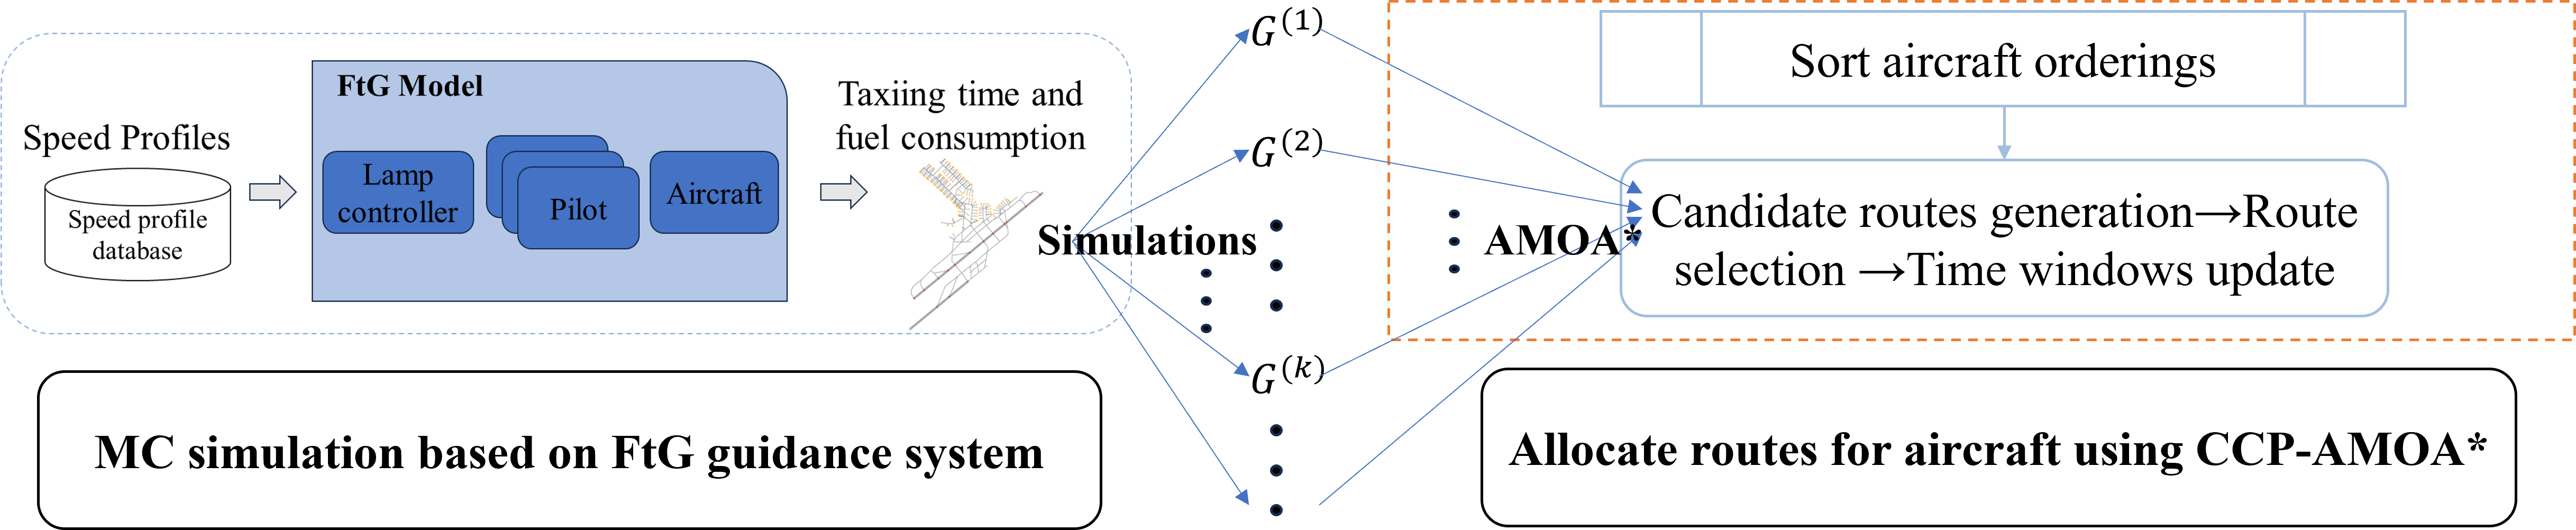
\includegraphics[width=6in]{figures/Solution approach.png}}
	\caption{Solution approach. Each MC simulation produces a distinct airport graph model $G^{(k)}$. Candidate routes are generated by searching across all graphs, thereby capturing a diverse set of potential routing options under uncertainties.}
	\label{Fig. 1}
	\vspace*{-0.5pc}
\end{figure}
%======================================================

\subsection{MC simulation based on FtG guidance system}

This section presents the MC simulation method based on the FtG guidance system for modelling taxiing time and fuel consumption with uncertainties.  \blue{The uncertainties, arising from pilot conformance errors to FtG guidance as described in~\cite{zhang2020feasibility}, are represented and propagated through MC simulations embedded in a realistic airport ground movement guidance process, enabling operationally grounded evaluation of stochastic performance. }As illustrated in Fig.~\ref{Fig. 2}, fuzzy taxiing times \cite{brownlee2018fuzzy} and a pre-established speed profile database \cite{weiszer2015real} are used to select speed profiles as simulation inputs. The FtG model serves as the foundation for uncertainties propagation, with behavioural variabilities introduced by altering parameters within the pilot model across different simulation runs. Each simulation run thus represents a unique pilot behaviour controlling the aircraft according to the selected speed profile. The resulting taxiing time and fuel consumption values are then derived from these simulated speed profiles.

%======================================================
\begin{figure}[H]
	\centerline{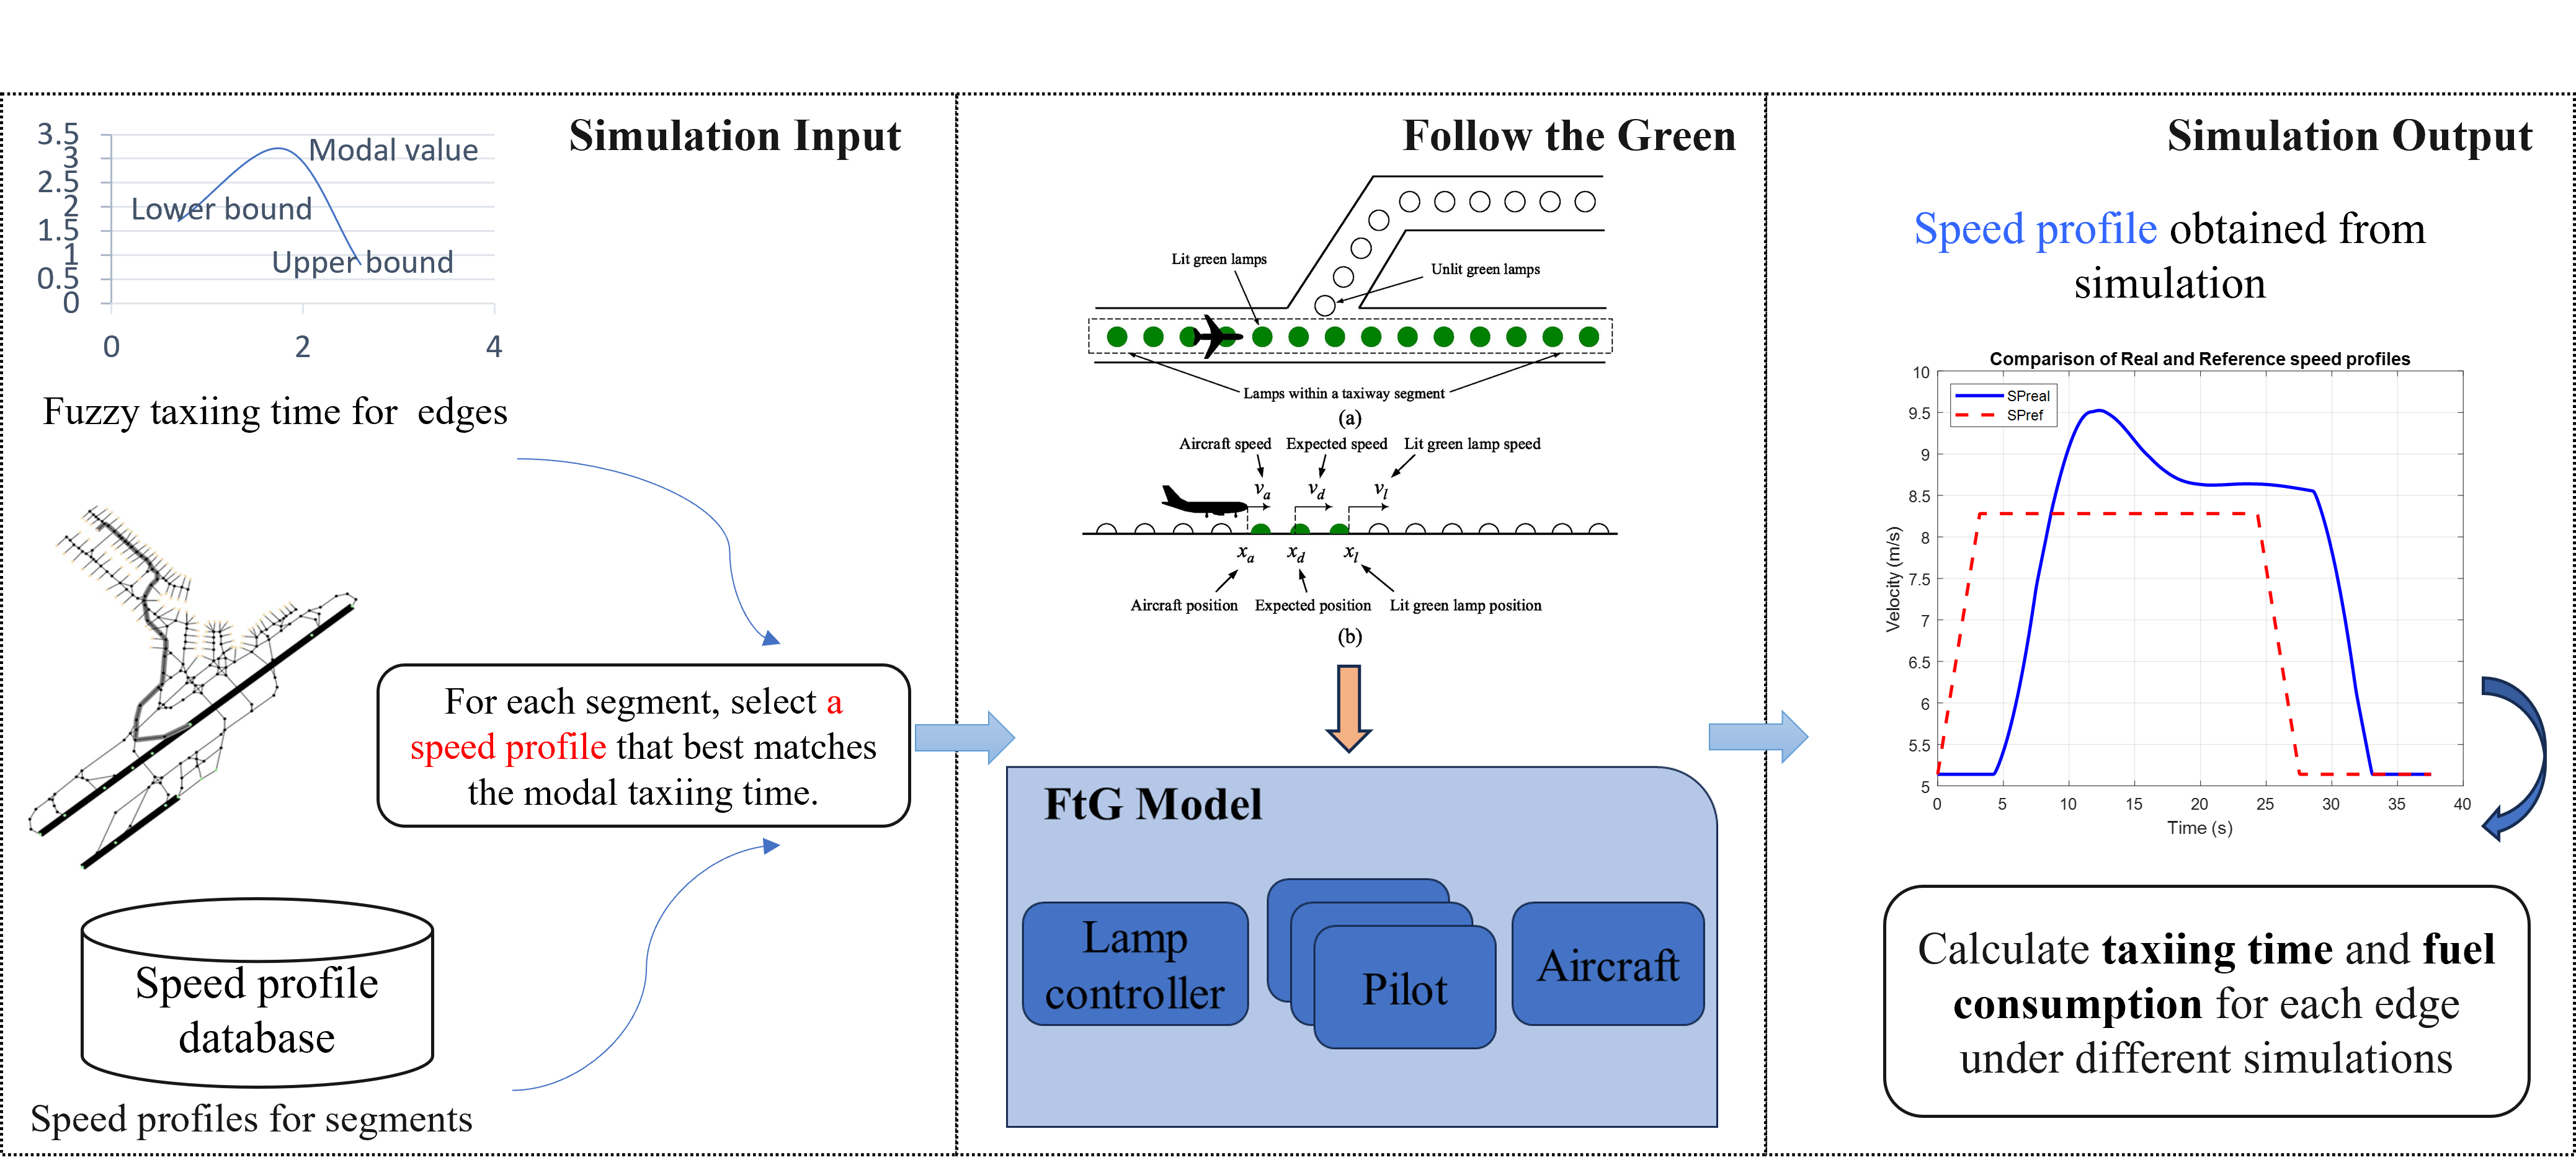
\includegraphics[width=6in]{figures/MC simulation3.png}}
	\caption{MC simulation. The reference speed profile is provided as input to the FtG model, which simulates the taxiing behaviour under the FtG guidance. The resulting speed profile is then used to calculate taxiing time and fuel consumption.}
	\label{Fig. 2}
	\vspace*{-0.5pc}
\end{figure}
%======================================================

\subsubsection{Simulation Input}

The simulation inputs are speed profiles for segments which consist of multiple edges. Weiszer et al. \cite{weiszer2015real} developed databases containing speed profiles optimised using heuristic methods, while Brownlee et al.\cite{brownlee2018fuzzy} proposed an adaptive Mamdani fuzzy rule based system to estimate taxiing times and their associated uncertainties. In their approach, the modal value of the fuzzy set is used to represent the most likely taxiing time. To ensure the simulation inputs are both optimal and realistic, the best speed profile for each segment is selected using Algorithm\ref{A1}, which aims to minimise the deviation from the most likely (modal) taxiing time. In this study, while the speed profile databases \cite{weiszer2015real} and modal taxiing times \cite{brownlee2018fuzzy} are used to select speed profiles, the selecting algorithm is independently designed. The algorithm first calculates the total modal taxiing time for the current segment by summing modal times across its edges. It then iterates over all available speed profiles in the database, selecting the one with taxiing time being the closest to the modal time, thereby ensuring both efficiency and realism in the simulation. Here we just consider one speed profile for each segment, no multi-graph \cite{weiszer2020multi} is used in the simulation input. Our focus is on the impact of pilot behaviour uncertainty within the simulation. While incorporating multiple speed profiles is feasible, it lies beyond the scope of this study.

\begin{algorithm}
    \caption{Select speed profile for each segment.}\label{A1}
    Speed profiles database for current segment $SP$, selected speed profile $SP_{best} = \emptyset$, total modal taxiing time for current segment $tt^m=0$, initial difference $D=M$\;
    \For{all edges $e$ in current segment}{
        $tt^m \gets tt^m + tt_e^m$ \;
    }
    \For{all speed profiles $SP_i$ in $SP$}{
        Get the taxiing time of $SP_i$ as $tt_i$ \;
        \If{$\text{abs}(tt_i-tt^m)<D$}{
            $SP_{best} \gets SP_i$ \;
            $D \gets \text{abs}(tt_i-tt^m)$ \;
        }
    }
    \Return $SP_{best}$
\end{algorithm}

\subsubsection{Follow the Green}

The ground-based taxi guidance system has been deployed at airports worldwide, with the FtG system serving as a prominent example \cite{zhang2020feasibility}. Consequently, we adopt the FtG system as the basis for our simulation model. The FtG provides dynamic taxi guidance by illuminating green lights along the taxiway in real time. Pilots manually adjust their speed to follow the movement pattern of the illuminated lights, which includes both their position and progression rate. Unlike fully automated taxiing systems proposed under SESAR or NextGen \cite{schuster2014performance}, FtG retains a human-in-the-loop approach, combining pilot intuition with enhanced guidance accuracy through real-time lamp sequencing. The FtG-based simulation model for aircraft taxiing consists of three main modules: the lamp controller model, the pilot driving model, and the aircraft taxiing dynamics model, as illustrated in Fig.~\ref{Fig. 3}. The lamp controller model dynamically updates the position of the illuminated lamps based on the actual aircraft position and the expected position derived from the input speed profile, using a PID controller. The pilot driving model simulates the pilot’s adjustment of engine thrust based on the distance between the aircraft and the farthest illuminated lamp. These adjustments directly affect the aircraft’s speed and position, as governed by the aircraft dynamics model. For further implementation details, readers are referred to \cite{zhang2020feasibility}.

%======================================================
\begin{figure}[htb]
	\centerline{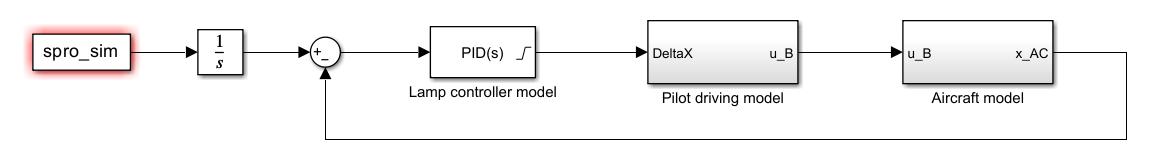
\includegraphics[width=6in]{figures/FTG-based simulation model.png}}
	\caption{FtG-based simulation model for aircraft taxiing. $spro\_sim$ represents the input speed profile; $1/s$ denotes the integrator; $Delta X$ indicates the distance between the aircraft and the farthest illuminated lamp; $u\_B$ represents the engine thrust; and $x\_AC$ denotes the actual position of the aircraft.}
	\label{Fig. 3}
	\vspace*{-0.5pc}
\end{figure}
%======================================================

In the FtG model, the parameters of the lamp controller model and the aircraft model remain fixed throughout all simulations, while those associated with the pilot driving model are stochastically sampled in each run. Specifically, the pilot driving model includes two parameters, $K_{p,1}$ and $K_{p,2}$, which characterize variations in pilot behaviour, and the pilot response time, denoted as $\tau$. The parameters $K_{p,1}$ and $K_{p,2}$ are independently drawn from uniform distributions, whereas $\tau$ is modelled as a stochastic variable following a logarithm normal distribution, capturing the natural variability in human reaction times \cite{zhang2020feasibility}. \blue{More importantly, the pilot driving model is modular: the distributional assumptions can be directly replaced by richer empirical or context-specific distributions (e.g., non-uniform or mixture models) as more comprehensive datasets become available, thereby enhancing the model’s generality without changing the overall framework.} Additionally, the aircraft model enforces maximum speed constraints that vary between turning segments and straight segments, in accordance with physical and safety limitations \cite{weiszer2020multi}.

\subsubsection{Simulation Output}

The simulation output consists of speed profiles generated by the FtG-based simulation model, representing the taxiing trajectories controlled by pilots following reference speed profiles. Then taxiing time and fuel consumption for edges in the segment can be calculated based on the simulated speed profile. The calculation of taxiing time is straightforward. While fuel consumption depends on thrust levels $\eta$ which varies according to different taxiing phases \cite{chen2016toward}. During deceleration and rapid deceleration, $\eta = 5\%$ of the full rated power. For acceleration and constant speed phases, $\eta = (\textit{weight} \cdot \textit{acc} + \mu \cdot \textit{weight} \cdot g) / F$, where $weight$ is the weight of the aircraft, $acc$ is the acceleration rate, $\mu$ is rolling resistance coefficient, $\mu \cdot \textit{weight} \cdot \textit{g}$ is the rolling resistance force, and $F$ is the maximum power output of the jet engine. The thrust level $\eta$ corresponds to a fuel flow which is calculated by linearly interpolating or extrapolating fuel flow values for $\eta = 7\%$ and $\eta = 30\%$ reported in ICAO database \cite{nikoleris2011detailed}. \blue{Note that within the MC simulation, the fuel consumption model is replaceable. For example, machine learning models can be adopted to improve accuracy across diverse operational regimes while additional empirical data becomes available.}

In addition to human factors, real-world operations are also subject to various additional sources of uncertainties, such as complex traffic interactions and dynamic environmental conditions \cite{cook2016complexity, tang2014construction}. To better reflect real operational contexts, we augment both taxiing time and fuel consumption to account for increased variability. This augmentation is guided by sampled taxiing time data under different uncertainty levels, as reported in \cite{wang2021chance}, which serve as reference benchmarks. For a given uncertainty level, the coefficient of variation is computed for each edge based on the reference data. This allows us to determine a scaling factor that adjusts the original simulation data to reflect the desired level of variability. The same scaling factor is then applied to the fuel consumption for the corresponding edge. \blue{These factors expand clusters of MC-generated taxiing time-fuel consumption pairs around their centres while preserving statistical correlations. Scaling is further constrained by aircraft performance limits (maximum speed, minimum fuel flow rate), ensuring physical feasibility. This approach maintains both edge-specific statistical relationships and fundamental physical bounds~\cite{maharana2022review}.} Through this process, we generate augmented datasets of taxiing time and fuel consumption that more accurately reflect uncertain real-world conditions.

These simulations and augmentations can be performed in advance, with each run generating a corresponding graph with different cost values. Simulations and augmentations under different uncertainty levels reflect various real-world operational conditions. Then the route allocation algorithms are developed to allocate robust, Pareto optimal taxi routes. The simulated graphs are utilised to search candidate routes for sorted aircraft, and the best route will be selected based on the MOCCP model. 

\subsection{Allocate routes for aircraft using CCP-AMOA*}

Building on the MOCCP model incorporating MC simulation, we propose the CCP-AMOA* algorithm to address the multi-objective optimisation problem for AGM under uncertainties. As illustrated in Fig.~\ref{Fig. 4}, aircraft are first sorted using a natural ordering scheme: arrival flights are prioritised by landing time, followed by departures ordered by takeoff time. Routes are then allocated sequentially using the CCP-AMOA* algorithm, as described in Section 4.2.1. This algorithm consists of three core modules: candidate route generation, route selection, and time window updating. Candidate routes are generated across multiple simulated graphs using the extended AMOA* algorithm presented in Section 4.2.2.

%======================================================
\begin{figure}[H]
	\centerline{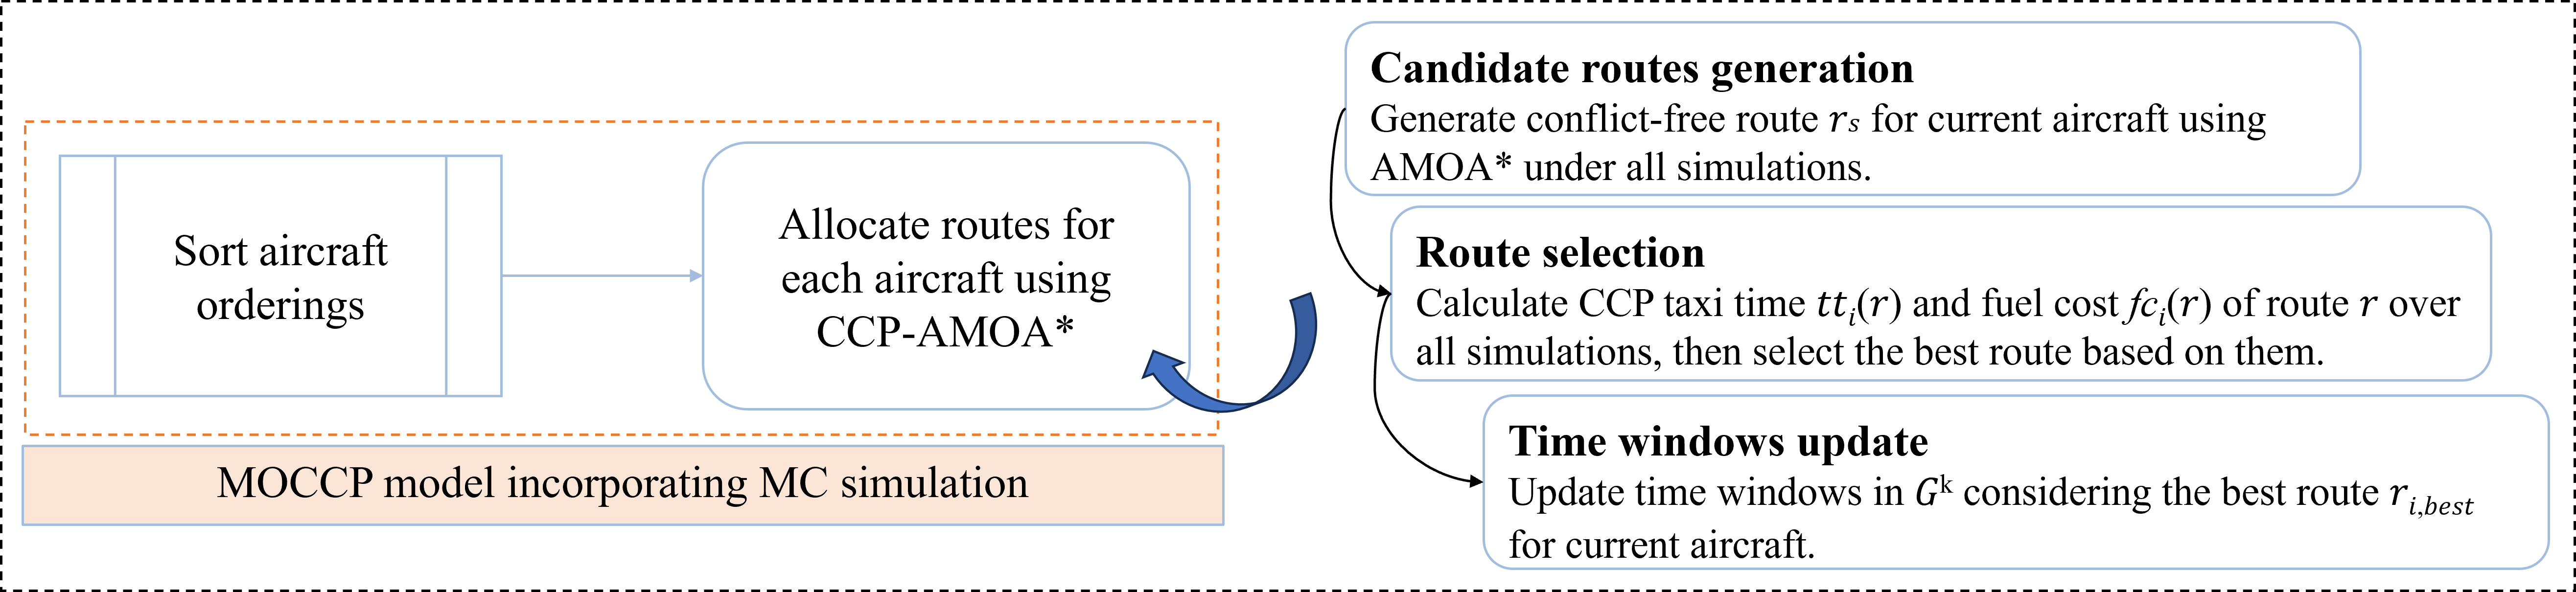
\includegraphics[width=6in]{figures/Routing algorithm.png}}
	\caption{The routing algorithm.}
	\label{Fig. 4}
	\vspace*{-0.5pc}
\end{figure}
%======================================================


\subsubsection{CCP-AMOA*}

To allocate robust Pareto-optimal routes for aircraft, we utilise the extended AMOA* algorithm (more details will be introduced in the next subsection) across multiple simulated graphs to generate non-dominated candidate routes. However, the sequential nature of aircraft routing leads to exponential growth in the search space and computational complexity. \blue{To mitigate this issue, multiple preference settings are introduced to guide the search towards different regions of the Pareto front~\cite{weiszer2020fuel}. This preference-based scalarisation strategy serves as a pragmatic compromise, substantially reducing computational complexity while providing a representative approximation of the Pareto-optimal set under the given problem constraints.} The proposed CCP-AMOA* algorithm operates as outlined in Algorithm \ref{A2}.
%======================================================================
\begin{algorithm}
	\caption{CCP-AMOA*}\label{A2}
	  Route set $R=\emptyset$, minimal taxiing time and minimal fuel consumption $tt_{i,min}=M$, $fc_{i,min}=M$, selected route $r_{i,best}=\emptyset$, preference $(\lambda_1, \lambda_2)$ \;
	\For {each graph $G^{(k)} \in \mathcal{G}$}
	{
		Generate conflict-free route $r_s$ for current aircraft using AMOA* on graph $G^{(k)}$ with simulated deterministic taxiing time and fuel consumption \;
            Add route $r_s$ in $R$ if $r_s \notin R$
        }
        \For {each route $r \in R$}
	{
		Calculate CCP taxiing time $tt_i(r)$ and fuel consumption $fc_i(r)$ over all graphs\;
        \If {$(tt_i(r),fc_i(r))(\lambda_1, \lambda_2)^{\mathrm{T}}<(tt_{i,min},fc_{i,min})(\lambda_1, \lambda_2)^{\mathrm{T}}$}
            {
                $tt_{i,min}=tt_i(r)$\;
                $fc_{i,min}=fc_i(r)$\;
                $r_{i,best}=r$
            }
        }
        \For {each graph $G^{(k)} \in \mathcal{G}$}
        {
        Update time windows for all edges in $G^{(k)}$ considering the best route $r_{i,best}$ for current aircraft
        }
        Return $r_{i,best}$
\end{algorithm}
%=======================================================================

Each graph $G^{(k)}$ with known edge costs corresponds to a deterministic multi-objective route searching problem. After generating all candidate routes across simulations using the extended AMOA* algorithm (Lines 2-4), the optimal route is selected based on the CCP values for taxiing time and fuel consumption, as well as the preferences (Lines 5-10). Based on the chance constraints in the MOCCP model, the CCP value is defined as the smallest threshold such that the constraint is satisfied in at least a specified proportion of graphs, corresponding to the confidence level, as described in \cite{wang2021chance}. For example, given five taxiing time values across five graphs for a single route: 13s, 16s, 17s, 18s and 20s, the CCP value would be 18s if the confidence level is set to 0.8, meaning the constraint must hold in at least 80\% (i.e., four out of five) of the graphs. Finally, the time windows in all graphs are updated to ensure safety and temporal feasibility, as discussed in \cite{ravizza2013trade,brownlee2018fuzzy}.

\subsubsection{AMOA*}

The AMOA* algorithm developed in \cite{weiszer2020multi} efficiently addresses the airport routing problem by considering both the accumulated costs from the origin and admissible heuristic estimates of the remaining costs to the destination. This approach systematically guides the search toward optimal solutions while avoiding inefficient exploration paths \cite{mandow2008multiobjective}.

%======================================================================
\begin{algorithm}
	\caption{AMOA*}\label{A3}
	 A search graph $SG$, two sets $G_{start}^{op}=\{(0,0)\}$, search direction indicator $backwards$, $G_{start}^{cl}={\emptyset}$ for start nodes, a list of alternatives $OPEN$, $COST={\emptyset}$ \;
         \If {!backwards}
            {
            $OPEN=\{(start, g_{start}, f_{start}, [time_{arr}, \infty)\}$ \;
            }
        \Else
            {
            $OPEN=\{(end, g_{end}, f_{start}, (0, time_{dep})\}$ \;
            }
        /* Check termination: \;
        \If {$OPEN=={\emptyset}$}
        {
            \If {!backwards}
            {
            Reconstruct routes in $SG$ from $end$ node and return set of routes $R_i$ \;
            }
            \Else
            {
            Reconstruct routes in $SG$ from $start$ node and return set of routes $R_i$ \;
            }
        }
        Select an alternative $(n,g_n,f_n,[win^a,win^b]$ from $OPEN$ \;
        Delete $(n,g_n,f_n,[win^a,win^b])$ from $OPEN$ and move $g_n$ from $G_{n}^{op}$ to $G_{n}^{cl}$ \;
	  \If {$n$ is $end$ node}
        {
        /* Solution recording: \;
        Include $g_n$ in $COSTS$ \;
        Eliminate form $OPEN$ all alternatives $(x,g_x,f_x,[win_x^a,win_x^b])$ if $g_n \prec f_n$ \;
        Go to Line 3 \;
        }
        \Else 
        {
        /* Path expansion: \;
        Expand $(n,g_n,f_n,[win^a,win^b])$ \;
        }
\end{algorithm}
%=======================================================================

\blue{Building on the algorithm in \cite{weiszer2020fuel}, the search is extended from the segment level to the edge level. Time-window attributes are also incorporated into candidate nodes during the exploration phase to enhance the search capability. In the original segment-level approach, aircraft could only stop at intersection nodes where segments meet due to conflict constraints, whereas the edge-level search enables aircraft to stop at any node once conflicts have been evaluated.} As detailed in Algorithm \ref{A3}, the process begins by initialising the search graph, including the open and closed sets for the start node, a search direction indicator (a binary variable set to $True$ for departure aircraft and $False$ for arrival aircraft), a set of candidate alternatives, and a cost-recording structure for the final routes (Lines 1–5). When termination conditions are met, optimal routes are reconstructed backwards from the end node (Lines 6-11); otherwise, the algorithm selects the most promising candidate from the alternative set (Lines 12-13). For candidates representing the end node, their incurred costs are recorded while dominated alternatives are pruned to avoid redundant exploration (Lines 14-18), while non-terminal candidates undergo path expansion (Lines 19-21) as described in Algorithm \ref{A4} \cite{weiszer2020multi}.    

%======================================================================
\begin{algorithm}
	\caption{Path expansion}\label{A4}
	  /* Path expansion: \;
        \For {All successor edges of $n$ to node $m$ without cycles in $SG$}
            {
            Read $c_{n,m}$ from the database \;
            \If {!backwards}
                {
                  \For {Each $F_e^j \in F(e)$, where $F_e^j = [a_e^j,b_e^j]$ in increasing order of $a_e^j$}
                {
                /* Expand windows for edges where time intervals overlap \;
                \If {$a_e^j>win^b$}
                    {
                    Go to Line 2 /* consider the next outgoing edge\;
                    }
                \If {$b_e^j<win^a$}
                    {
                    Go to Line 5 /* consider the next time-window \;
                    }
                Let $time_{in}=max(a_e^j,win^a)$ \;
                Let $time_{out}=time_{in}+c_{n,m,1}$ \;
                \If {$time_{out}\leq b_e^j$}
                    {
                    Let $win_m=[time_{out}, b_e^j]$
                    \textbf{break} \;
                    }
                }
                }
            \Else
                {
                \For {Each $F_e^j \in F(e)$, where $F_e^j = [a_e^j,b_e^j]$ in decreasing order of $a_e^j$}
                {
                /* Expand windows for edges where time intervals overlap \;
                \If {$b_e^j<win^a$}
                    {
                    Go to Line 2 /* consider the next outgoing edge\;
                    }
                \If {$a_e^j>win^b$}
                    {
                    Go to Line 16 /* consider the next time-window \;
                    }
                Let $time_{out}=min(b_e^j,win^b)$ \;
                Let $time_{in}=time_{out}-c_{n,m,1}$ \;
                \If {$time_{in}\geq a_e^j$}
                    {
                    Let $win_m=[a_e^j, time_{in}]$
                    \textbf{break} \;
                    }
                }
                }
            Calculate the cost of the new path found to $m$: $g_m=g_n+c_{n,m}$ \;
            \If {$m$ is not in $SG$}
                {
                Calculate $f_m=g_m+H(m,end)$ \;
                \If {$f_m$ is not dominated by any vectors in $COSTS$}
                    {
                    Put $(m,g_m,f_m,win_m)$ in $Open$ \;
                    Put $g_m$ in $G_{m}^{op}$ \;
                    Create edge $(m,n)$ in $SG$ with labels $g_m$ and $c_{n,m}$ \;
                    }
                }
            \ElseIf {$g_m$ equals some cost vector in $G_{m}^{op} \cup G_{m}^{cl}$}
                {
                Create edge $(m,n)$ in $SG$ with labels $g_m$ and $c_{n,m}$ \;
                }
            \ElseIf {$g_m$ is not dominated by any cost vector in $G_{m}^{op} \cup G_{m}^{cl}$} 
                {
                /* a path to $m$ with new interesting cost has been found \;
                Eliminate $G_{m}^{op} \cup G_{m}^{cl}$ from vectors dominated by $g_m$. For each vector $g_m^{'}$ eliminated from $G_{m}^{op}$, eliminate the corresponding $(m,g_m^{'},f_m,[win^{a'},win^{b'}])$ from $OPEN$ \;
                 Calculate $f_m=g_m+H(m,end)$ \;
                \If {$f_m$ is not dominated by any vectors in $COSTS$}
                    {
                    Put $(m,g_m,f_m,win_m)$ in $Open$ \;
                    Put $g_m$ in $G_{m}^{op}$ \;
                    Create edge $(m,n)$ in $SG$ with labels $g_m$ and $c_{n,m}$ \;
                    }
                }
            }
\end{algorithm}
%=======================================================================

Due to the differing search directions for arrival and departure aircraft, the path expansion process varies in how time windows are compared. For arrival aircraft, expansion proceeds forward: once an overlapping time interval is detected, the taxi-in time is determined first, followed by the taxi-out time (Lines 4–14). For departure aircraft, expansion occurs in reverse, so the taxi-out time is established first, then the taxi-in time (Lines 15–25). Once a feasible successor edge is identified, the incurred cost is updated by adding the cost of traversing that edge (Line 26). The search graph is expanded under three conditions: if the explored node is not yet present in the graph (Lines 27–32); if it already exists and the new incurred cost matches an existing cost in the open or closed sets (Lines 33–34); or if it exists but the new cost is not dominated by any existing costs (Lines 35–42). A heuristic function 
$H$ is used to guide the search and reduce redundancy by estimating a lower bound on the remaining cost from the current node to the goal (Line 28 and Line 38). Specifically, the heuristic for taxiing time is calculated as the shortest remaining distance divided by the maximum allowable speed, while the heuristic for fuel consumption is estimated by multiplying the taxiing time by the fuel flow rate at a constant speed.

\section{Experimental results and discussions}

\subsection{Experimental setup}

Manchester Airport (MAN), the third busiest airport in the United Kingdom, is selected to evaluate the performance of our proposed model and algorithm. The graph model is constructed by preprocessing the layout of MAN as developed in \cite{brownlee2018fuzzy}, shown in Fig.~\ref{Fig. 5}. Additionally, a set of realistic aircraft movement data for one day of operations was provided by MAN. To create varying traffic scenarios, we replicated and modified the original data by introducing a two-minute offset to the scheduled departure or arrival times. This resulted in multiple datasets representing different traffic densities: low (0.8× the original movements), moderately low (0.9×), realistic (baseline, 1.0×), moderately high (1.1×), and high (1.2× the original movements). The exact number of aircraft movements for each density level is detailed in Table \ref{movements numbers}.

%======================================================
\begin{figure}[H]
	\centerline{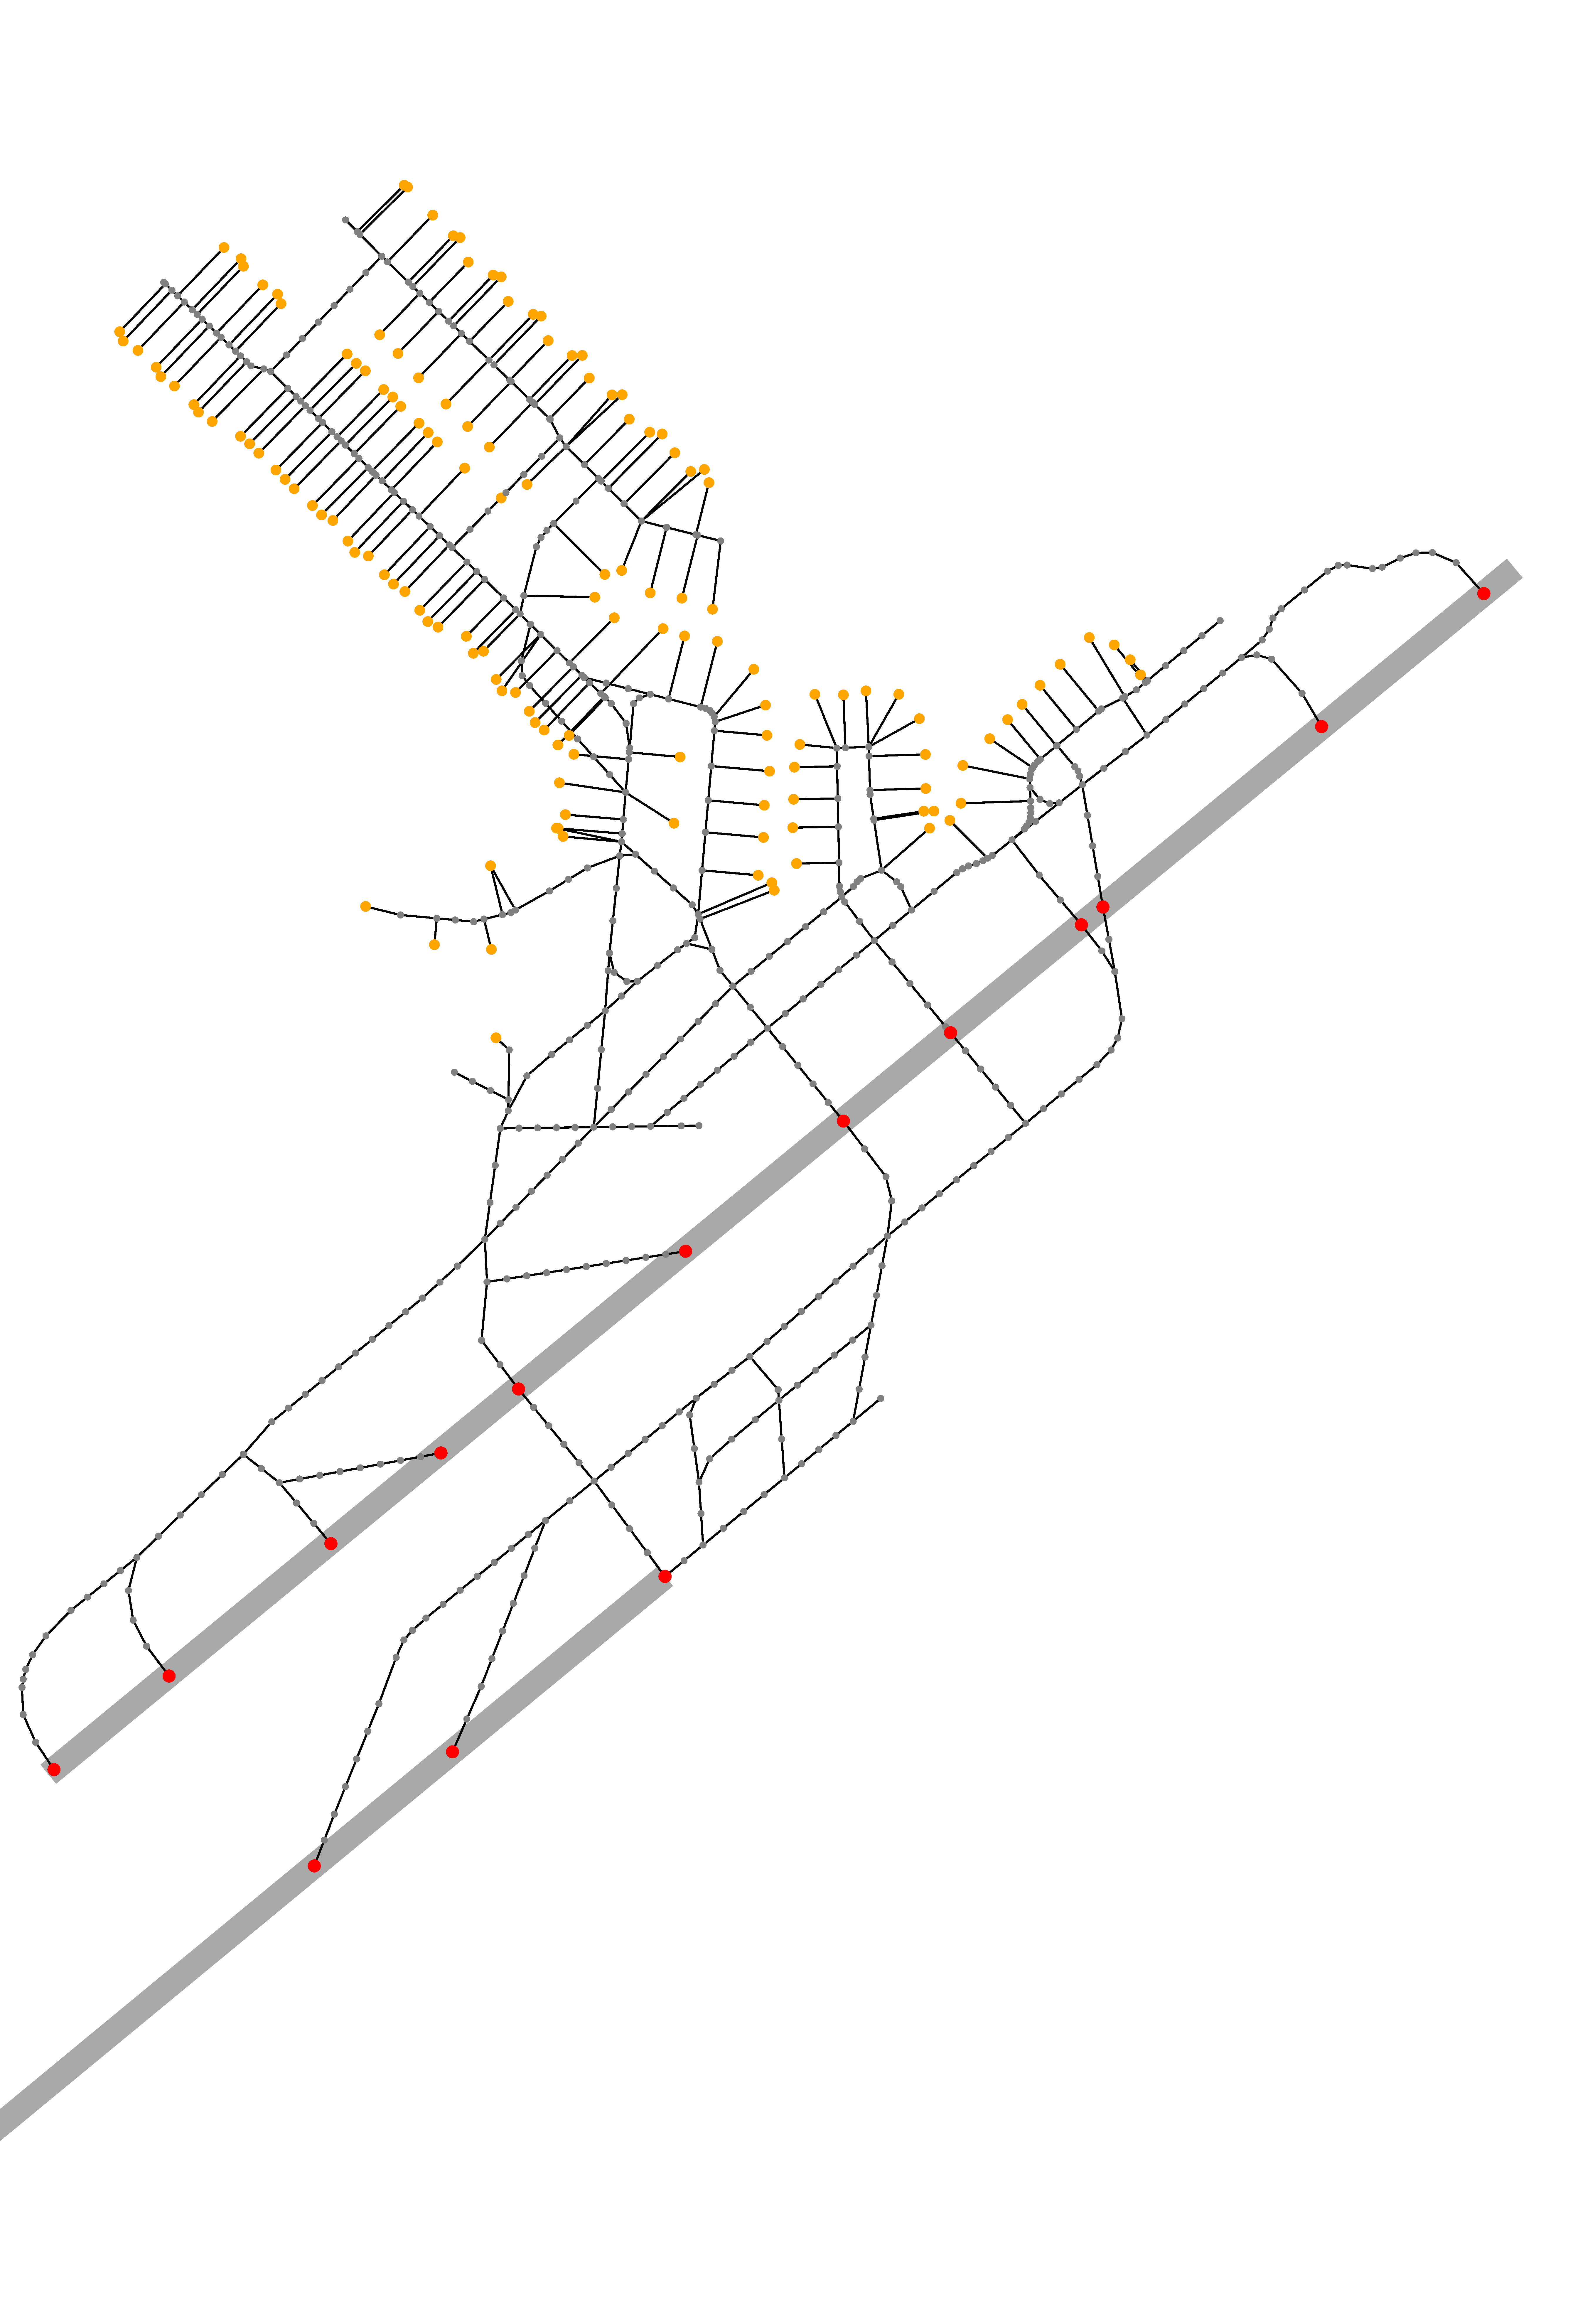
\includegraphics[width=3.5in, trim=0cm 20cm 0cm 10cm, clip]{figures/man_network3.pdf}}
	\caption{The undirected graph representing MAN ground movement network consists of 671 nodes and 714 edges, including 147 gates (orange) and 15 runway exits (red). Notably, two active runways are excluded from the network, as taxiing is prohibited on runways during normal operations.}
	\label{Fig. 5}
	\vspace*{-0.5pc}
\end{figure}
%======================================================

\begin{table}[ht]
    \centering
    \caption{Aircraft movement counts across traffic densities.}
    \begin{tabular}{llllll}
        \toprule
         Density & 0.8 & 0.9 & 1.0 & 1.1 & 1.2\\
        \midrule
        Number of aircraft movements & 516 & 575 & 640 & 701 & 790 \\
        \bottomrule
    \end{tabular}
    \label{movements numbers}
\end{table}

For the MC simulation, we select the Airbus A320 as the representative aircraft model due to its predominance in MAN operations, with its key performance parameters $\gamma$ detailed in Table \ref{a320 parameters}. For the lamp controller, the parameters $\alpha$ primarily include the PID control values: proportional gain $P = 2$, integral gain $I = 0.1$, and derivative gain $D = 3$. For the pilot model, the response time $\tau$ follows the logarithm normal distribution, and its probability density function is described as $p(\tau) = \frac{1}{\tau \sigma \sqrt{2\pi}} \exp\left( -\frac{(\ln \tau - \mu)^2}{2\sigma^2} \right)$, where $\mu=1.67$ according to the mean pilot response time $\bar{\tau}=5.29$ and $\sigma=0.2$  \cite{zhang2020feasibility}. As the parameters account for the characteristics of pilot driving behaviours, $K_{p,1} \sim \text{Uniform}(0.0001613,\ 0.0002113)$ and $K_{p,2} \sim \text{Uniform}(0.0312,\ 0.0362)$ \cite{zhang2020feasibility}.

\begin{table}[ht]
    \centering
    \caption{Airbus A320 parameters.}
    \begin{tabular}{ll}
        \toprule
        \textbf{Parameter} & \textbf{Value} \\
        \midrule
        Aircraft mass & 78000 $kg$ \\
        Rolling resistance coefficient & 0.015 \\
        Rated thrust & 222.4 $kN$ \\
        Fuel flow rate at 7\% rated thrust & 0.101 $kg/s$ \\
        Fuel flow rate at 30\% rated thrust & 0.291 $kg/s$ \\
        \bottomrule
    \end{tabular}
    \label{a320 parameters}
\end{table}

To evaluate the performance of routes allocated by the algorithm at MAN, we utilise the Java-based simulation platform developed by \cite{brownlee2018fuzzy}, which provides a high-fidelity replication of airport operations through three critical mechanisms: enforcement of minimum separation distances and mandatory stopping protocols to ensure conflict-free operations and constraint satisfaction; high-resolution aircraft position updates at 0.1-second intervals; and stringent runway occupancy management, incorporating 2-minute pre-arrival and 1-minute post-departure taxiway blocking periods to maintain operational safety margins. It should be noted that the MC simulation and the Java-based simulation serve different purposes. The MC simulation propagates uncertainties to generate graphs with different cost values, while the Java-based simulation uses these costs to evaluate the performance of allocated routes.

\subsection{Results and discussions}

\subsubsection{Taxiing time and fuel consumption with uncertainties}

After conducting the MC simulations, we analyse the distributions of taxiing time and fuel consumption across multiple runs for various taxiway edges. 

\begin{figure}[htp]
    \centering
    \subfloat[Edges in straight segments for arrival aircraft\label{fig:arr_straight}]{
        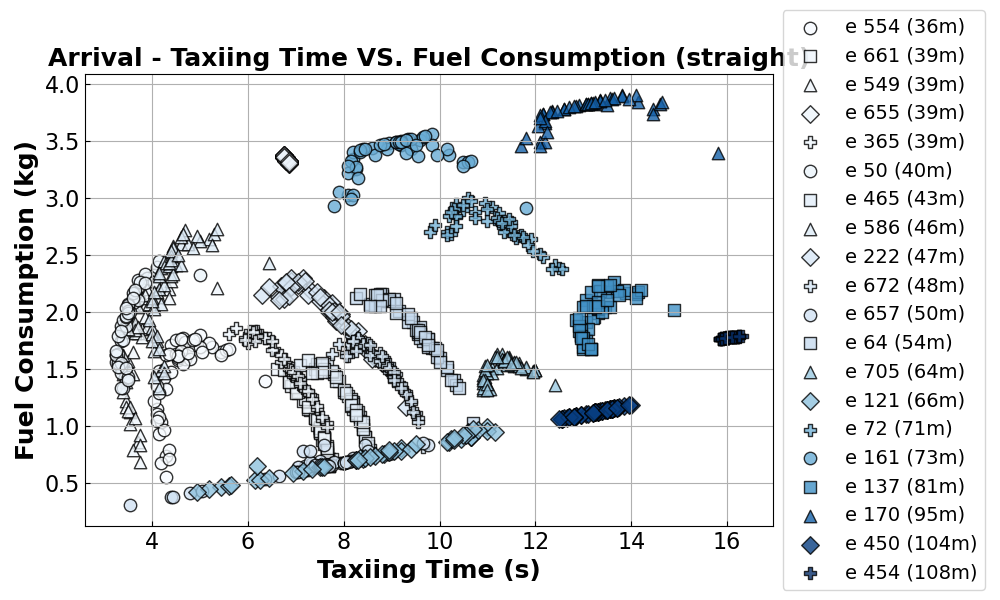
\includegraphics[width=0.46\textwidth]{figures/MC simulation results/arr_s.png}
    }
    \hfill
    \subfloat[Edges in turning segments for arrival aircraft\label{fig:arr_turning}]{
        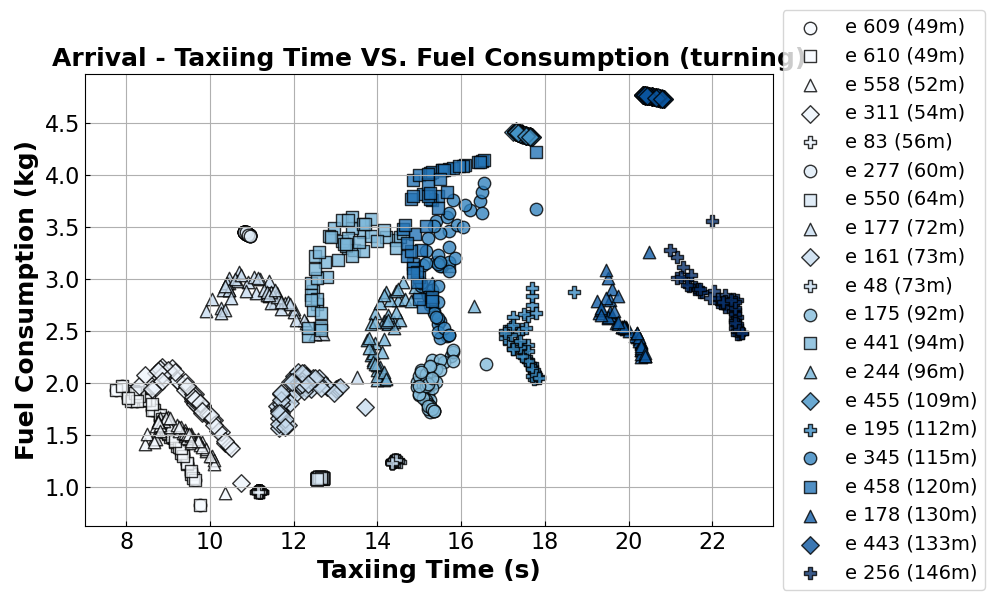
\includegraphics[width=0.46\textwidth]{figures/MC simulation results/arr_t.png}
    }
    
    \subfloat[Edges in straight segments for departure aircraft\label{fig:dep_straight}]{
        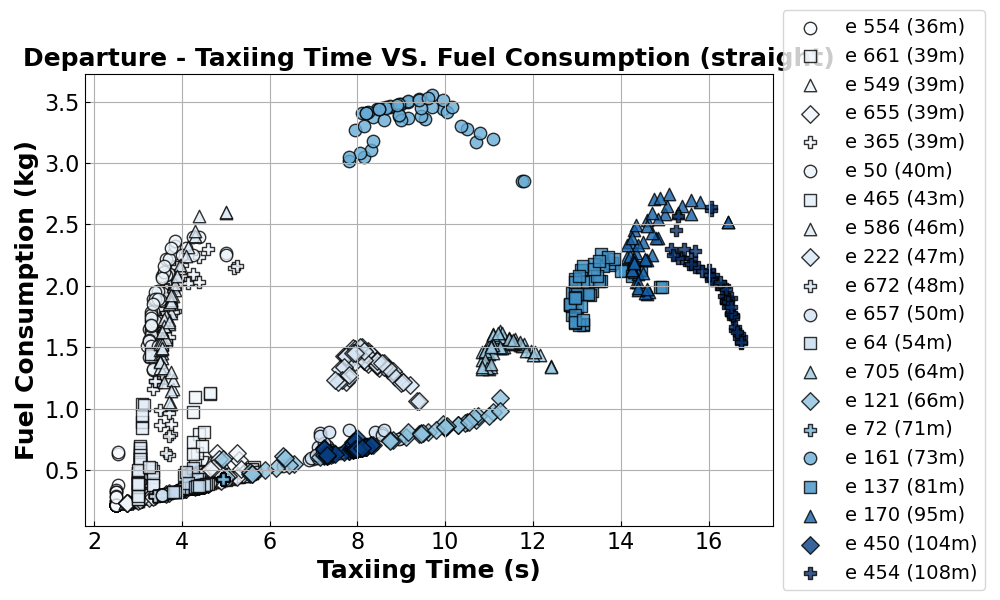
\includegraphics[width=0.46\textwidth]{figures/MC simulation results/dep_s.png}
    }
    \hfill
    \subfloat[Edges in turning segments for departure aircraft\label{fig:dep_turning}]{
        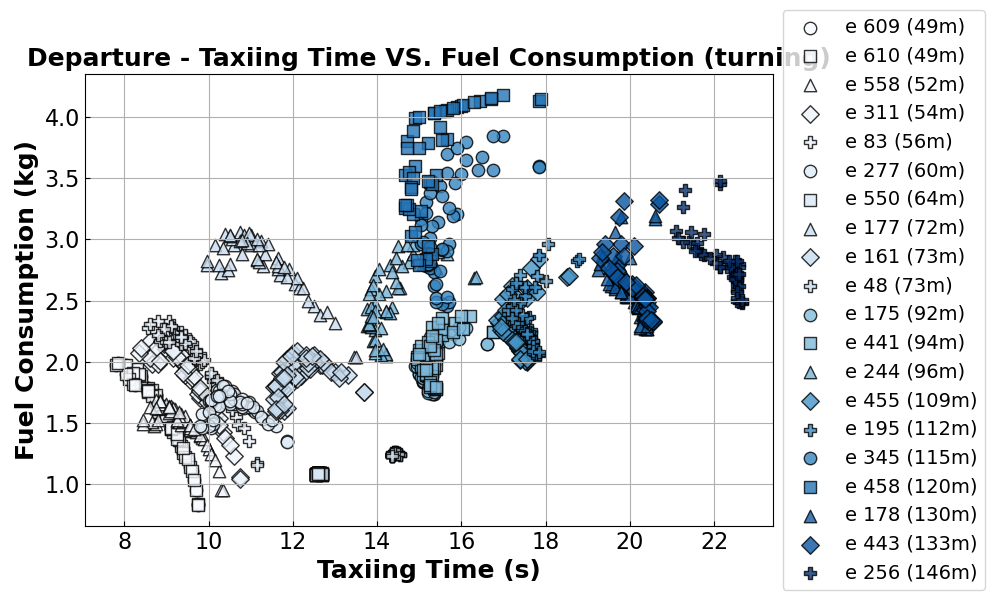
\includegraphics[width=0.46\textwidth]{figures/MC simulation results/dep_t.png}
    }
    
    \caption{MC simulation results for taxiing time and fuel consumption across edges. }
    \label{fig:MC}
\end{figure}

As illustrated in Fig.~\ref{fig:MC}, longer taxiing distances generally correspond to increased taxiing times and higher fuel consumption, indicating an overall  positive correlation. However, this trend is not consistent across all edges. For example, $e$177 is shorter than $e$161, yet it exhibits higher fuel consumption on average as illustrated in Figs.~\ref{fig:arr_turning} and \ref{fig:dep_turning}. A closer examination of the clustered distributions reveals that different edges exhibit distinct relational patterns between taxiing time and fuel consumption across simulations. For instance, $e$121 shows a strong and consistent positive correlation as illustrated in Figs.~\ref{fig:arr_straight} and \ref{fig:dep_straight}, whereas $e$610 demonstrates a negative relationship as illustrated in Figs.~\ref{fig:arr_turning} and \ref{fig:dep_turning}. Interestingly, edges such as $e$705 and $e$161 exhibit hybrid behaviours, with both positive and inverse associations appearing in different regions of their distributions as illustrated in Figs.~\ref{fig:arr_straight} and \ref{fig:dep_straight}. Additionally, for straight segments, the distribution for the same edge can vary significantly depending on the direction of aircraft movement. This variability arises because an edge may correspond to different taxiing phases depending on the taxiing direction. In contrast, edges located within turning segments tend to exhibit more consistent distributions as illustrated in Figs.~\ref{fig:arr_turning} and \ref{fig:dep_turning}, as aircraft are typically controlled to maintain a constant speed while navigating turns \cite{weiszer2020multi}.

These heterogeneous distributions indicate that the impact of uncertainties on cost values varies considerably across the airport network, complicating the trade-off analysis required for cost-efficient route allocation under uncertain conditions. Furthermore, real-world operations are affected by other sources of uncertainties, such as the inaccuracy of surveillance systems, traffic interactions and dynamic environmental factors \cite{cook2016complexity, tang2014construction}. To account for varying levels of uncertainties, we augment the simulation data by aligning the coefficients of variation (CV) with those derived from realistic, fuzzy-sampling-based taxiing time in \cite{wang2021chance}. Here, the CV is a statistical measure of relative variability, which expresses the standard deviation of a dataset as a percentage of its mean \cite{abdi2010coefficient}. Corresponding simulation datasets are generated under different uncertainty levels, denoted as $un$, where $un\in \{0.1,0.2,0.3,0.4\}$ \cite{wang2021chance}. For each level, the CVs of the original simulation data are adjusted to match those of the reference data. As the uncertainty level increases, the CVs become larger overall, reflecting greater variability in the simulations. Fig.~\ref{Fig: CV} compares the CV distribution of the augmented data against the reference data at an uncertainty level of 0.3. The augmented data across four uncertainty levels are combined with five distinct traffic densities to represent a wide range of real-world operational conditions for algorithm testing. Specifically, the augmented data consist of multiple simulated graphs used for route searching, while the aircraft movement data under varying traffic densities provide diverse input.

%======================================================
\begin{figure}[htp]
	\centerline{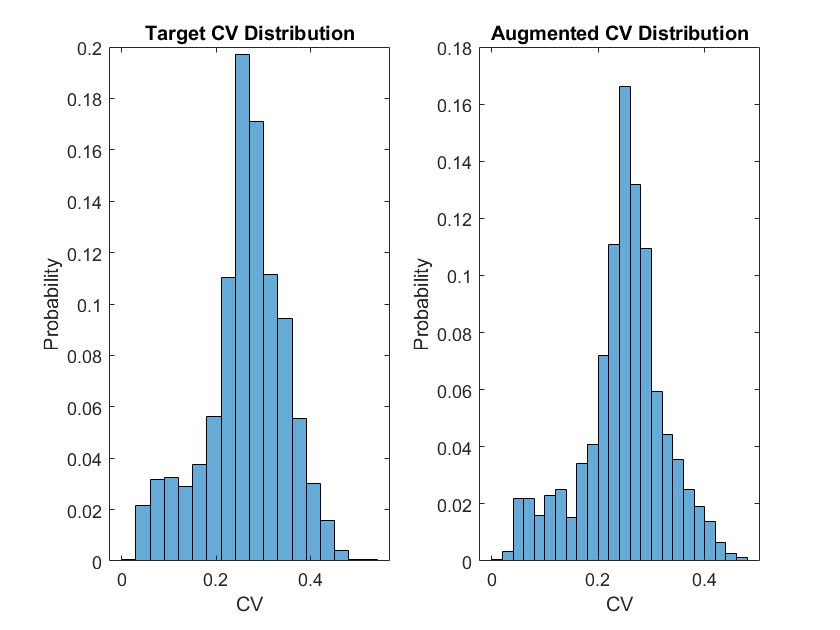
\includegraphics[width=4in]{figures/MC simulation results/cv comparison.png}}
	\caption{The CV distributions of the reference data and the augmented data under uncertainty level 0.3. The resulting Kullback–Leibler (KL) divergence \cite{kullback1951information} is 0.058, indicating a high degree of similarity between the two distributions.}
	\label{Fig: CV}
	\vspace*{-0.5pc}
\end{figure}
%======================================================
 
\subsubsection{Routed results}

The CCP-AMOA* algorithms developed in this study are denoted as \texttt{moccp}$\_\alpha\_\beta$ where $(\alpha, \beta) \in \{(0.5,0.5),\\ (0.5,1),(0.8,0.8),(0.8,1),(1,0.5)(1,0.8),(1,1)\}$, representing the confidence levels associated with taxiing time and fuel consumption, respectively. As illustrated in Algorithm \ref{A2}, these confidence levels directly influence the route selection process, allowing the solution conservativeness to be tuned in accordance with different operational priorities. Additionally, the preferences are set as $(0,1), (0.1,0.9), \ldots, (1,0)$, representing a gradual shift in priority from minimising fuel consumption to minimising taxiing time. For each aircraft, candidate routes are generated using Algorithm \ref{A3} across 30 MC simulations. The choice of 30 simulation runs follows the recommendation in \cite{wang2021chance}, providing a balance between computational efficiency and adequate representation of uncertainties.

To evaluate the effectiveness of the proposed CCP-AMOA* algorithm, the deterministic AMOA* algorithm is adopted as a baseline. The nominal values for both objectives in AMOA* are defined using one of two strategies, based on the observations from all MC simulations: (i) the average values, and (ii) the worst-case (maximum) values. These baseline variants are denoted as \texttt{amoa} and \texttt{amoa2}, respectively.

For each combination of traffic density and uncertainty level, the routes allocated by each algorithm are evaluated through 30 independent runs on Java-based simulation platform. This results in a total of 
9×11×4×5×30=59,400 simulation runs, covering 9 algorithms (2 variants of the baseline and 7 CCP-AMOA* algorithms with different confidence levels), 11 preference settings, 4 uncertainty levels, 5 traffic density levels, and 30 random repetitions. All simulations are executed on Queen Mary University of London's Apocrita high-performance computing cluster Apocrita (\url{http://doi.org/10.5281/zenodo.438045}). It should be noted that the simulations reported next in this section were performed using the Java-based simulation platform, as opposed to MC simulations. 

\vspace{0.5em}
\textbf{Pareto Front comparison.}
\vspace{0.5em}

\blue{We first present the Pareto front results to compare the overall performance of the two baseline variants and proposed algorithms. For visualisation, we extract a single representative Pareto front from the combined solutions of all algorithms per simulation, showing results from five representative simulations. Additionally, pie charts provide statistical summaries of the final robust efficient points across all 30 simulations.}

Following \cite{ide2016robustness}, a solution is considered flimsily robust efficient if it is Pareto-efficient in at least one simulation. An algorithm is judged to perform better if it discovers more such points than competing methods. Note that a single flimsily robust efficient solution may correspond to multiple points across different simulations. If a solution appears in all 30 simulations, it is regarded as highly robust efficient \cite{ide2016robustness}. In our experiments, however, highly robust efficient solutions were almost non-existent. Therefore, we count the total number of flimsily robust efficient points as our robustness indicator, rather than focusing only on highly robust efficient solutions.

Figs.~\ref{fig:td1}–\ref{fig:td2} present the results under an uncertainty level of 0.3 across traffic densities ranging from 0.8 to 1.2, while Fig.~\ref{fig:un} shows the performance at a fixed traffic density of 1.0 under varying uncertainty levels from 0.1 to 0.4. Several key observations can be drawn:

\setlength{\itemsep}{0pt}
\begin{itemize}
    \item \textbf{Observations under fixed uncertainties (0.3):} The algorithms \texttt{moccp\_0.8\_0.8}, \texttt{moccp\_1\_0.5}, and \texttt{moccp\_1\_0.8} generally outperform others across different traffic densities. These algorithms tend to favour solutions that are conservative in taxiing time while maintaining moderate fuel efficiency. Some algorithms, such as \texttt{moccp\_1\_0.5}, identify an increasing number flimsily robust efficient points (more Pareto-efficient solutions across all simulations) as traffic density rises, whereas others, like \texttt{moccp\_0.8\_0.8}, exhibit the opposite trend.
    
    \item \textbf{Observations under fixed traffic density (1.0):} The algorithm \texttt{moccp\_1\_0.5} consistently ranks among the top two performers across all uncertainty levels, suggesting that prioritising conservatism in taxiing time (with less conservatism in fuel consumption) leads to more robust solutions. In contrast, the performance of other algorithms fluctuates significantly. For example, \texttt{moccp\_1\_0.8} performs well under lower uncertainties but deteriorates as uncertainties increase.
    
    \item \textbf{Effect of asymmetric confidence levels:} Algorithms with higher confidence levels in taxiing time than in fuel consumption (e.g., \texttt{moccp\_1\_0.8}, \texttt{moccp\_1\_0.5}) tend to yield solutions with higher taxiing times but lower fuel consumption. In contrast, configurations with higher confidence in fuel consumption (e.g., \texttt{moccp\_0.8\_1}, \texttt{moccp\_0.5\_1}) favour lower taxiing times at the expense of increased fuel consumption. When the confidence levels are equal (e.g., \texttt{moccp\_0.5\_0.5}), the objectives compete more directly, resulting in a broader and more diverse Pareto front. However, this also leads to fewer flimsily robust efficient points, indicating that such diverse solutions appear less frequently across simulations.
    
    \item \textbf{Baseline variants:} They contribute relatively few solutions, typically clustered in the upper-left region of the Pareto front, indicating lower taxiing times but substantially higher fuel consumption.
\end{itemize}

Overall, the proposed algorithms exhibit superior robustness and solution quality across a wide range of traffic and uncertainty conditions, significantly outperforming the baselines.

\begin{figure}[htp]
    \centering
    
    \subfloat[Traffic density = 0.8\label{fig:td1_a}]{
        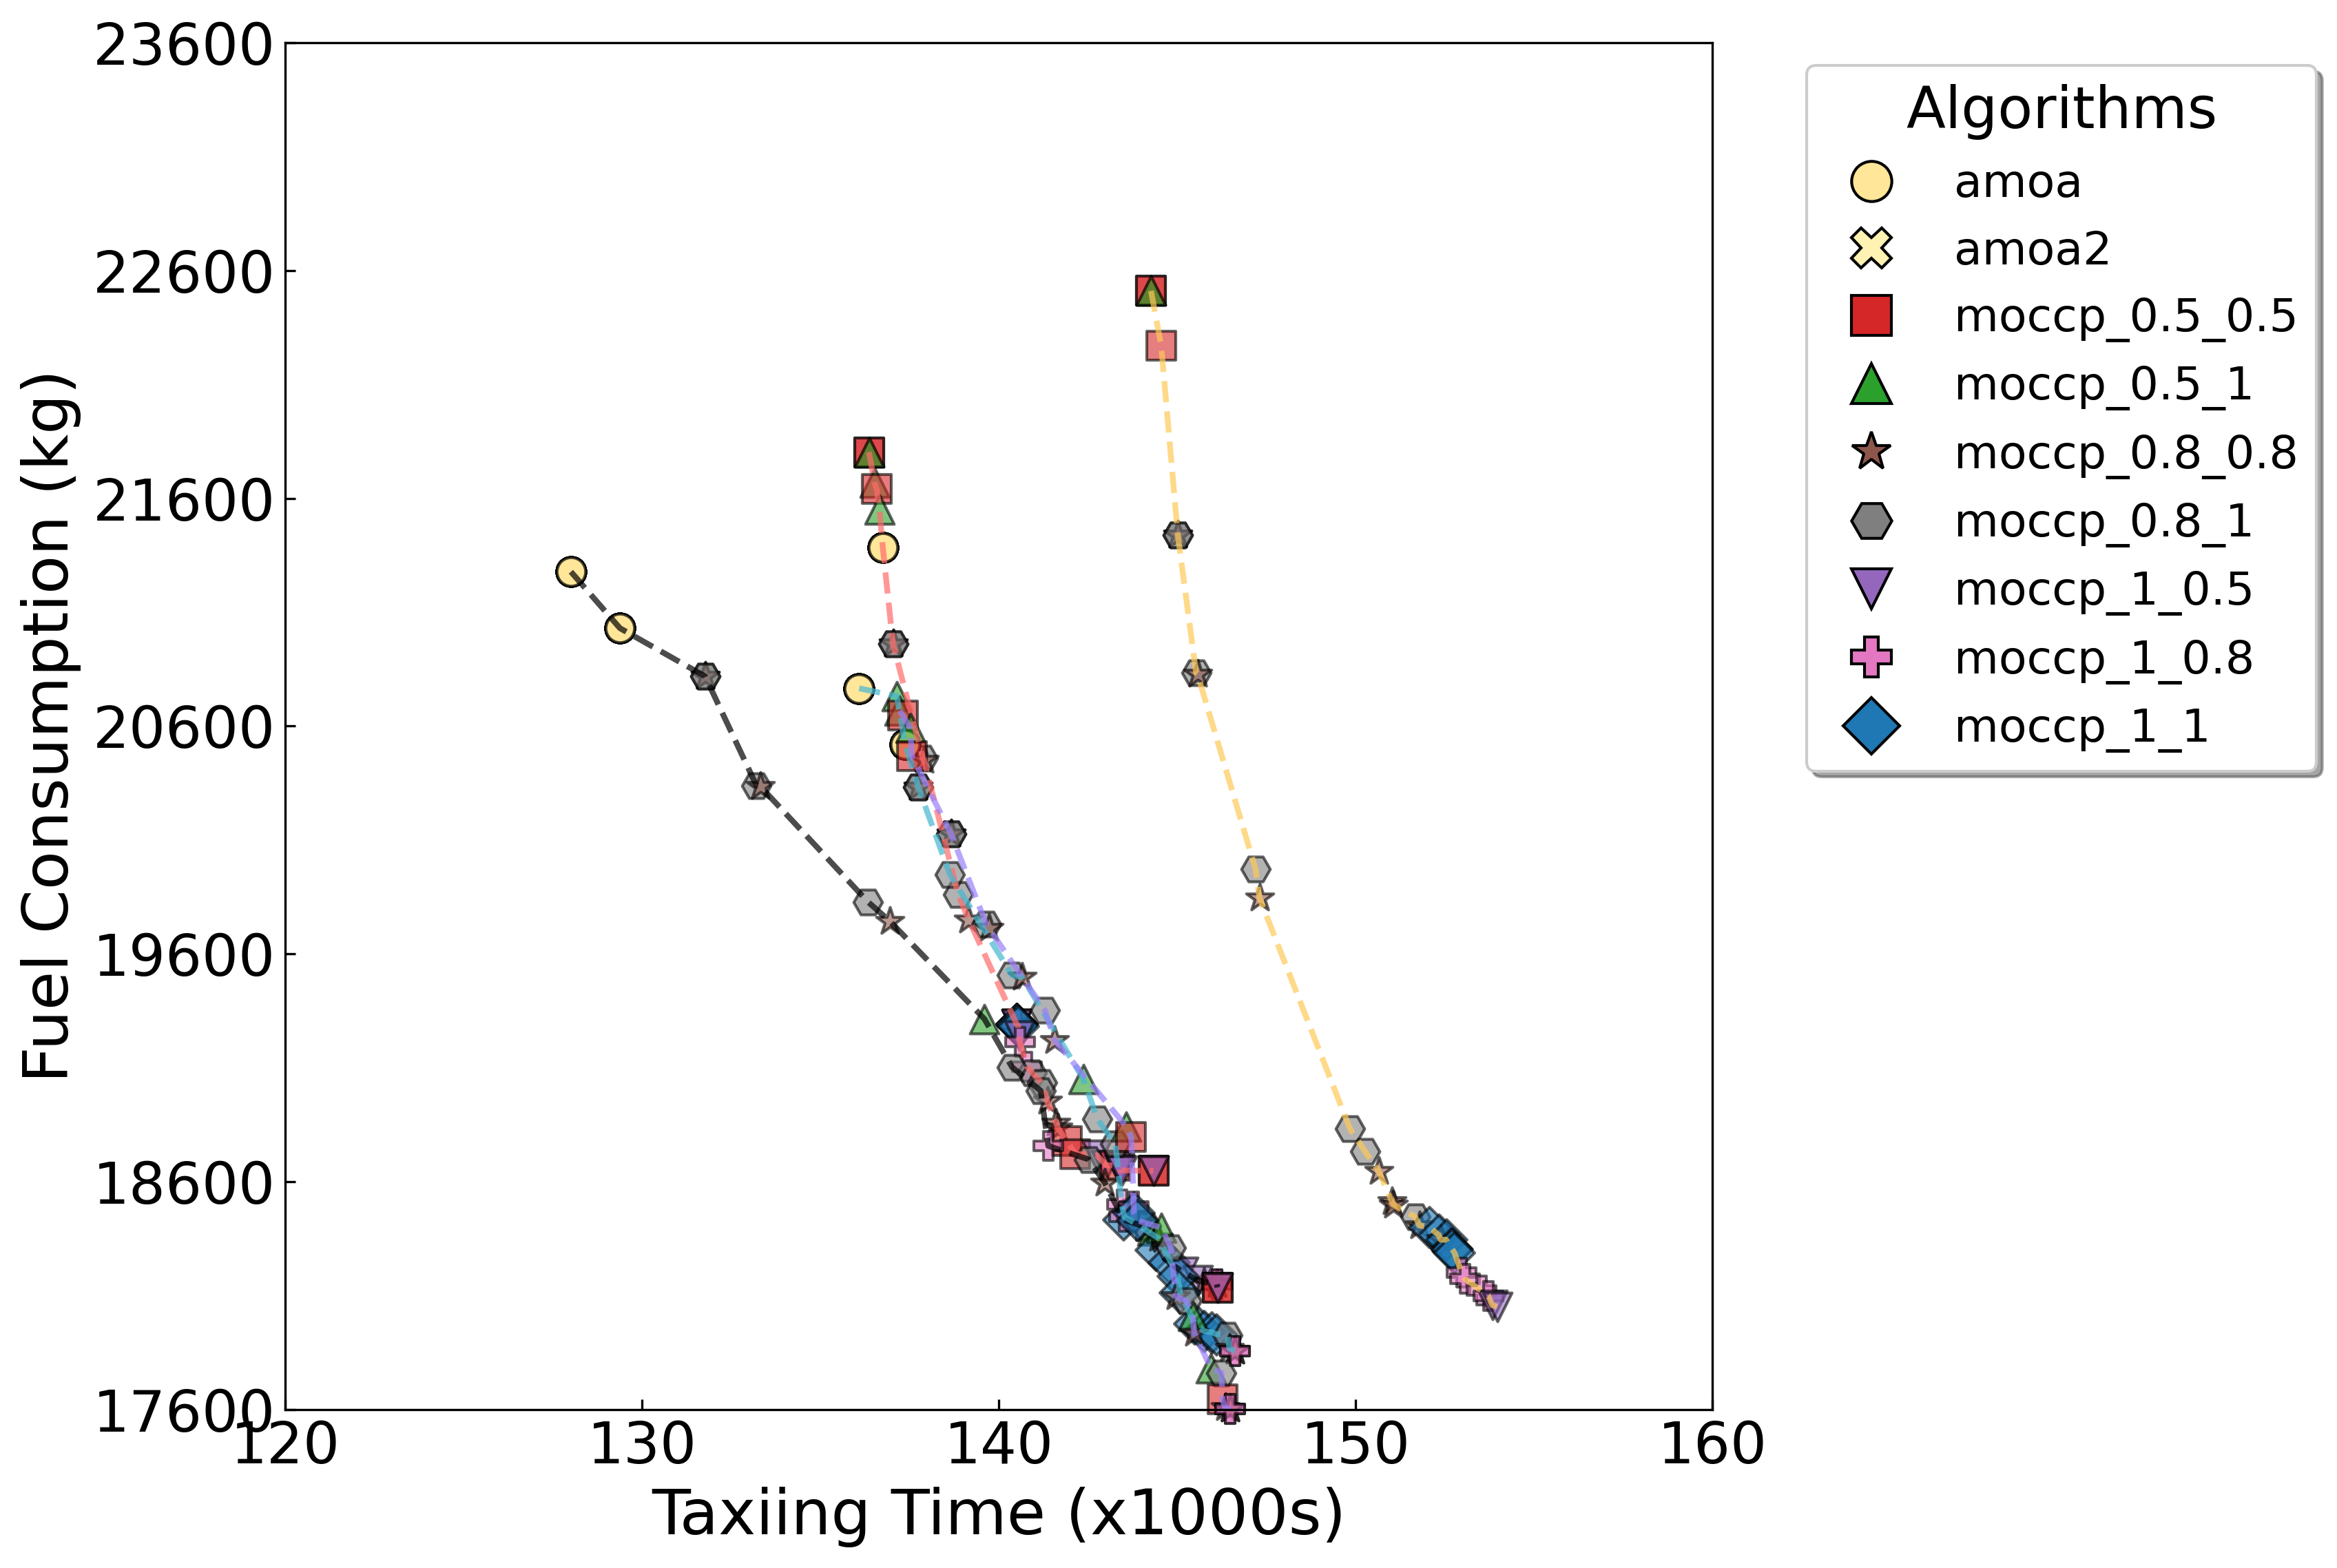
\includegraphics[width=0.45\textwidth]{figures/Un_0.3(PF)/0.8/pareto_fronts_colored.png}
    }
    \hspace{0.02\textwidth} 
    \subfloat[Traffic density = 0.8\label{fig:td1_b}]{
        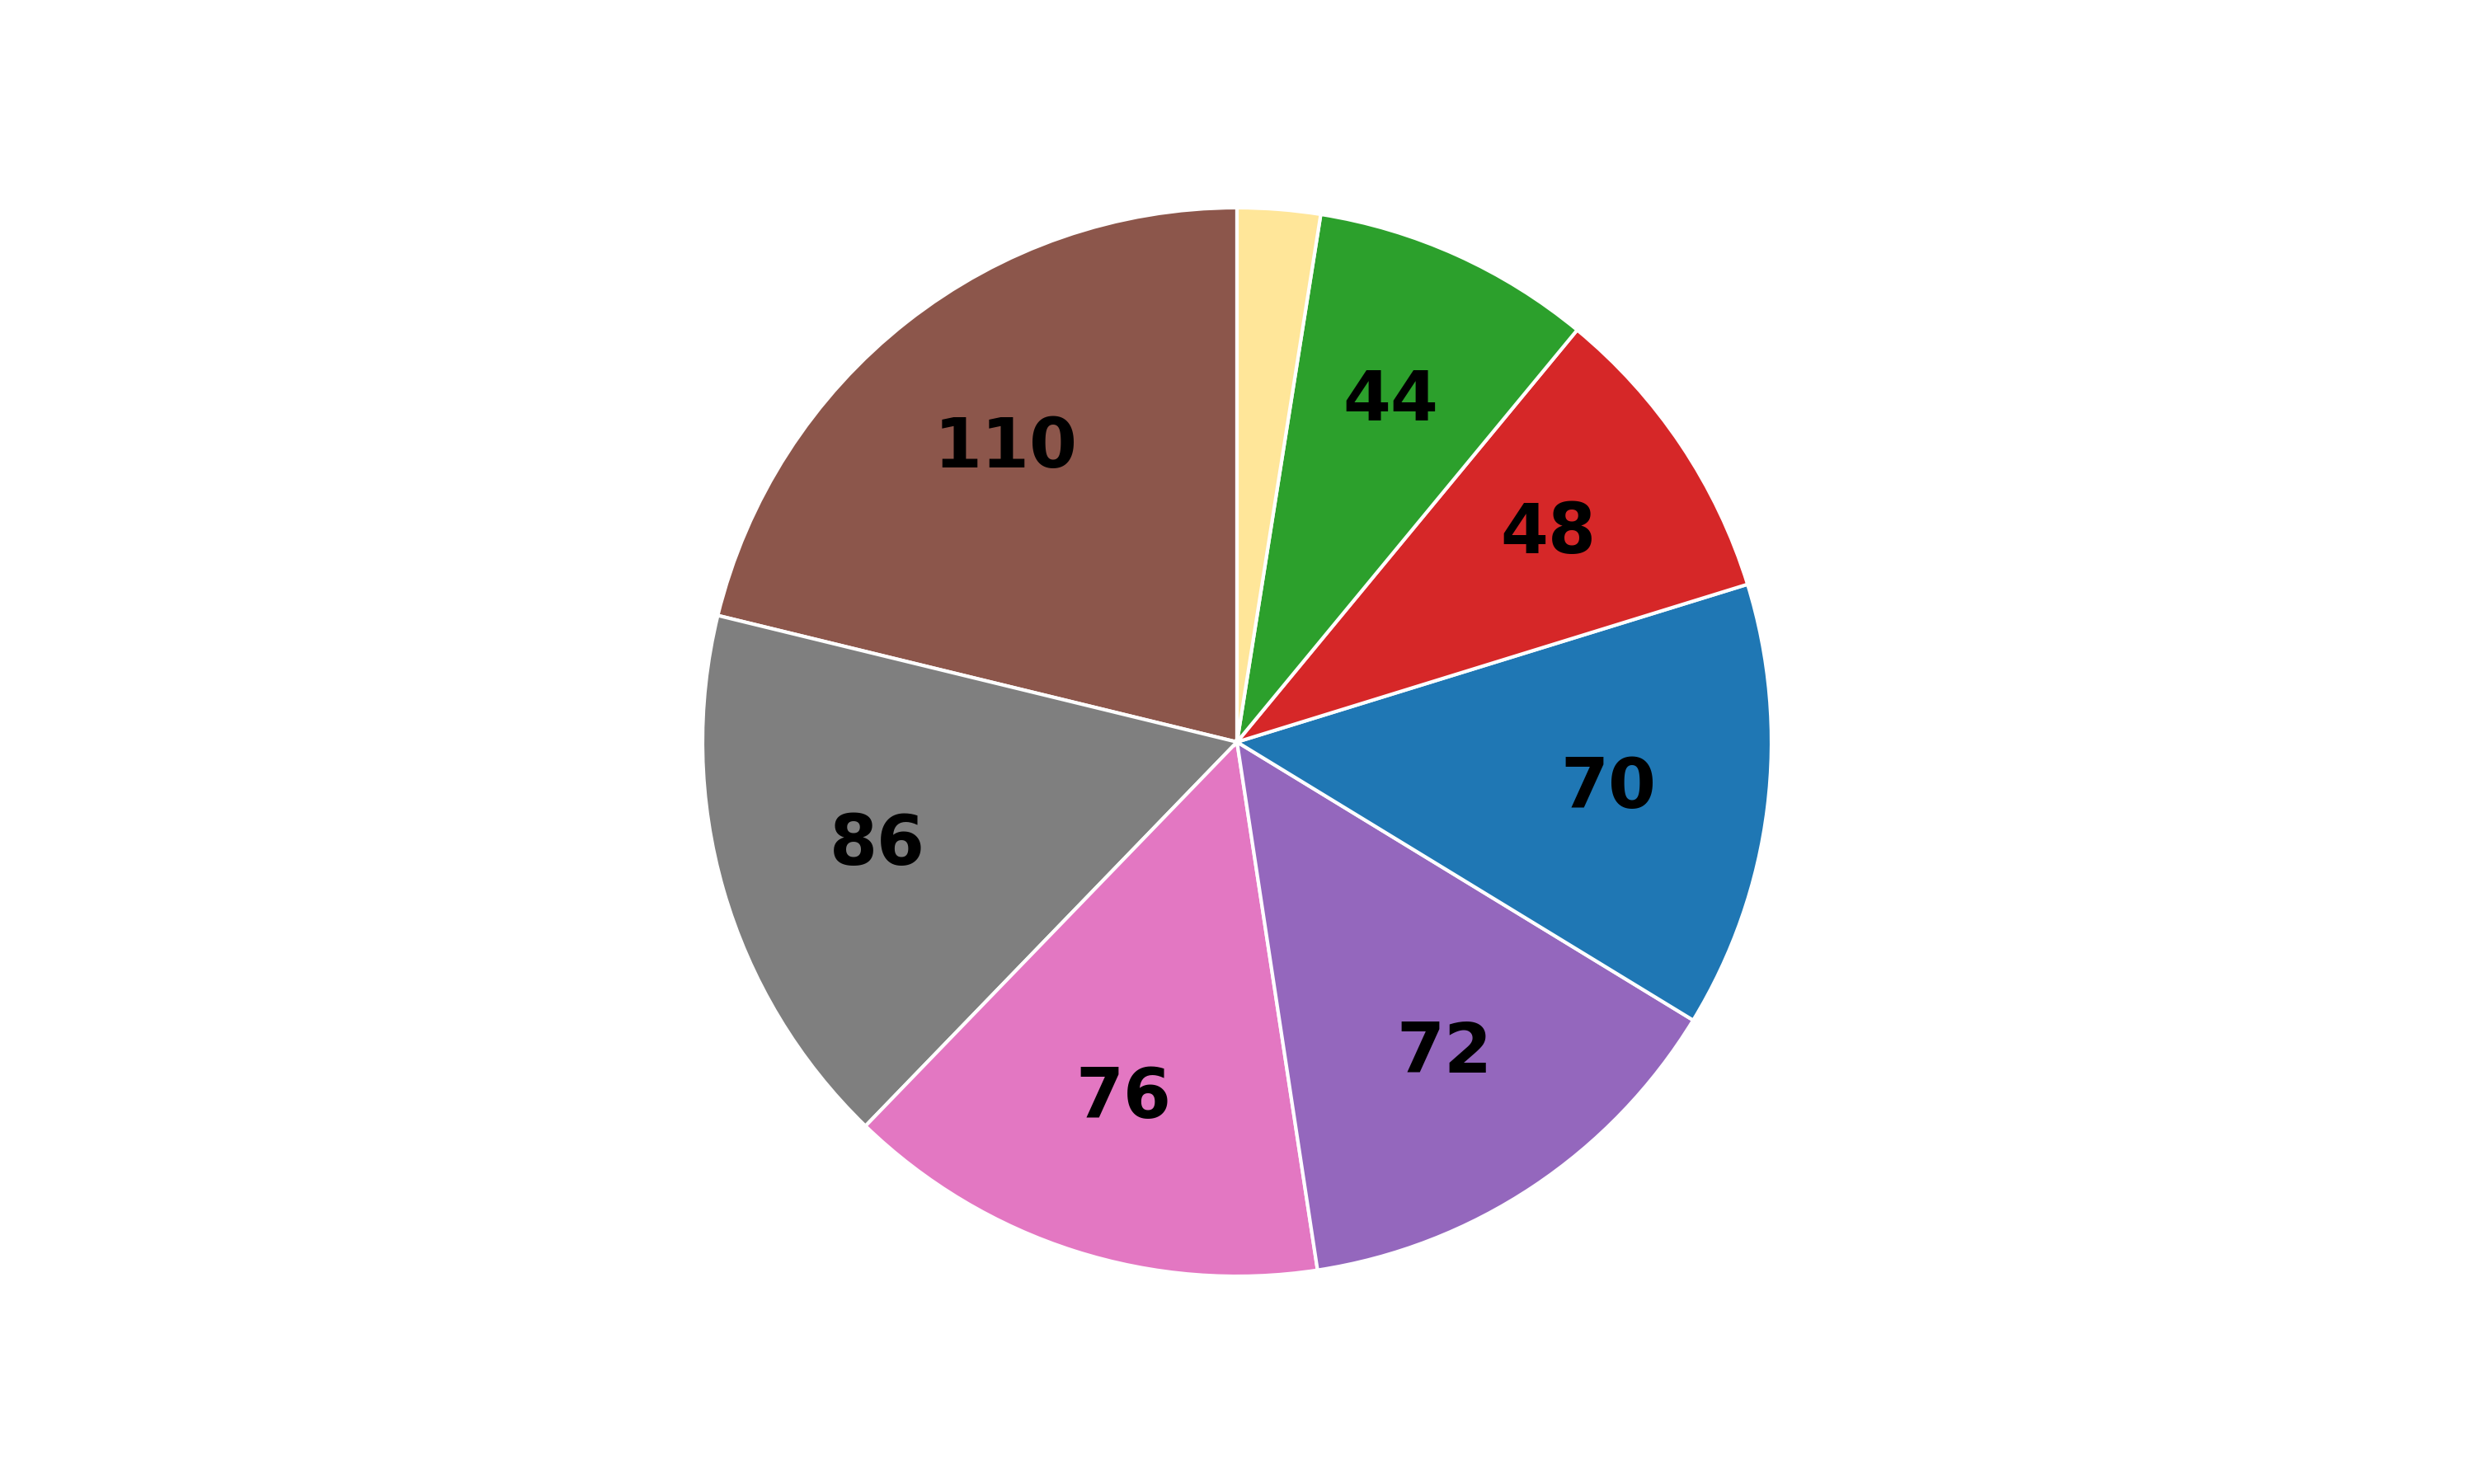
\includegraphics[width=0.45\textwidth]{figures/Un_0.3(PF)/0.8/pareto_contribution_piechart.png}
    }
    
    \subfloat[Traffic density = 0.9\label{fig:td1_c}]{
        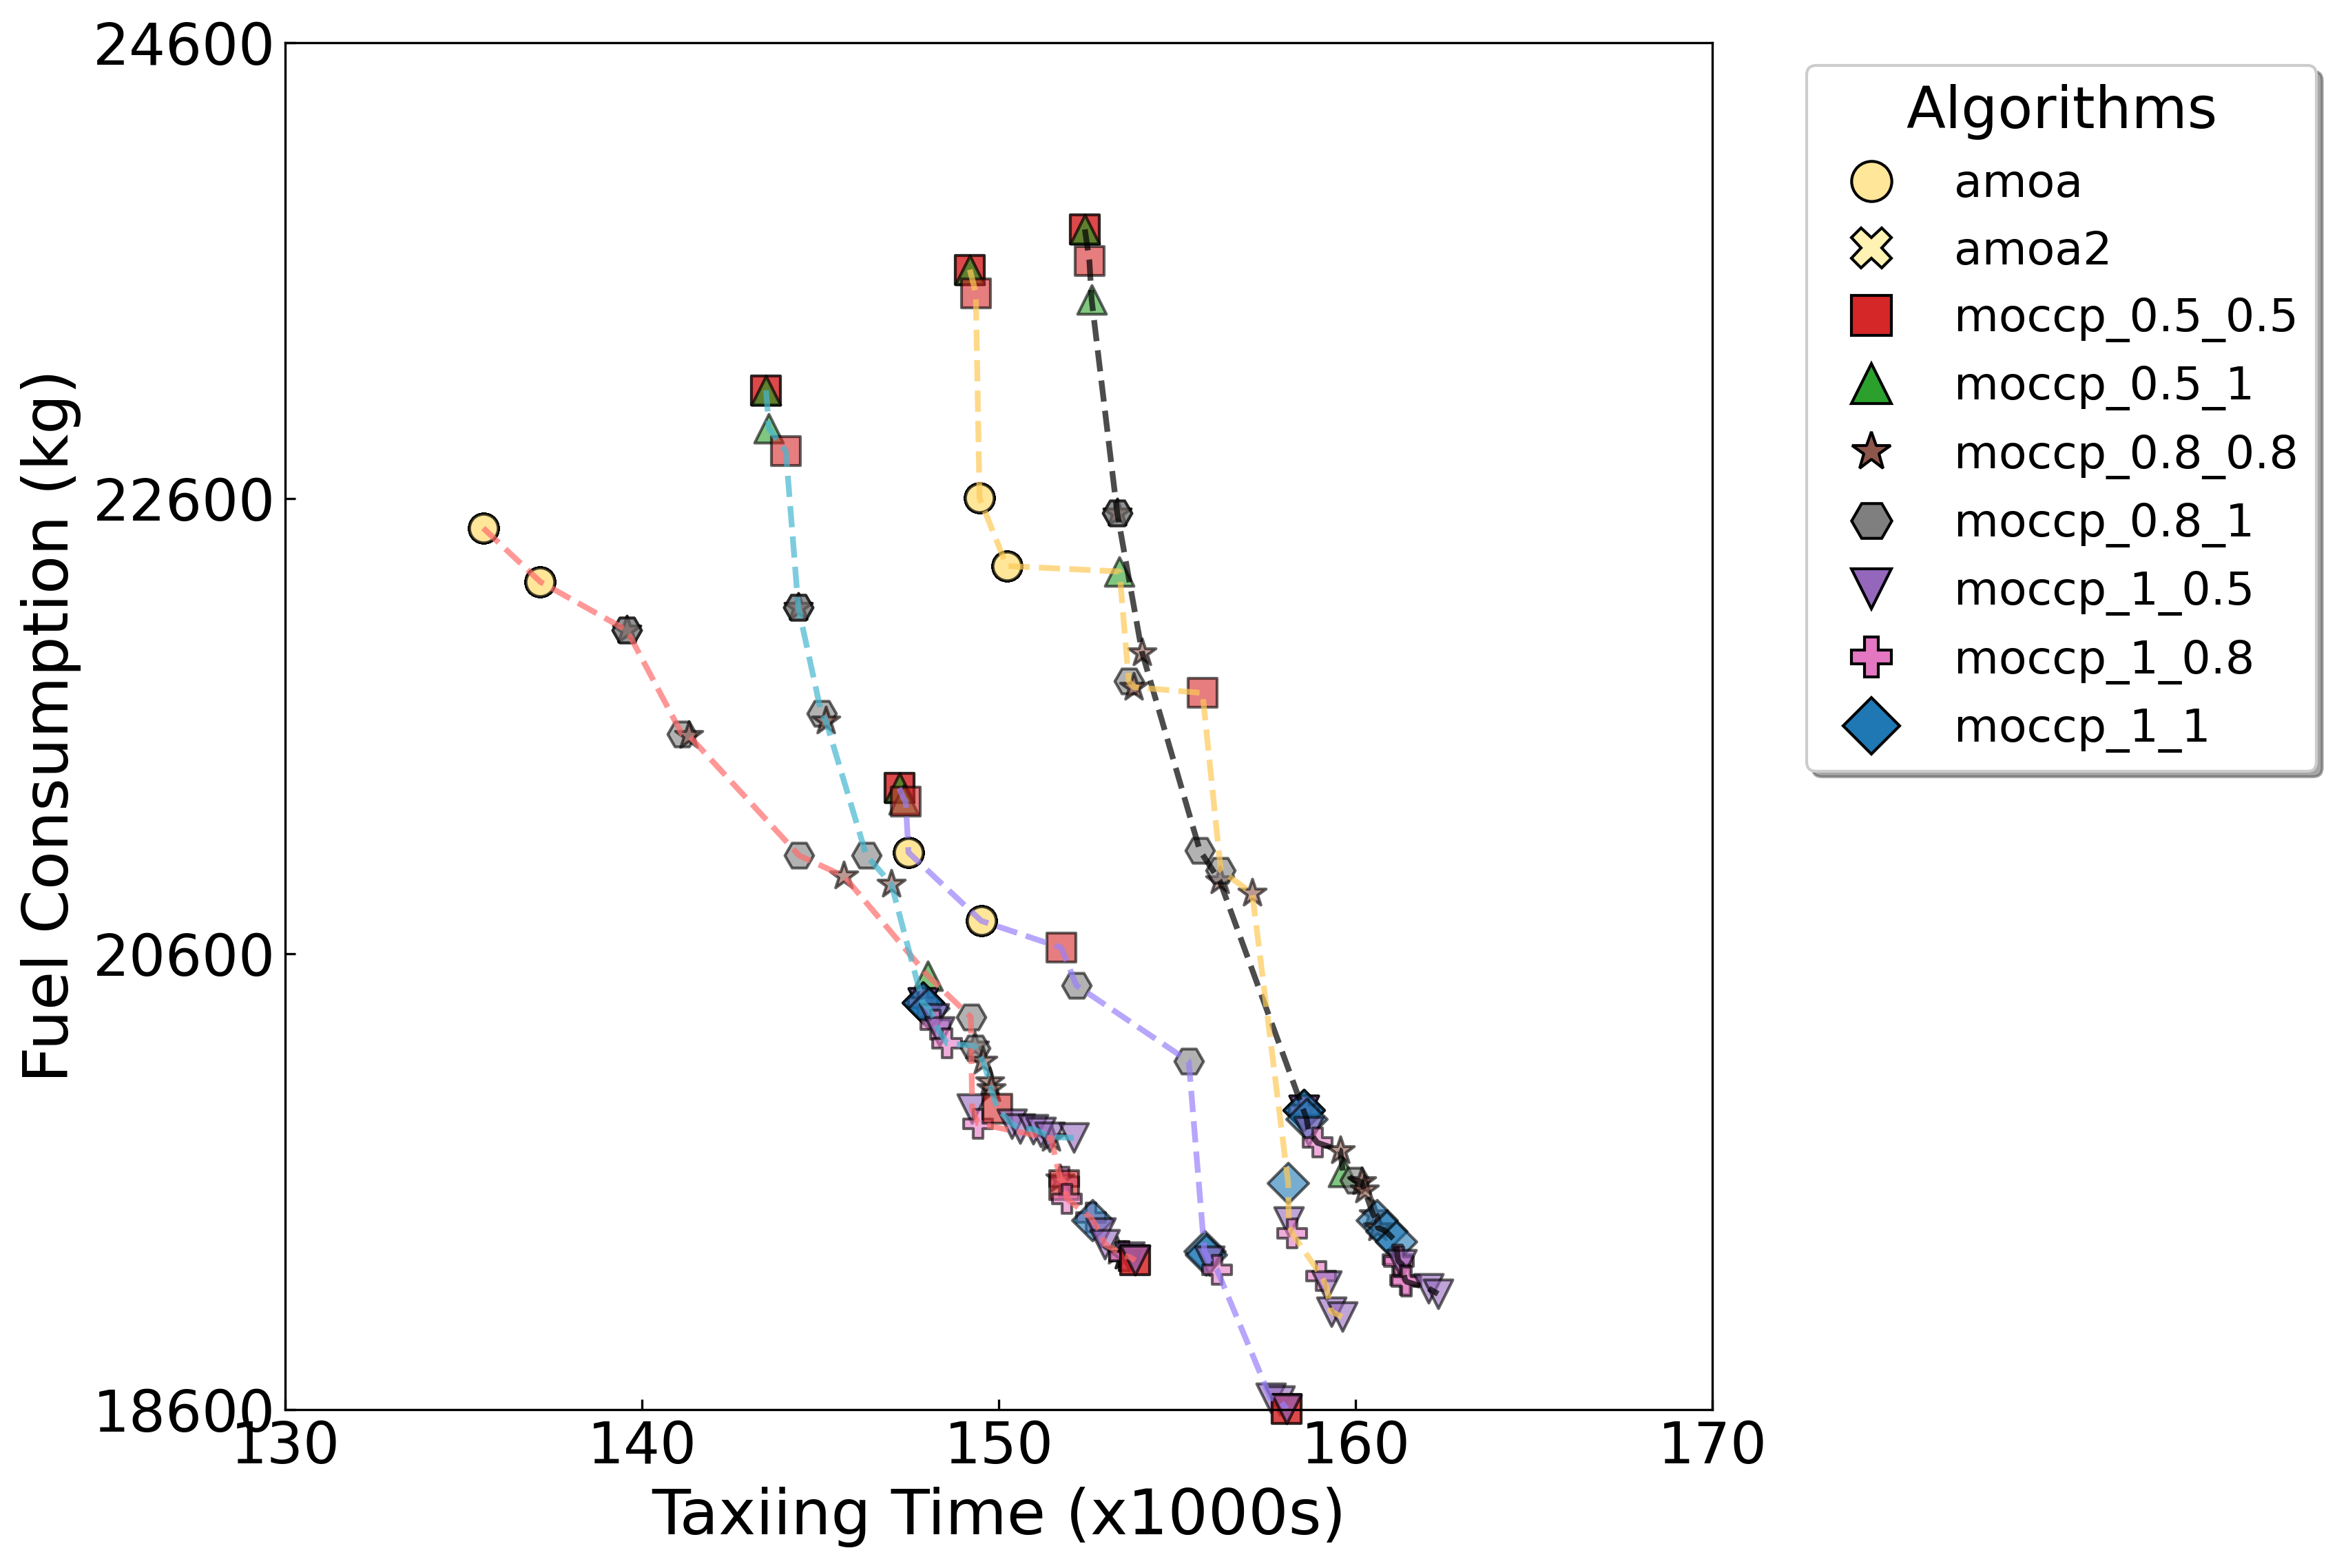
\includegraphics[width=0.45\textwidth]{figures/Un_0.3(PF)/0.9/pareto_fronts_colored.png}
    }
    \hspace{0.02\textwidth} 
    \subfloat[Traffic density = 0.9\label{fig:td1_d}]{
        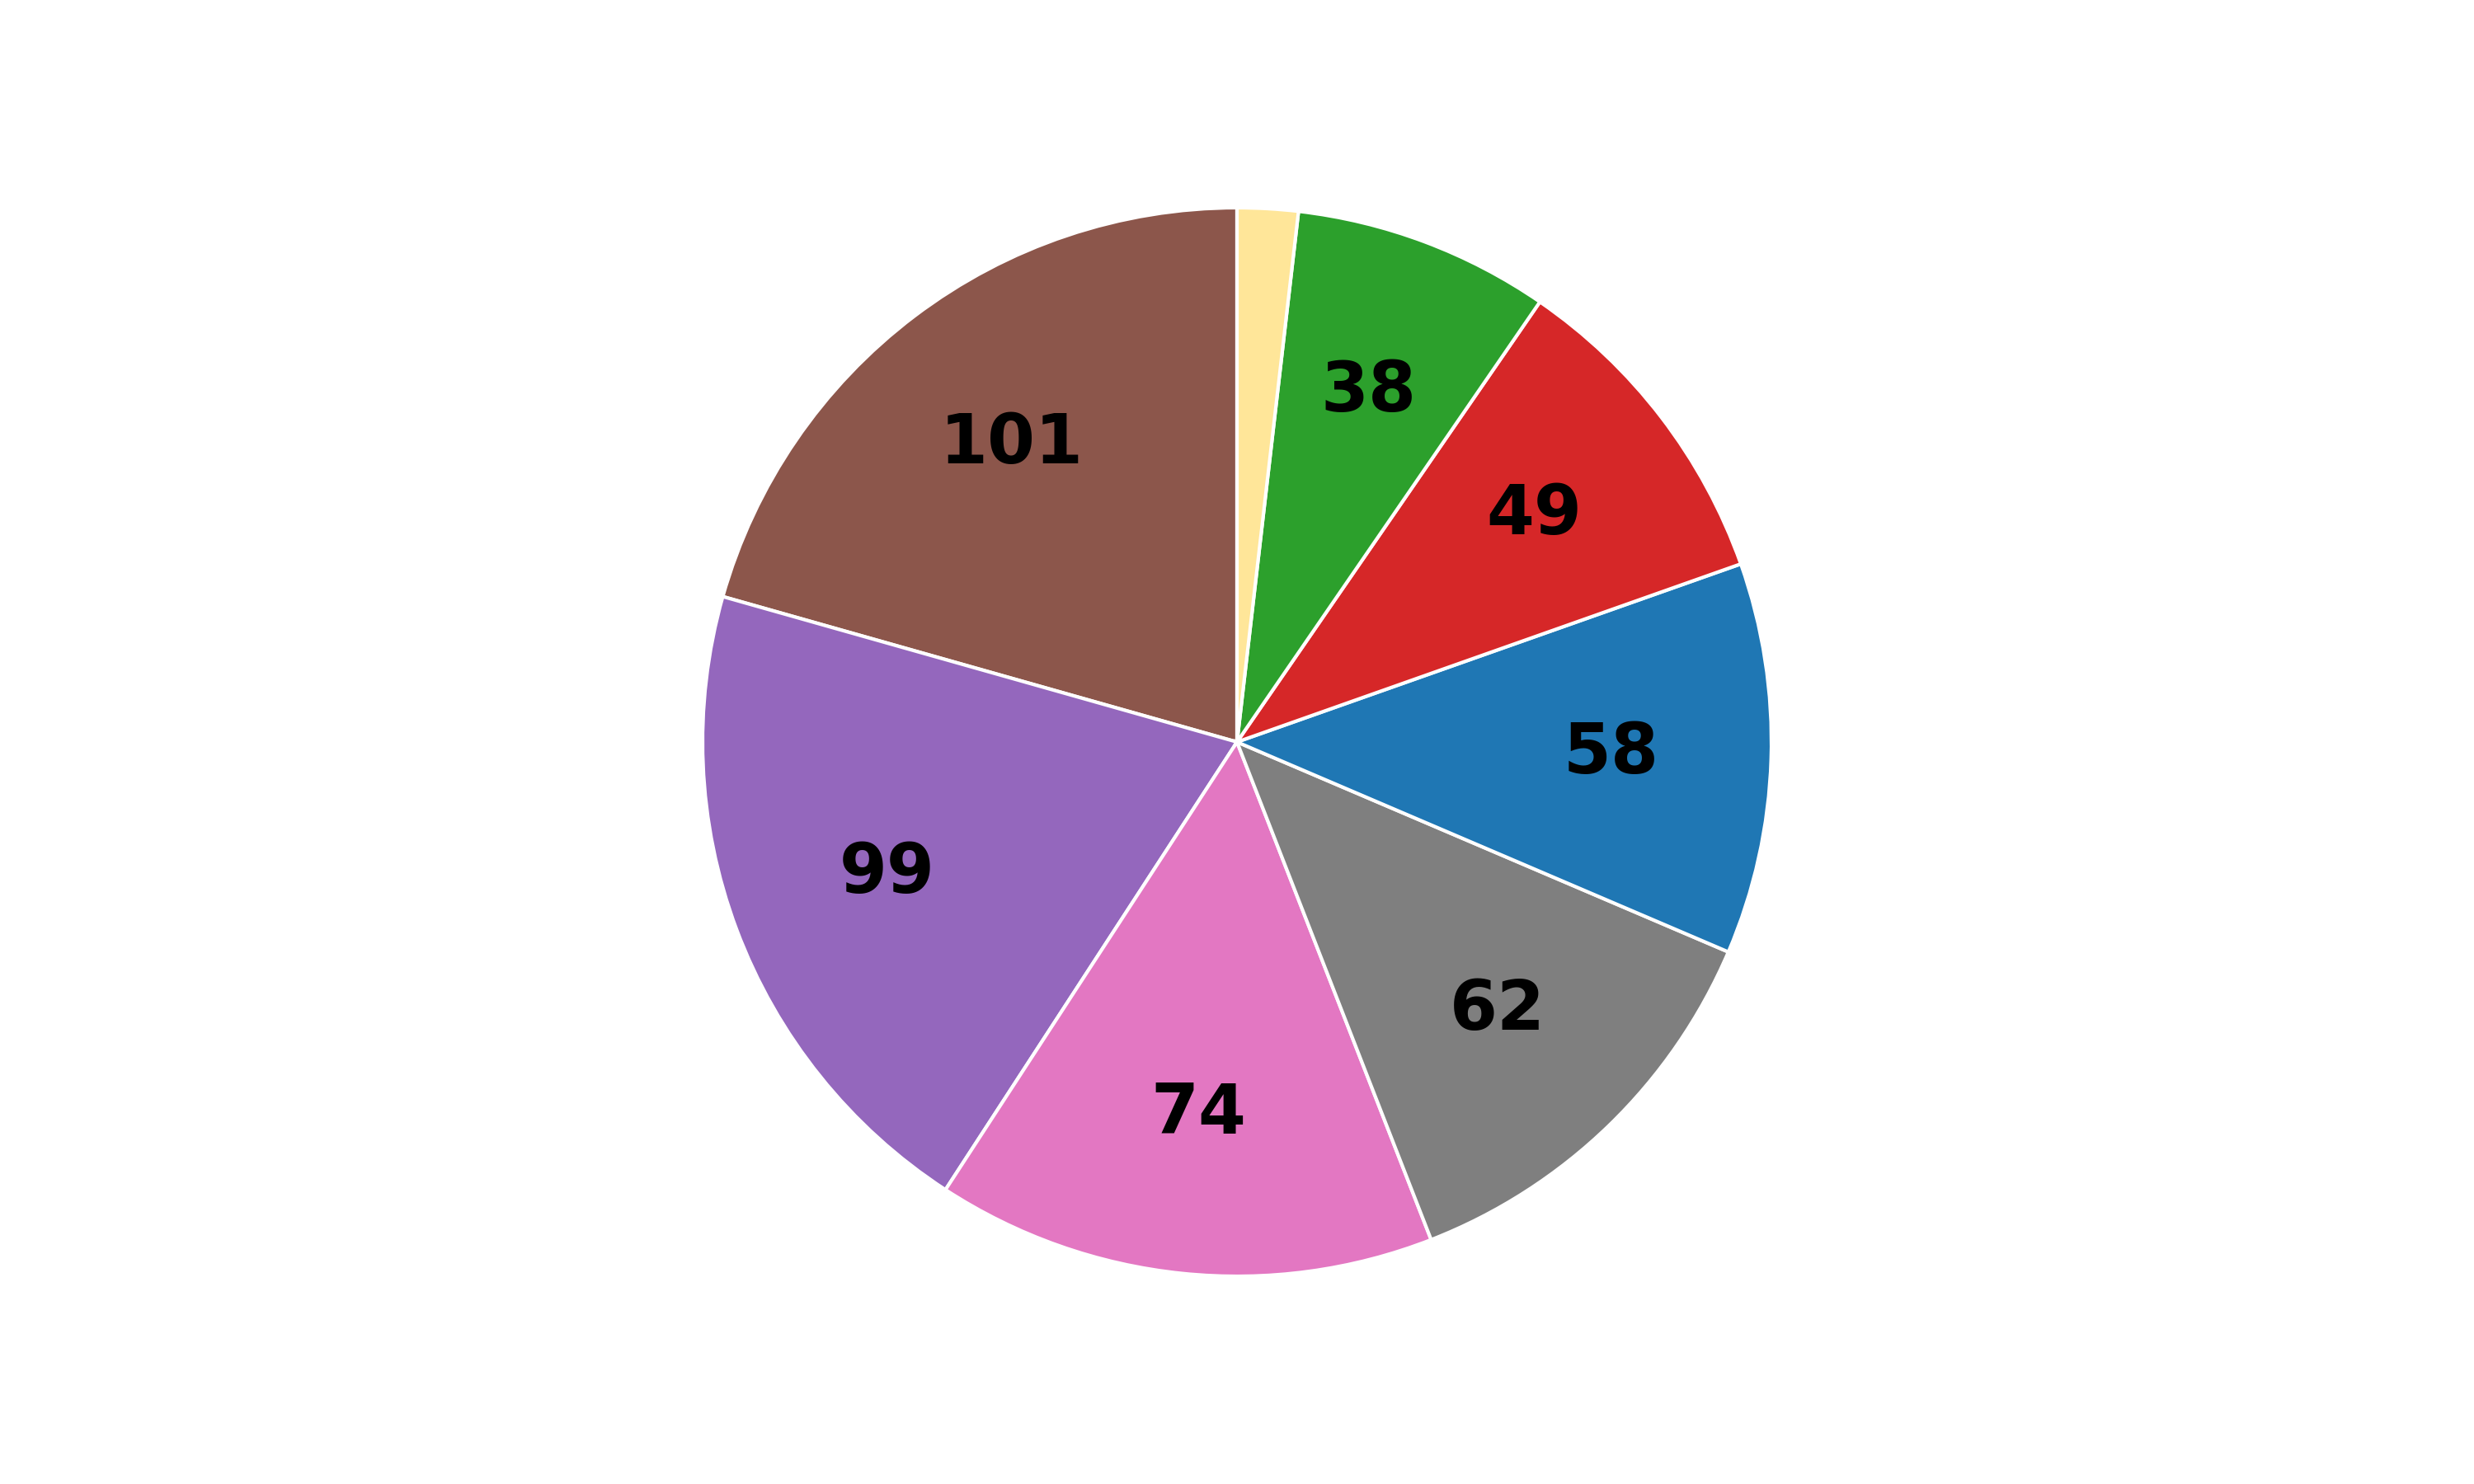
\includegraphics[width=0.45\textwidth]{figures/Un_0.3(PF)/0.9/pareto_contribution_piechart.png}
    }
    
    \subfloat[Traffic density = 1.0\label{fig:td1_e}]{
        \includegraphics[width=0.45\textwidth]{figures/Un_0.3(PF)/1.0/pareto_fronts_colored.png}
    }
    \hspace{0.02\textwidth} 
    \subfloat[Traffic density = 1.0\label{fig:td1_f}]{
        \includegraphics[width=0.45\textwidth]{figures/Un_0.3(PF)/1.0/pareto_contribution_piechart.png}
    }
    
    \caption{Pareto fronts (5 simulations) along with statistics of flimsily robust efficient points (30 simulations) at uncertainty level 0.3 across different traffic densities. \blue{Each Pareto Front is extracted from the combined solutions of all algorithms in each simulation.} Colour-algorithm associations in pie charts match the Pareto front legends. For example, the pink segment in (f) indicates \texttt{moccp\_1\_0.8} produced 66 robust points.}
    \label{fig:td1}
\end{figure}

\begin{figure}[htp]
    \centering
    
    \subfloat[Pareto fronts for density 1.1\label{fig:td2_g}]{
        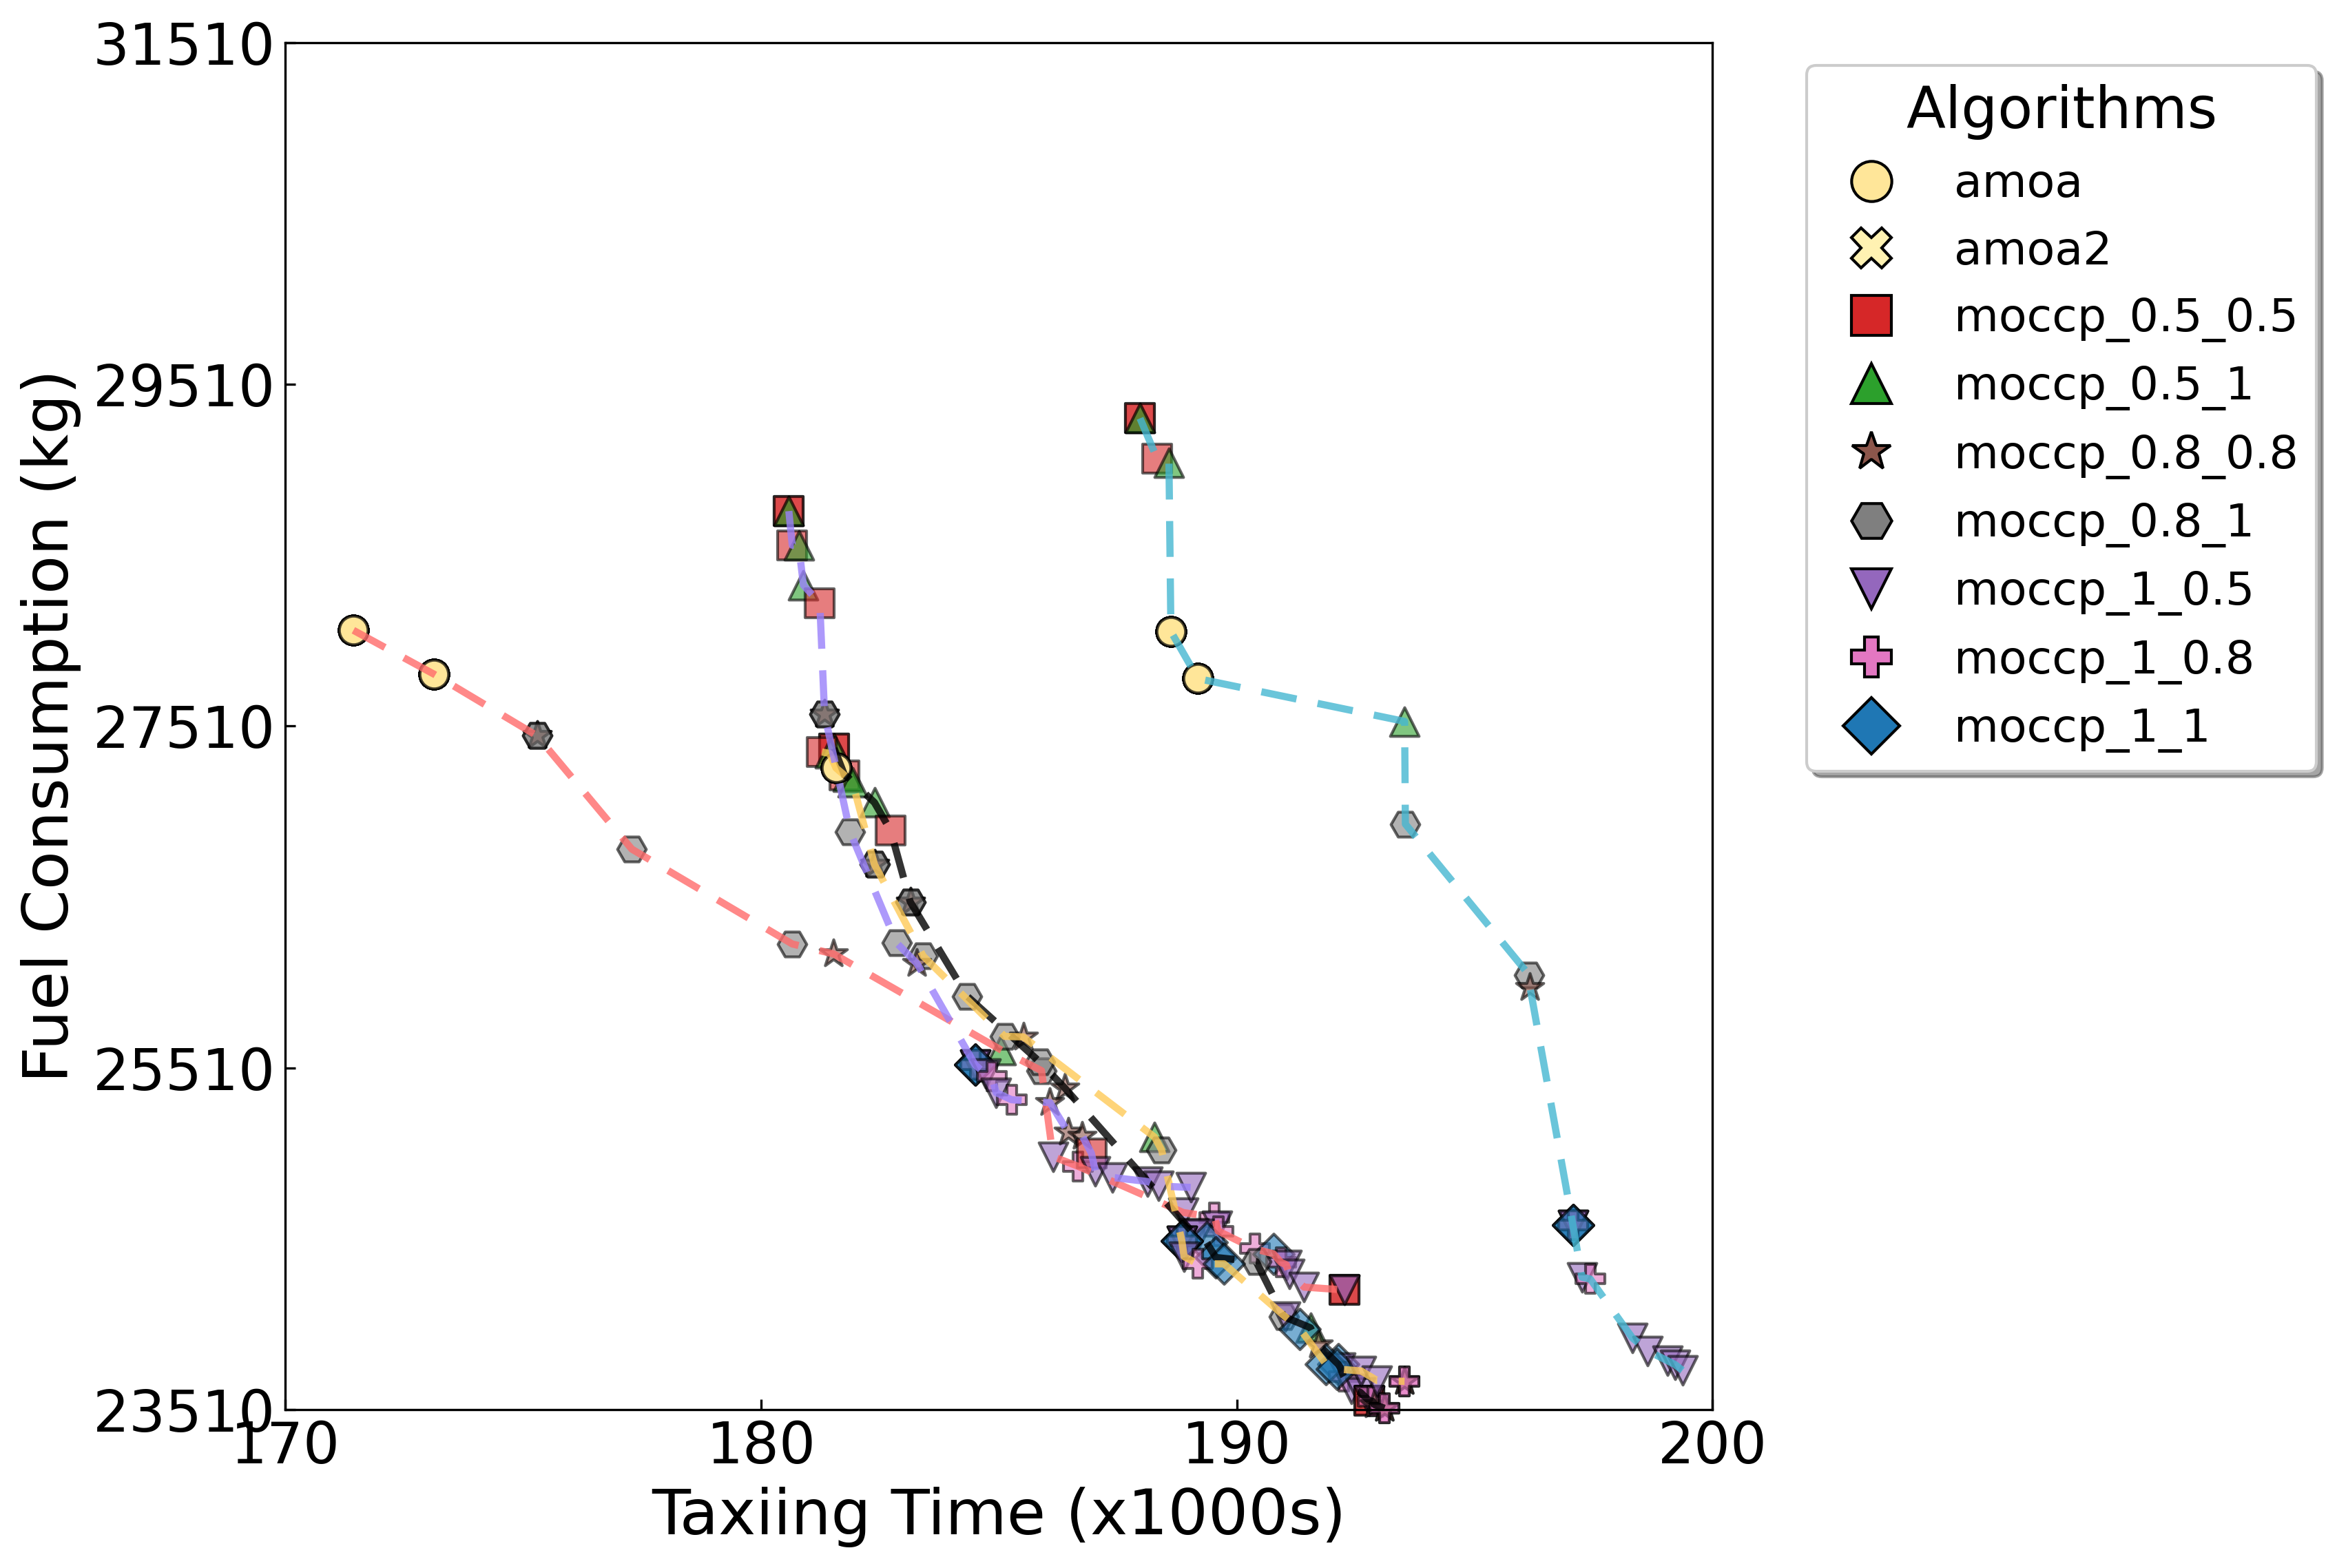
\includegraphics[width=0.45\textwidth]{figures/Un_0.3(PF)/1.1/pareto_fronts_colored.png}
    }
    \hspace{0.02\textwidth} 
    \subfloat[Pie chart for density 1.1\label{fig:td2_h}]{
        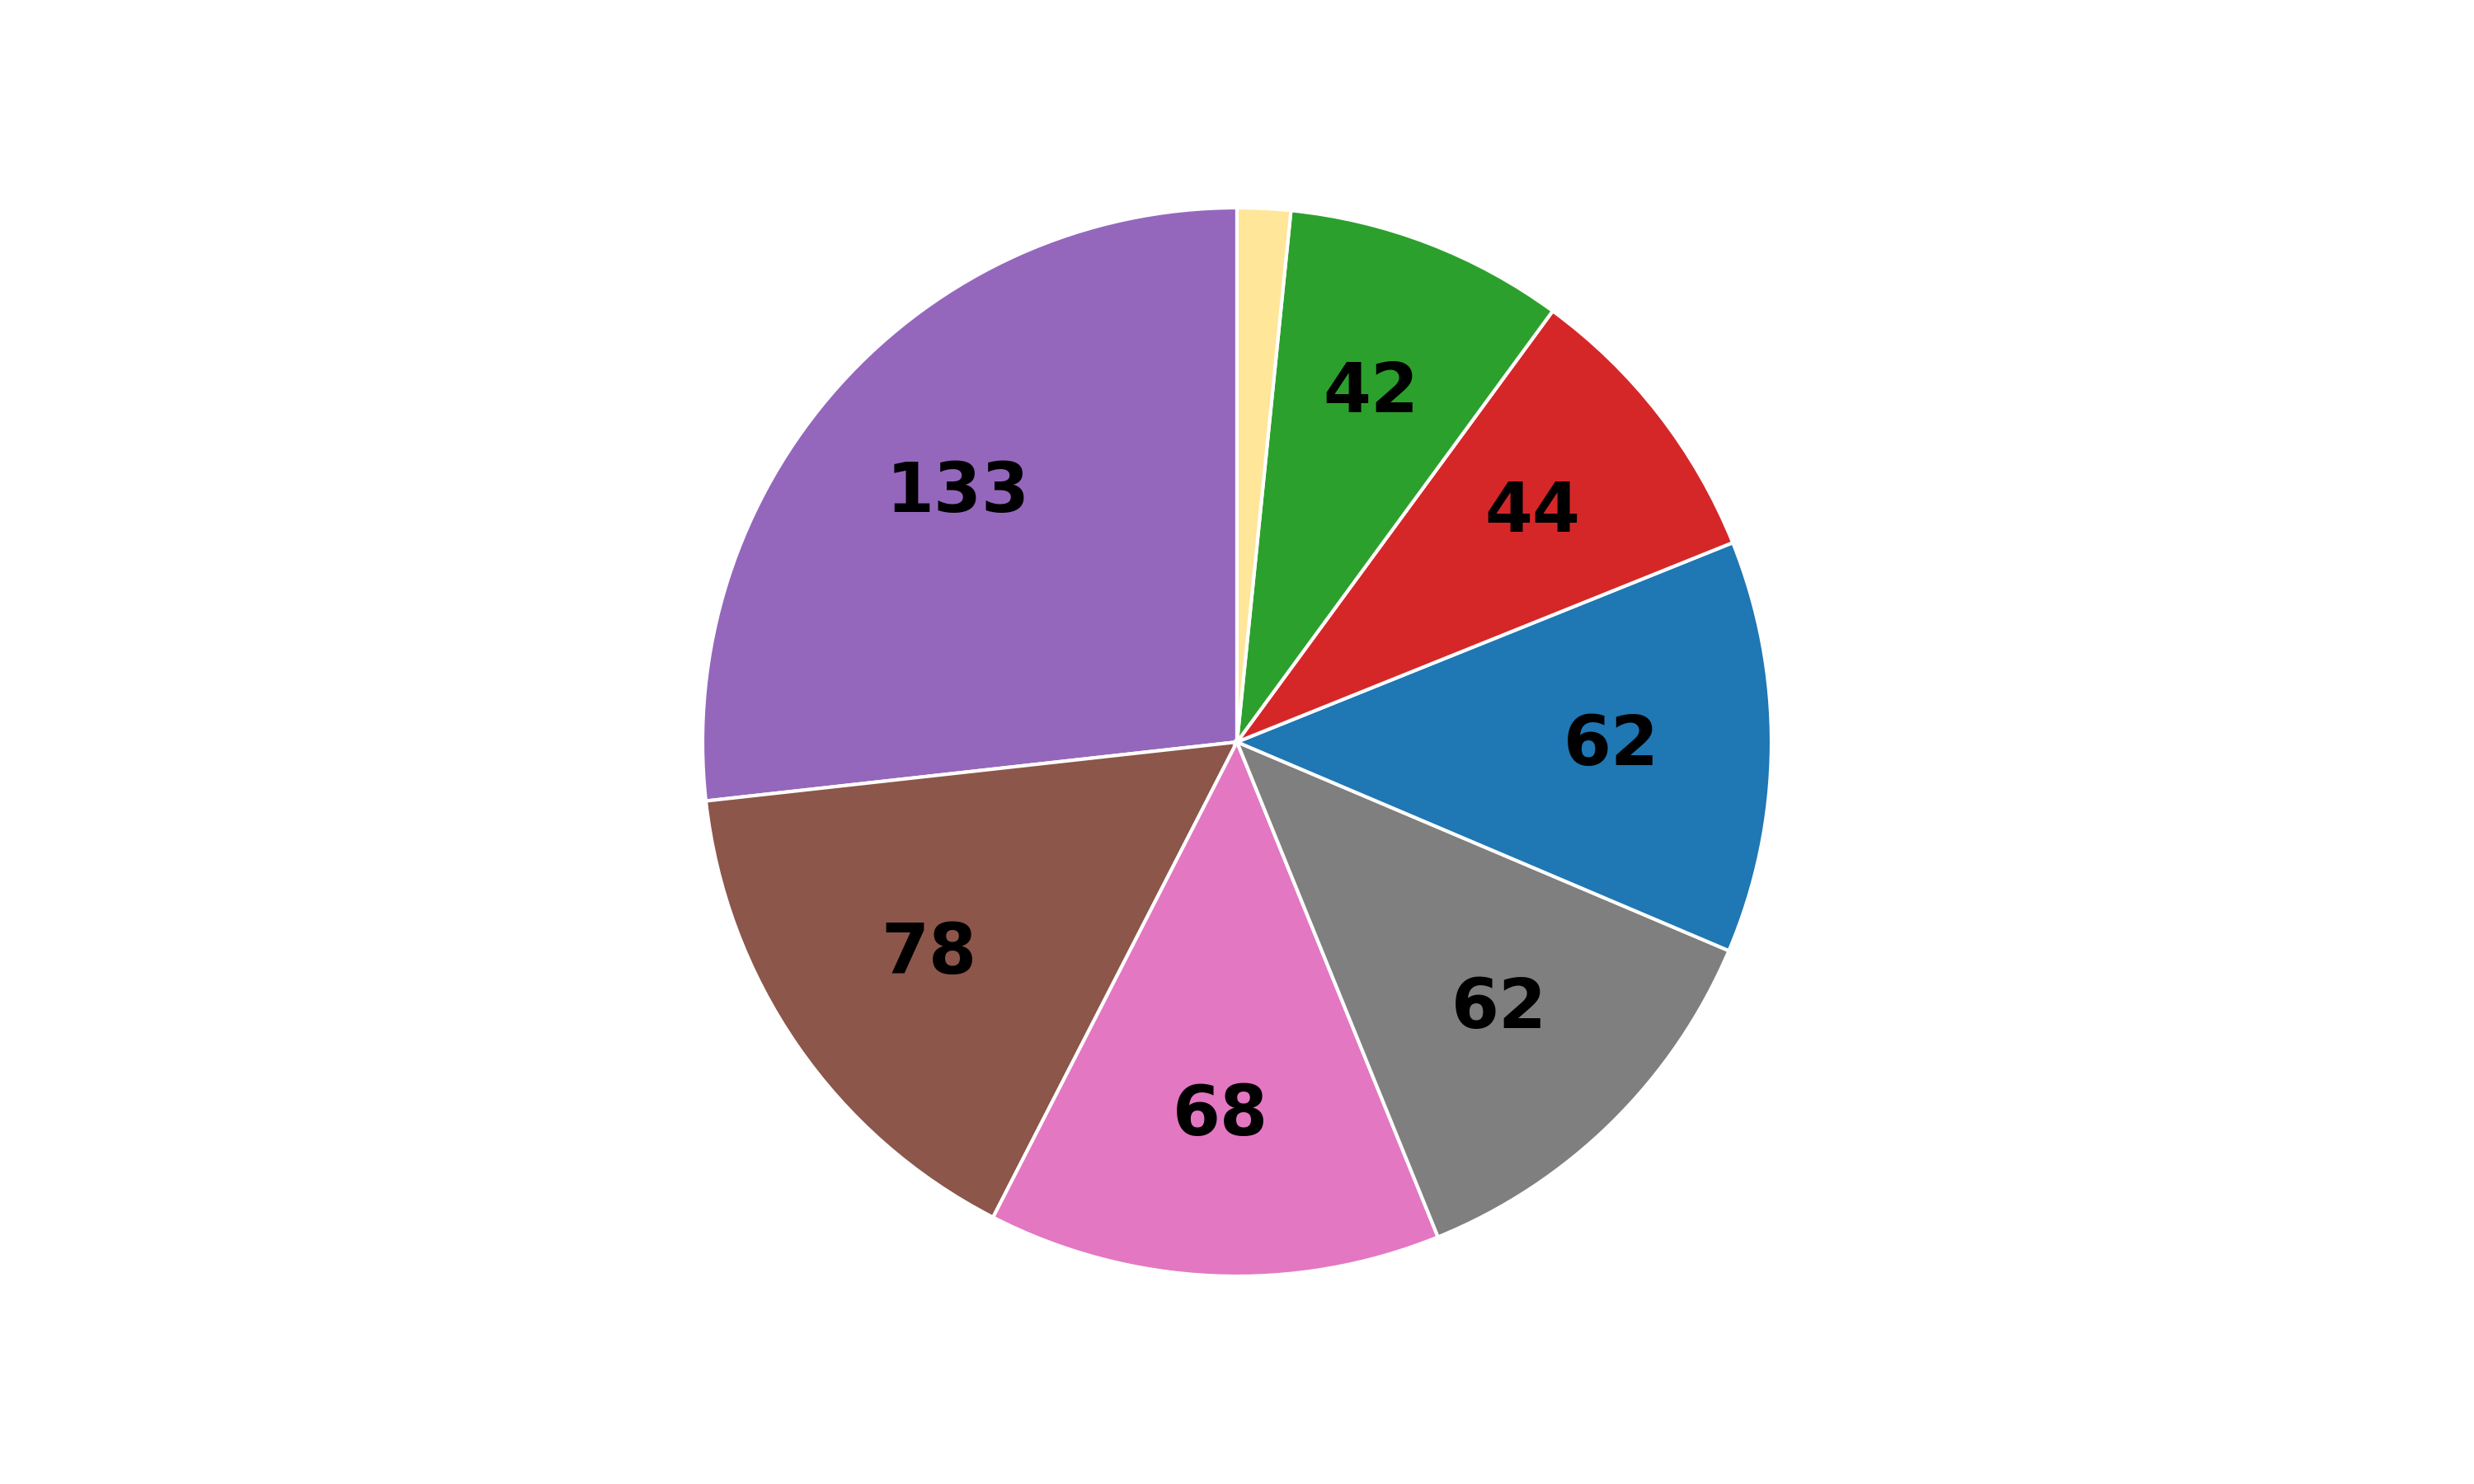
\includegraphics[width=0.45\textwidth]{figures/Un_0.3(PF)/1.1/pareto_contribution_piechart.png}
    }
    
    \subfloat[Pareto fronts for density 1.2\label{fig:td2_i}]{
        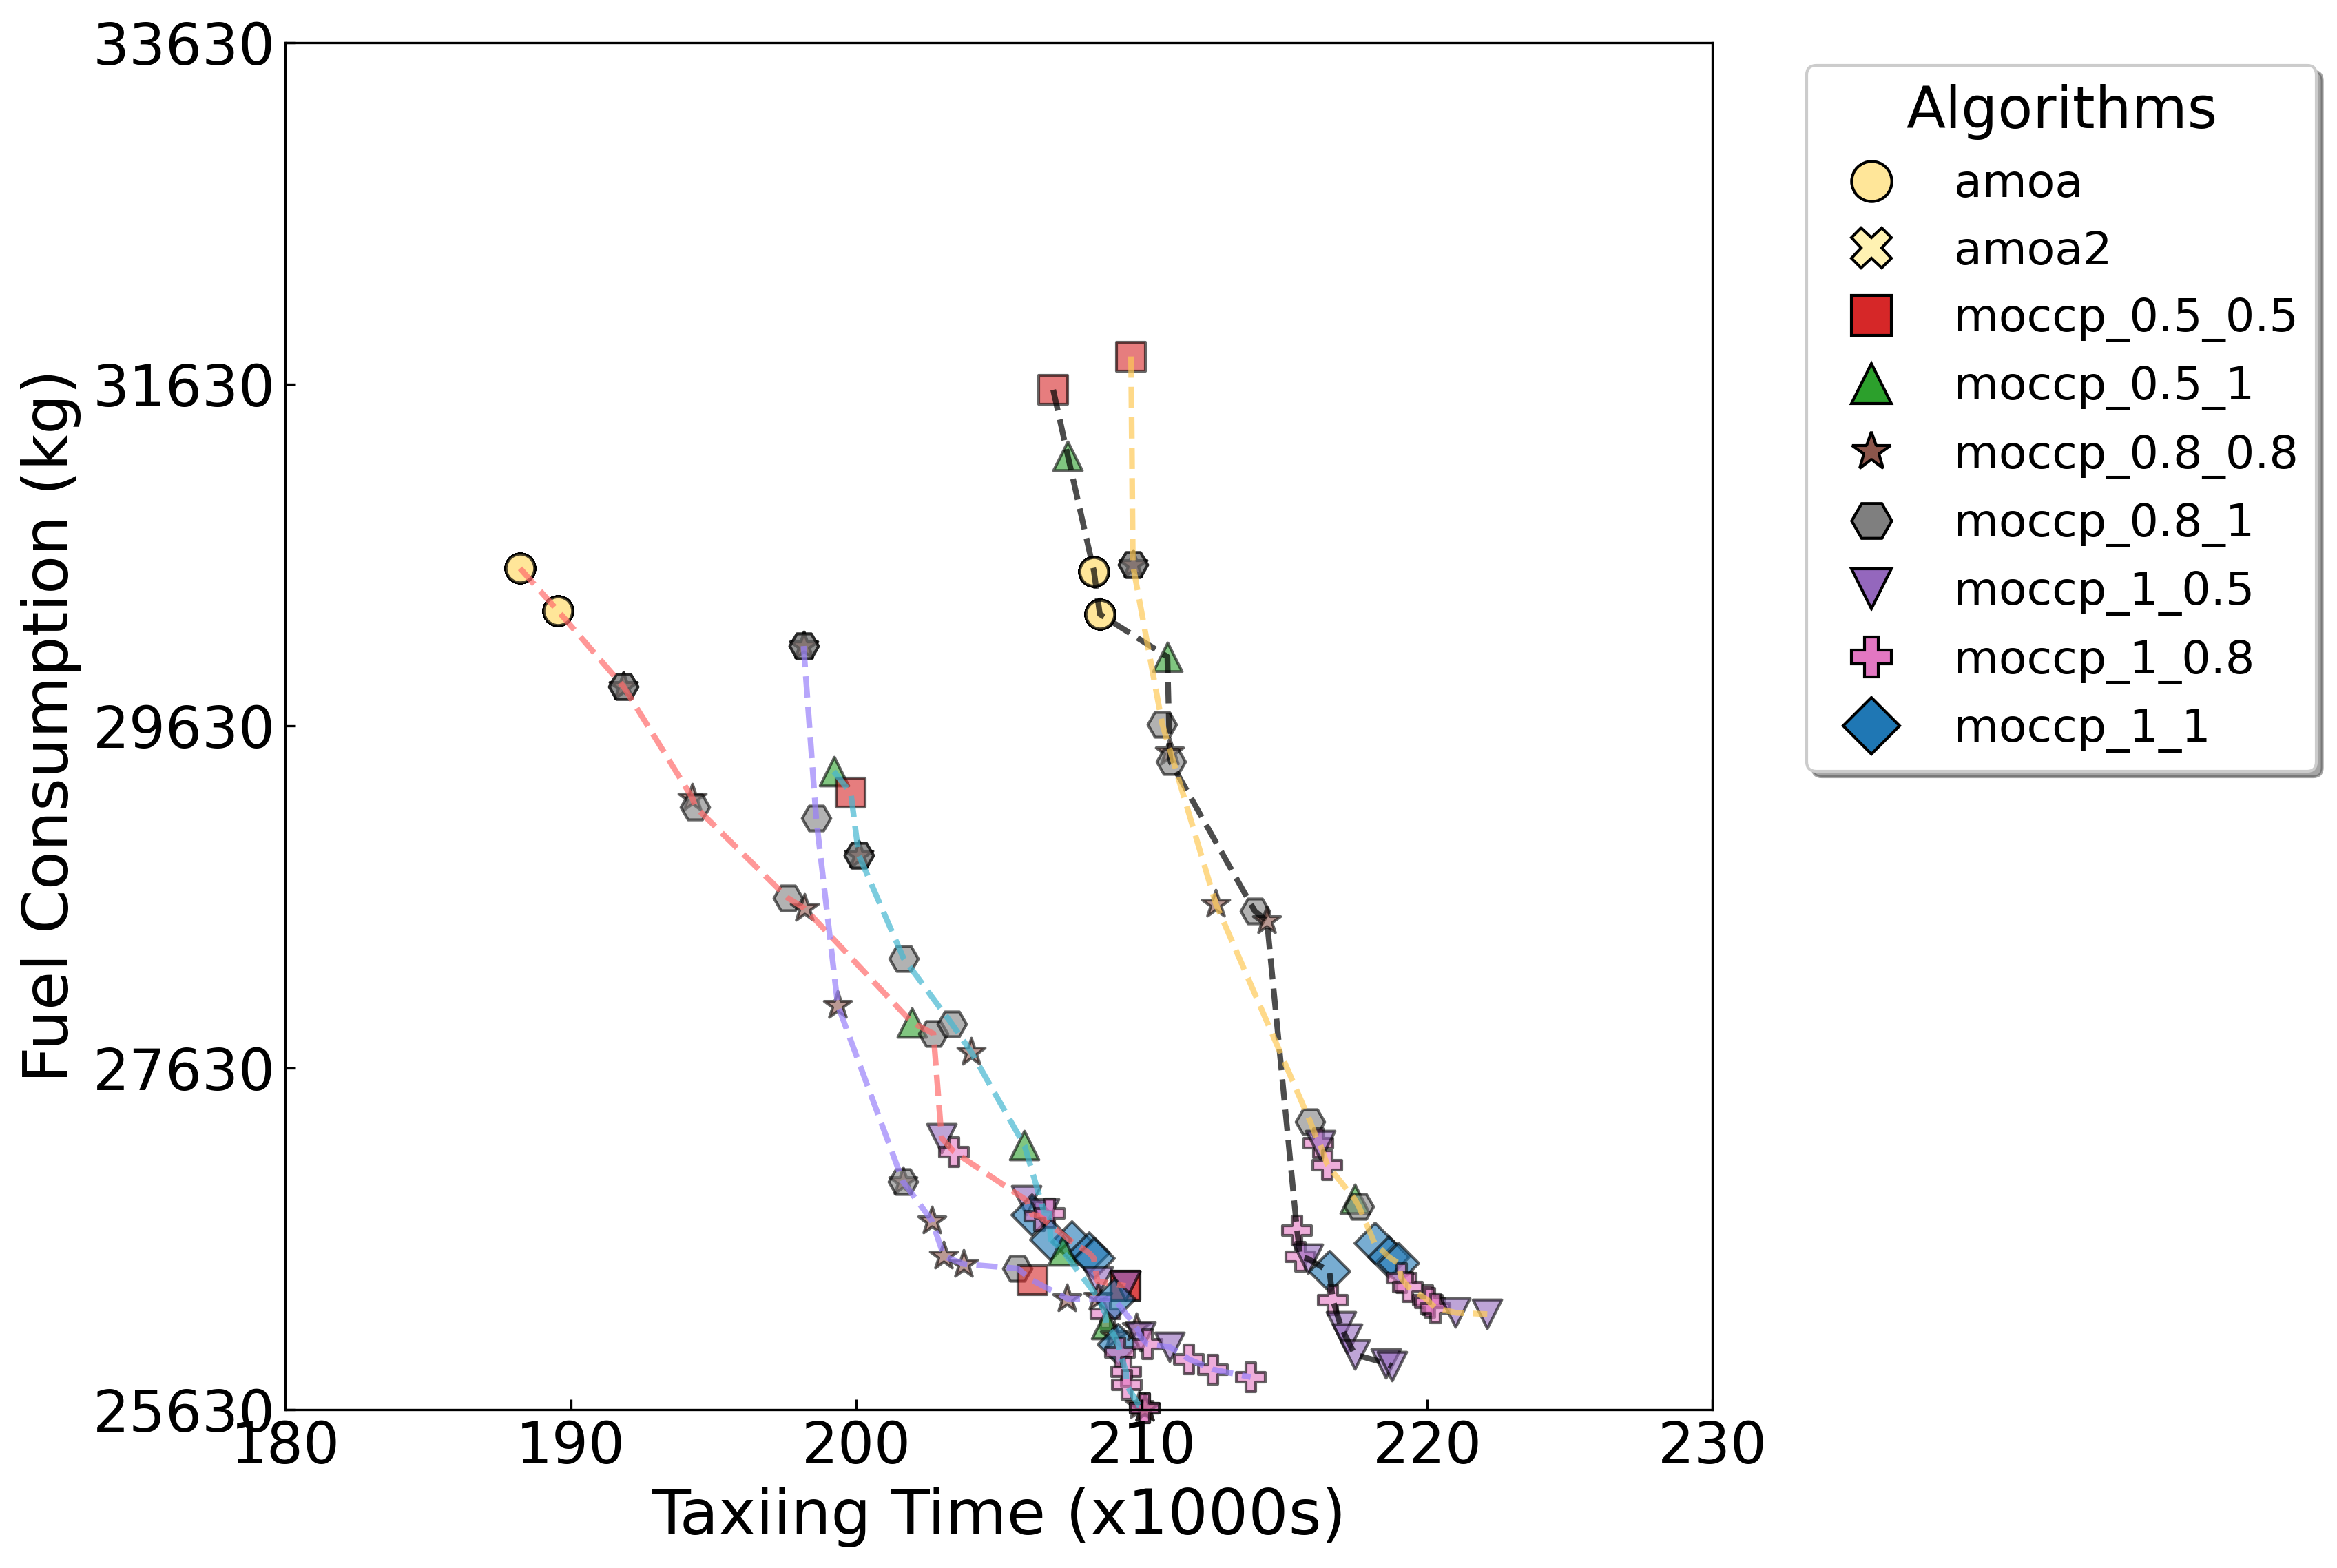
\includegraphics[width=0.45\textwidth]{figures/Un_0.3(PF)/1.2/pareto_fronts_colored.png}
    }
    \hspace{0.02\textwidth} 
    \subfloat[Pie chart for density 1.2\label{fig:td2_j}]{
        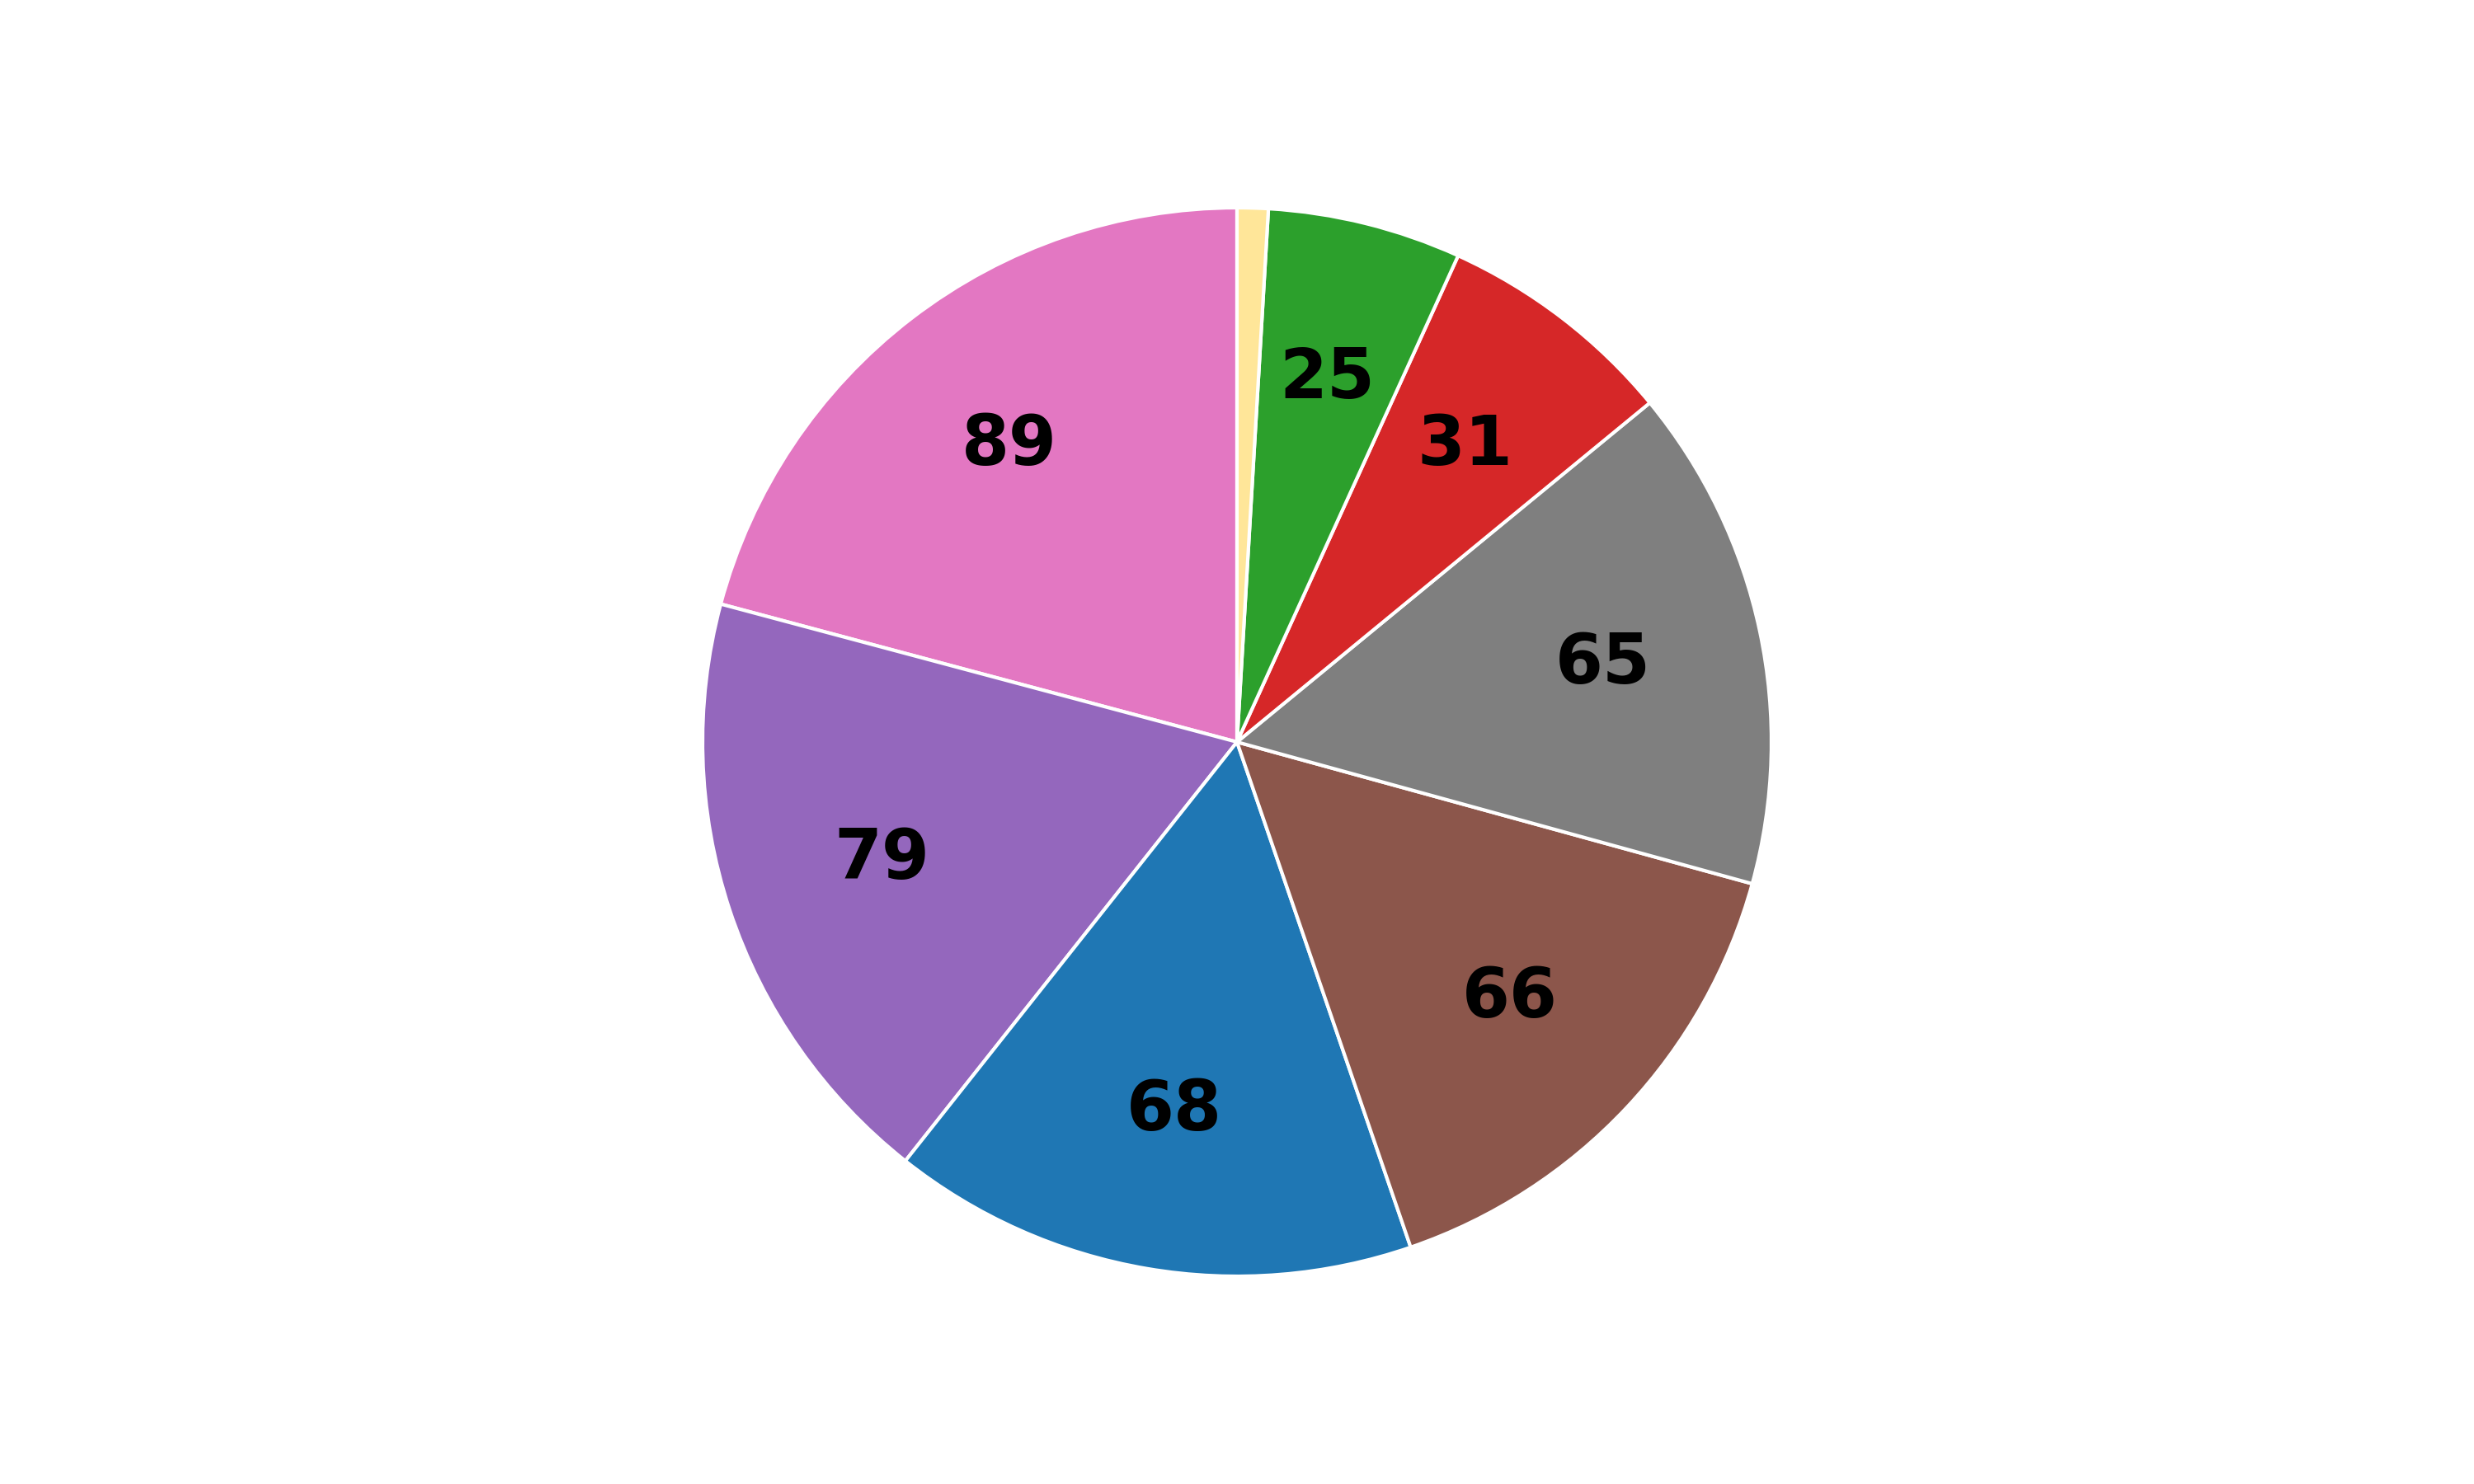
\includegraphics[width=0.45\textwidth]{figures/Un_0.3(PF)/1.2/pareto_contribution_piechart.png}
    }
    
    \caption{Pareto fronts (5 simulations) along with the statistics of flimsily robust efficient points (30 simulations) at uncertainty level 0.3 across different traffic densities.}
    \label{fig:td2}
\end{figure}

\begin{figure}[htp]
    \centering
    
    % Row 1: Uncertainty 0.1
    \subfloat[Uncertainty level = 0.1\label{fig:un_a}]{
        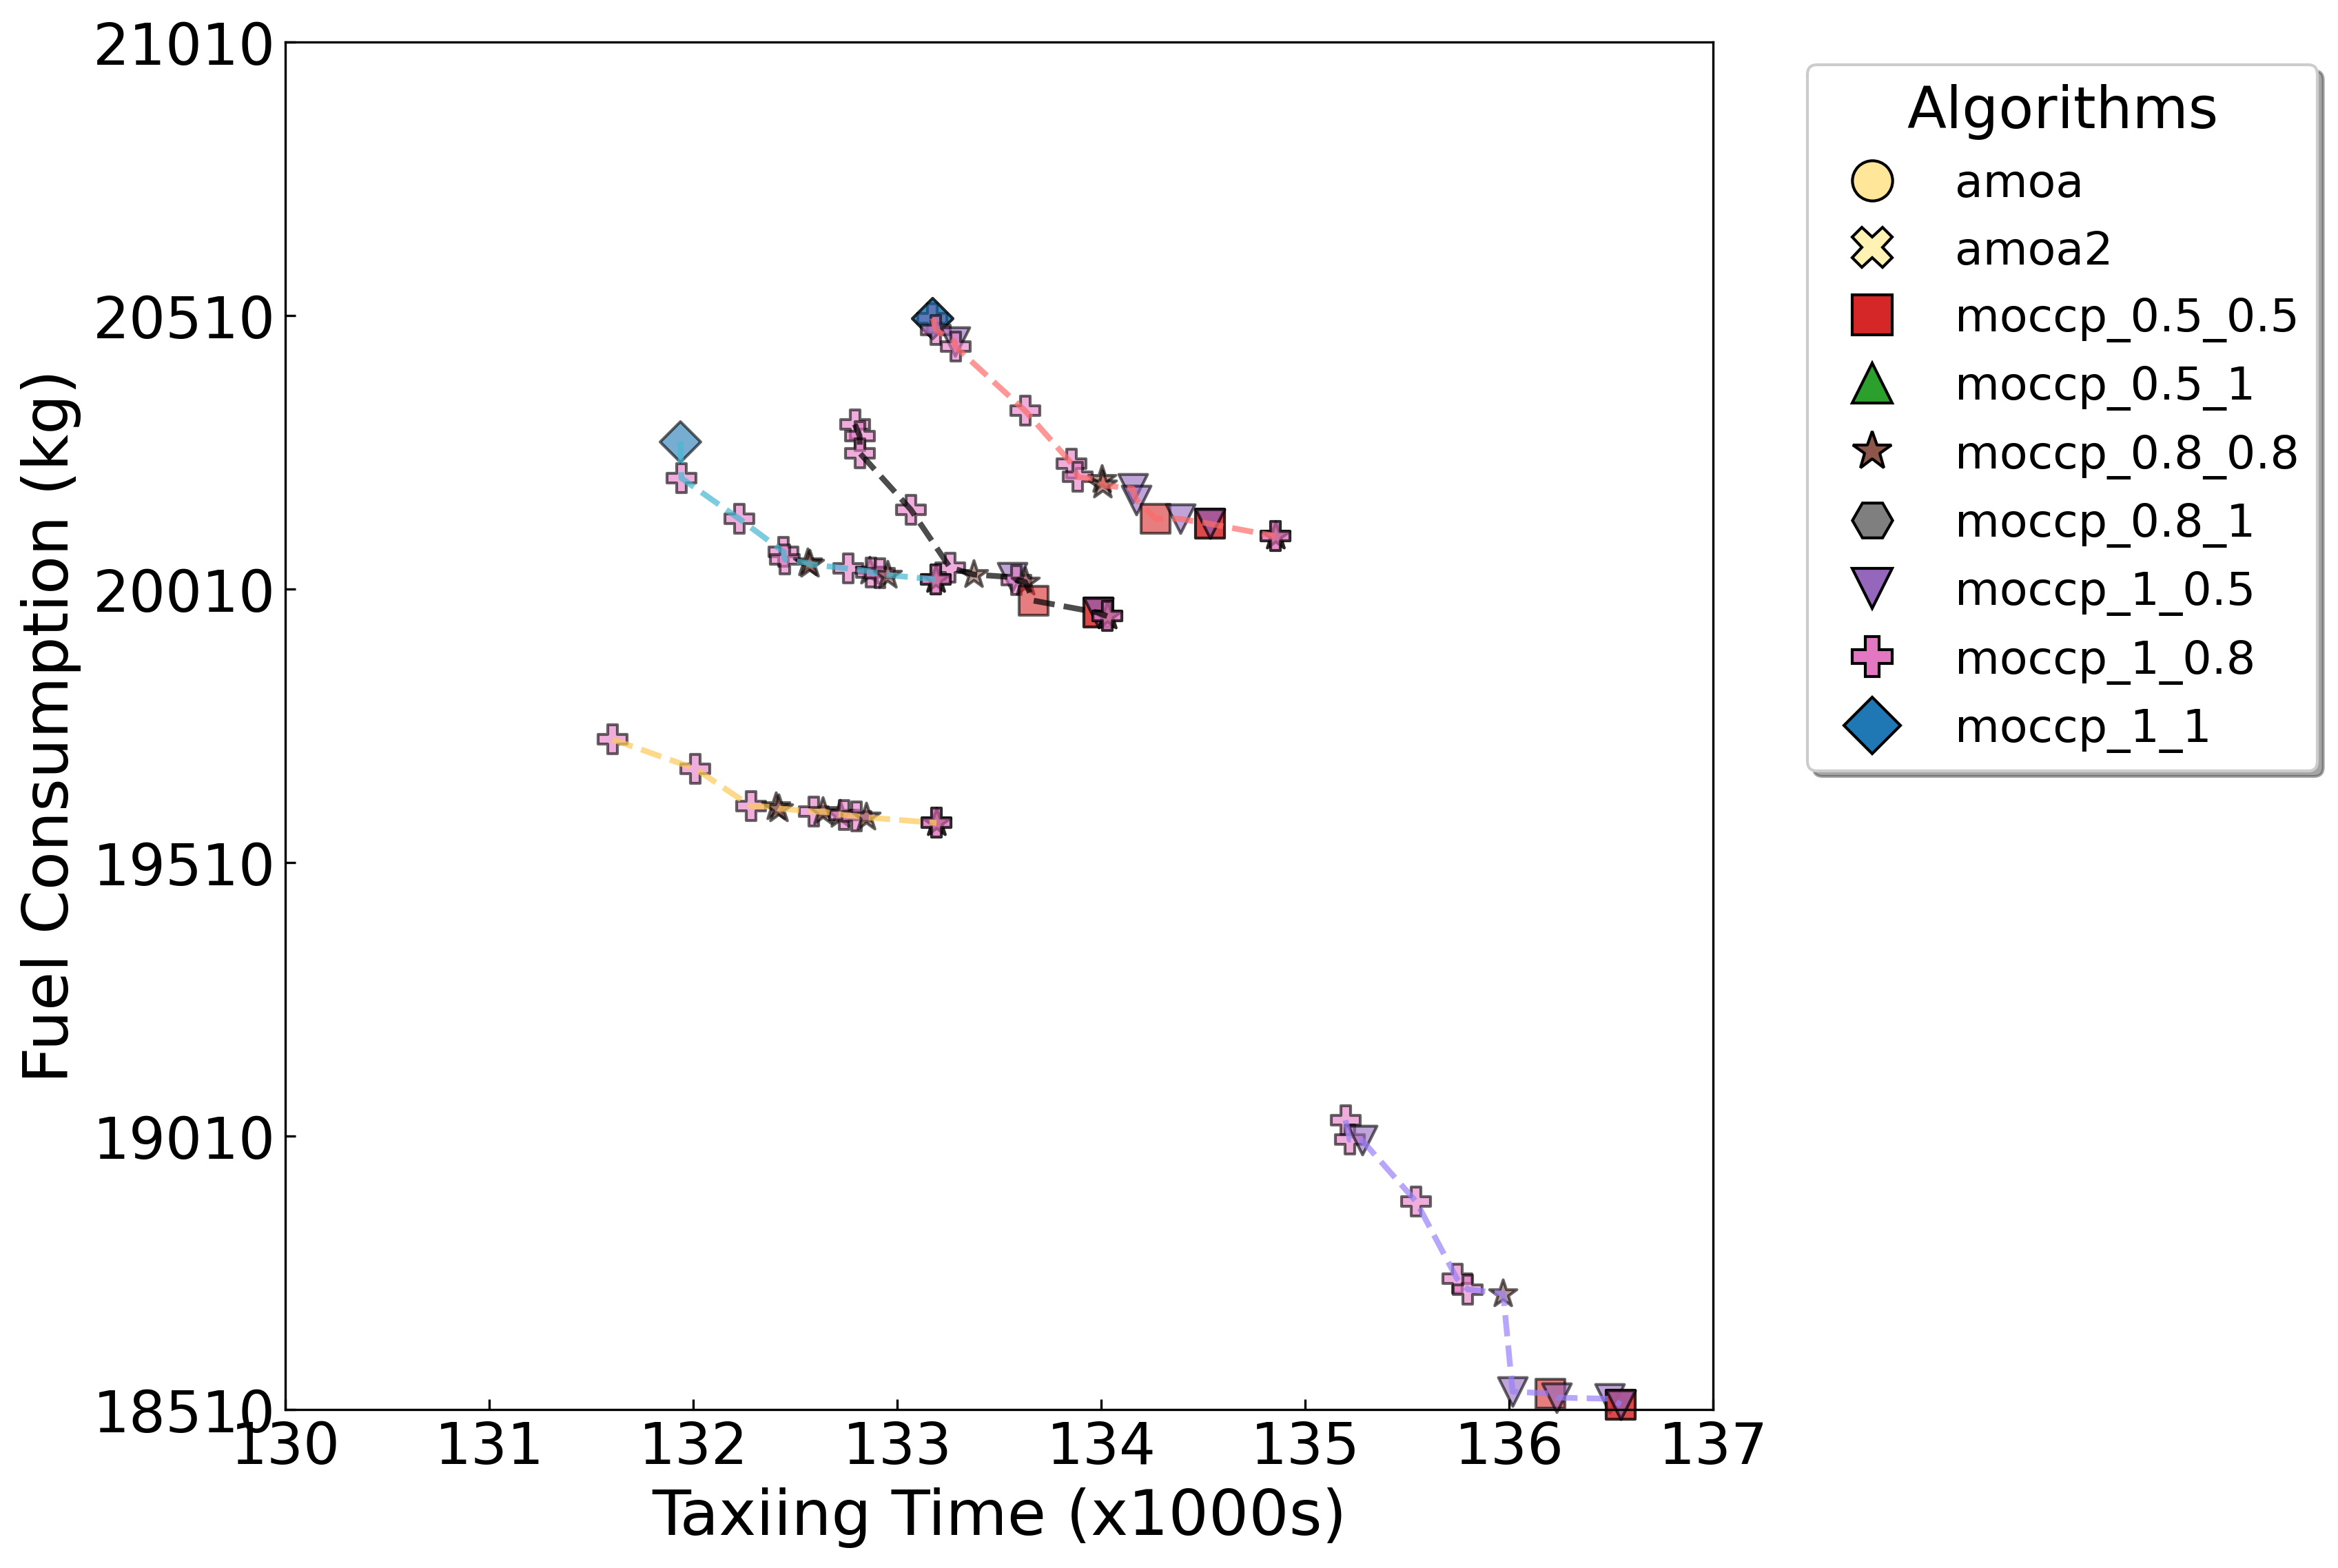
\includegraphics[width=0.44\textwidth]{figures/Traffic_1.0(PF)/0.1/pareto_fronts_colored.png}
    }
    \hspace{0.02\textwidth} 
    \subfloat[Uncertainty level = 0.1\label{fig:un_b}]{
        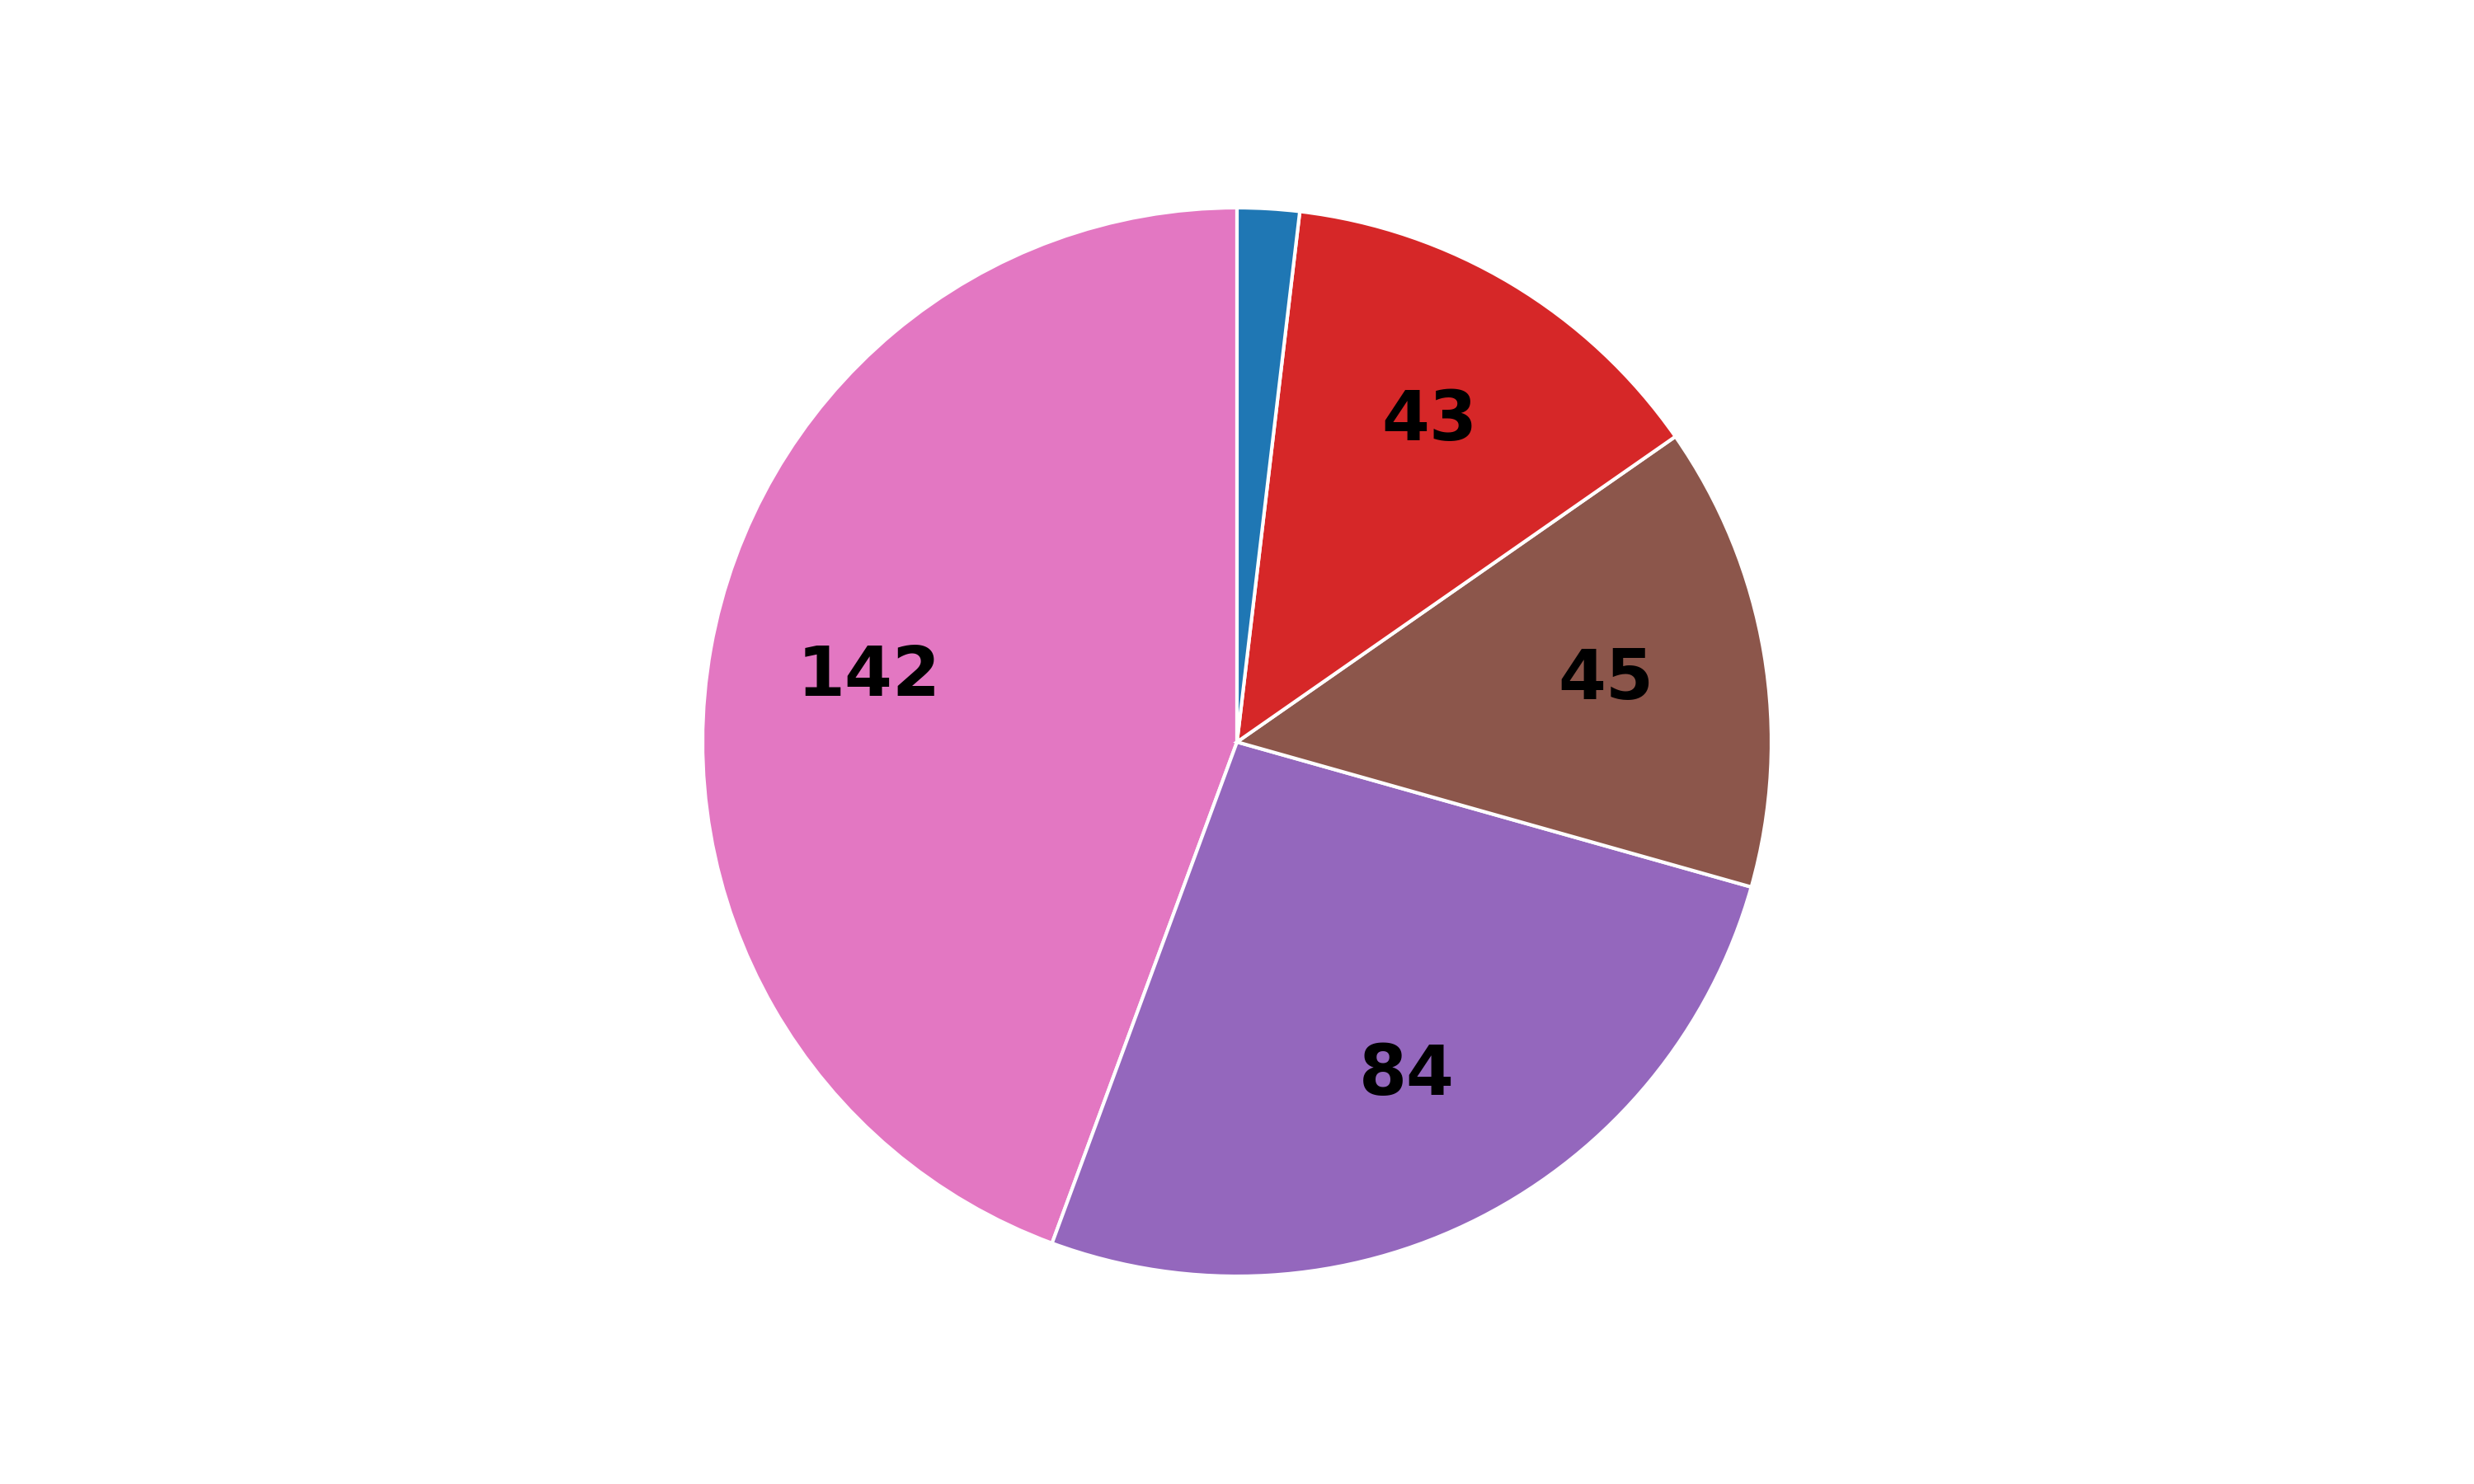
\includegraphics[width=0.44\textwidth]{figures/Traffic_1.0(PF)/0.1/pareto_contribution_piechart.png}
    }
    
    % Row 2: Uncertainty 0.2
    \subfloat[Uncertainty level = 0.2\label{fig:un_c}]{
        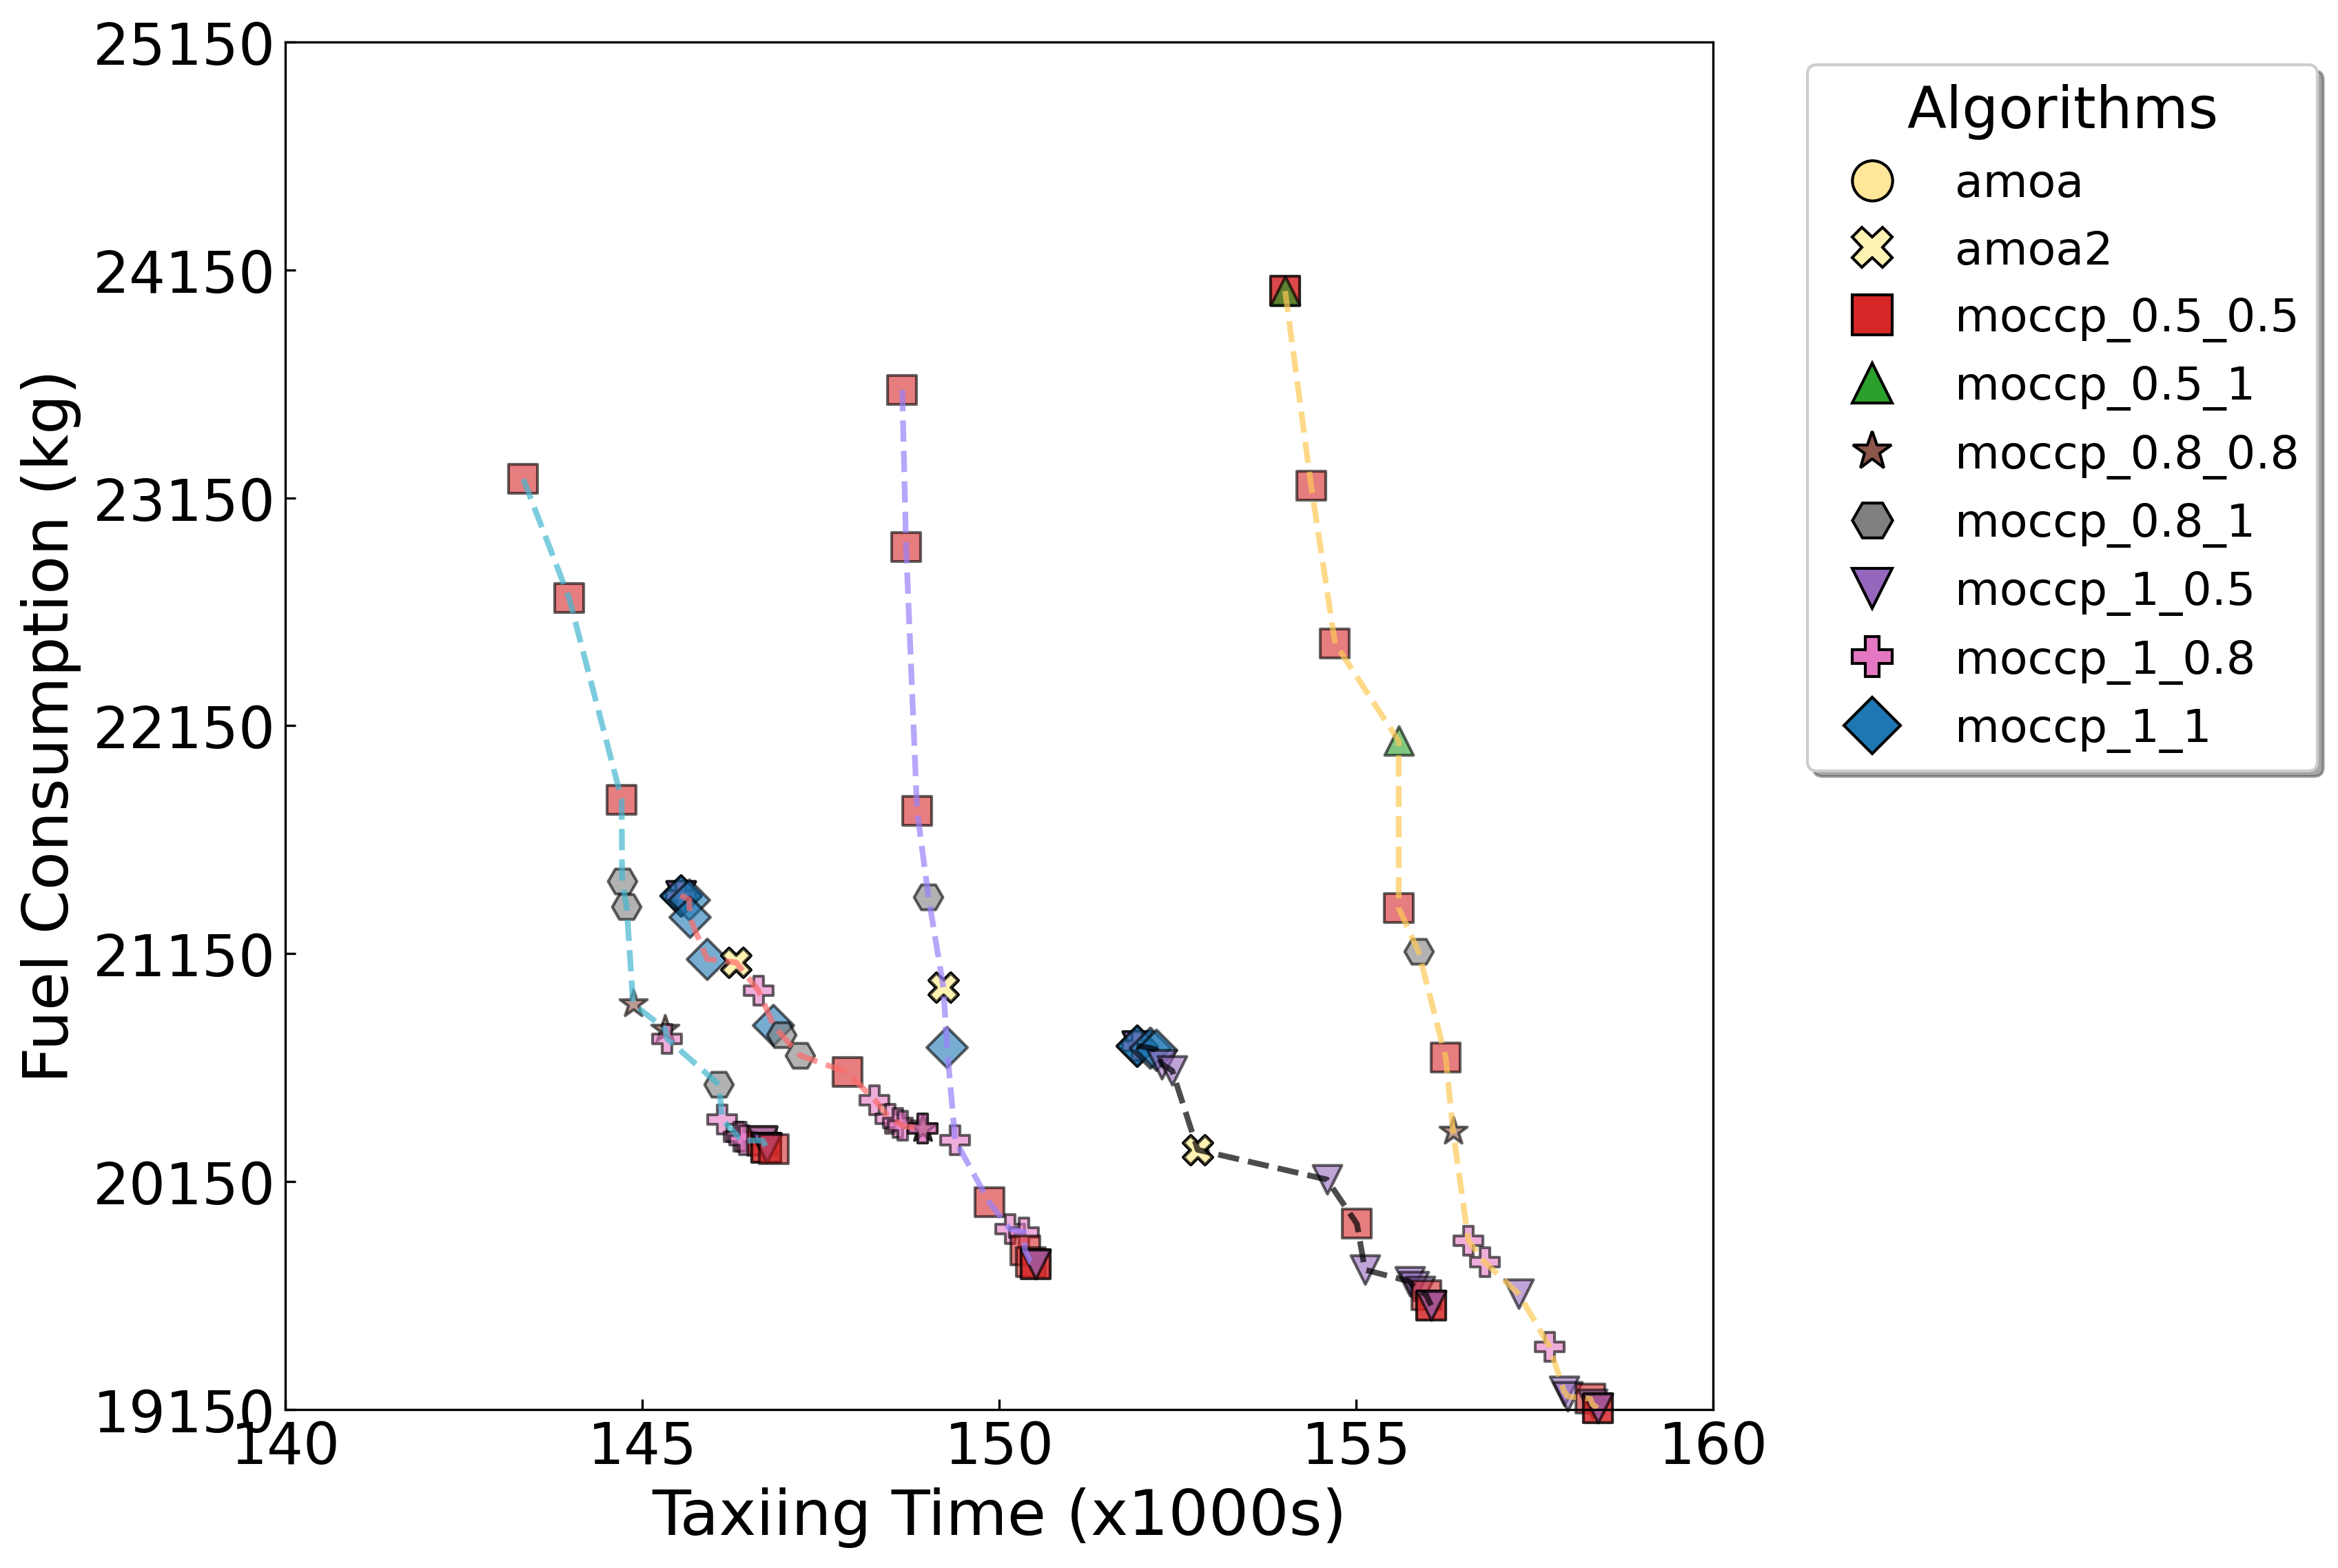
\includegraphics[width=0.44\textwidth]{figures/Traffic_1.0(PF)/0.2/pareto_fronts_colored.png}
    }
    \hspace{0.02\textwidth} 
    \subfloat[Uncertainty level = 0.2\label{fig:un_d}]{
        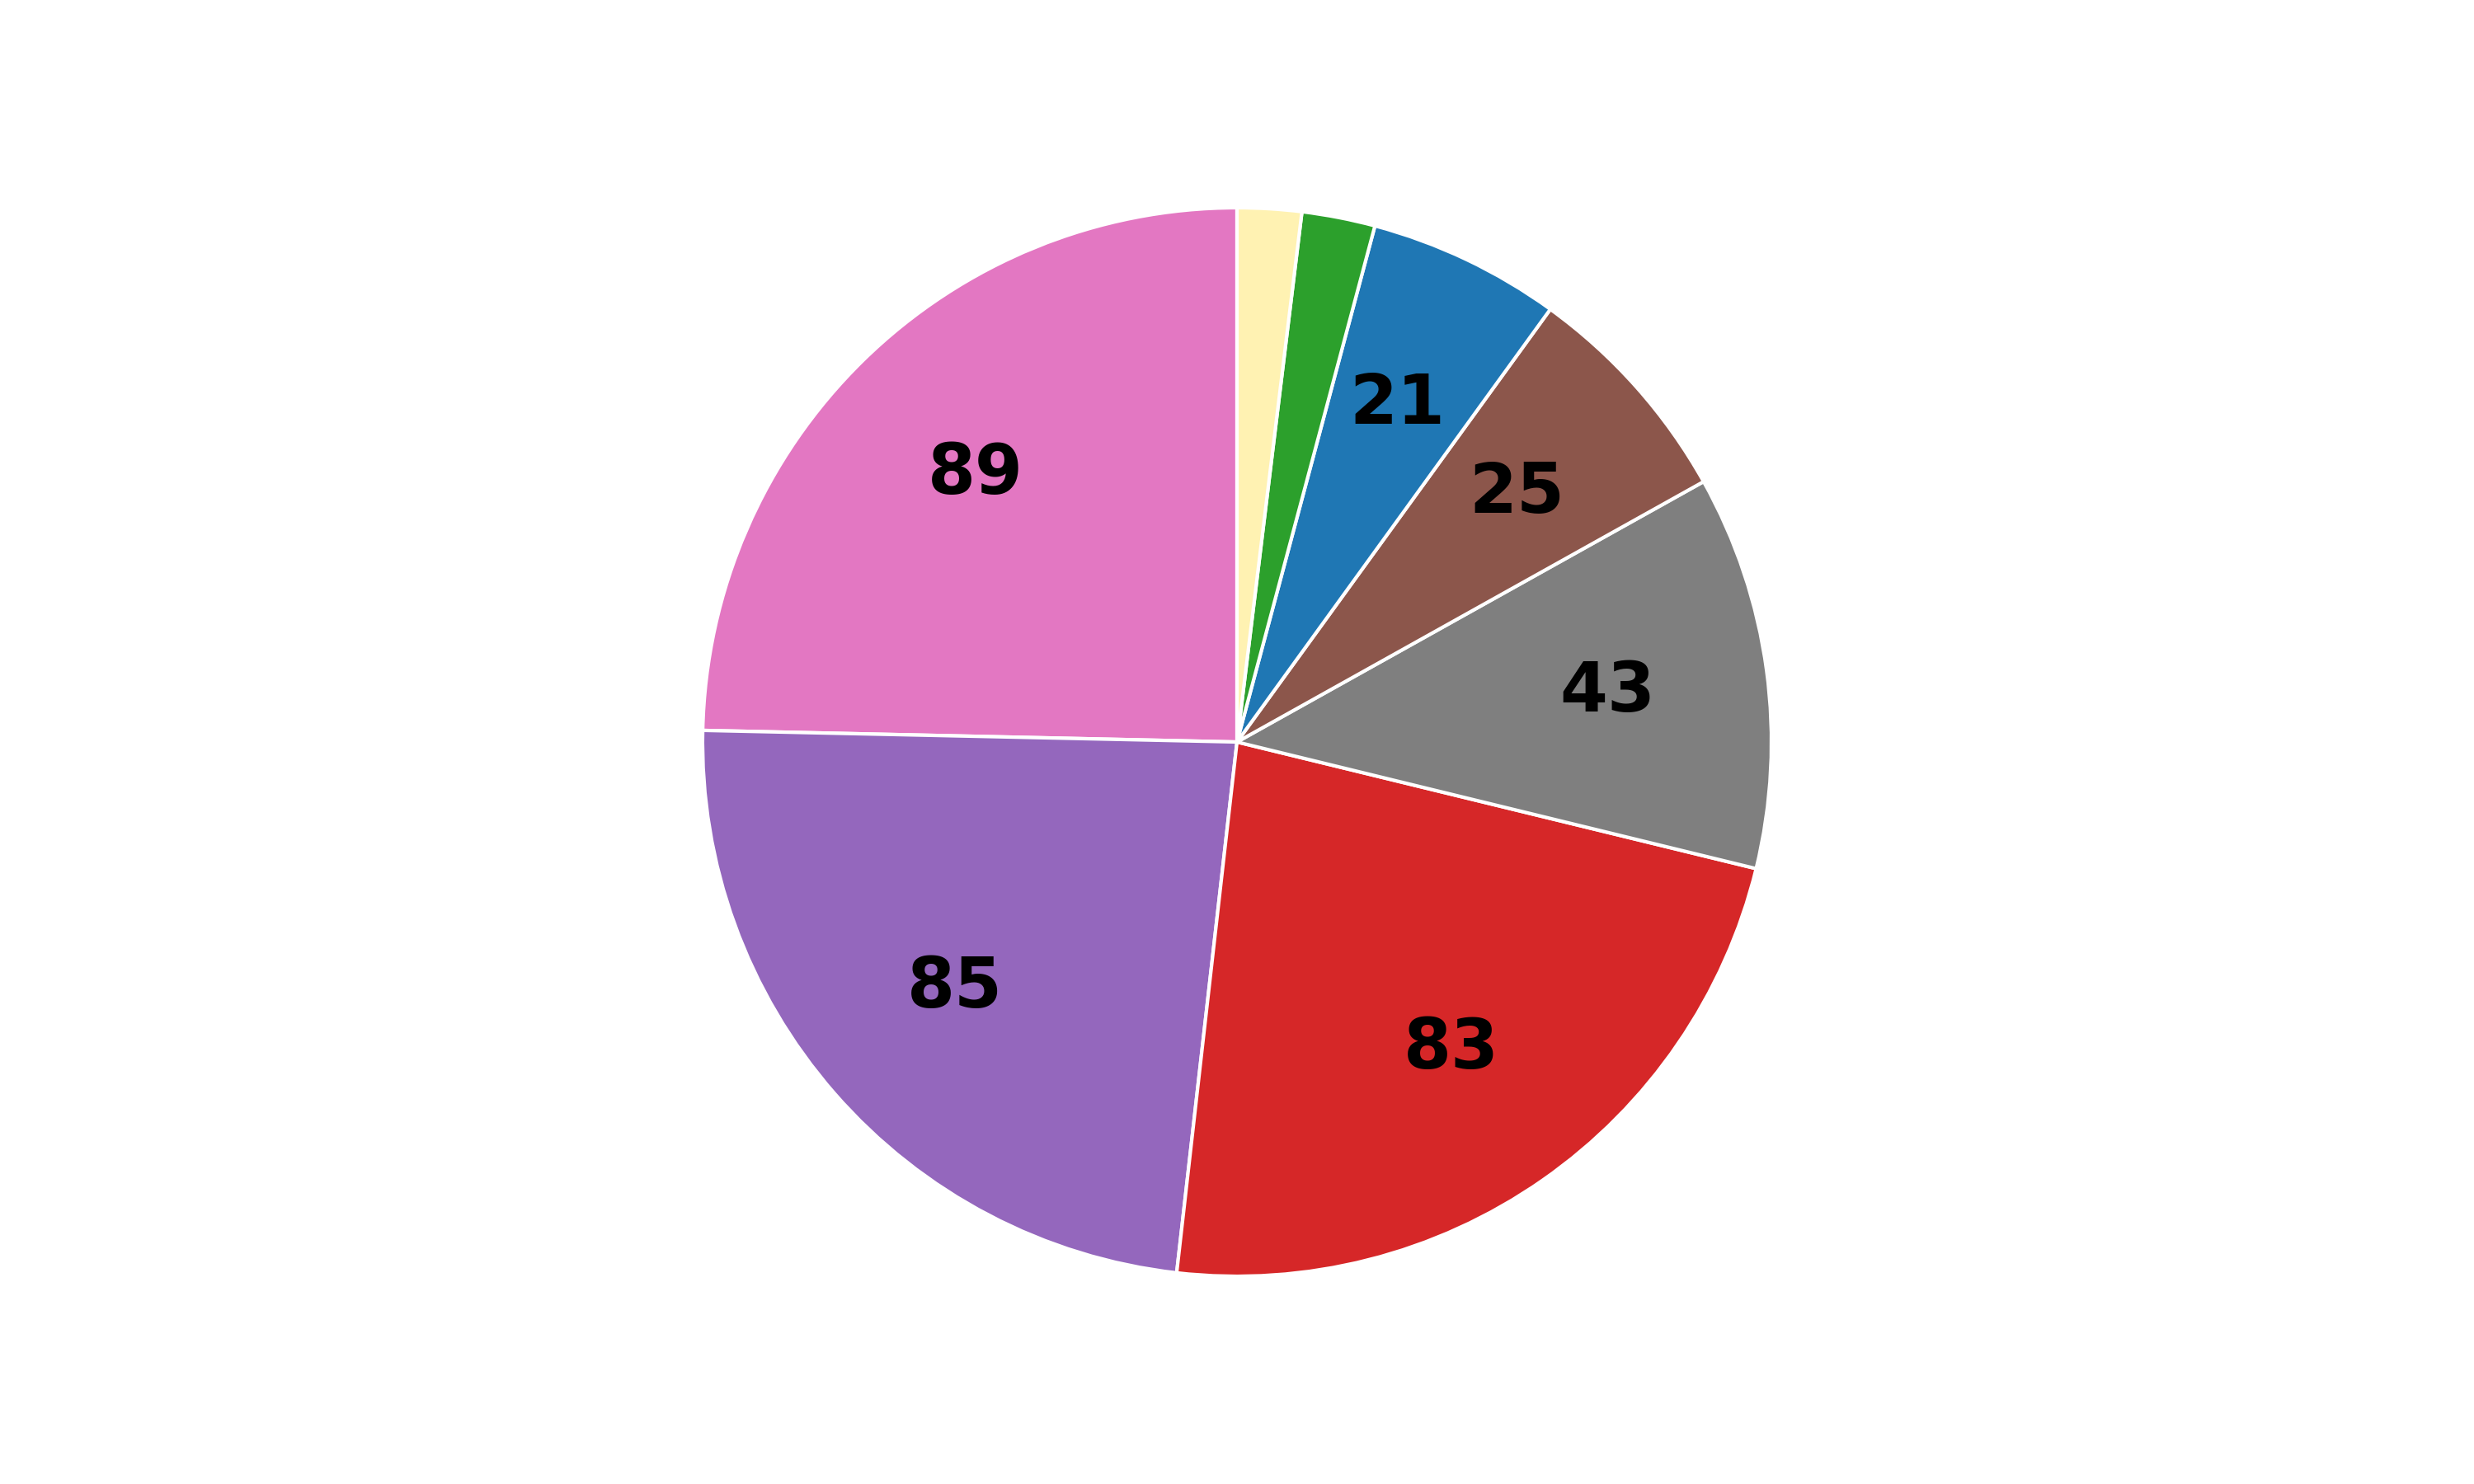
\includegraphics[width=0.44\textwidth]{figures/Traffic_1.0(PF)/0.2/pareto_contribution_piechart.png}
    }
    
    % Row 3: Uncertainty 0.3
    \subfloat[Uncertainty level = 0.3\label{fig:un_e}]{
        \includegraphics[width=0.44\textwidth]{figures/Traffic_1.0(PF)/0.3/pareto_fronts_colored.png}
    }
    \hspace{0.02\textwidth} 
    \subfloat[Uncertainty level = 0.3 \label{fig:un_f}]{
        \includegraphics[width=0.44\textwidth]{figures/Traffic_1.0(PF)/0.3/pareto_contribution_piechart.png}
    }
    
    % Row 4: Uncertainty 0.4
    \subfloat[Uncertainty level = 0.4\label{fig:un_g}]{
        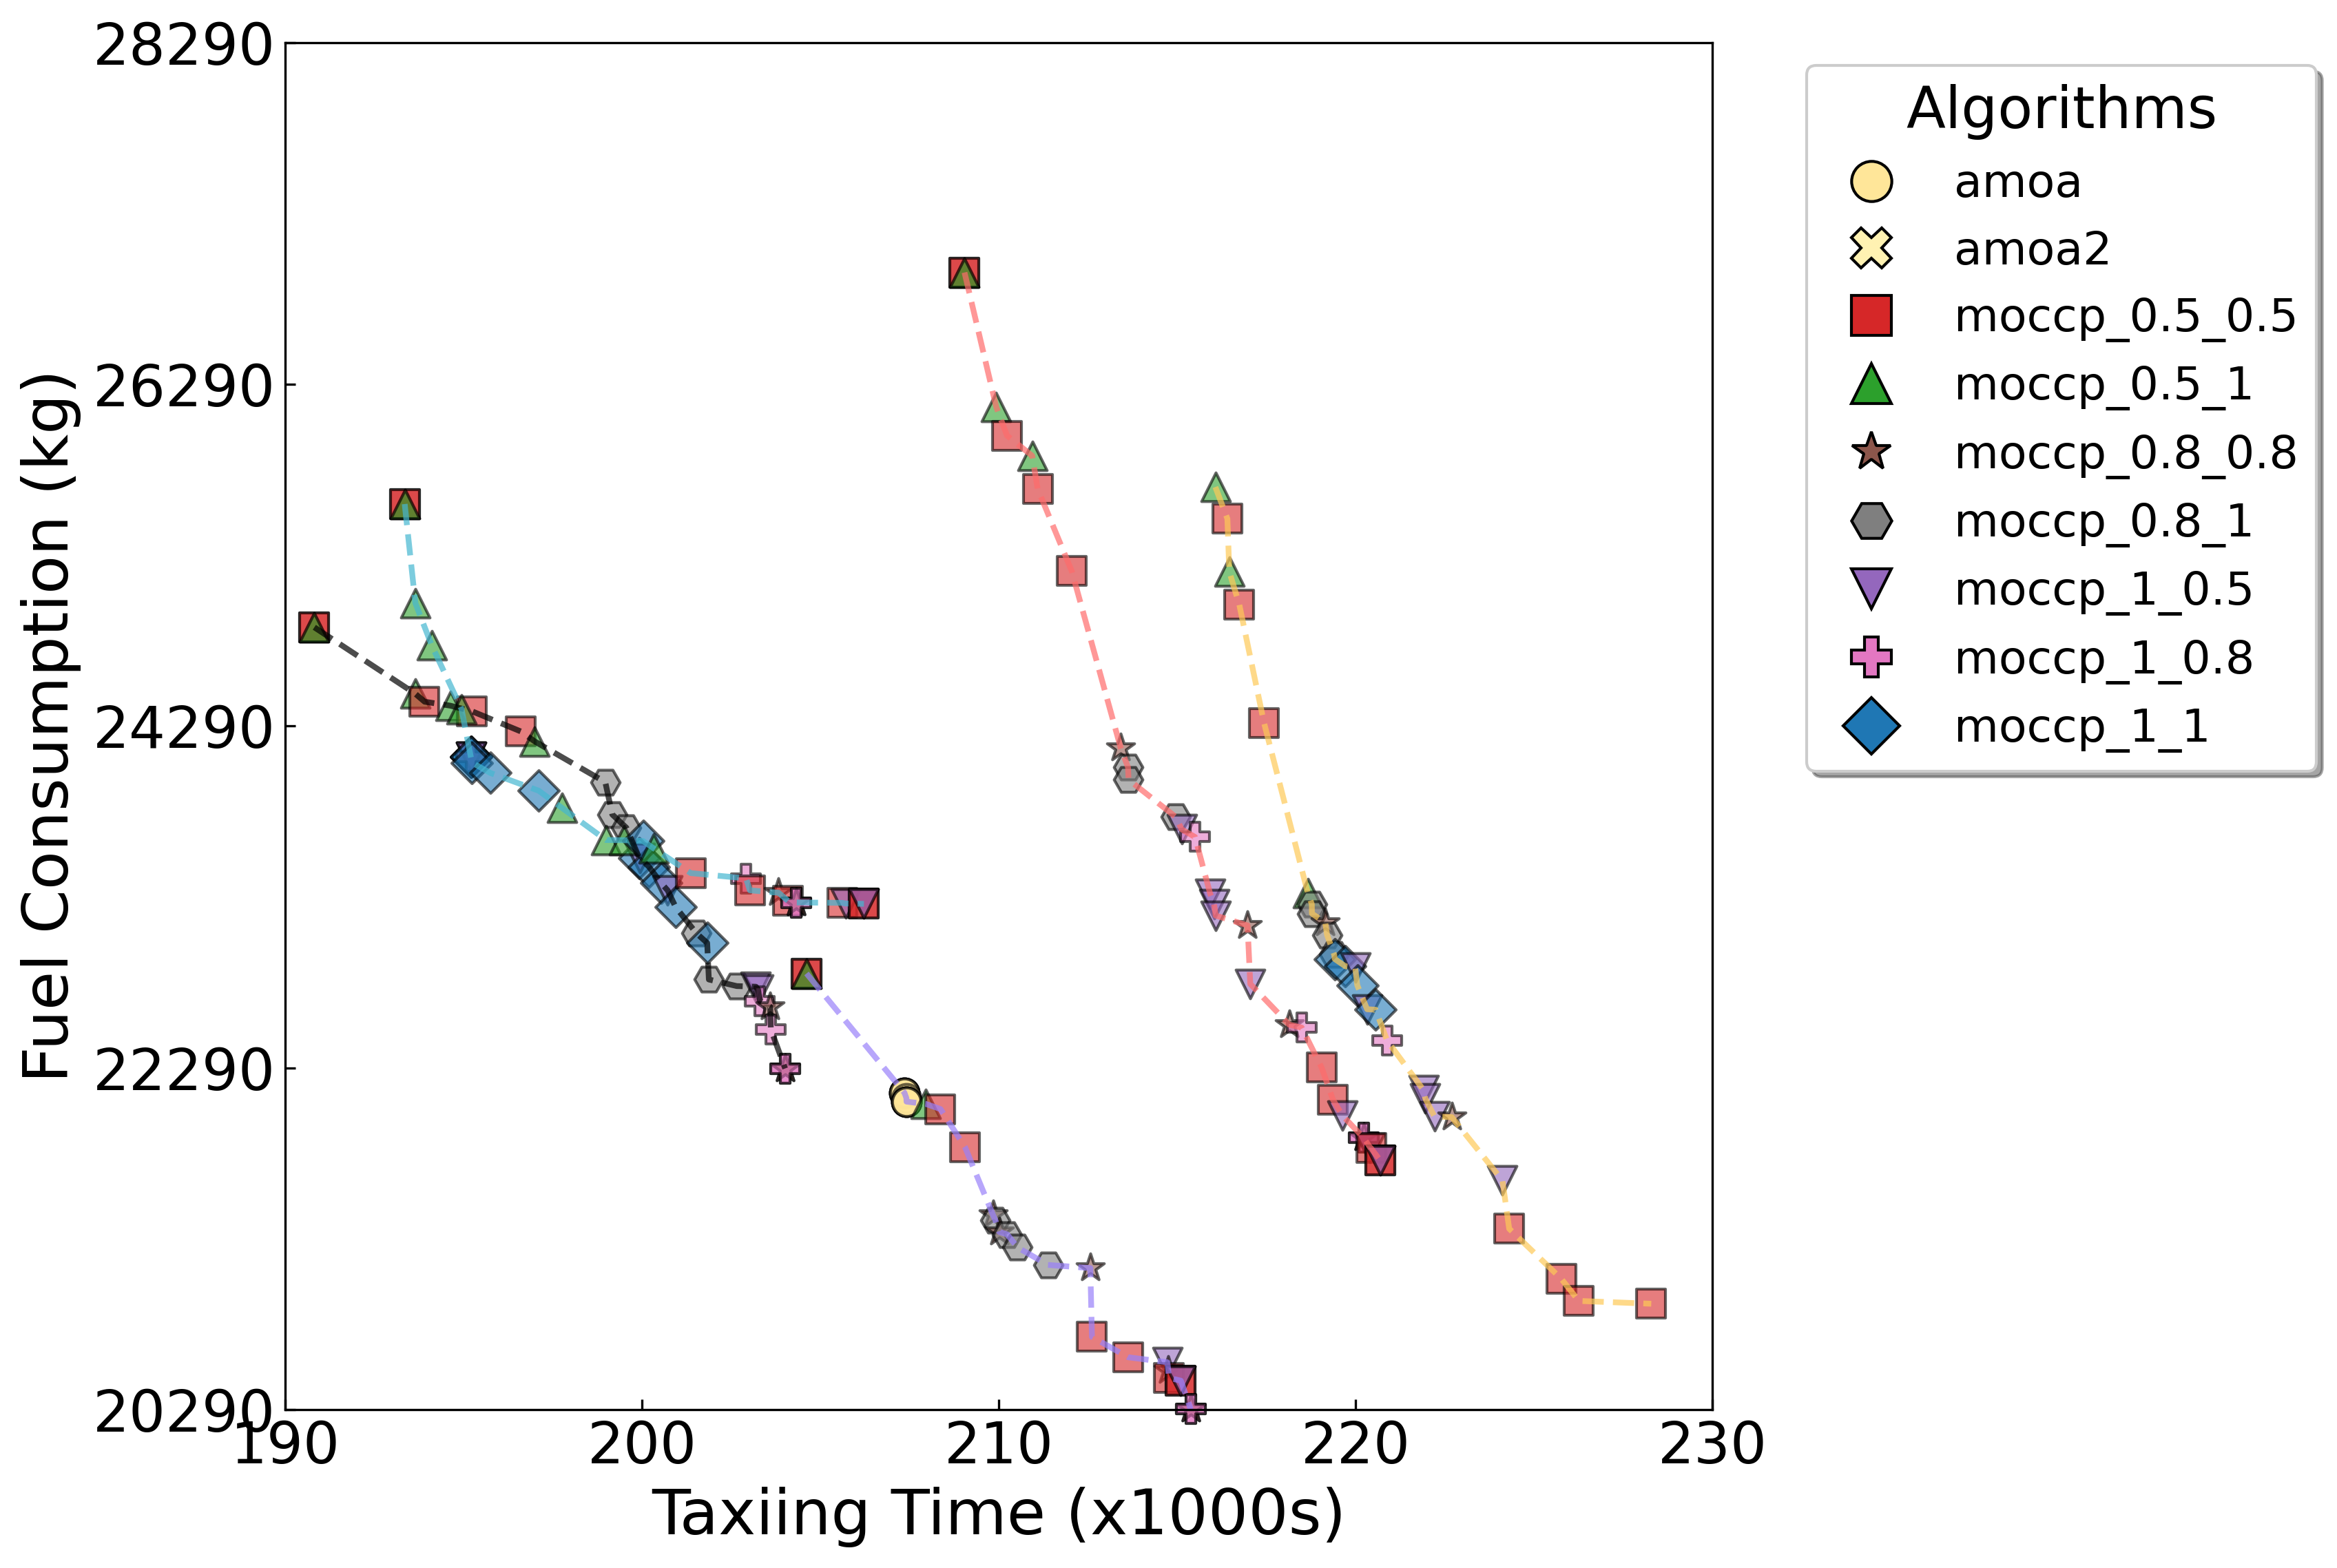
\includegraphics[width=0.44\textwidth]{figures/Traffic_1.0(PF)/0.4/pareto_fronts_colored.png}
    }
    \hspace{0.02\textwidth} 
    \subfloat[Uncertainty level = 0.4\label{fig:un_h}]{
        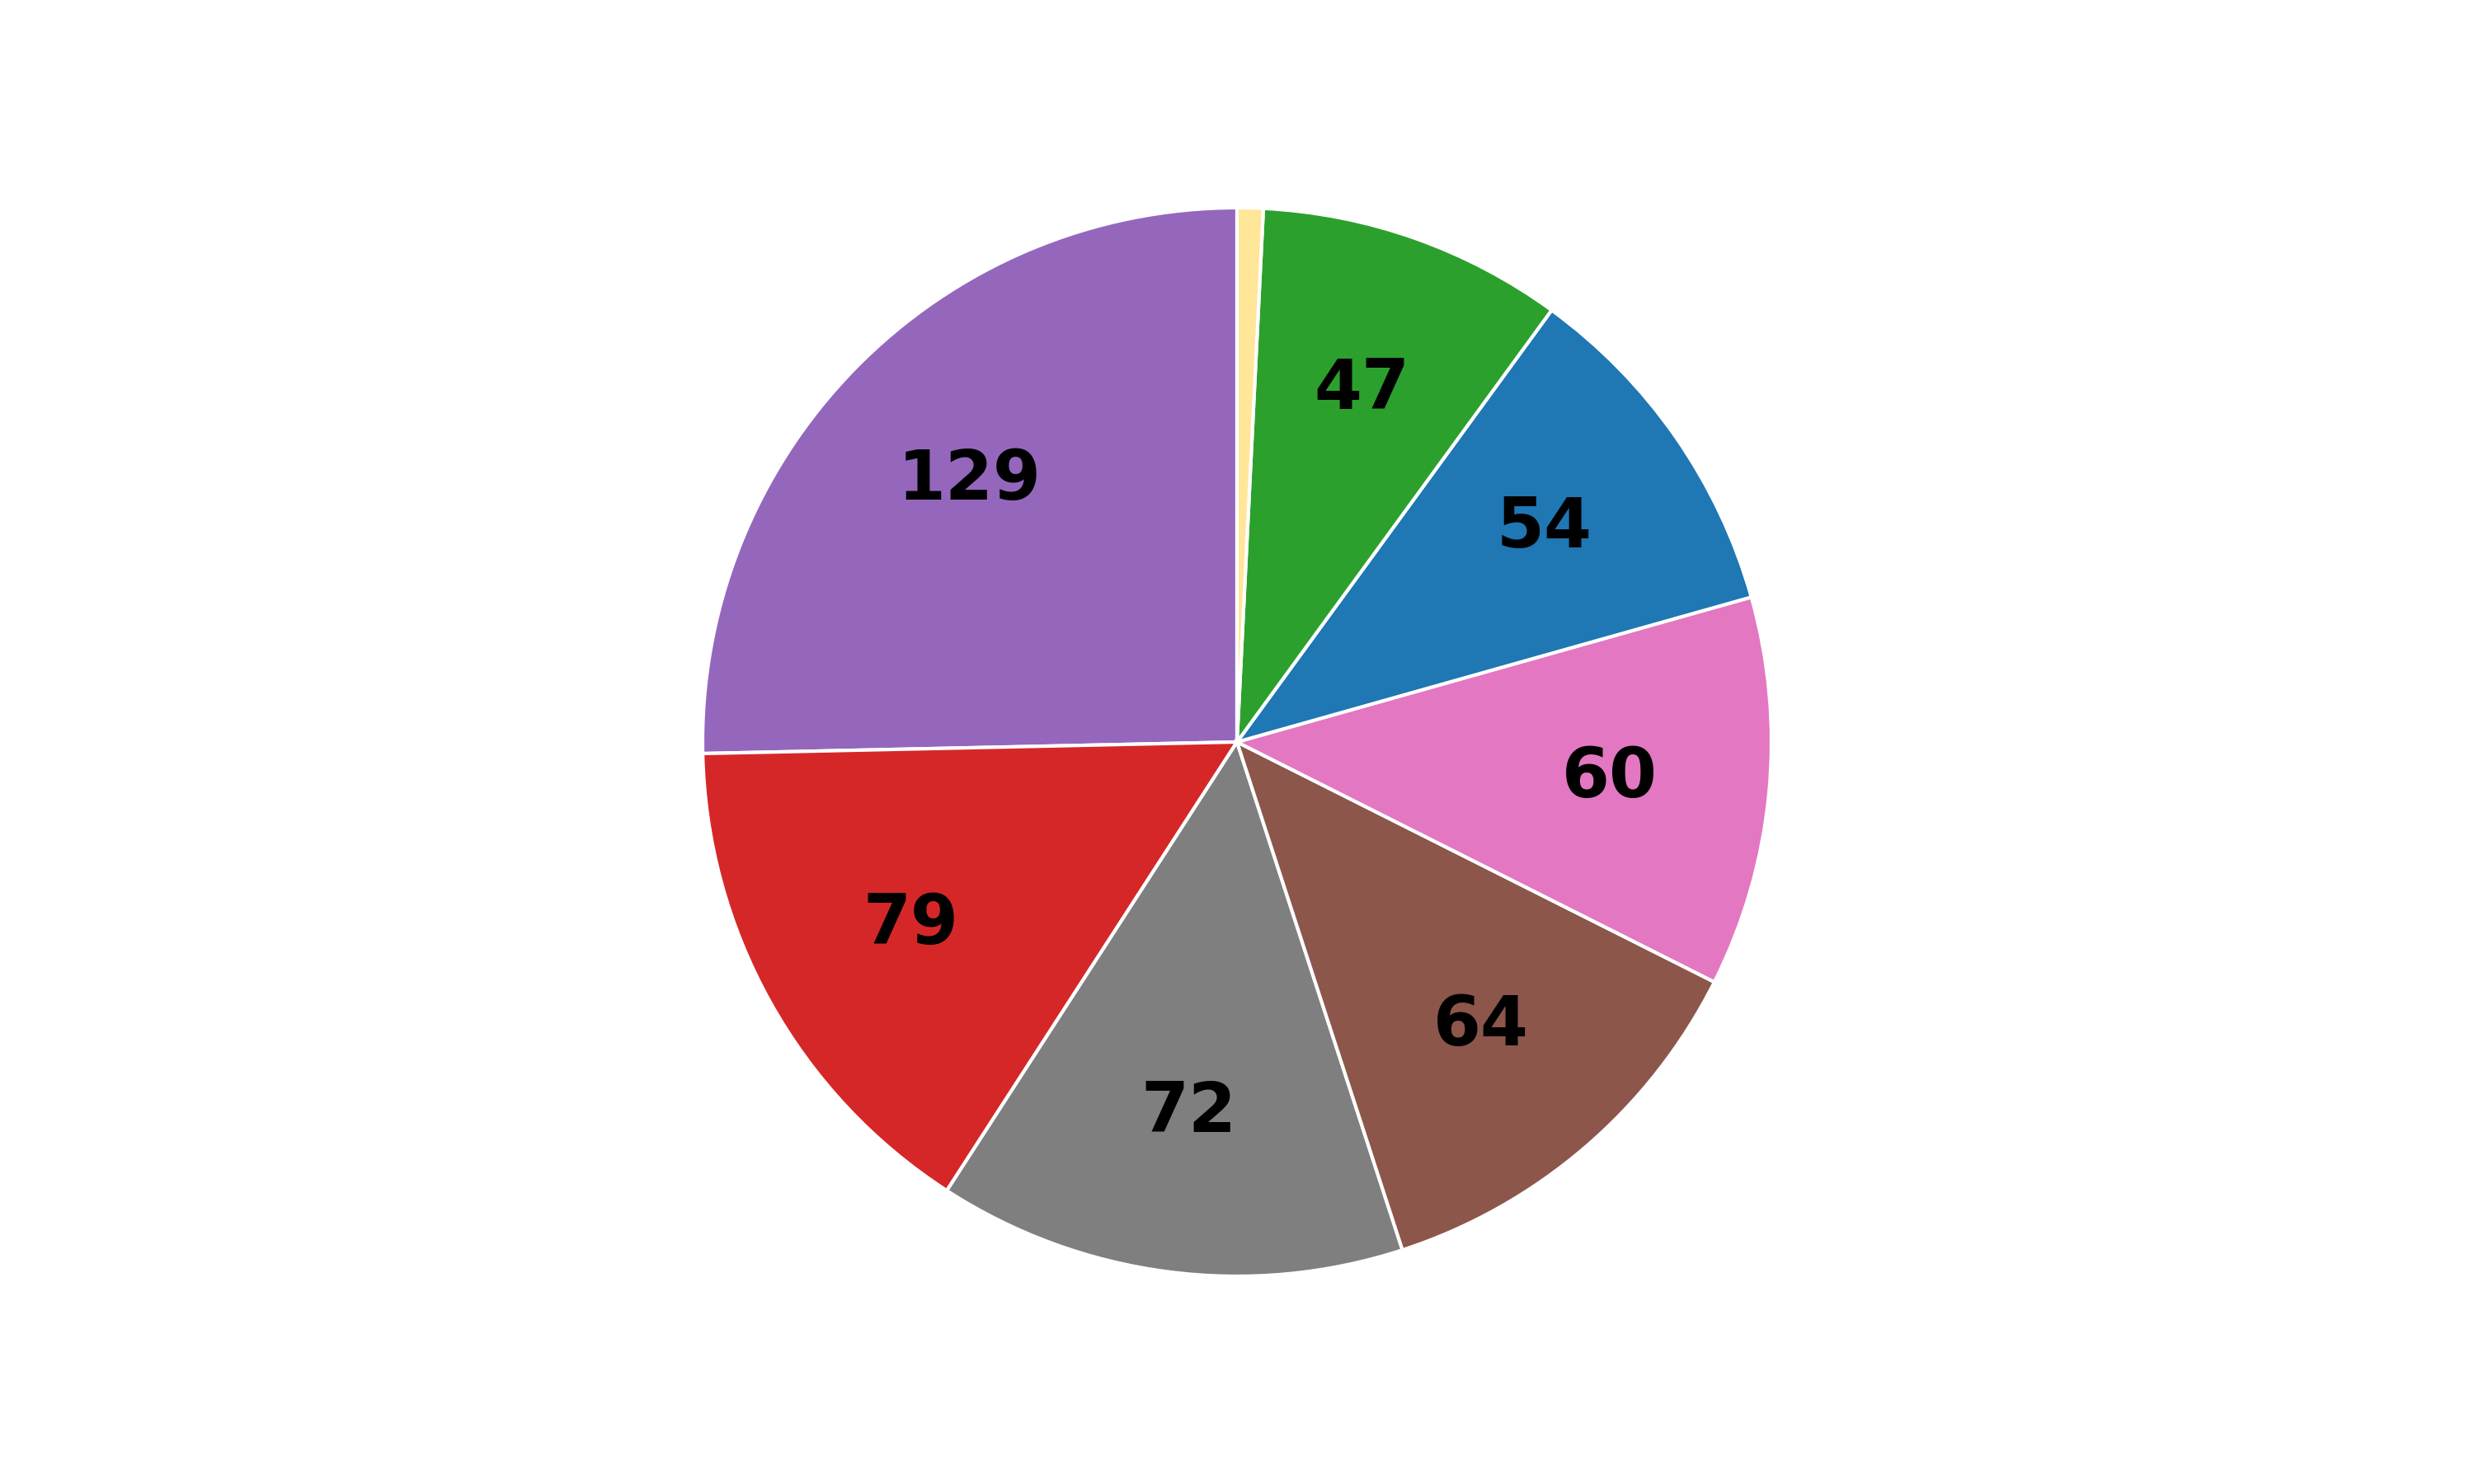
\includegraphics[width=0.44\textwidth]{figures/Traffic_1.0(PF)/0.4/pareto_contribution_piechart.png}
    }
    
    \caption{Comparative analysis of Pareto fronts (5 simulations) and flimsily robust efficient point distributions (30 simulations) under traffic density 1.0 across varying uncertainty levels.}
    \label{fig:un}
\end{figure}

\vspace{0.5em}
\textbf{Performance indicators and comparative evaluation.}
\vspace{0.5em}

To further evaluate algorithm performance, four indicators are introduced. The first is the economic cost, calculated as the weighted sum of the two objectives using unit costs of 0.469 and 0.71, respectively, as suggested in \cite{weiszer2020multi}. The remaining indicators are: taxiing time , fuel consumption, and the total delay time resulting from aircraft conflicts. Delays are measured relative to the unimpeded taxiing time along the allocated routes.

Fig.~\ref{fig:ec} presents the economic cost distributions across varying uncertainty levels (0.1 to 0.4) and five traffic densities ranging from 0.8 to 1.2. As expected, economic costs rise consistently with increasing uncertainty, and this effect is further magnified under higher traffic densities. While the baseline algorithms (\texttt{amoa} and \texttt{amoa2}) initially perform comparably to the CCP-AMOA* algorithms, \texttt{amoa2} slightly outperforms \texttt{amoa} under low-uncertainty and light-traffic scenarios. This may be attributable to their underlying assumptions: \texttt{amoa} allocates routes based on nominal average values, whereas \texttt{amoa2} uses worst-case estimates. Under a low uncertainty level, simulated outcomes align more closely with nominal expectations, favouring the conservative nature of \texttt{amoa2}. However, as the uncertainty level increases, deviations from the nominal scenario become more likely, leading to degraded performance of both, especially \texttt{amoa2}, which suffers from both higher costs and greater cost variability. In contrast, the CCP-AMOA* algorithms demonstrate superior robustness and cost efficiency under heightened uncertainties. In particular, algorithms such as \texttt{moccp\_1\_0.5}, \texttt{moccp\_0.8\_0.8}, and \texttt{moccp\_1\_0.8} consistently demonstrate lower median costs and narrower interquartile ranges, reflecting their enhanced stability. These observations align with the trends previously identified in the Pareto front analysis. The growing interquartile ranges and prevalence of outliers under high uncertainty levels highlight growing cost variability, especially in dense traffic scenarios. Notably, CCP-AMOA* algorithms that emphasise more conservative confidence levels in taxiing time consistently produce more robust economic outcomes. This can be attributed to the significant contribution of taxiing time to the overall economic cost, as well as its cascading effect on fuel consumption, where increased taxiing delays lead to higher fuel consumption due to conflicts and idling.

\begin{figure}[htp]
    \centering
    
    % Row 1
    \subfloat[Traffic density = 0.8\label{fig:ec_a}]{
        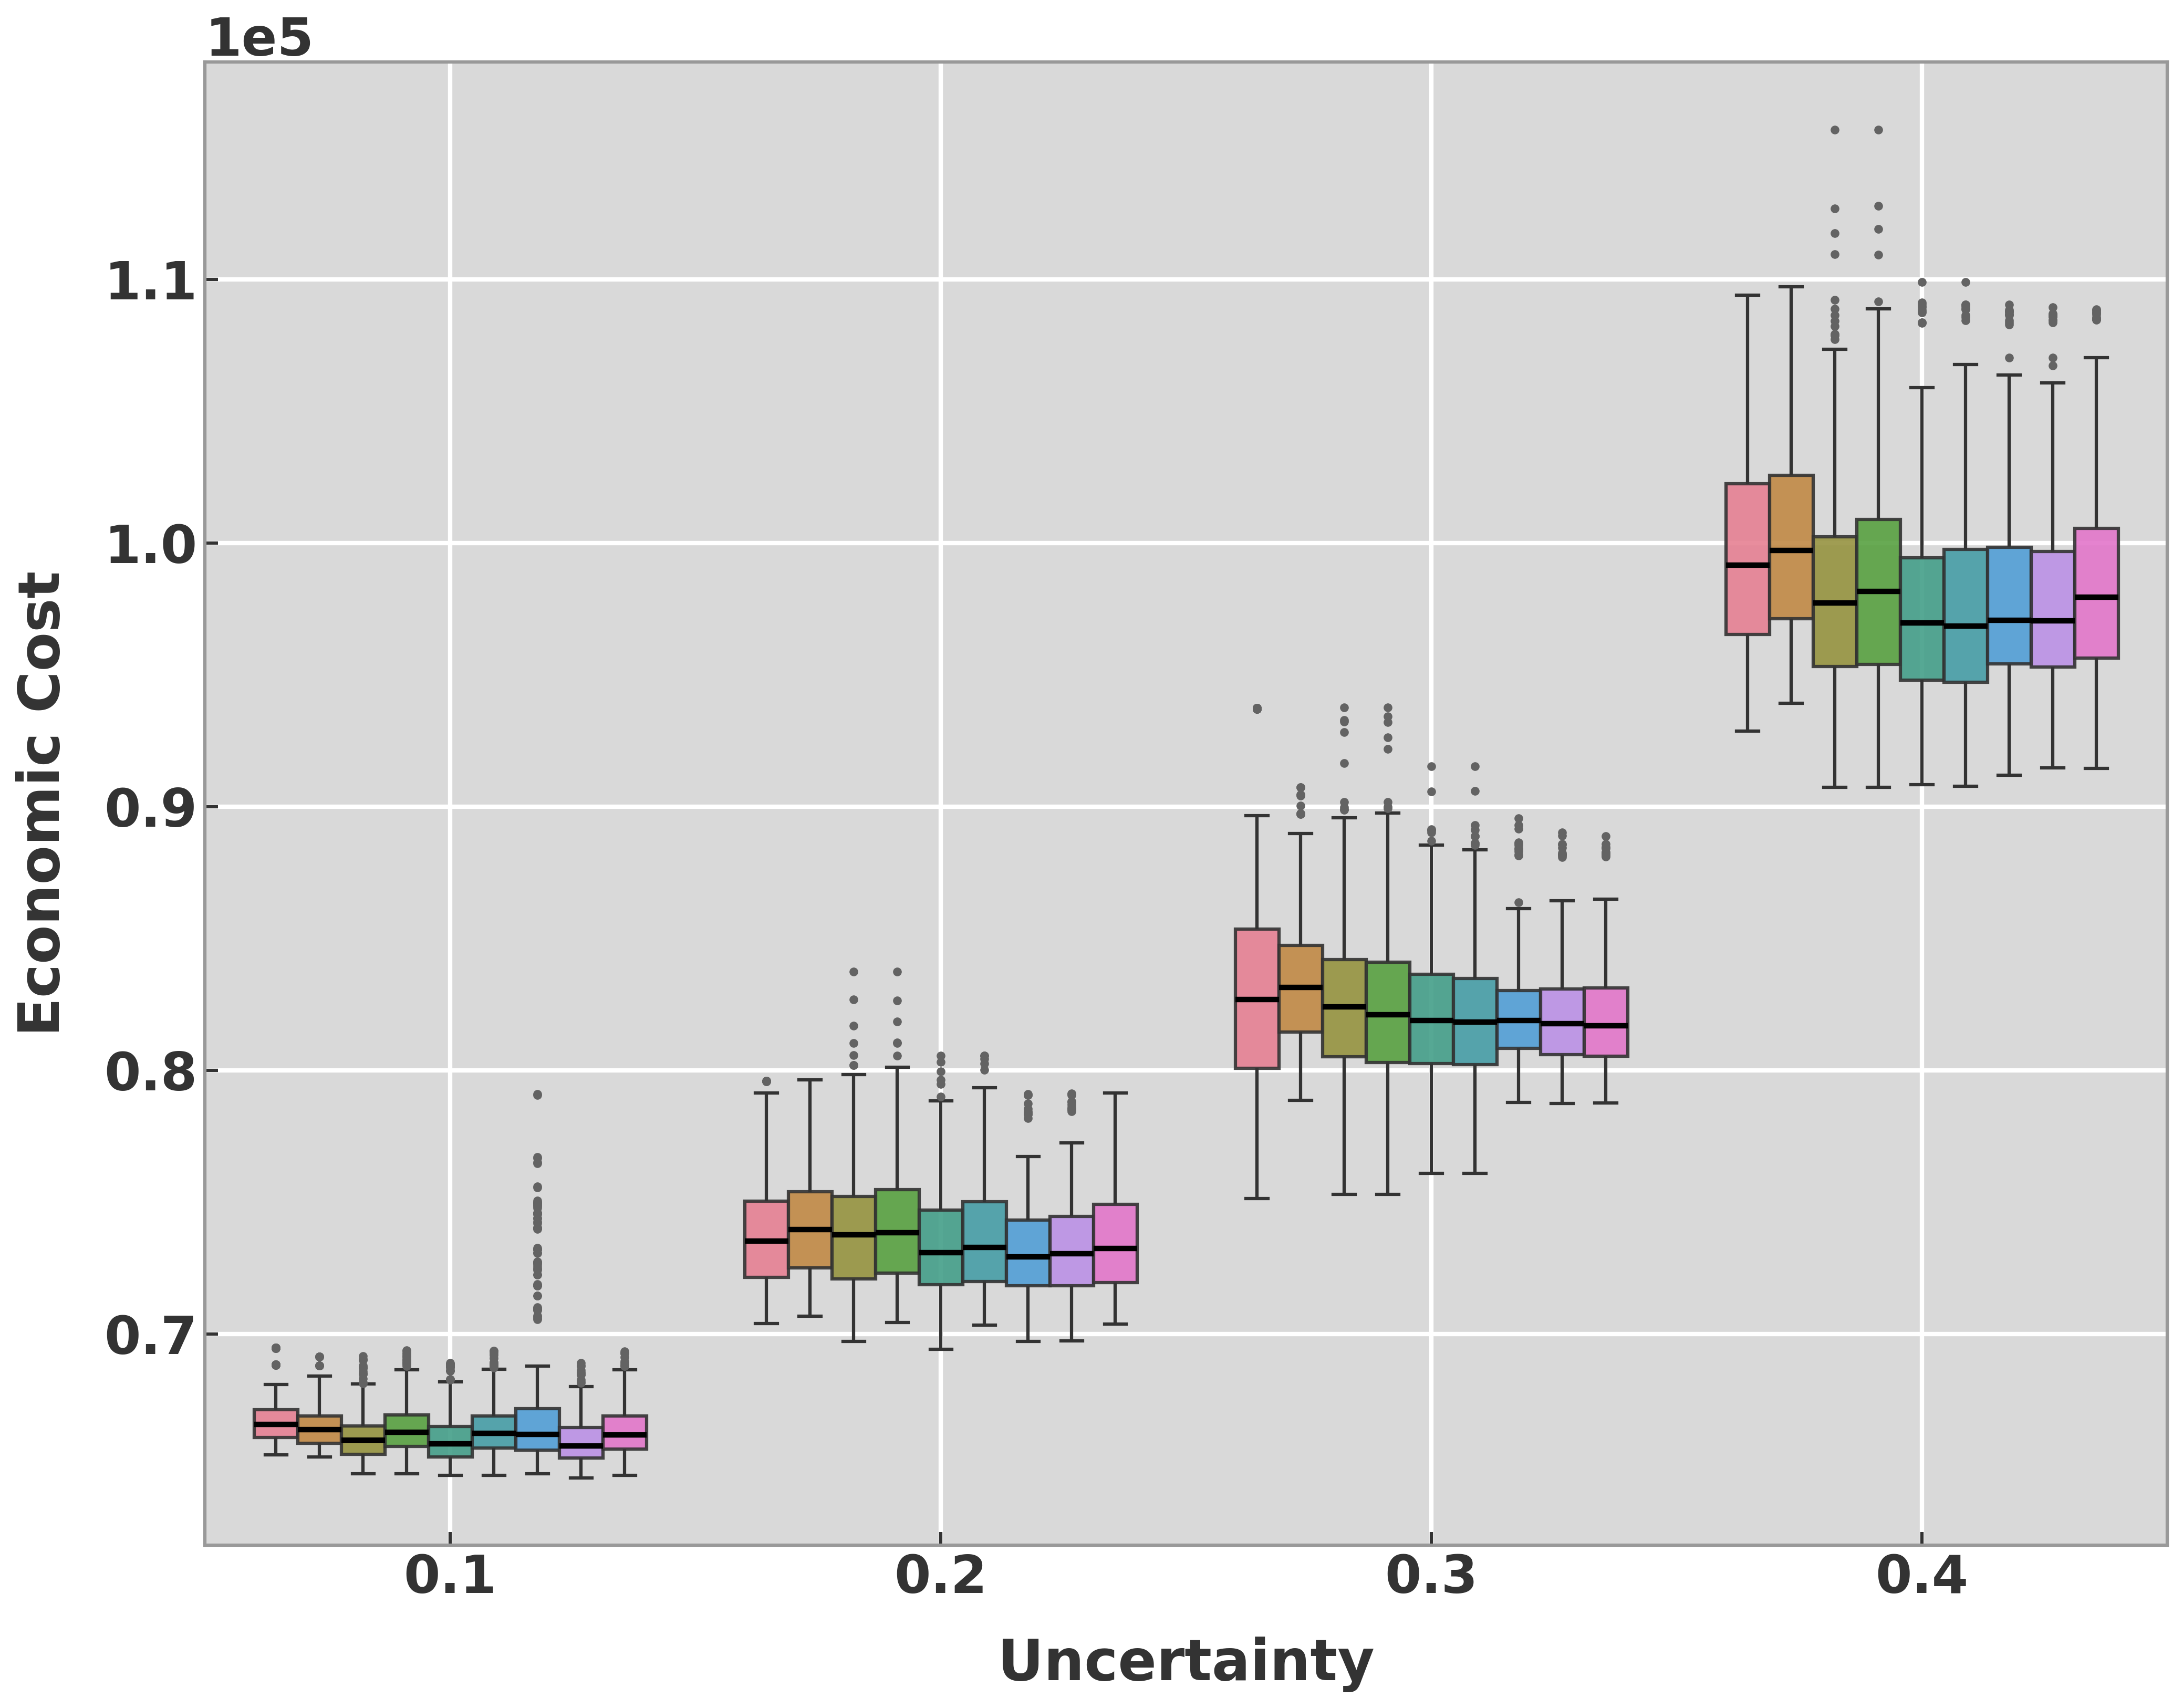
\includegraphics[width=0.45\textwidth]{figures/Traffic_0.8/traffic_0.8_economic_cost.png}
    }
    \hfill
    \subfloat[Traffic density = 0.9\label{fig:ec_b}]{
        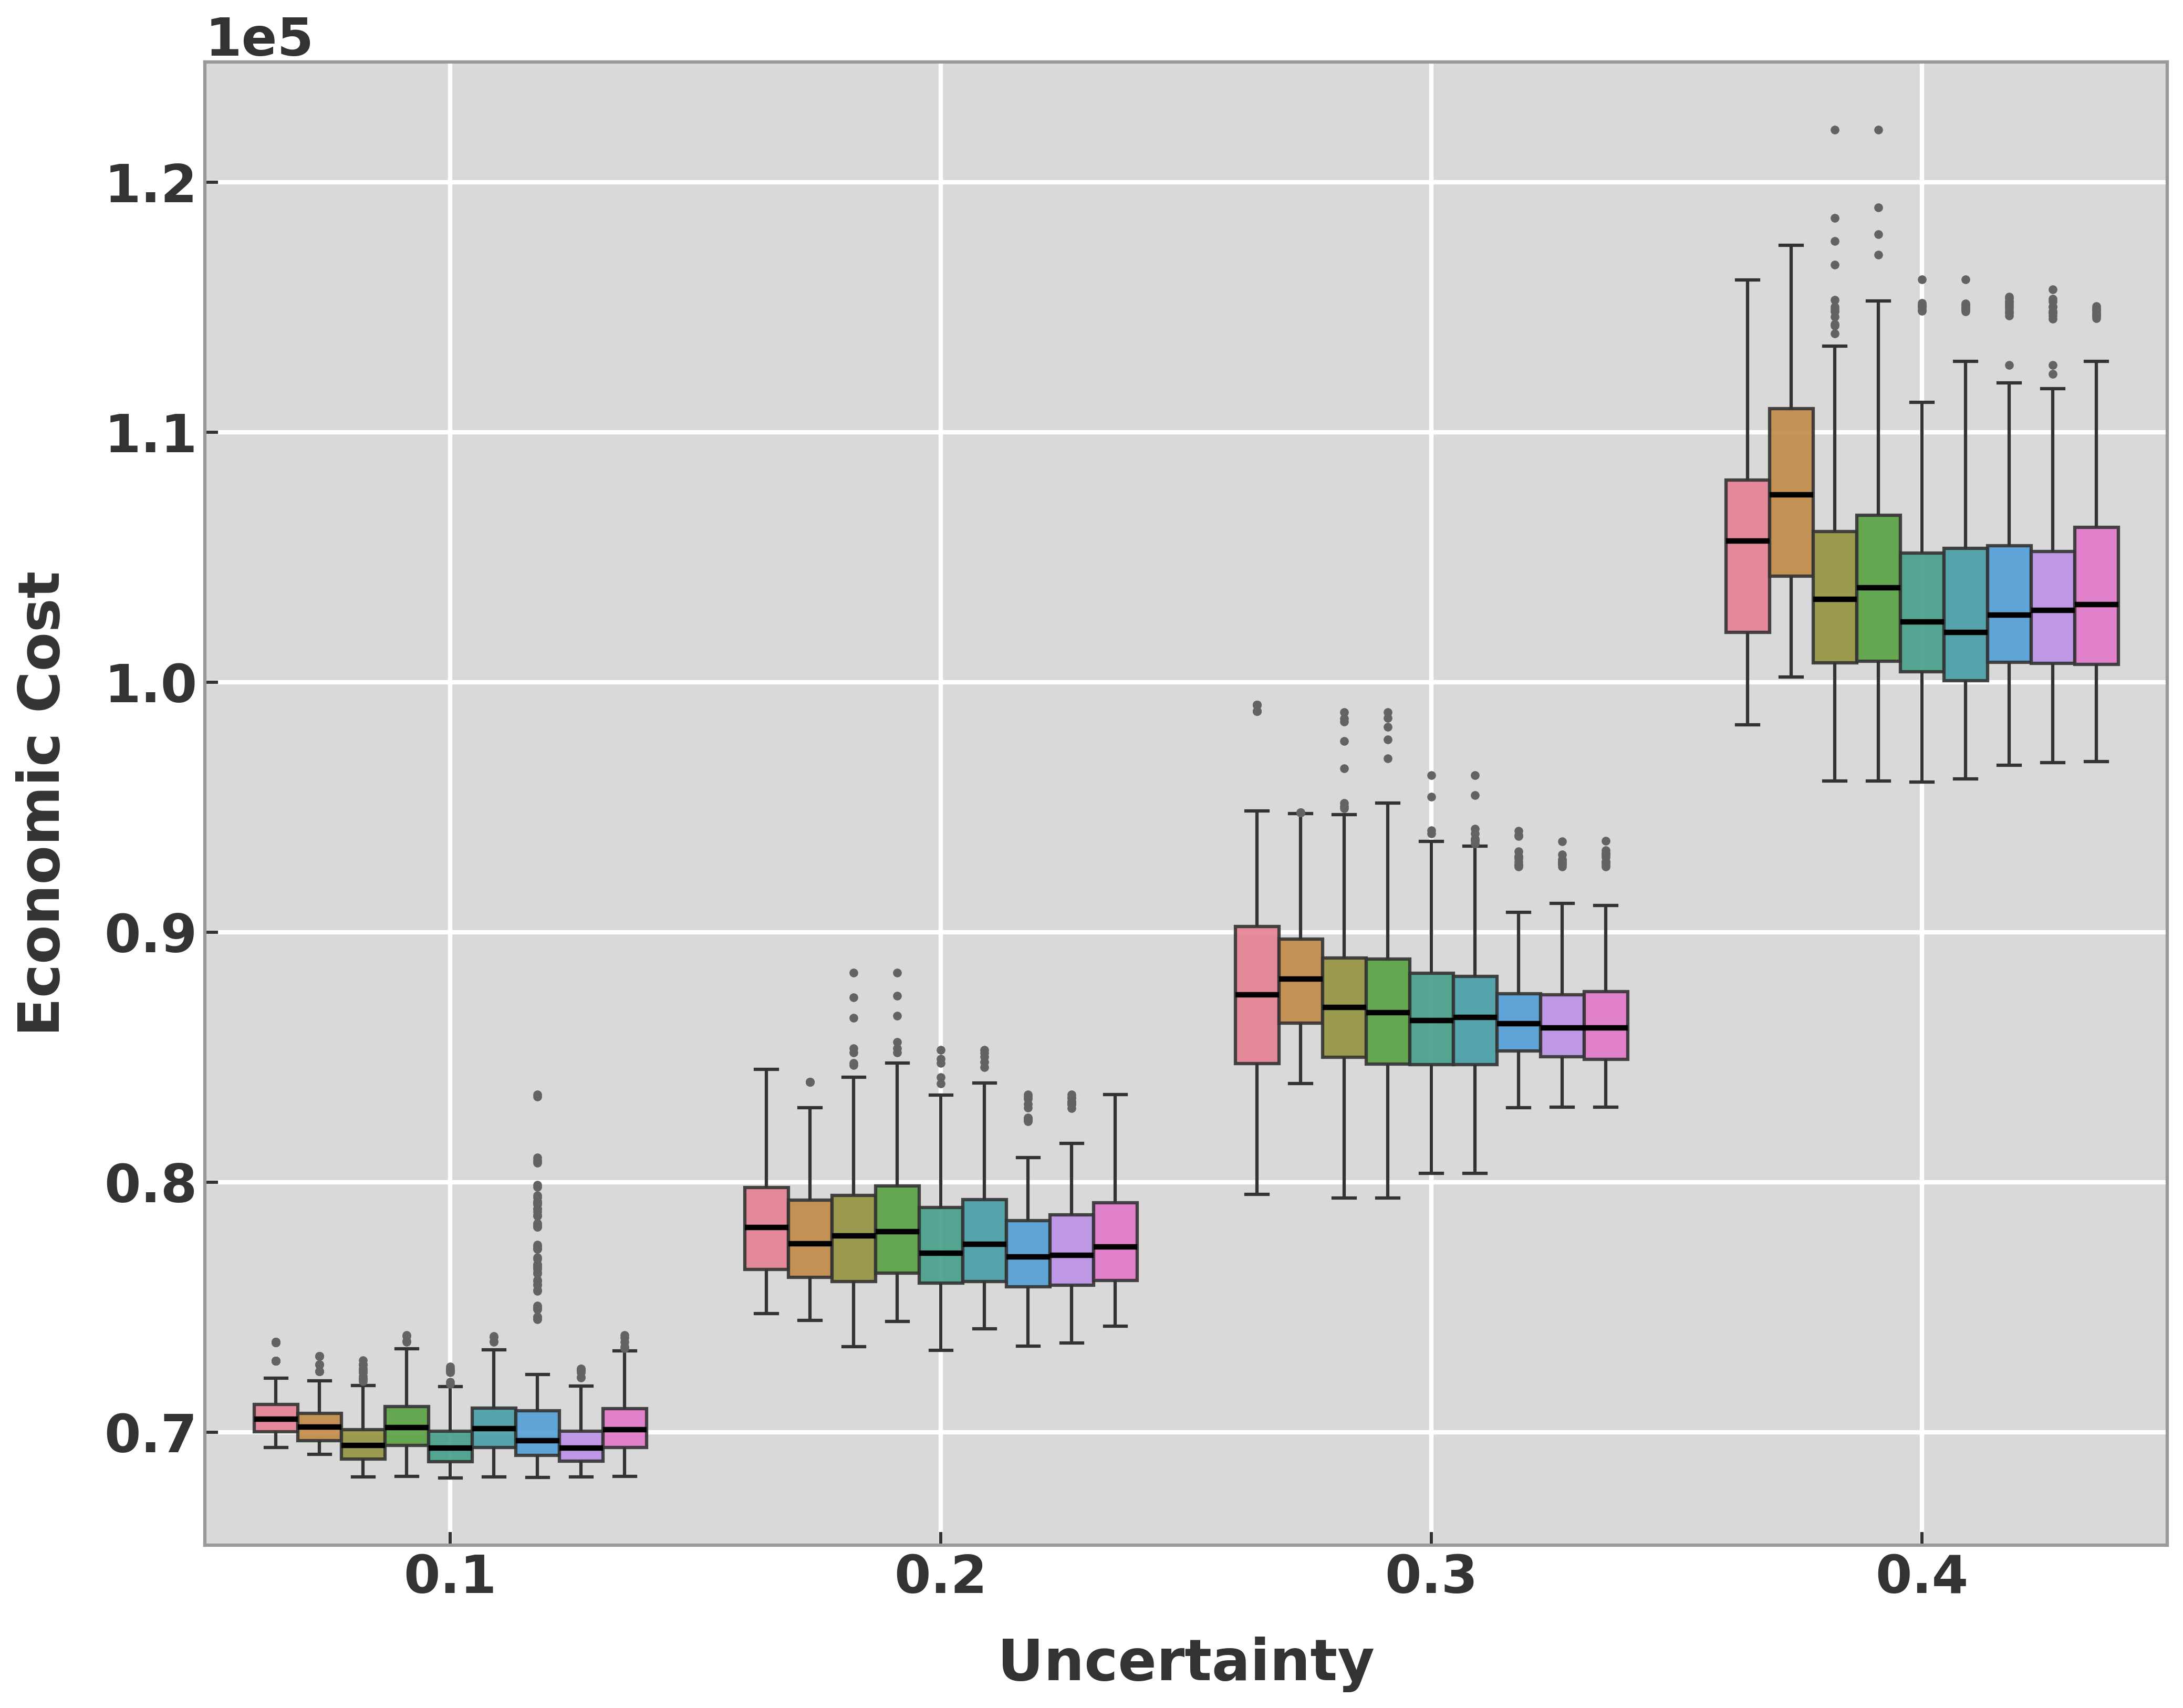
\includegraphics[width=0.45\textwidth]{figures/Traffic_0.9/traffic_0.9_economic_cost.png}
    }
    
    % Row 2
    \subfloat[Traffic density = 1.0\label{fig:ec_c}]{
        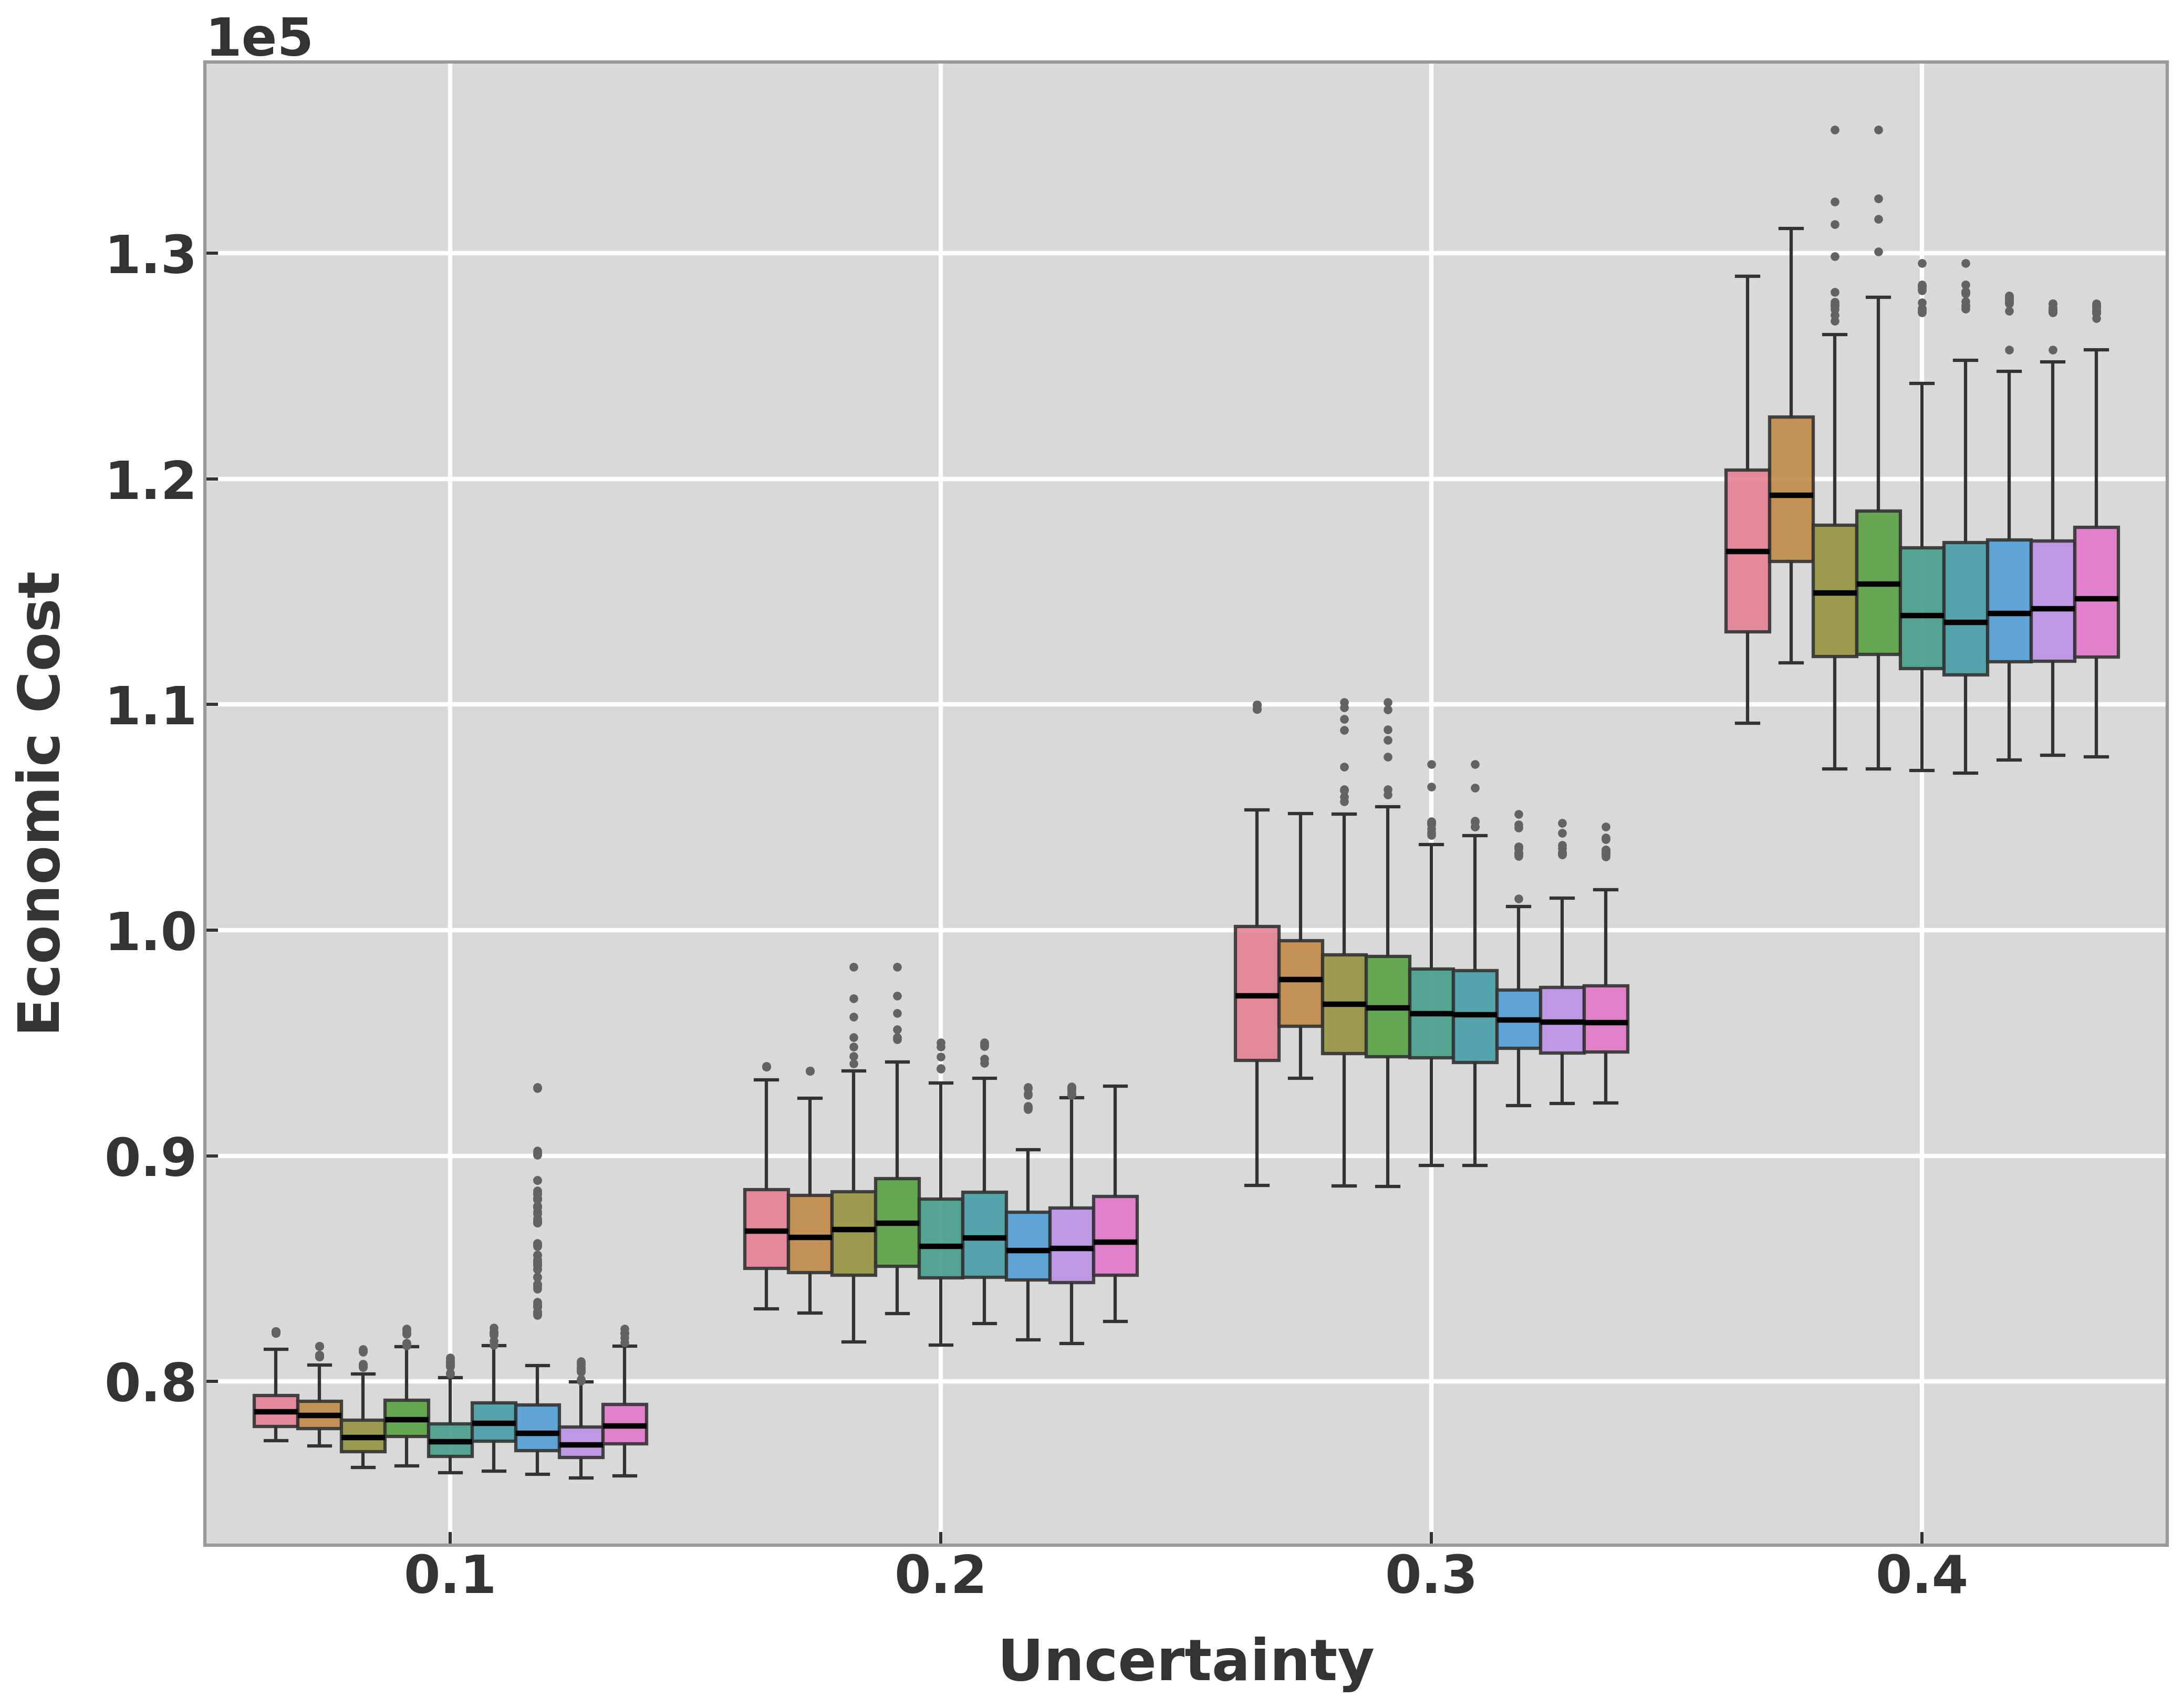
\includegraphics[width=0.45\textwidth]{figures/Traffic_1.0/traffic_1.0_economic_cost.png}
    }
    \hfill
    \subfloat[Traffic density = 1.1\label{fig:ec_d}]{
        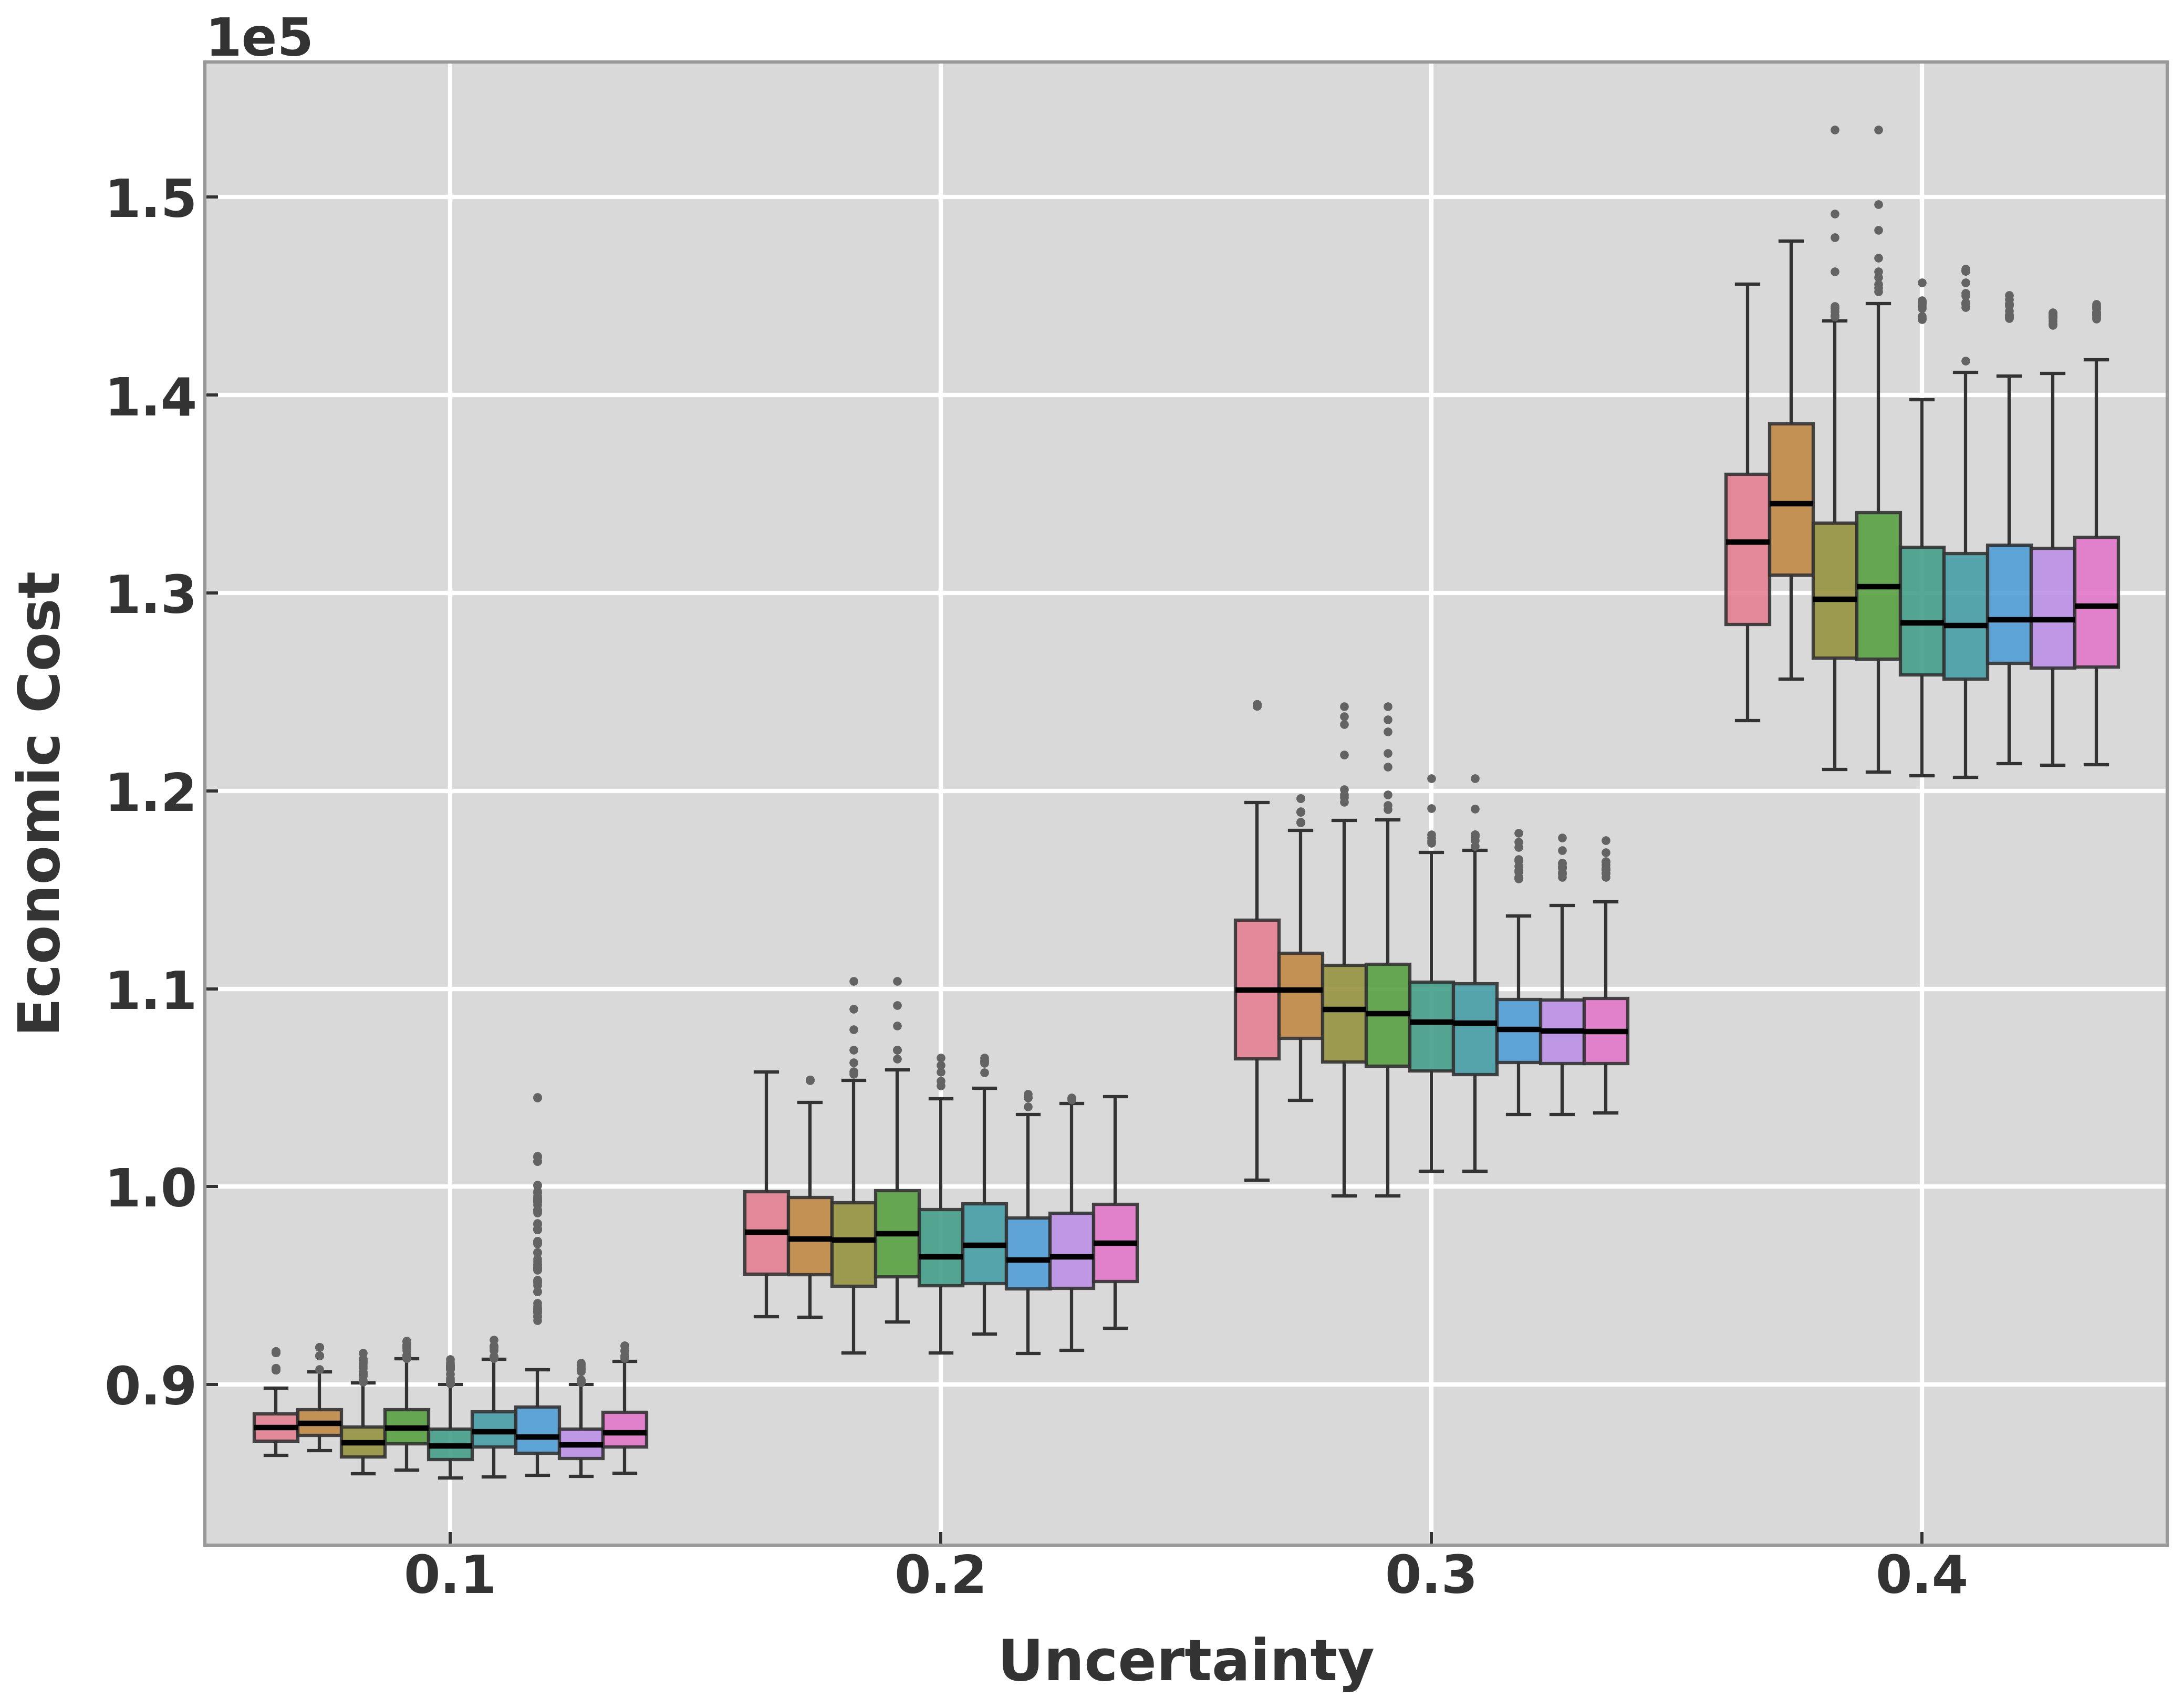
\includegraphics[width=0.45\textwidth]{figures/Traffic_1.1/traffic_1.1_economic_cost.png}
    }
    
    % Row 3 (centered single image)
    \centering
    \subfloat[Traffic density = 1.2\label{fig:ec_e}]{
        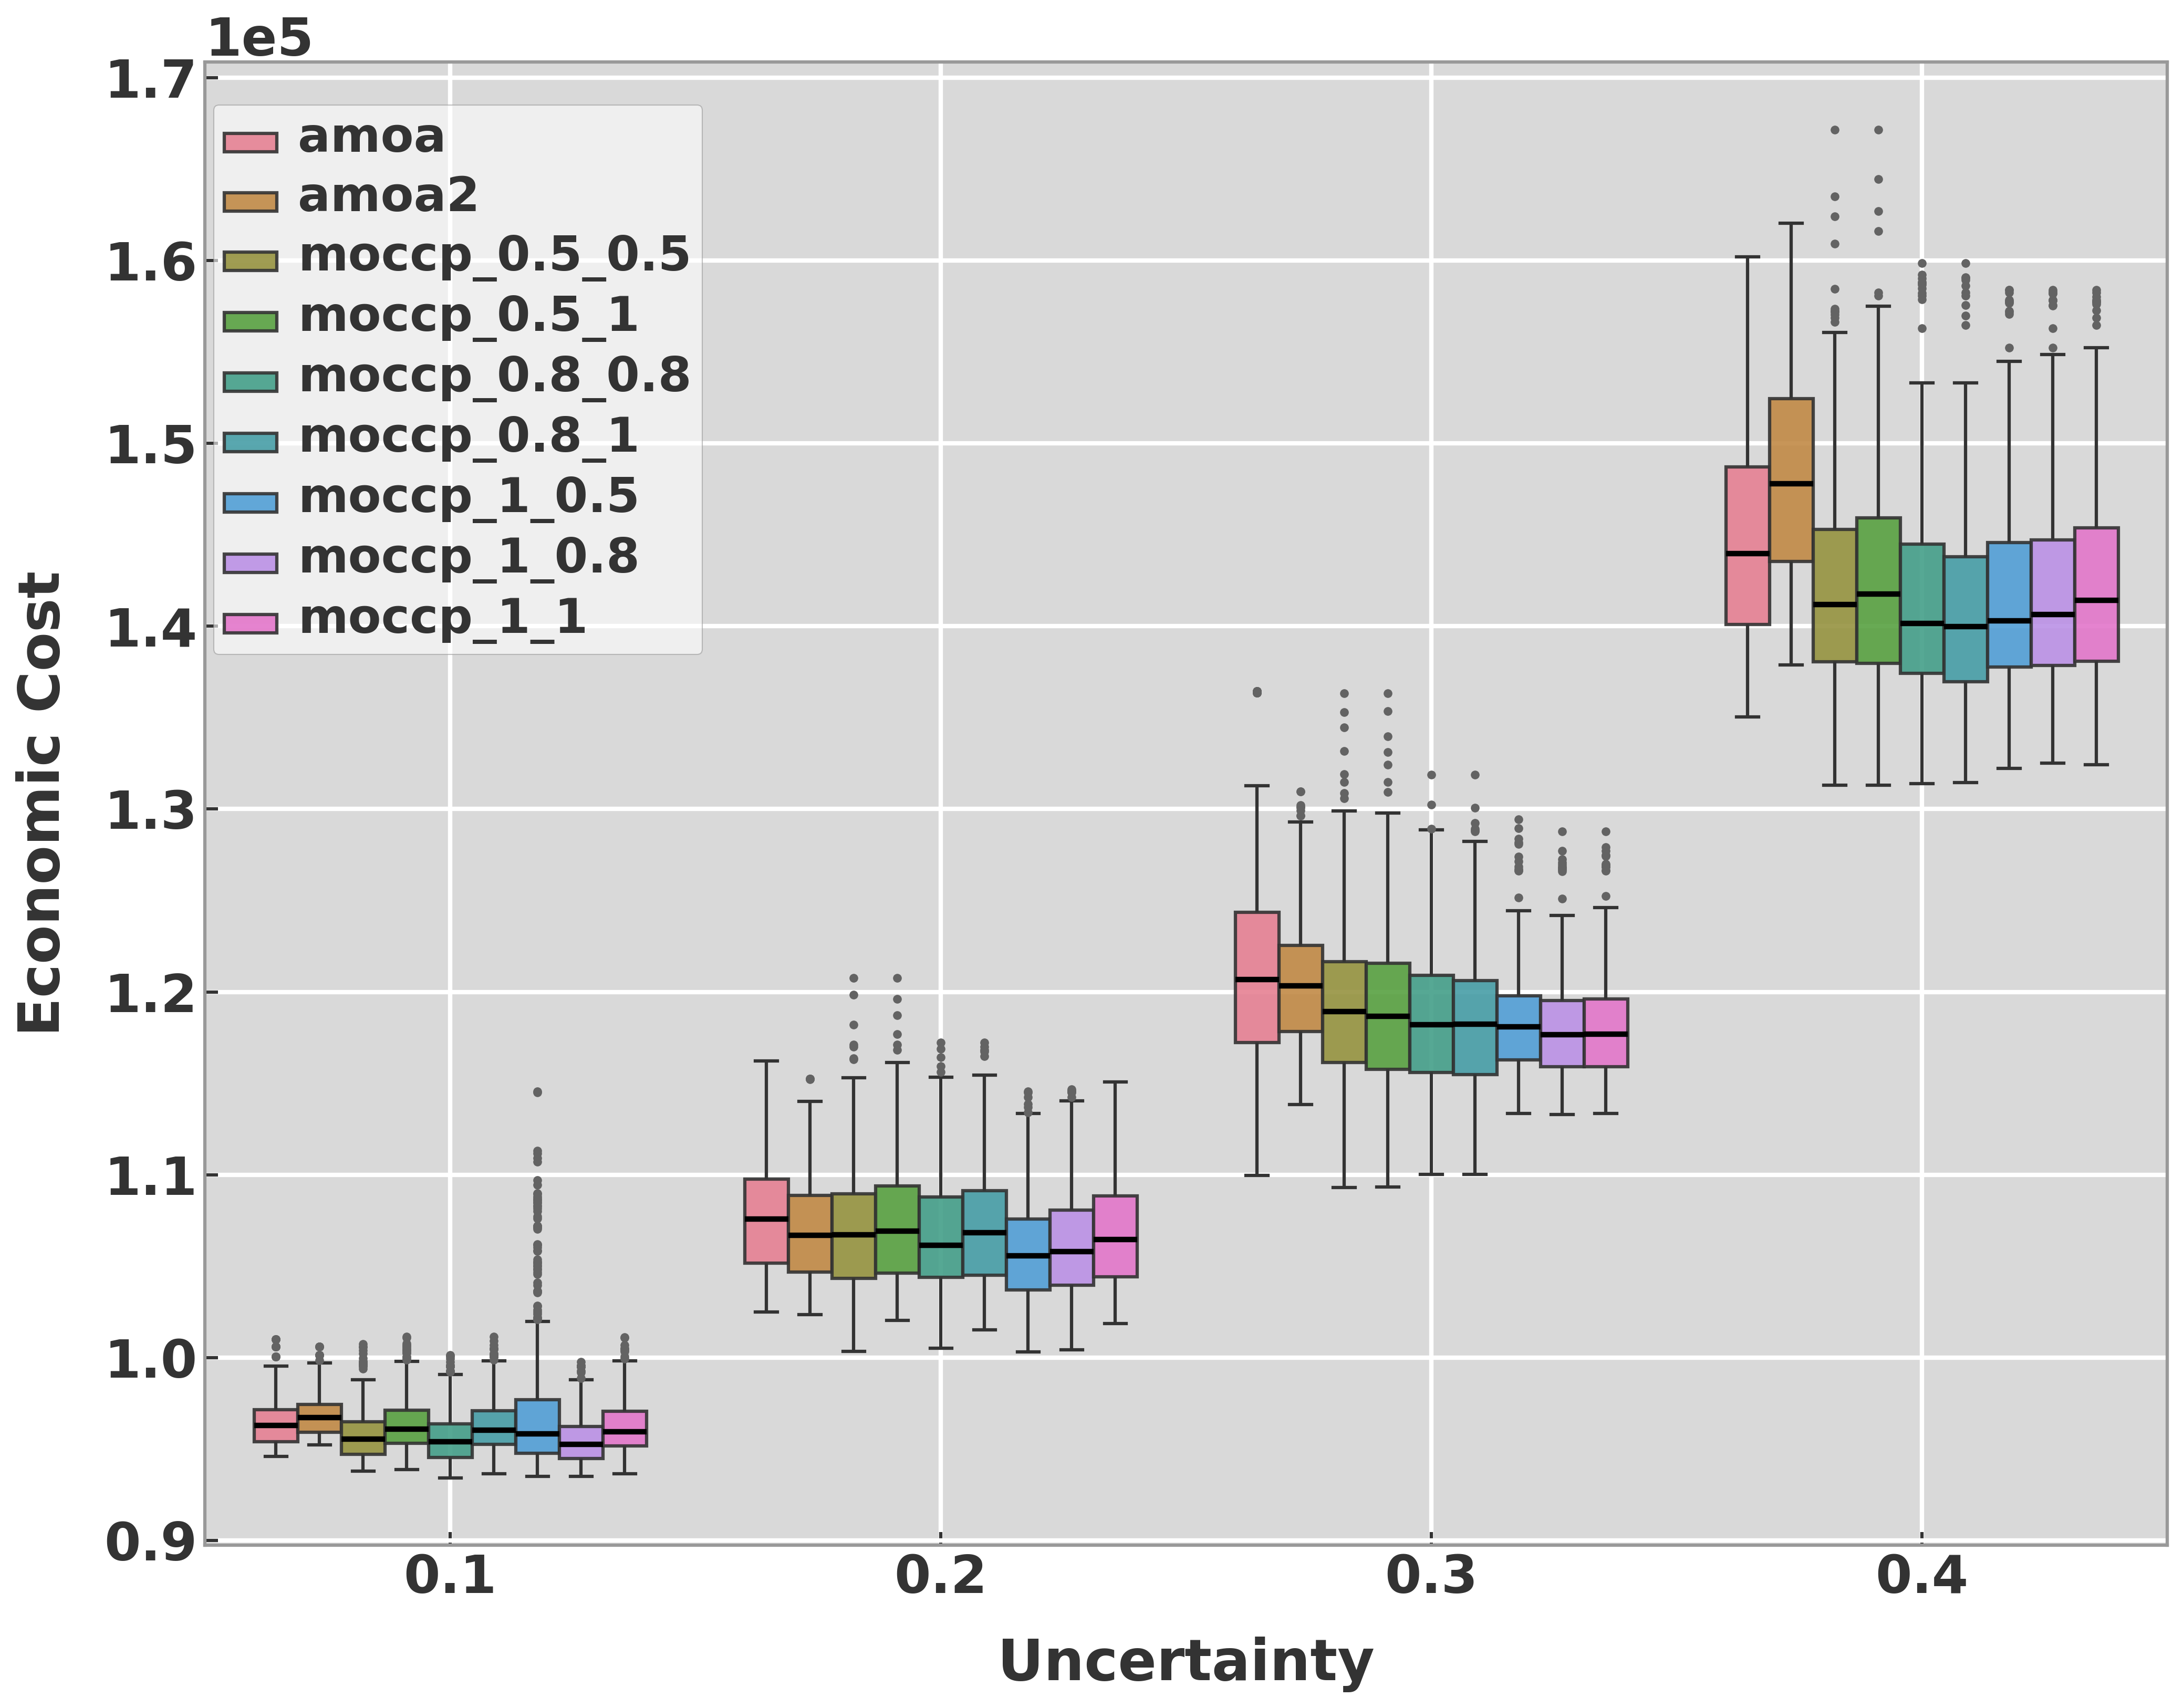
\includegraphics[width=0.45\textwidth]{figures/Traffic_1.2/traffic_1.2_economic_cost.png}
    }
    
    \caption{Economic cost under different traffic densities. Sub figures (a)–(e) correspond to traffic densities of 0.8, 0.9, 1.0, 1.1, and 1.2, respectively. And in each sub figure, each group of nine bars has the same level of uncertainties.}
    \label{fig:ec}
\end{figure}


Figs.~\ref{fig:tt} and~\ref{fig:fc} present the distributions of taxiing time and fuel consumption, respectively, across uncertainty levels from 0.1 to 0.4 and traffic densities ranging from 0.8 to 1.2. In both metrics, performance generally degrades with increasing uncertainties, with the effect amplified under higher traffic densities. The baseline algorithms (\texttt{amoa} and \texttt{amoa2}) remain competitive under low uncertainty, but their performance becomes increasingly volatile and inefficient as uncertainty grows, particularly in terms of fuel consumption. Notably, while \texttt{amoa} achieves relatively low taxiing times under an uncertainty level of 0.3, this gain is offset by a substantial increase in fuel consumption, indicating a trade-off imbalance. In contrast, the CCP-AMOA* algorithms demonstrate superior robustness across both performance metrics. Algorithms configured with higher confidence levels in taxiing time (e.g., \texttt{moccp\_1\_0.5}, \texttt{moccp\_1\_0.8}, \texttt{moccp\_1\_1}) tend to produce more stable but slightly longer taxiing time, while lower confidence levels in fuel consumption (e.g., \texttt{moccp\_1\_0.5}, \texttt{moccp\_1\_0.8}) effectively reduce fuel consumption with only modest increases in taxiing time. Algorithms such as \texttt{moccp\_0.8\_0.8} and \texttt{moccp\_1\_1} offer a well-balanced efficiency and robustness. Overall, \texttt{moccp\_1\_0.5} and \texttt{moccp\_1\_0.8} consistently achieve the lowest fuel consumption, accompanied by moderate increases in taxiing time, while \texttt{moccp\_0.8\_0.8} maintains both low taxiing time and fuel consumption. These algorithms perform best in terms of economic cost, as previously discussed, highlighting how different confidence levels influence the trade-off between taxiing time and fuel consumption under uncertainties.

% Taxiing Time Figure
\begin{figure}[htp]
    \centering
    
    \subfloat[Traffic density = 0.8\label{fig:tt_a}]{
        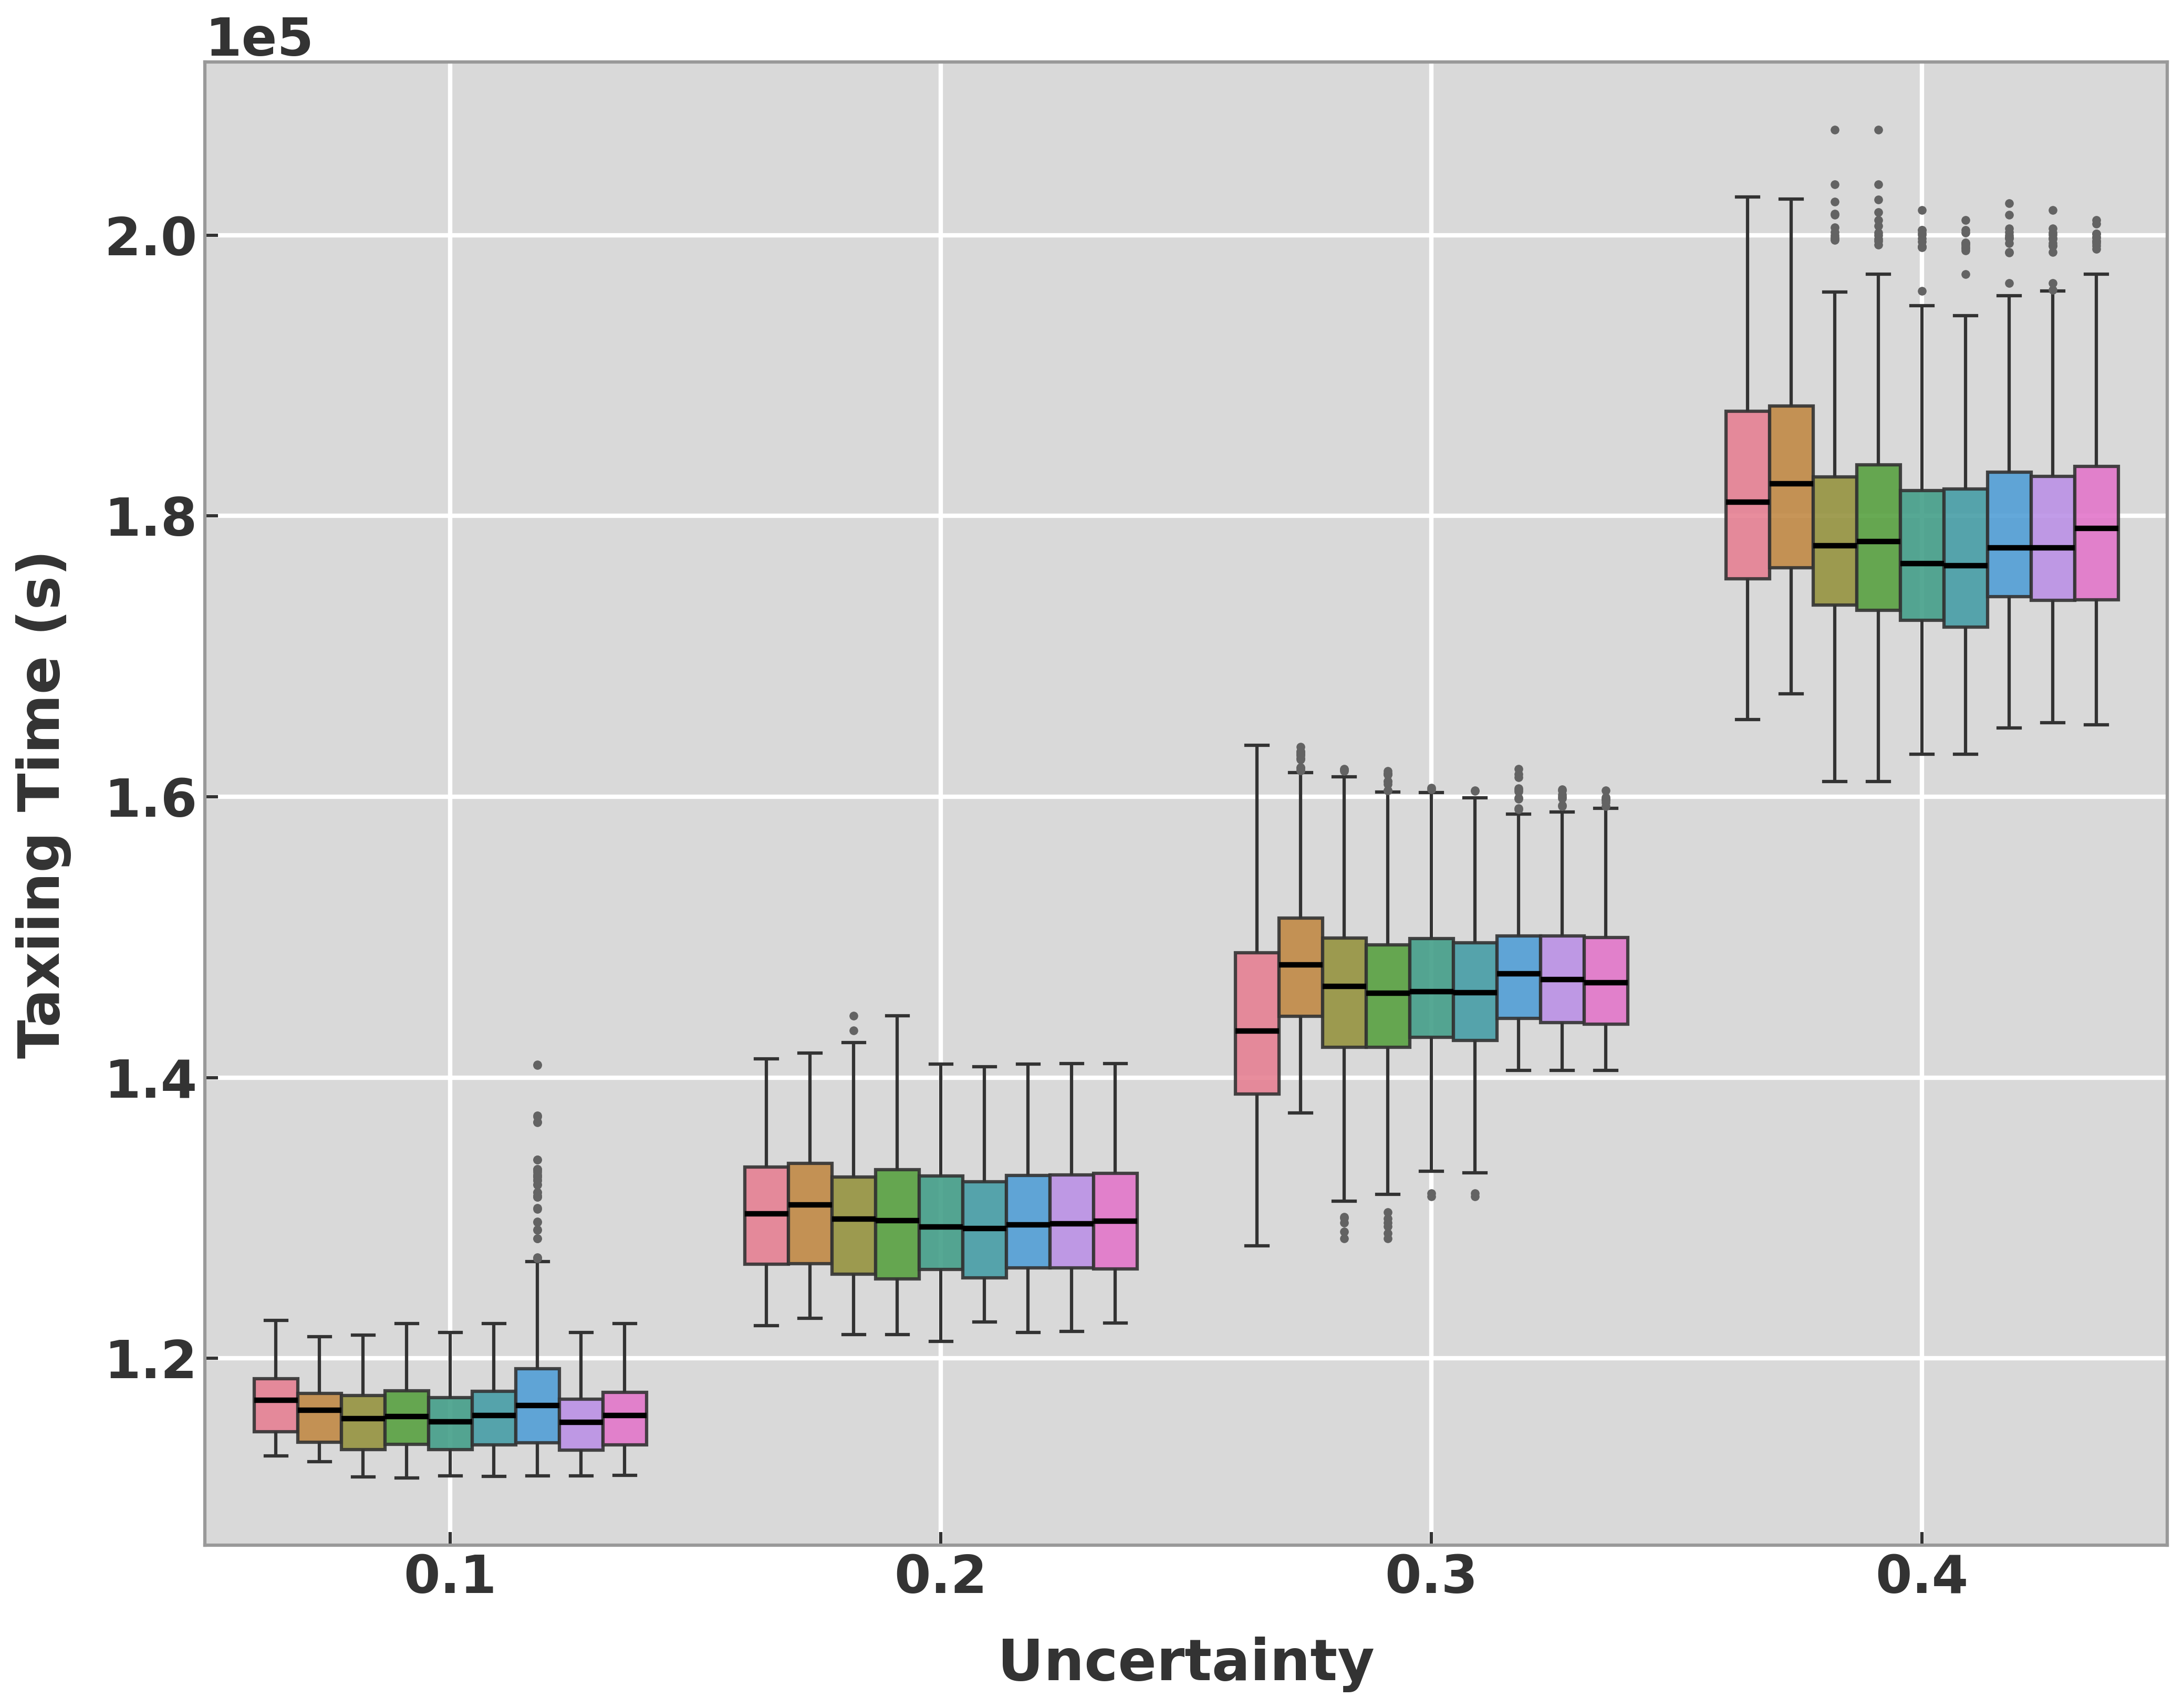
\includegraphics[width=0.45\textwidth]{figures/Traffic_0.8/traffic_0.8_taxiing_time.png}
    }
    \hfill
    \subfloat[Traffic density = 0.9\label{fig:tt_b}]{
        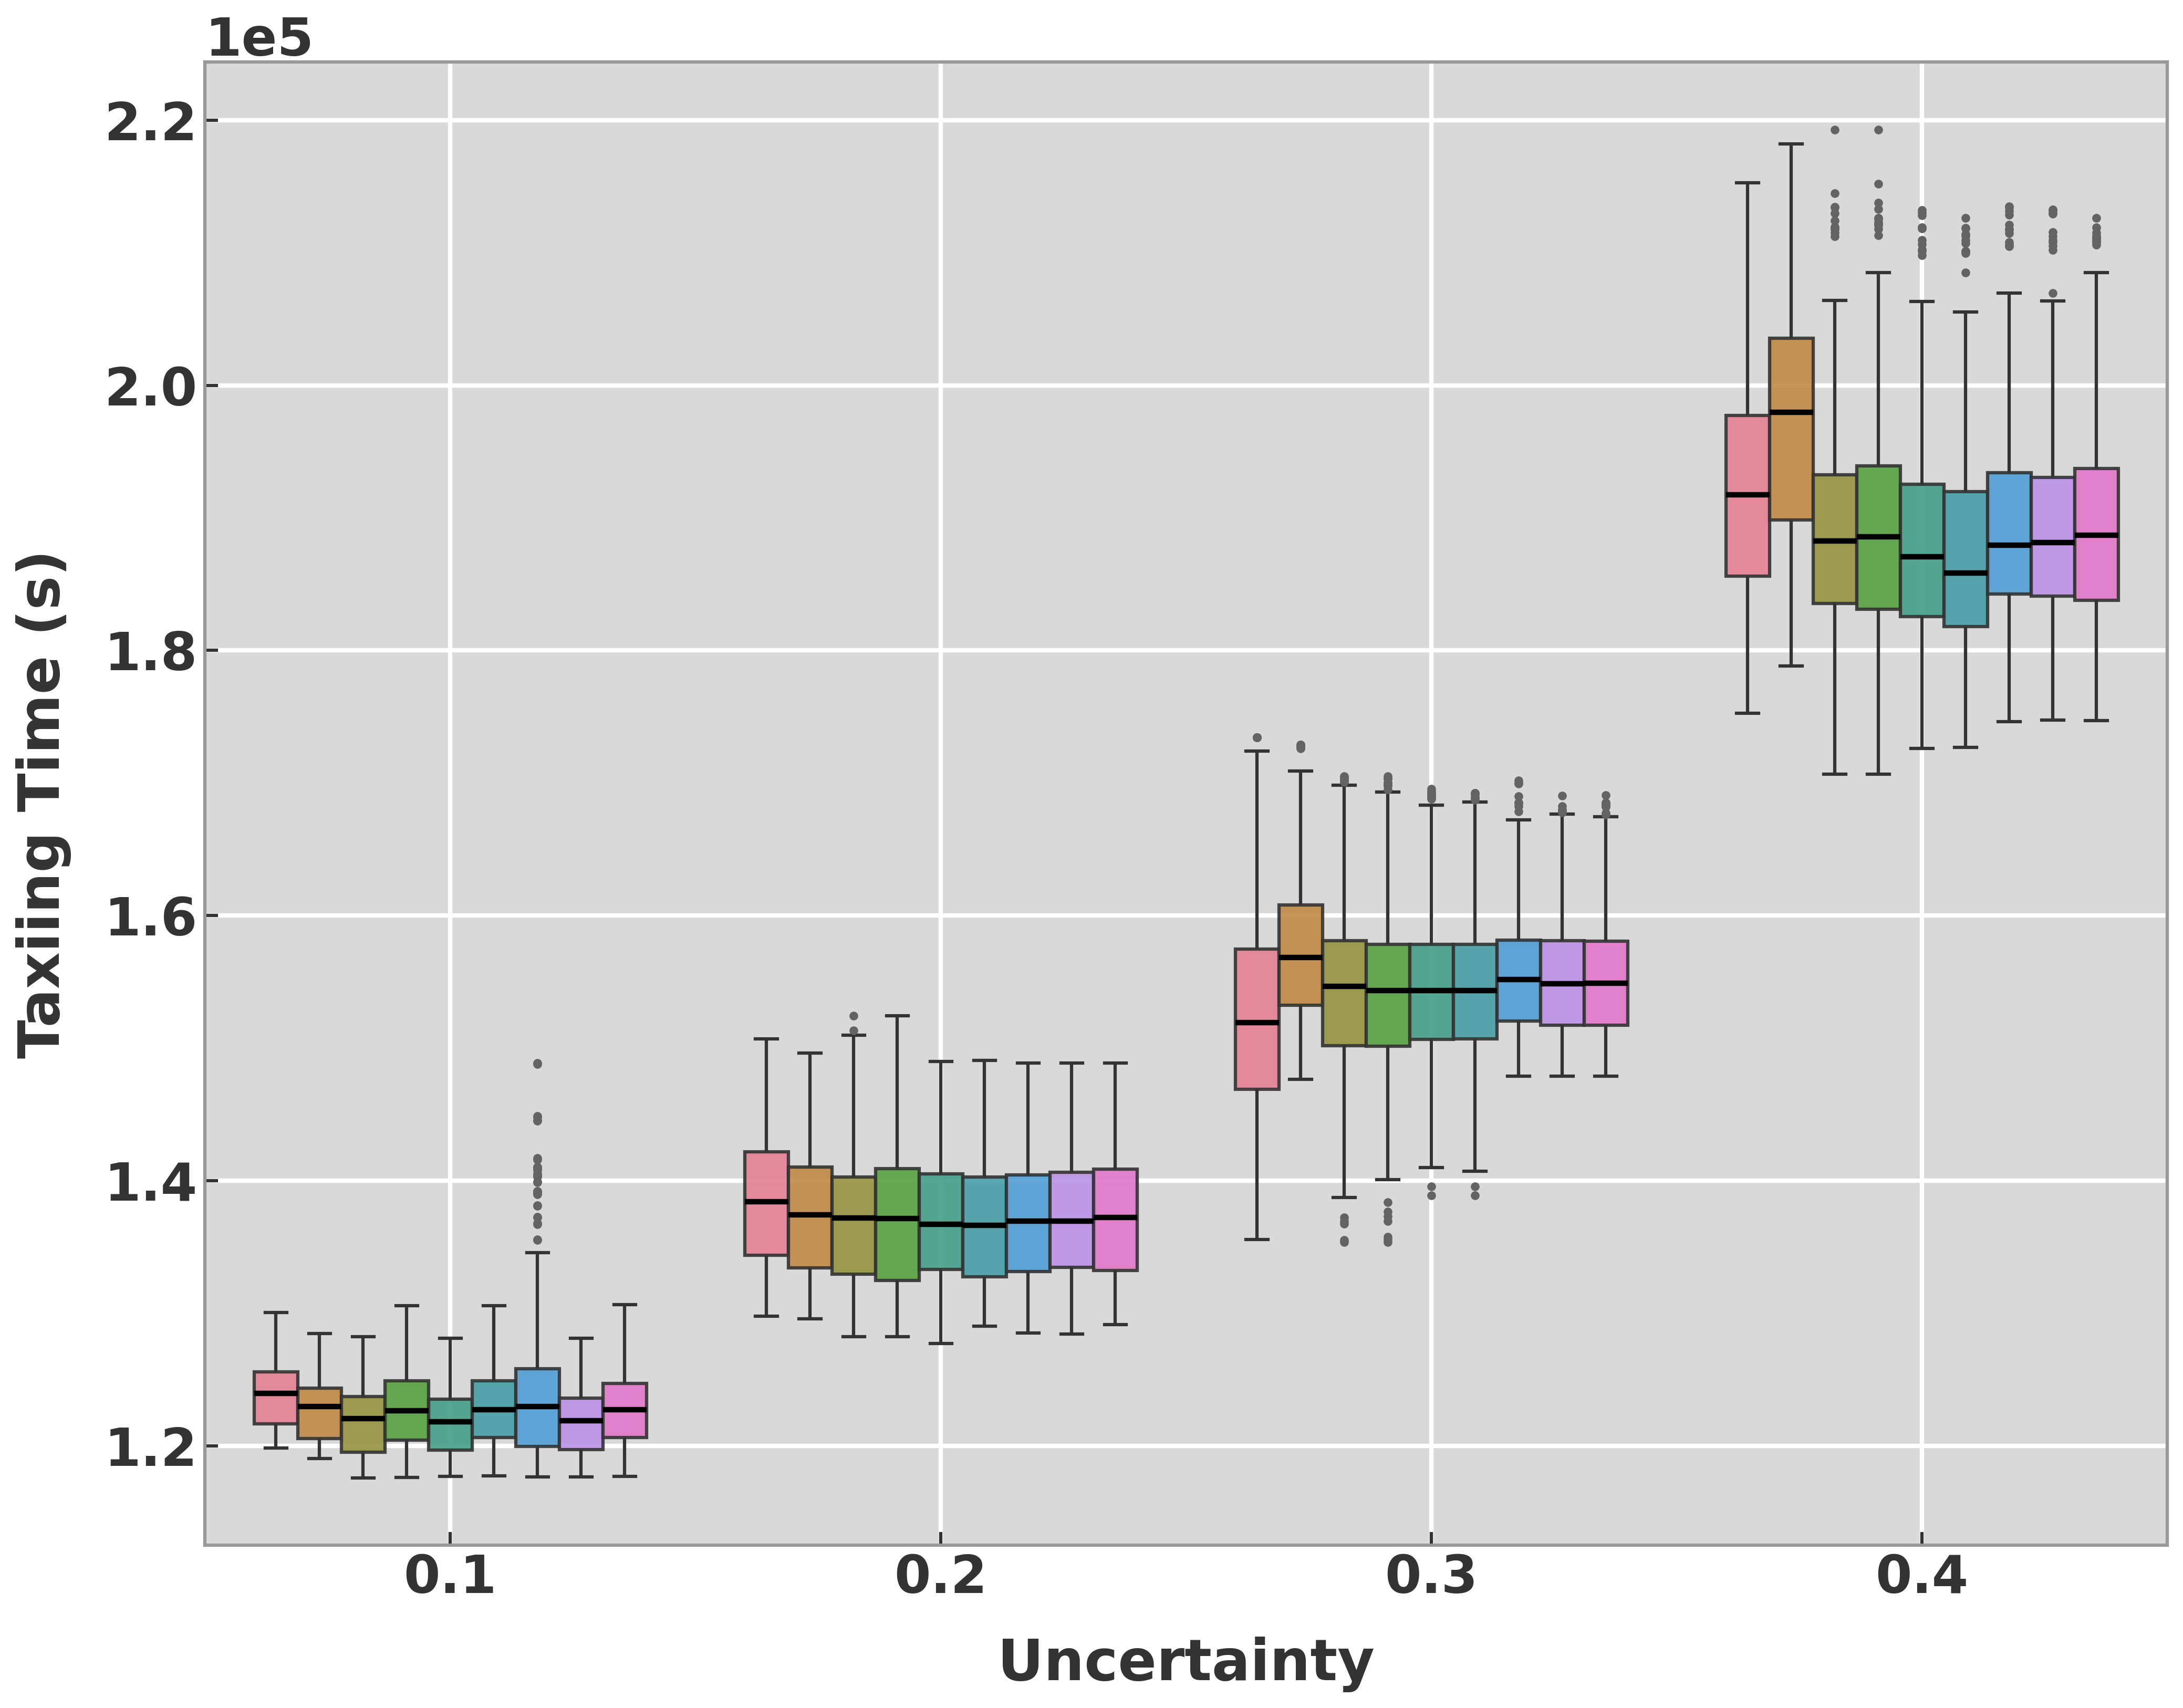
\includegraphics[width=0.45\textwidth]{figures/Traffic_0.9/traffic_0.9_taxiing_time.png}
    }
    
    \subfloat[Traffic density = 1.0\label{fig:tt_c}]{
        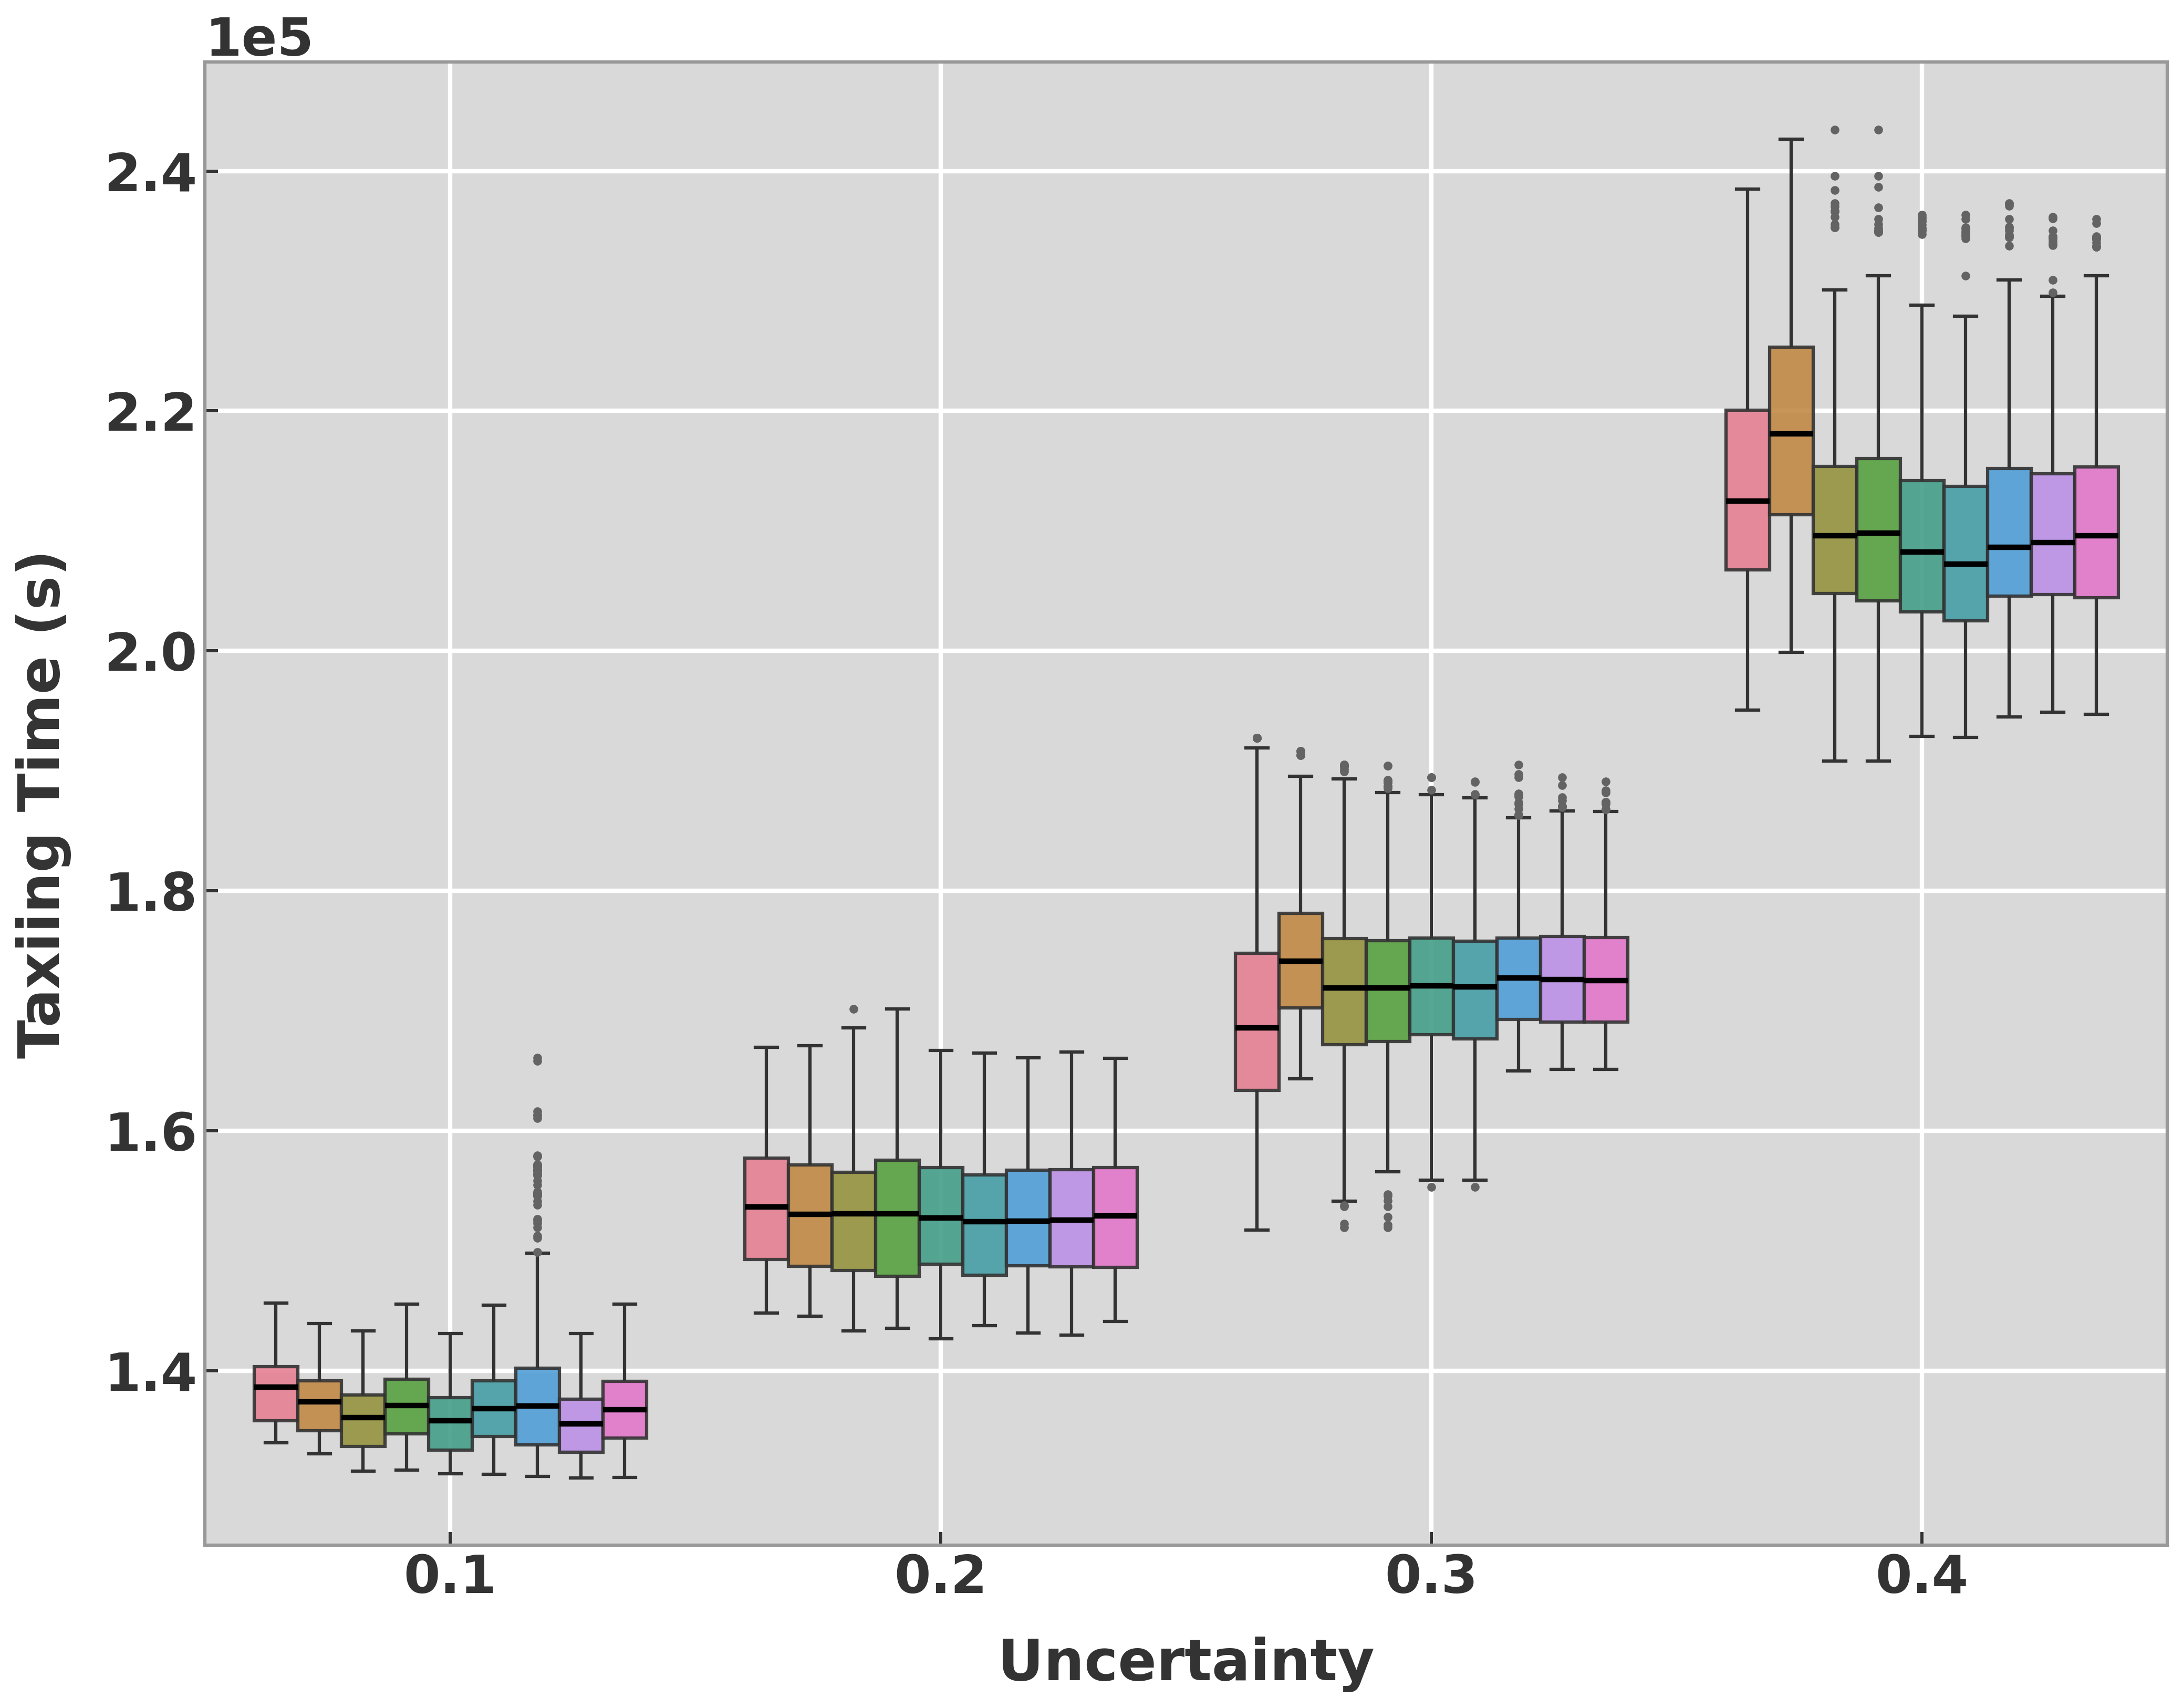
\includegraphics[width=0.45\textwidth]{figures/Traffic_1.0/traffic_1.0_taxiing_time.png}
    }
    \hfill
    \subfloat[Traffic density = 1.1\label{fig:tt_d}]{
        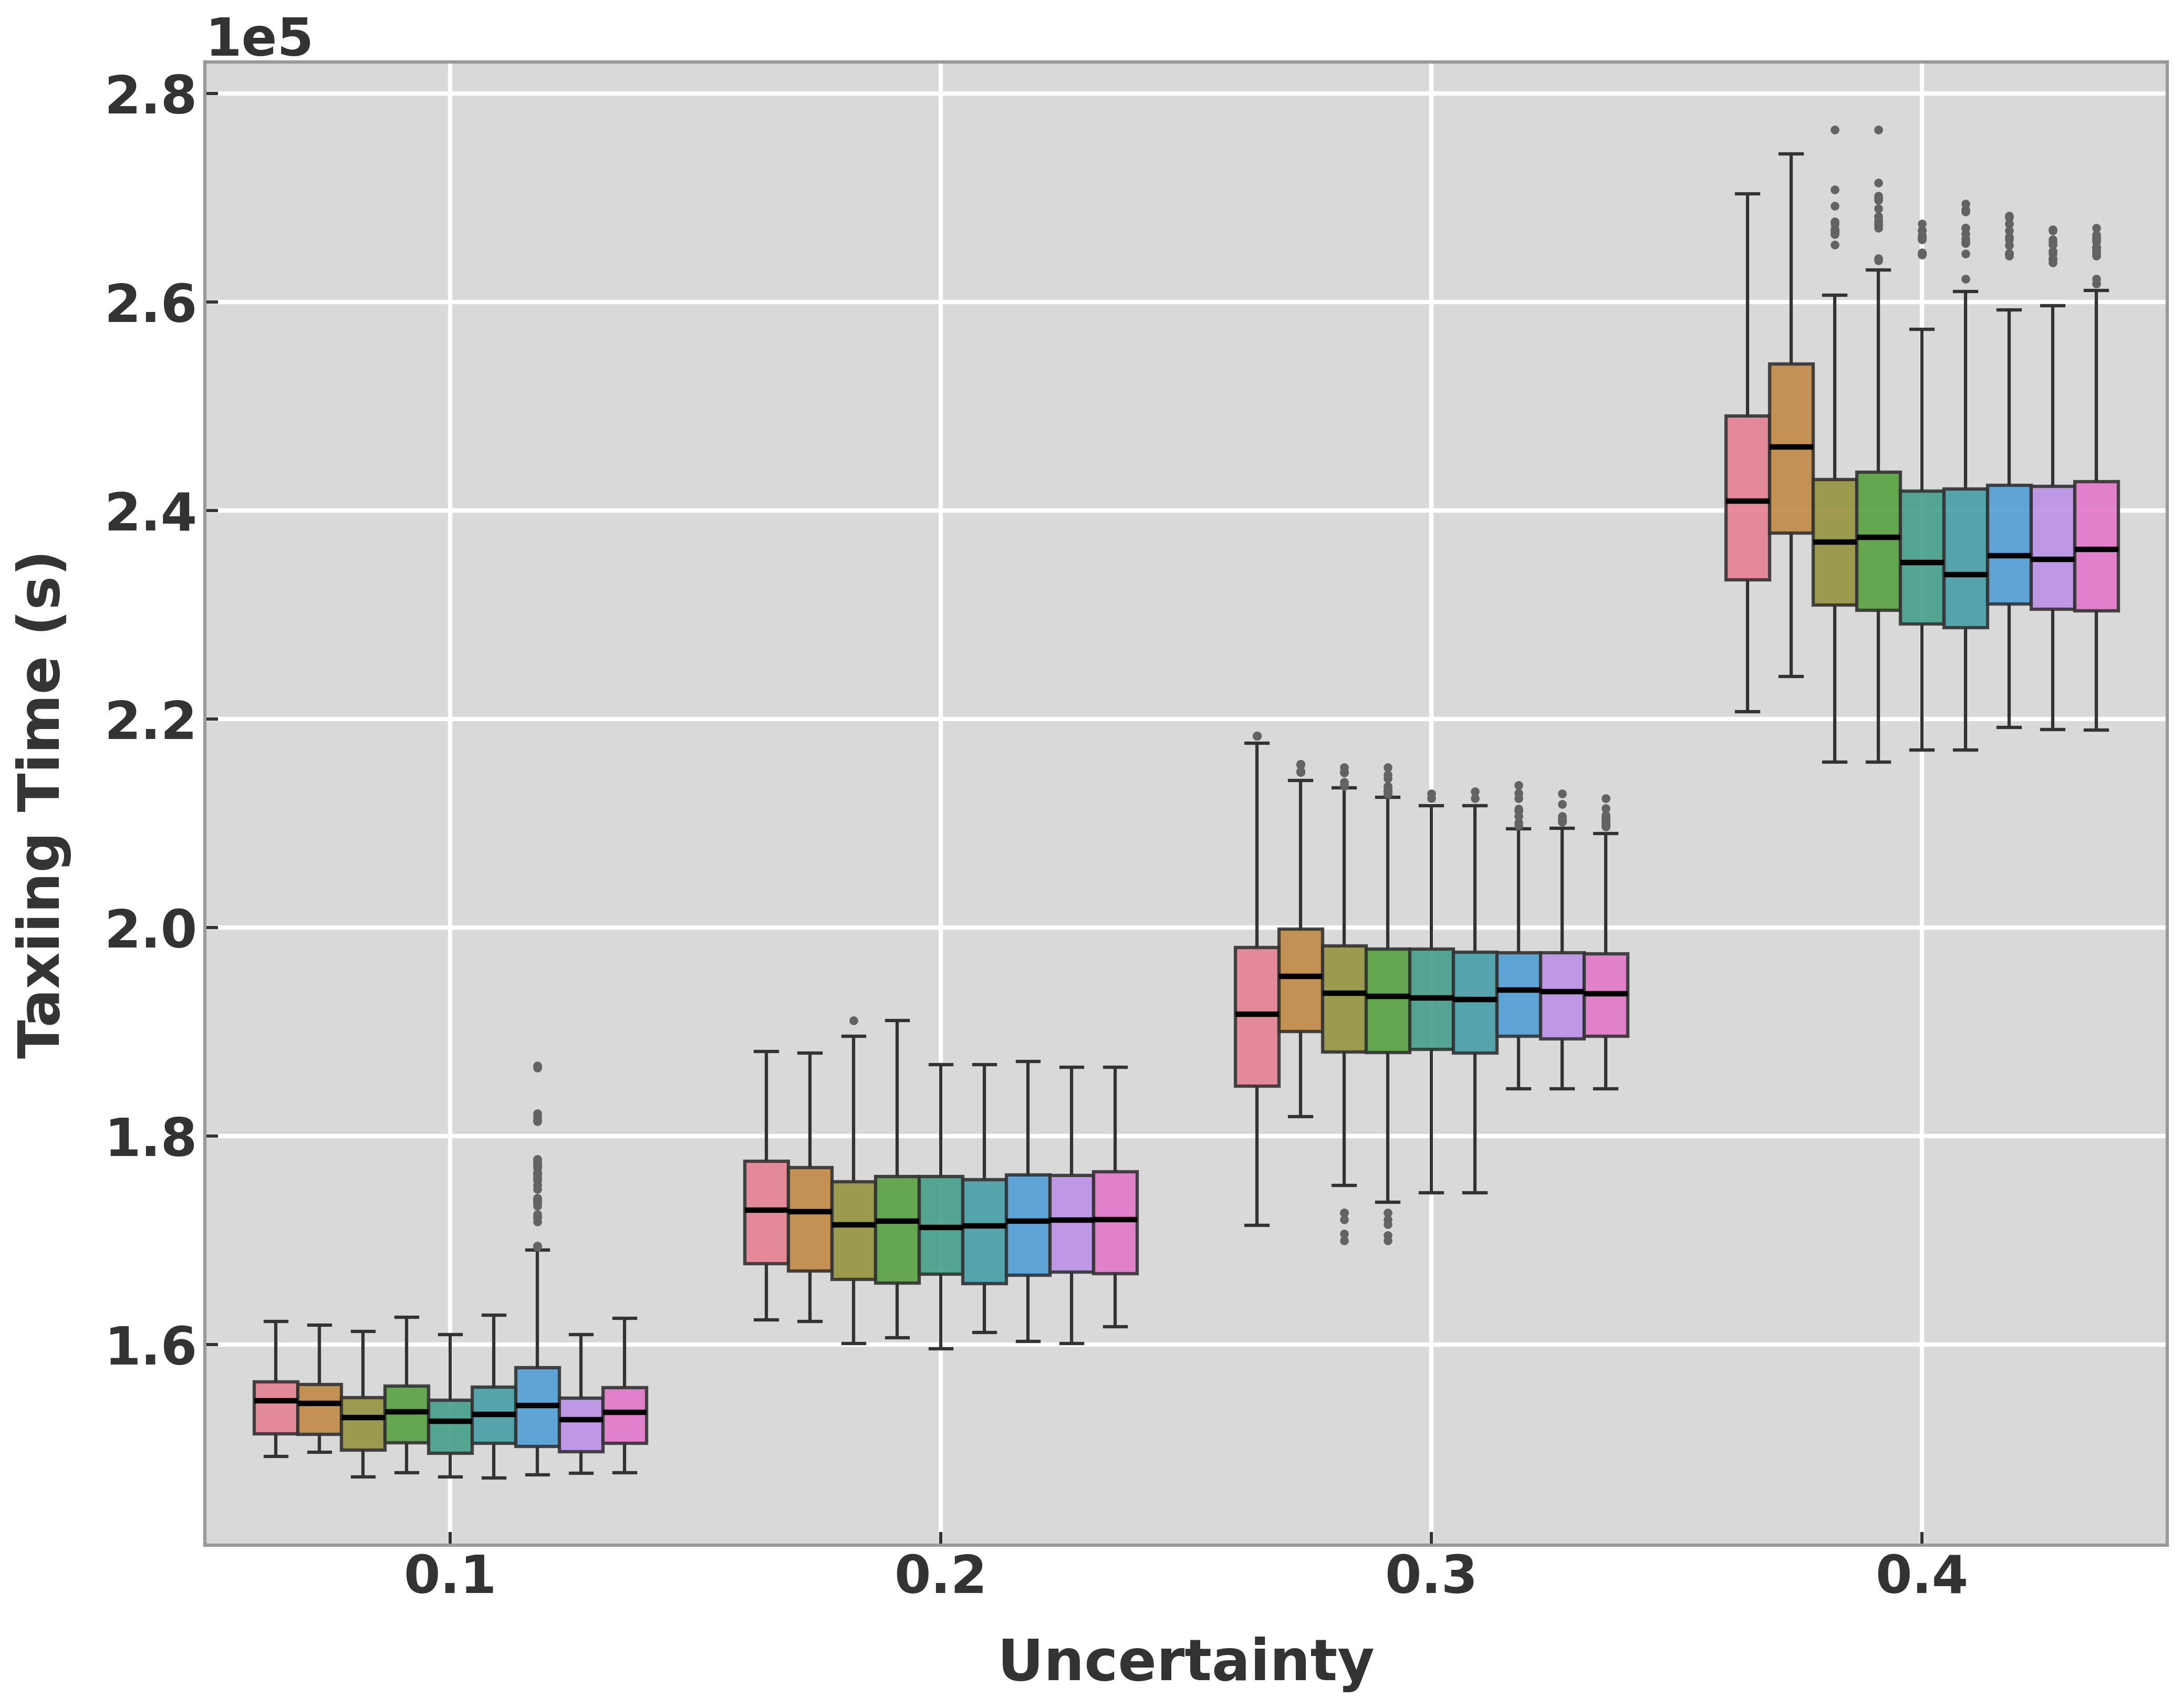
\includegraphics[width=0.45\textwidth]{figures/Traffic_1.1/traffic_1.1_taxiing_time.png}
    }
    
    \centering
    \subfloat[Traffic density = 1.2\label{fig:tt_e}]{
        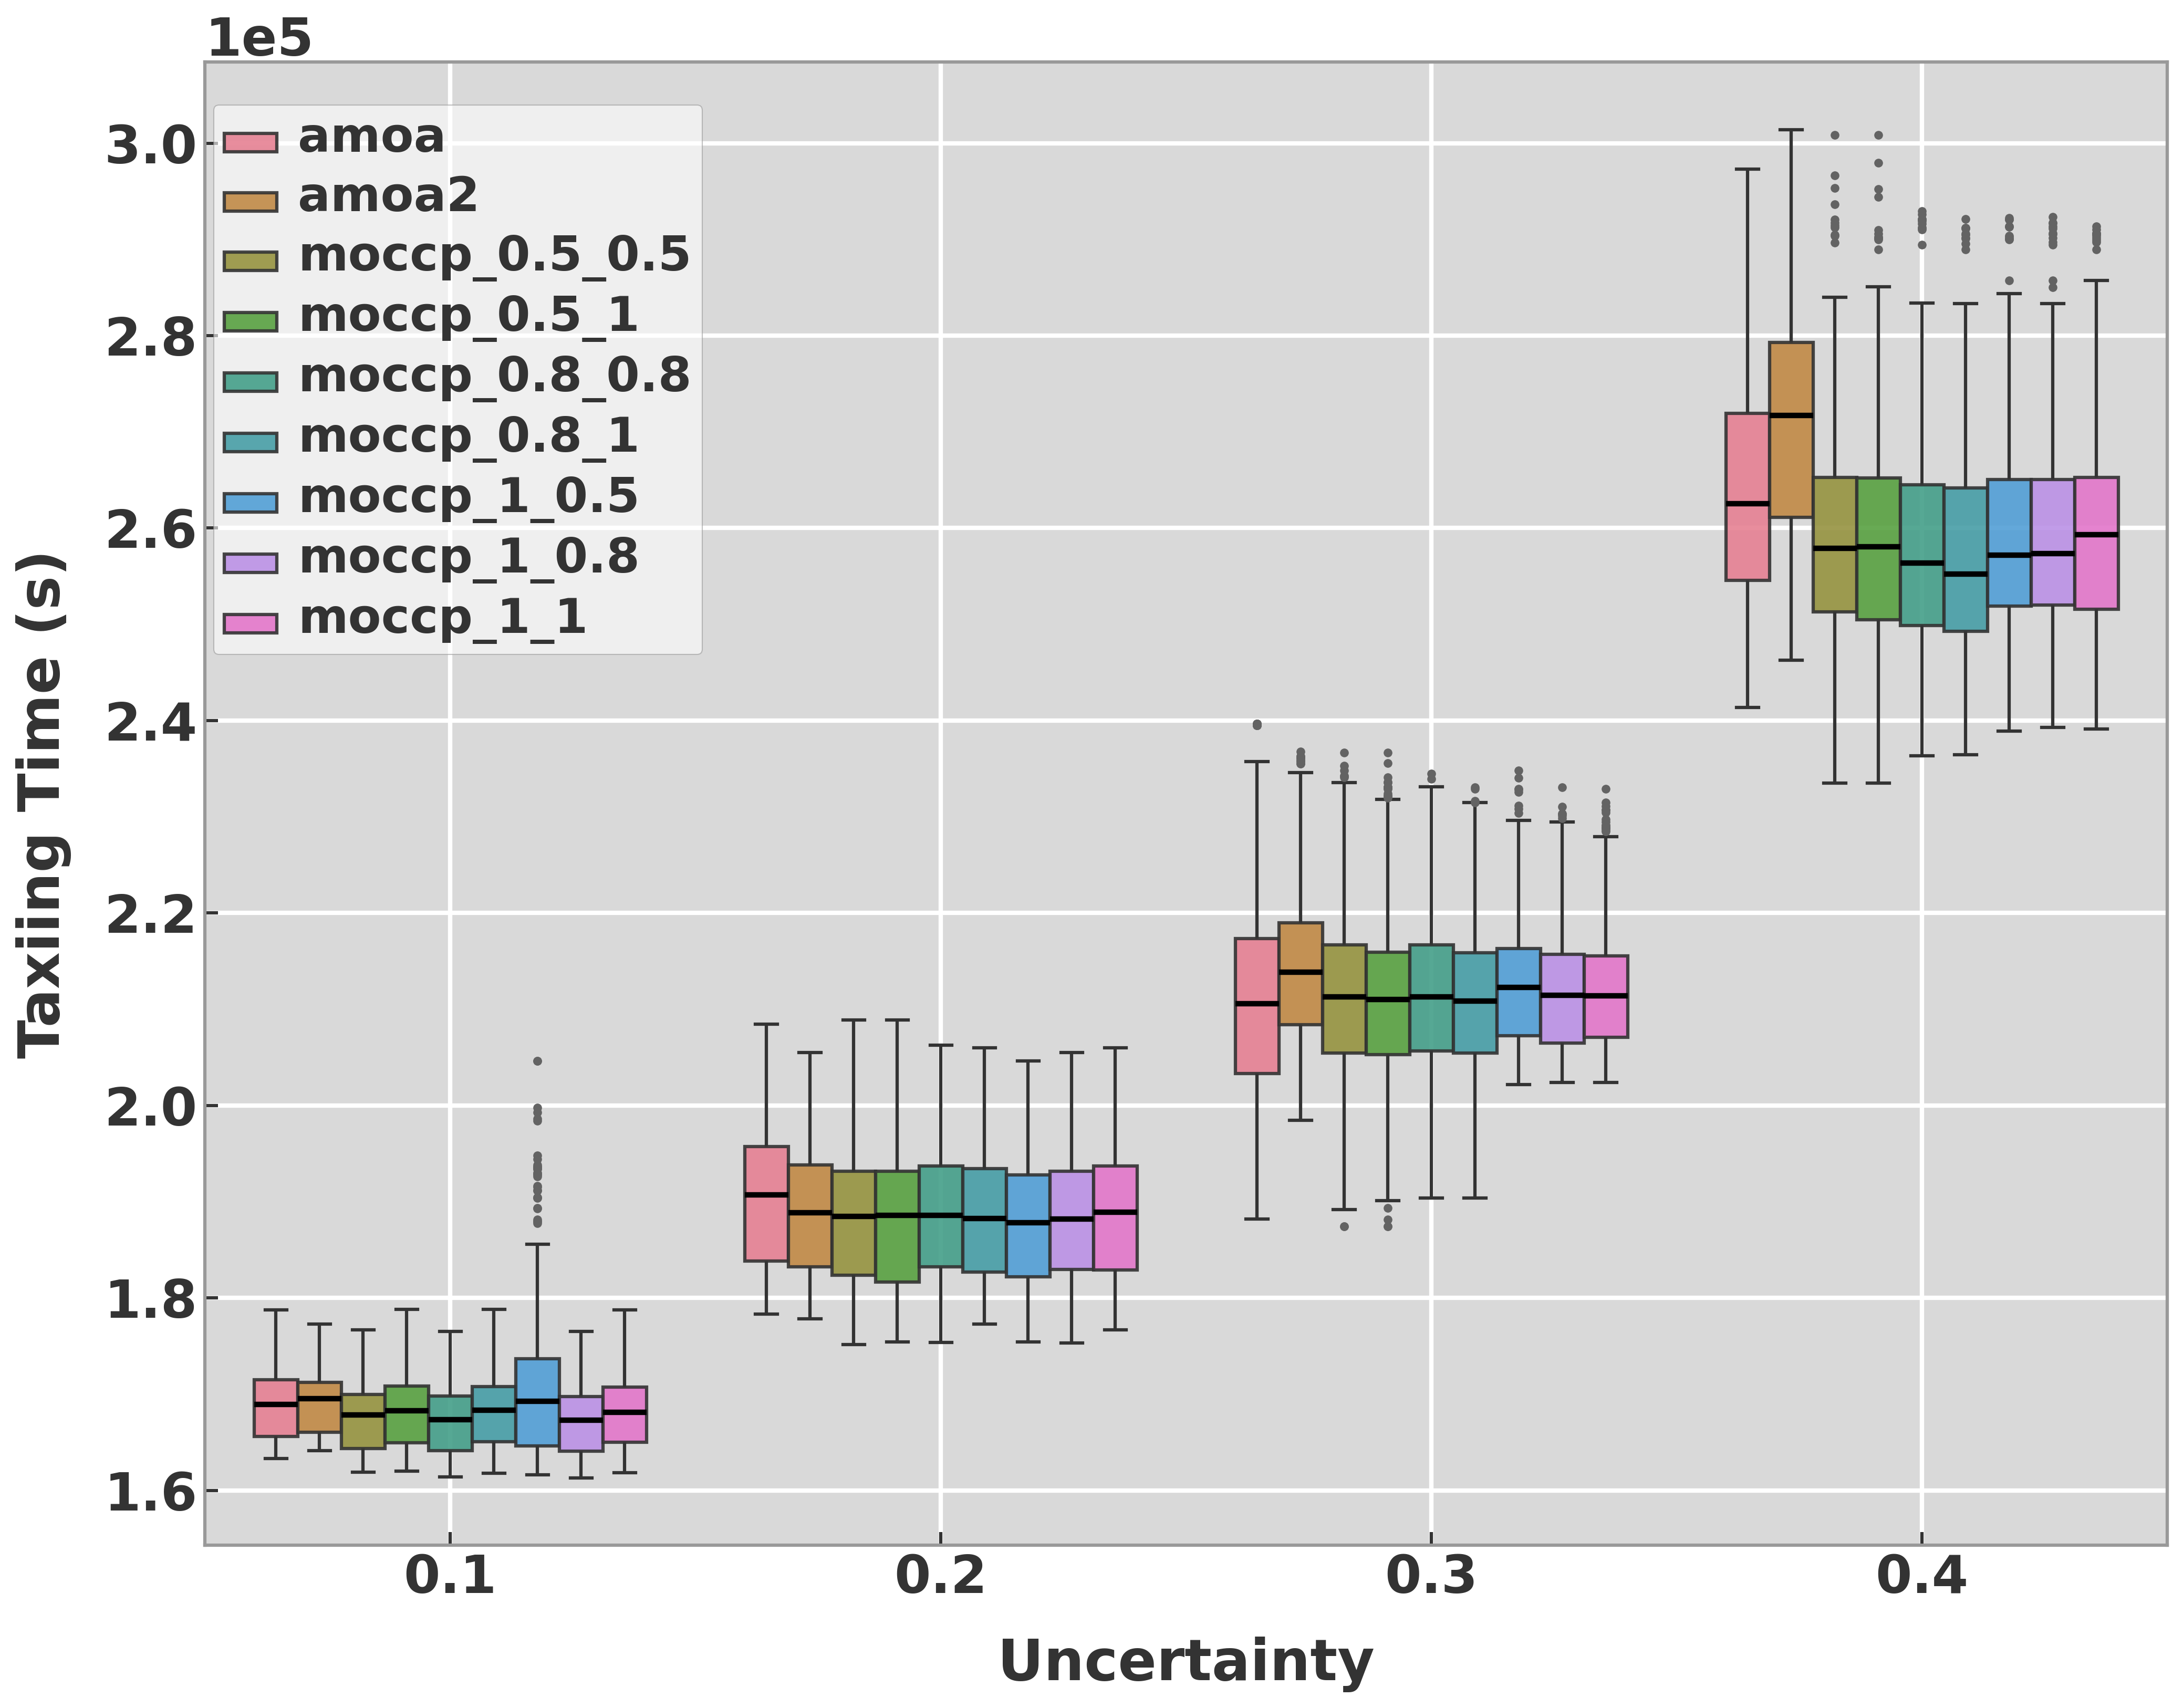
\includegraphics[width=0.45\textwidth]{figures/Traffic_1.2/traffic_1.2_taxiing_time.png}
    }
    
    \caption{Taxiing time under different traffic densities. In each sub figure, each group of nine bars has the same level of uncertainties.}
    \label{fig:tt}
\end{figure}

% Fuel Consumption Figure
\begin{figure}[htp]
    \centering
    
    \subfloat[Traffic density = 0.8\label{fig:fc_a}]{
        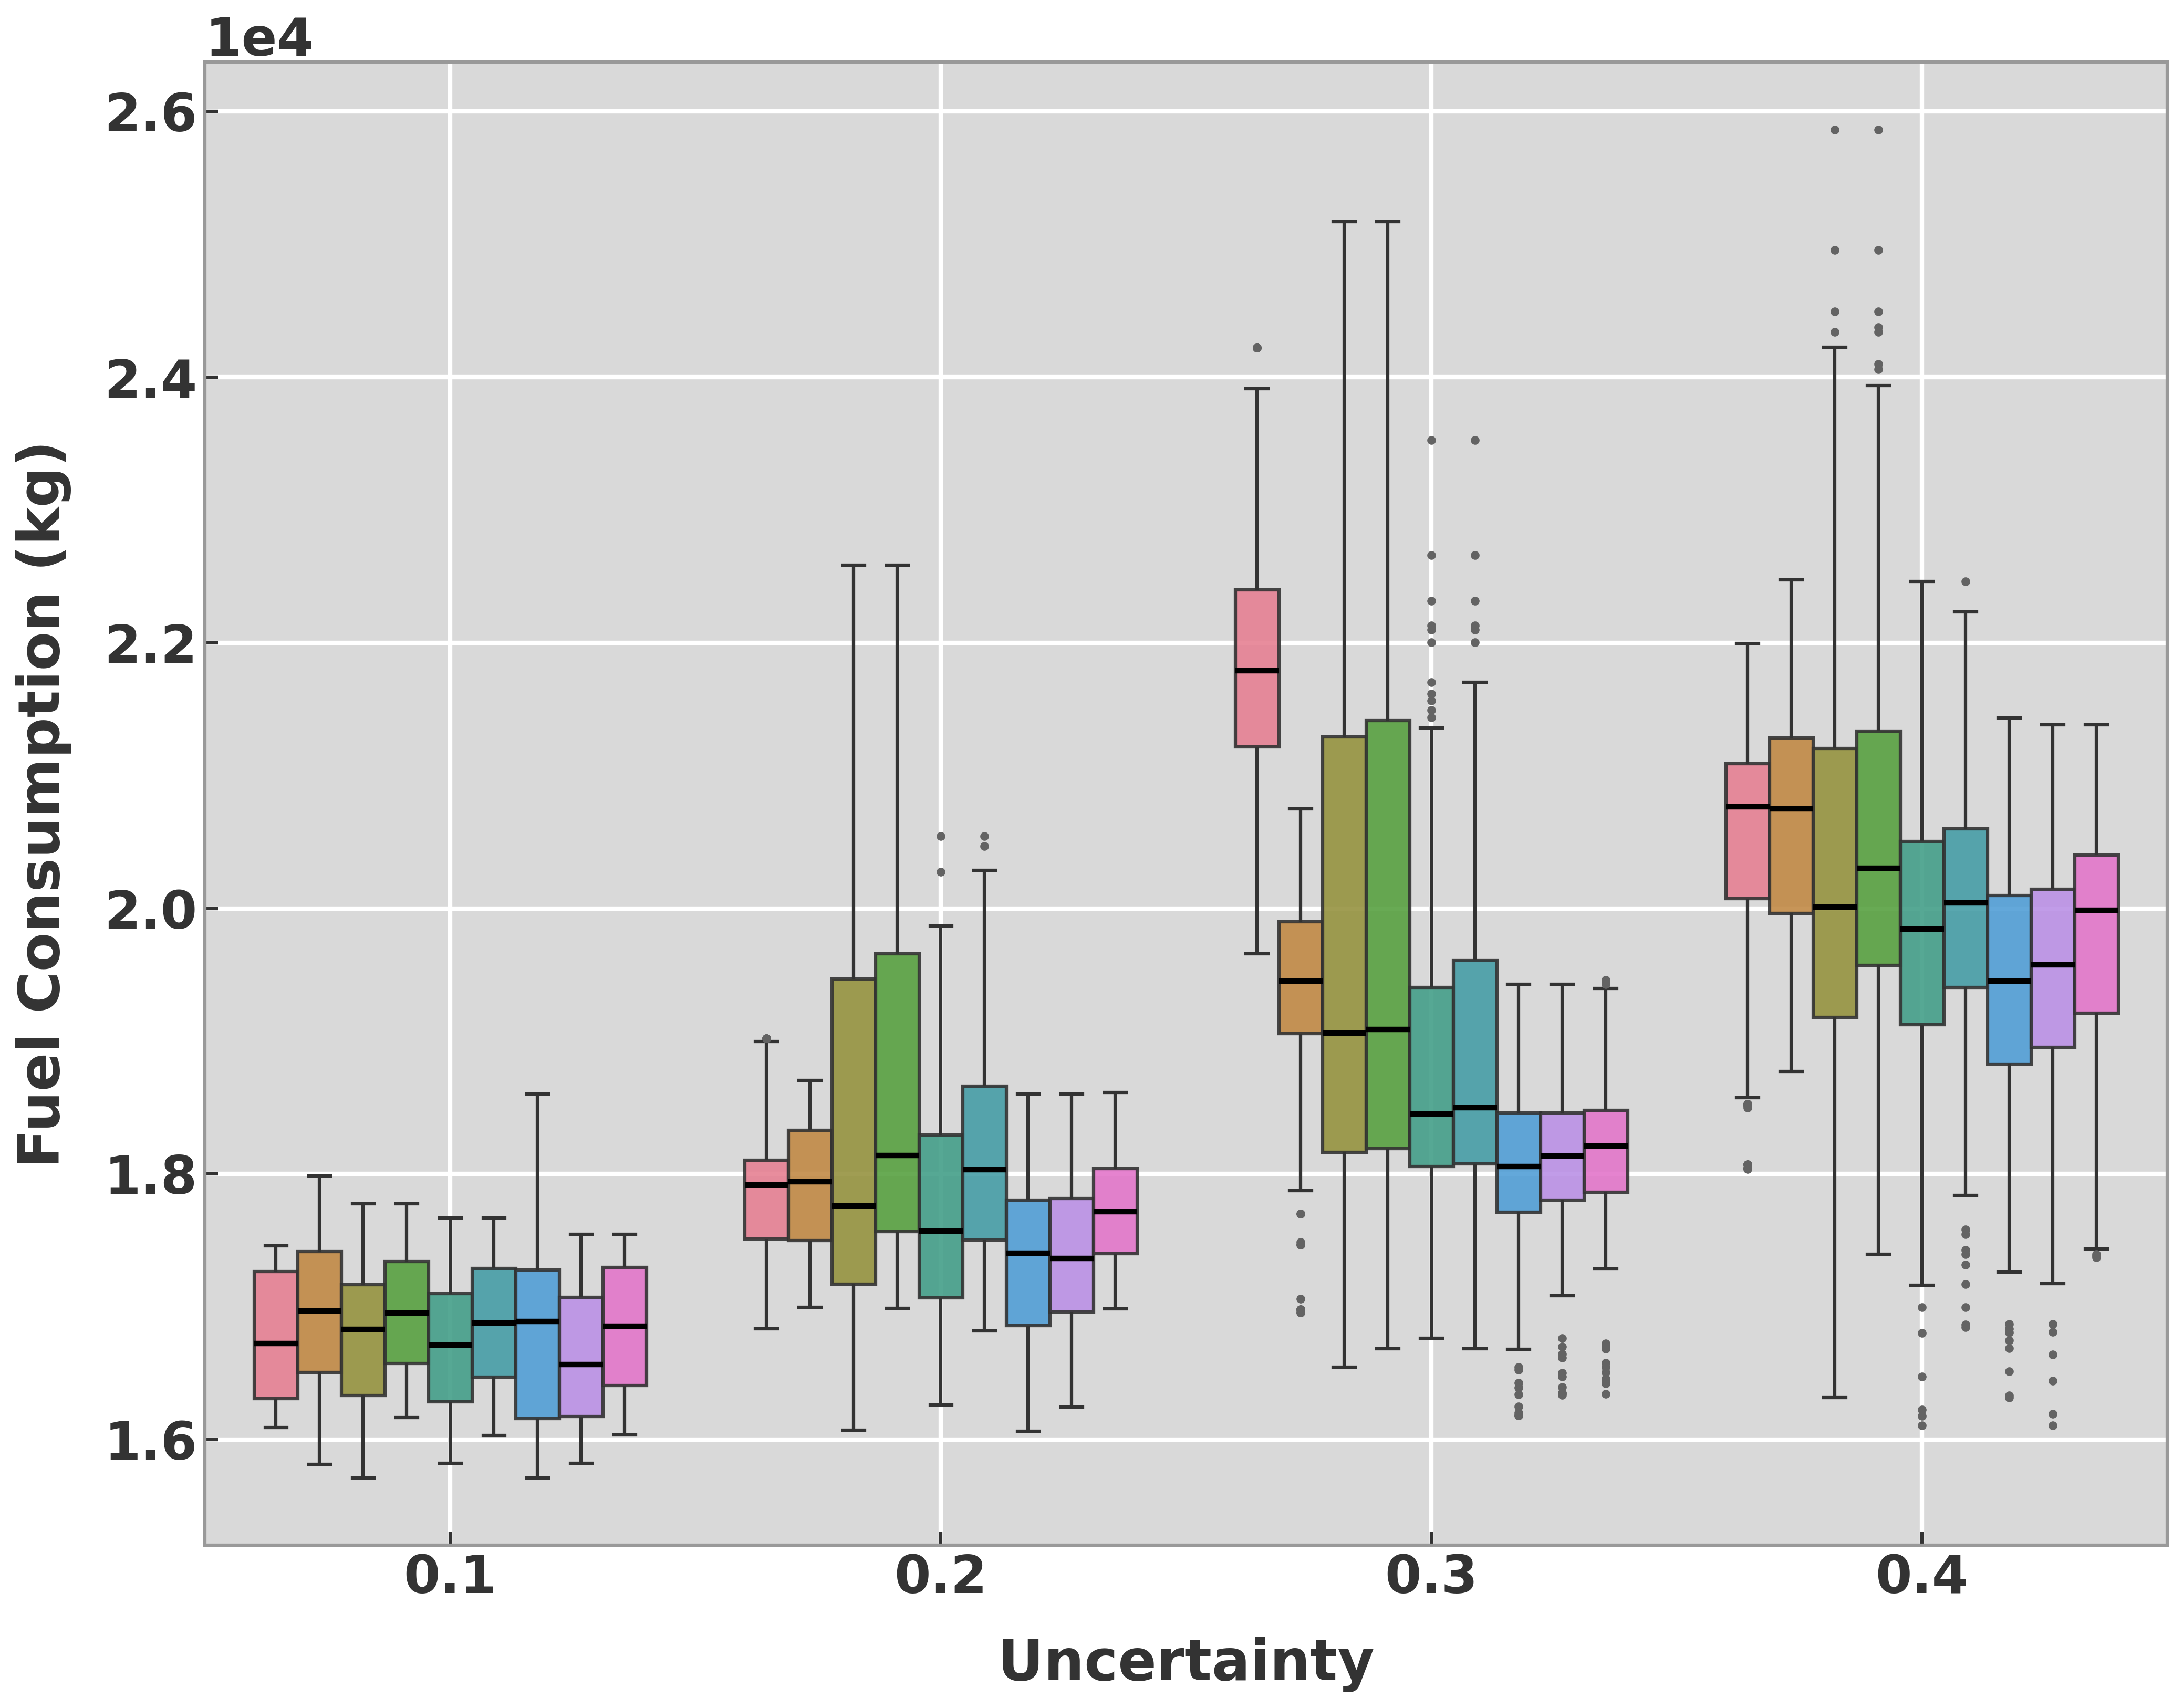
\includegraphics[width=0.45\textwidth]{figures/Traffic_0.8/traffic_0.8_fuel_consumption.png}
    }
    \hfill
    \subfloat[Traffic density = 0.9\label{fig:fc_b}]{
        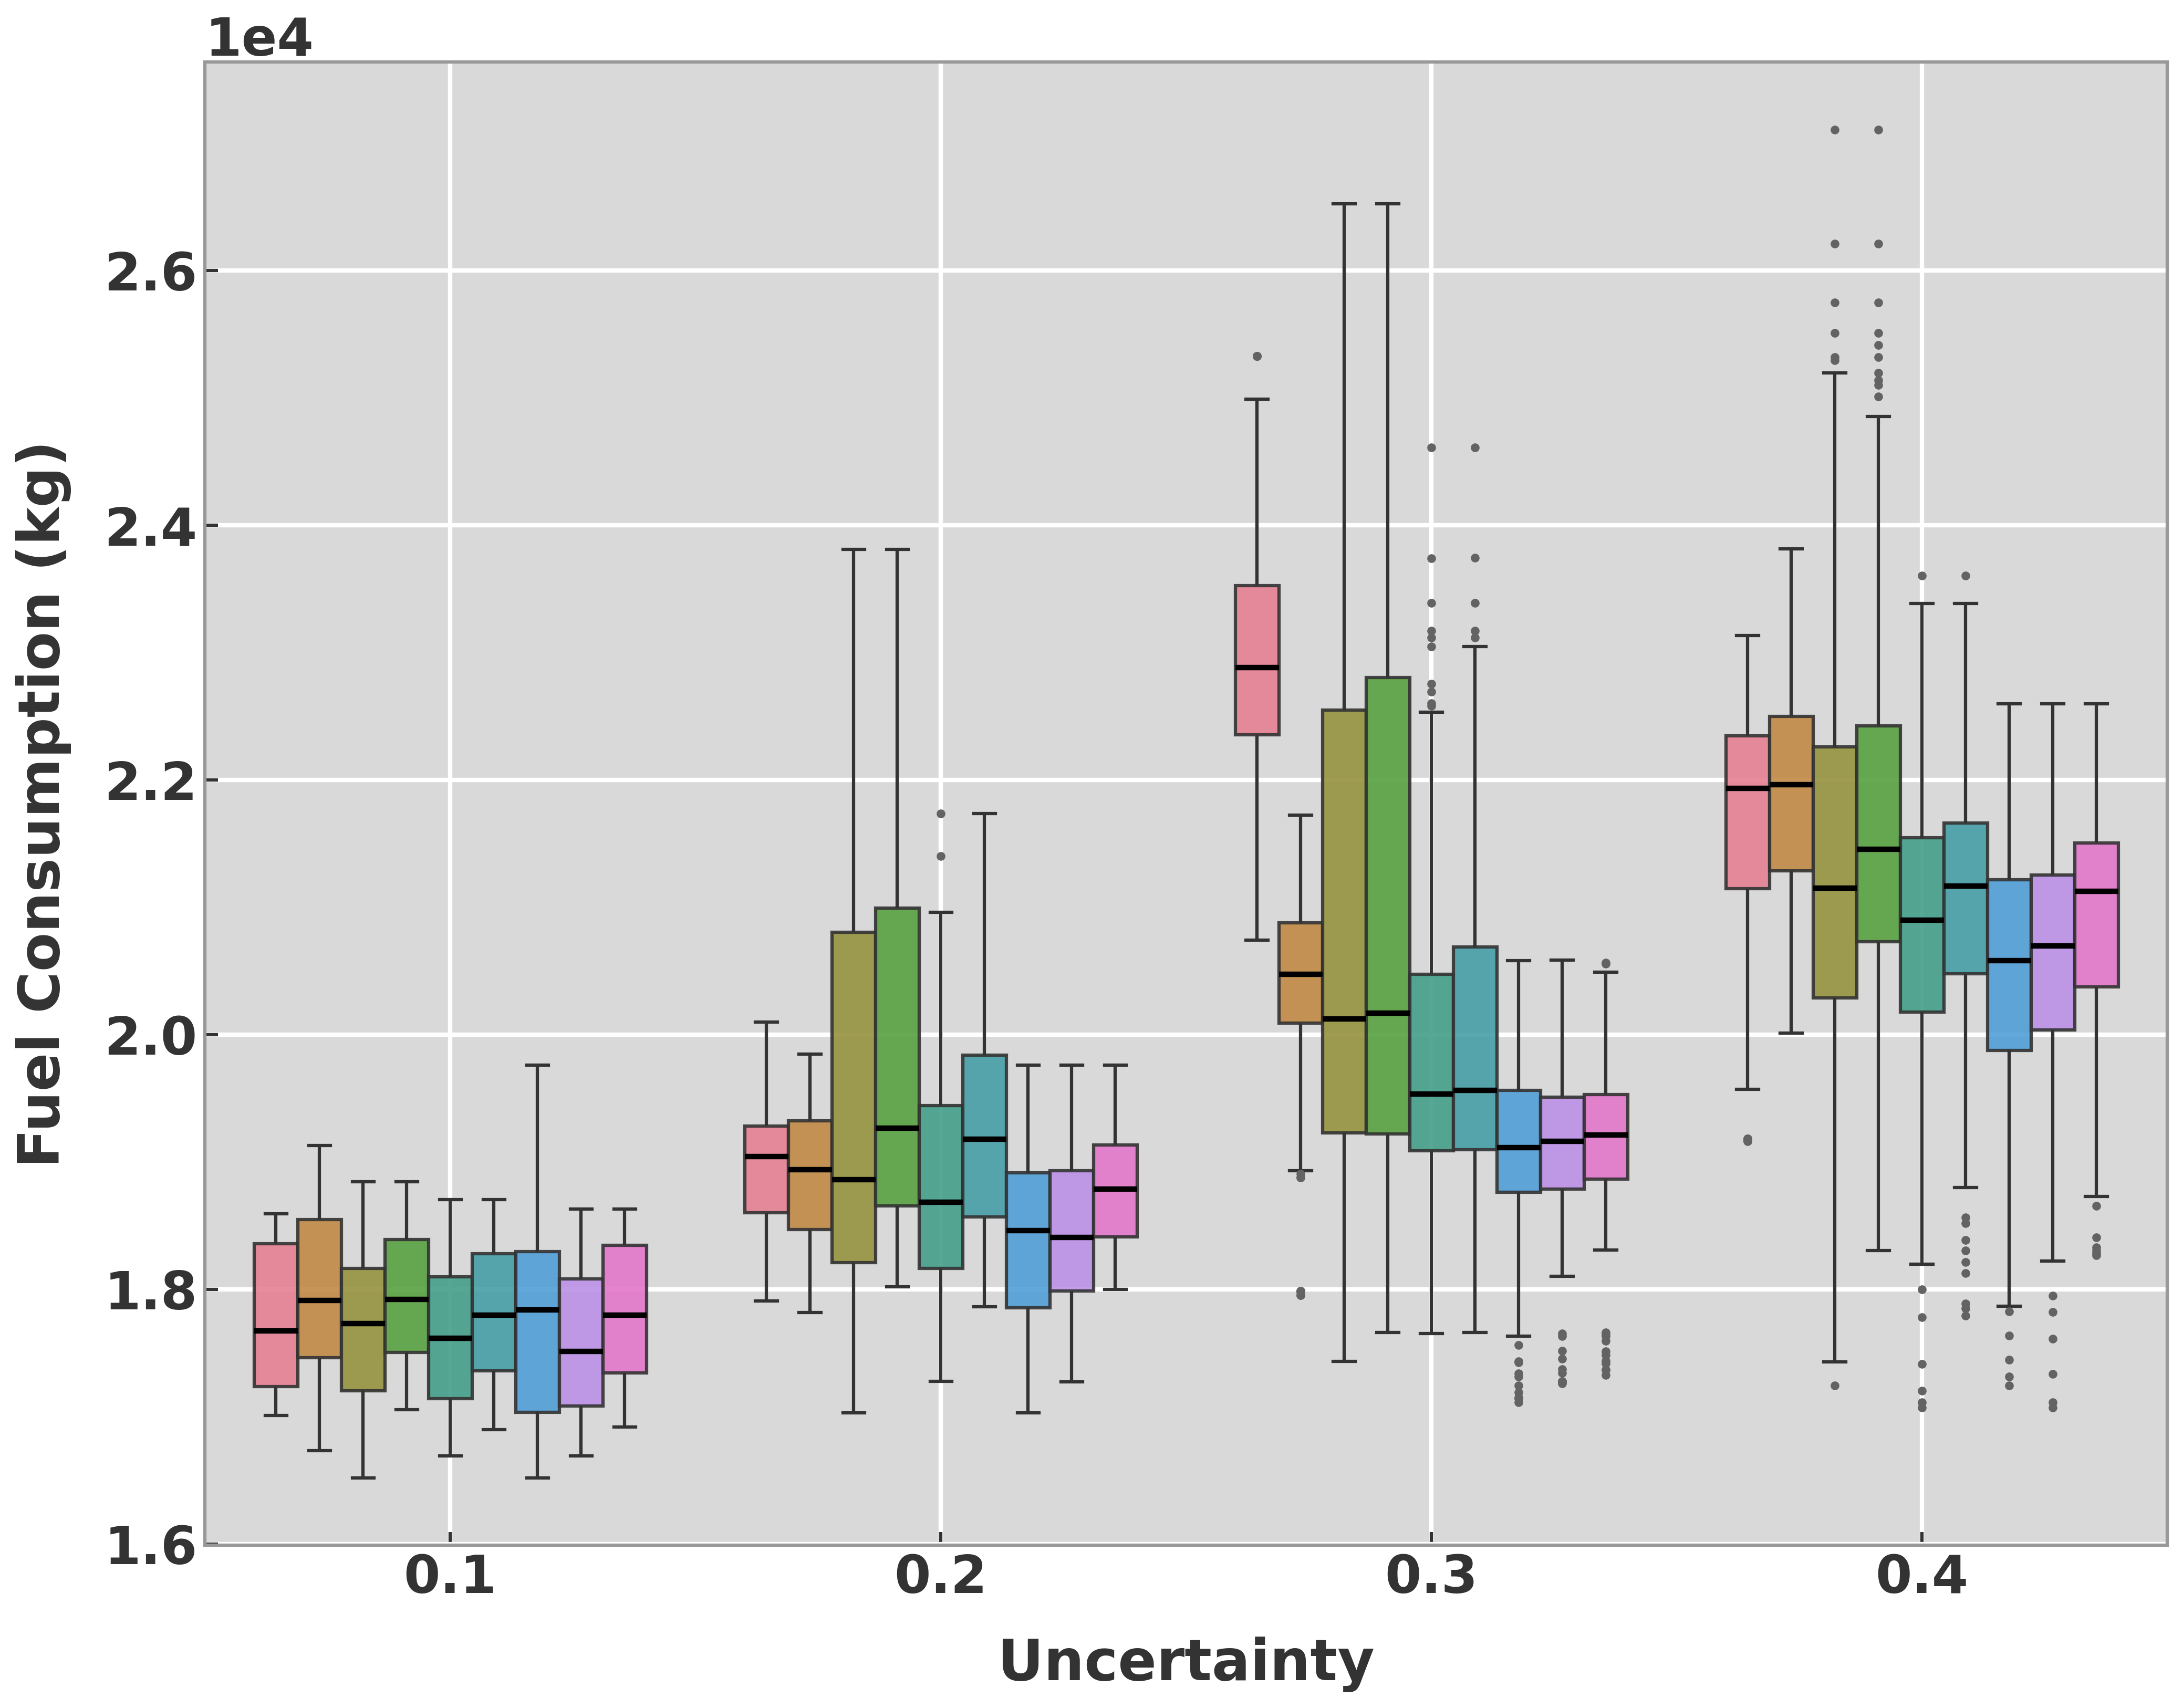
\includegraphics[width=0.45\textwidth]{figures/Traffic_0.9/traffic_0.9_fuel_consumption.png}
    }
    
    \subfloat[Traffic density = 1.0\label{fig:fc_c}]{
        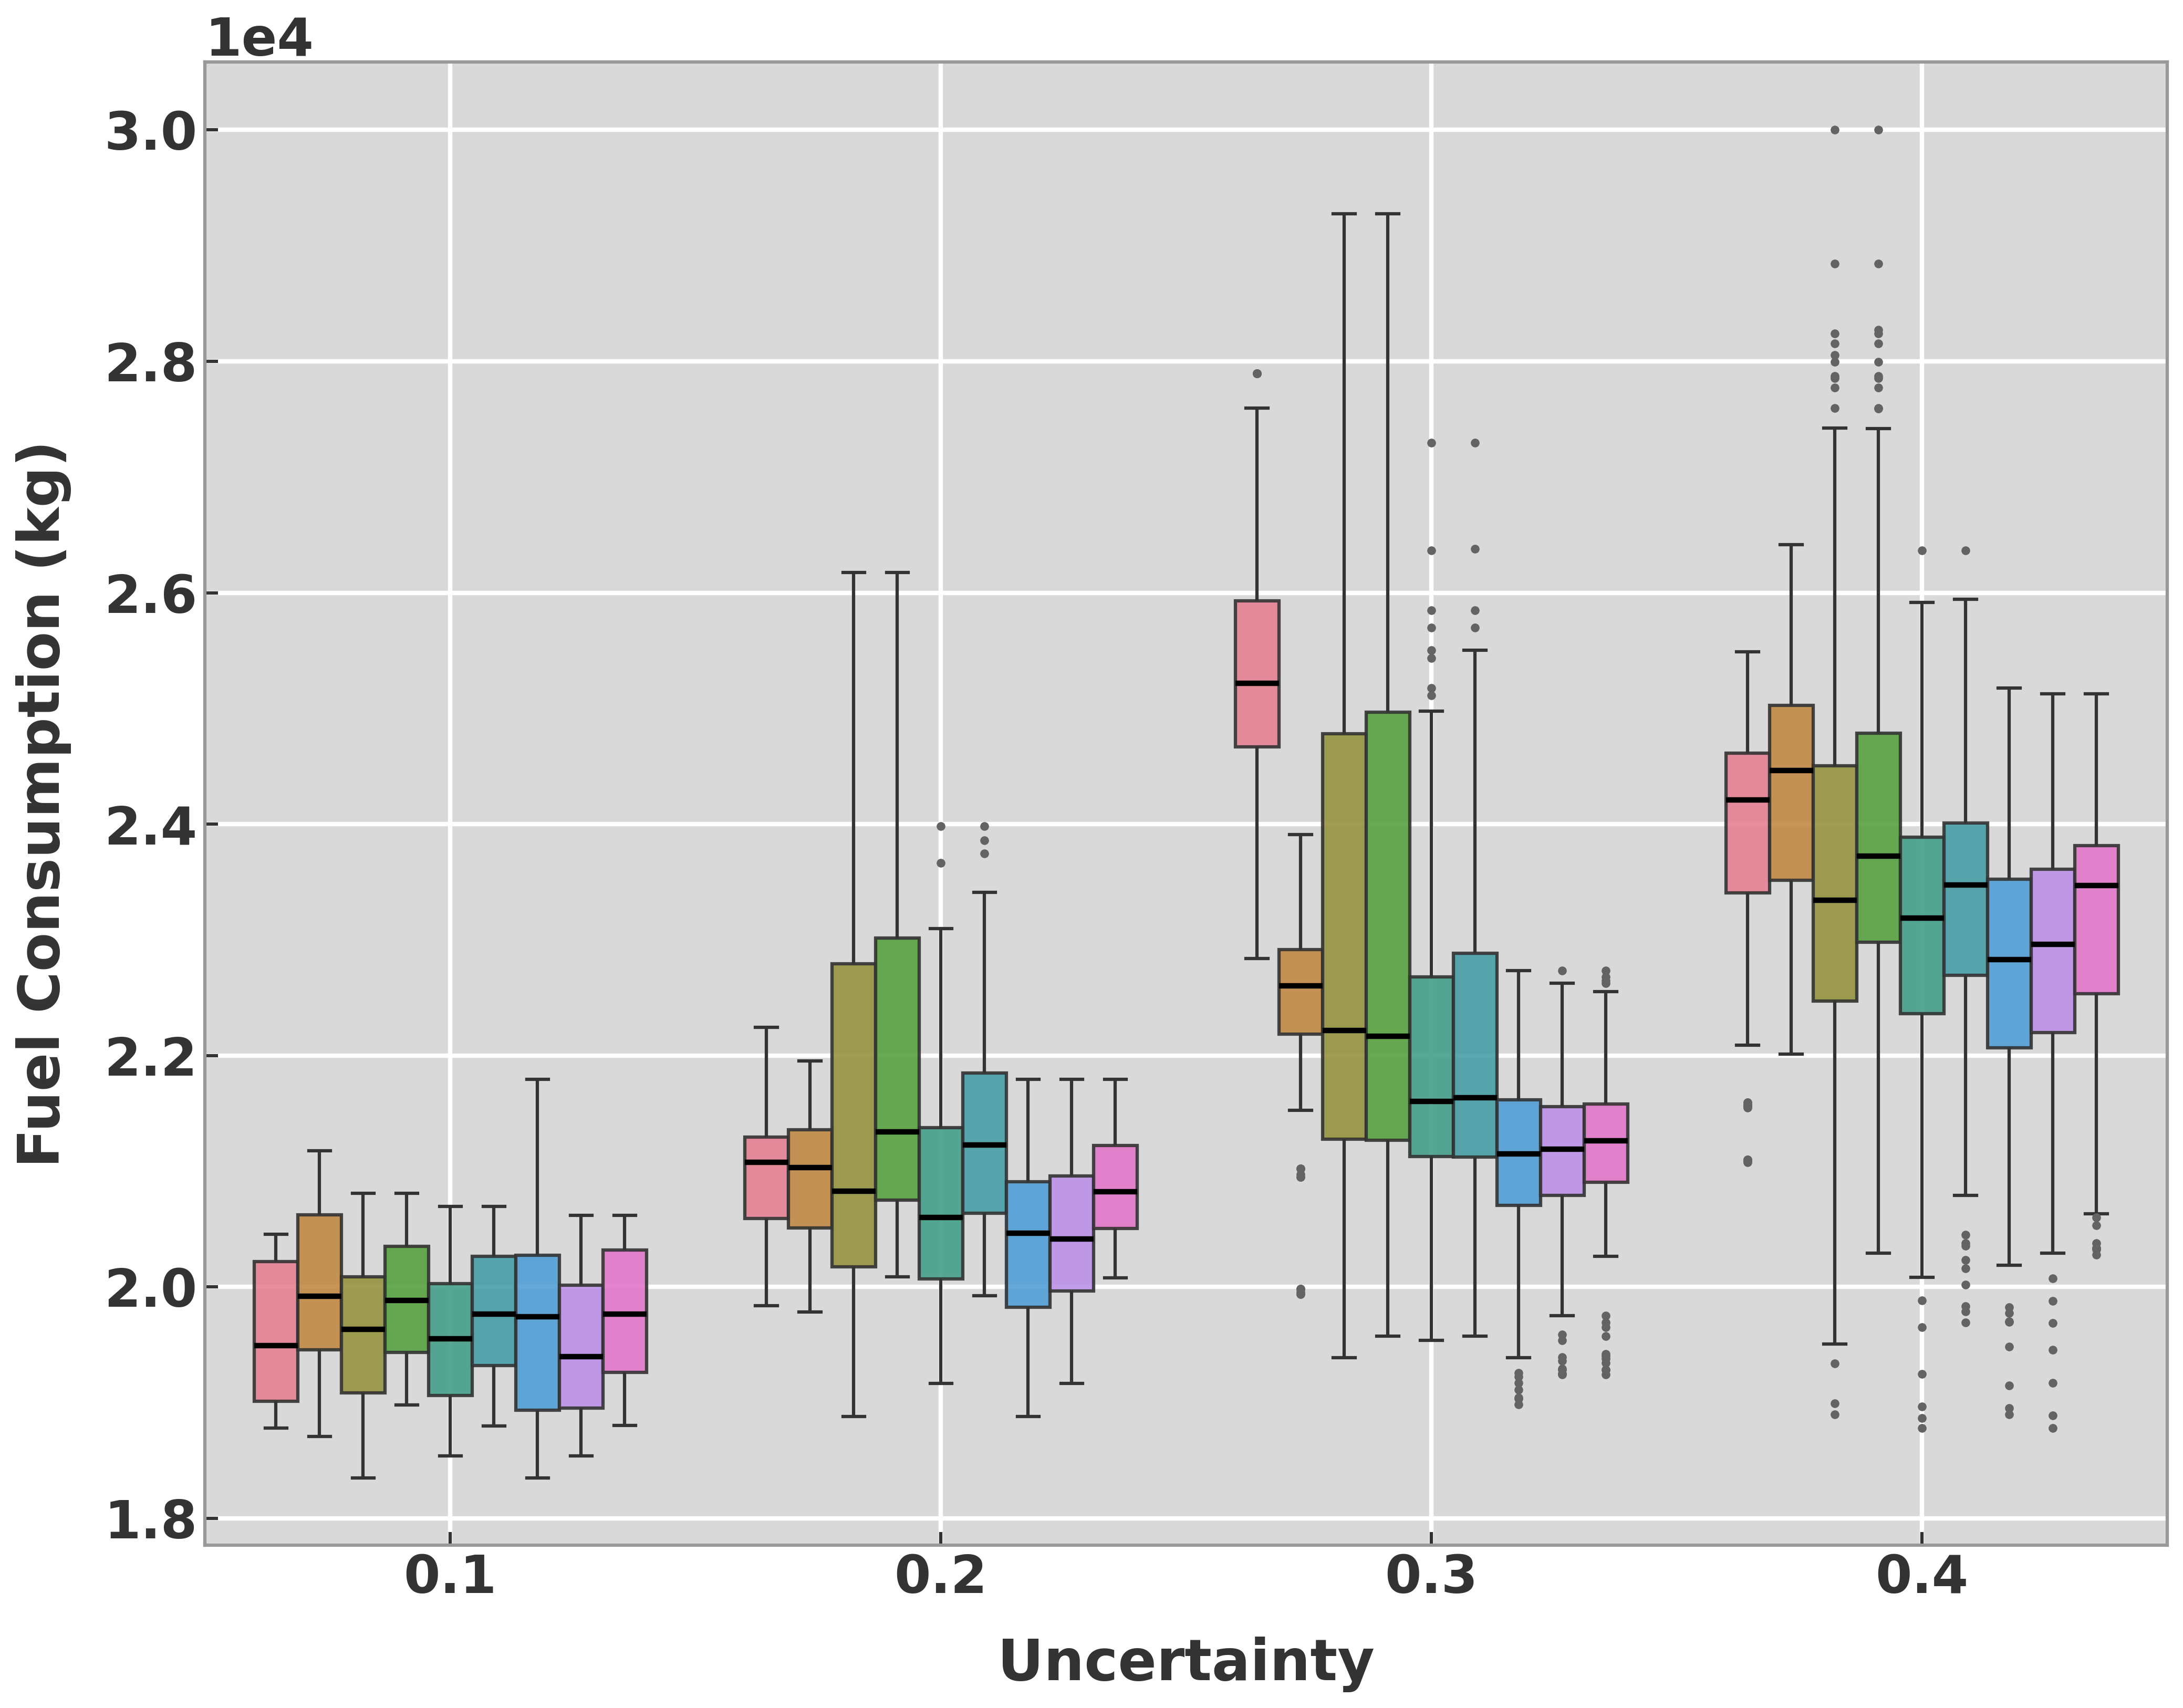
\includegraphics[width=0.45\textwidth]{figures/Traffic_1.0/traffic_1.0_fuel_consumption.png}
    }
    \hfill
    \subfloat[Traffic density = 1.1\label{fig:fc_d}]{
        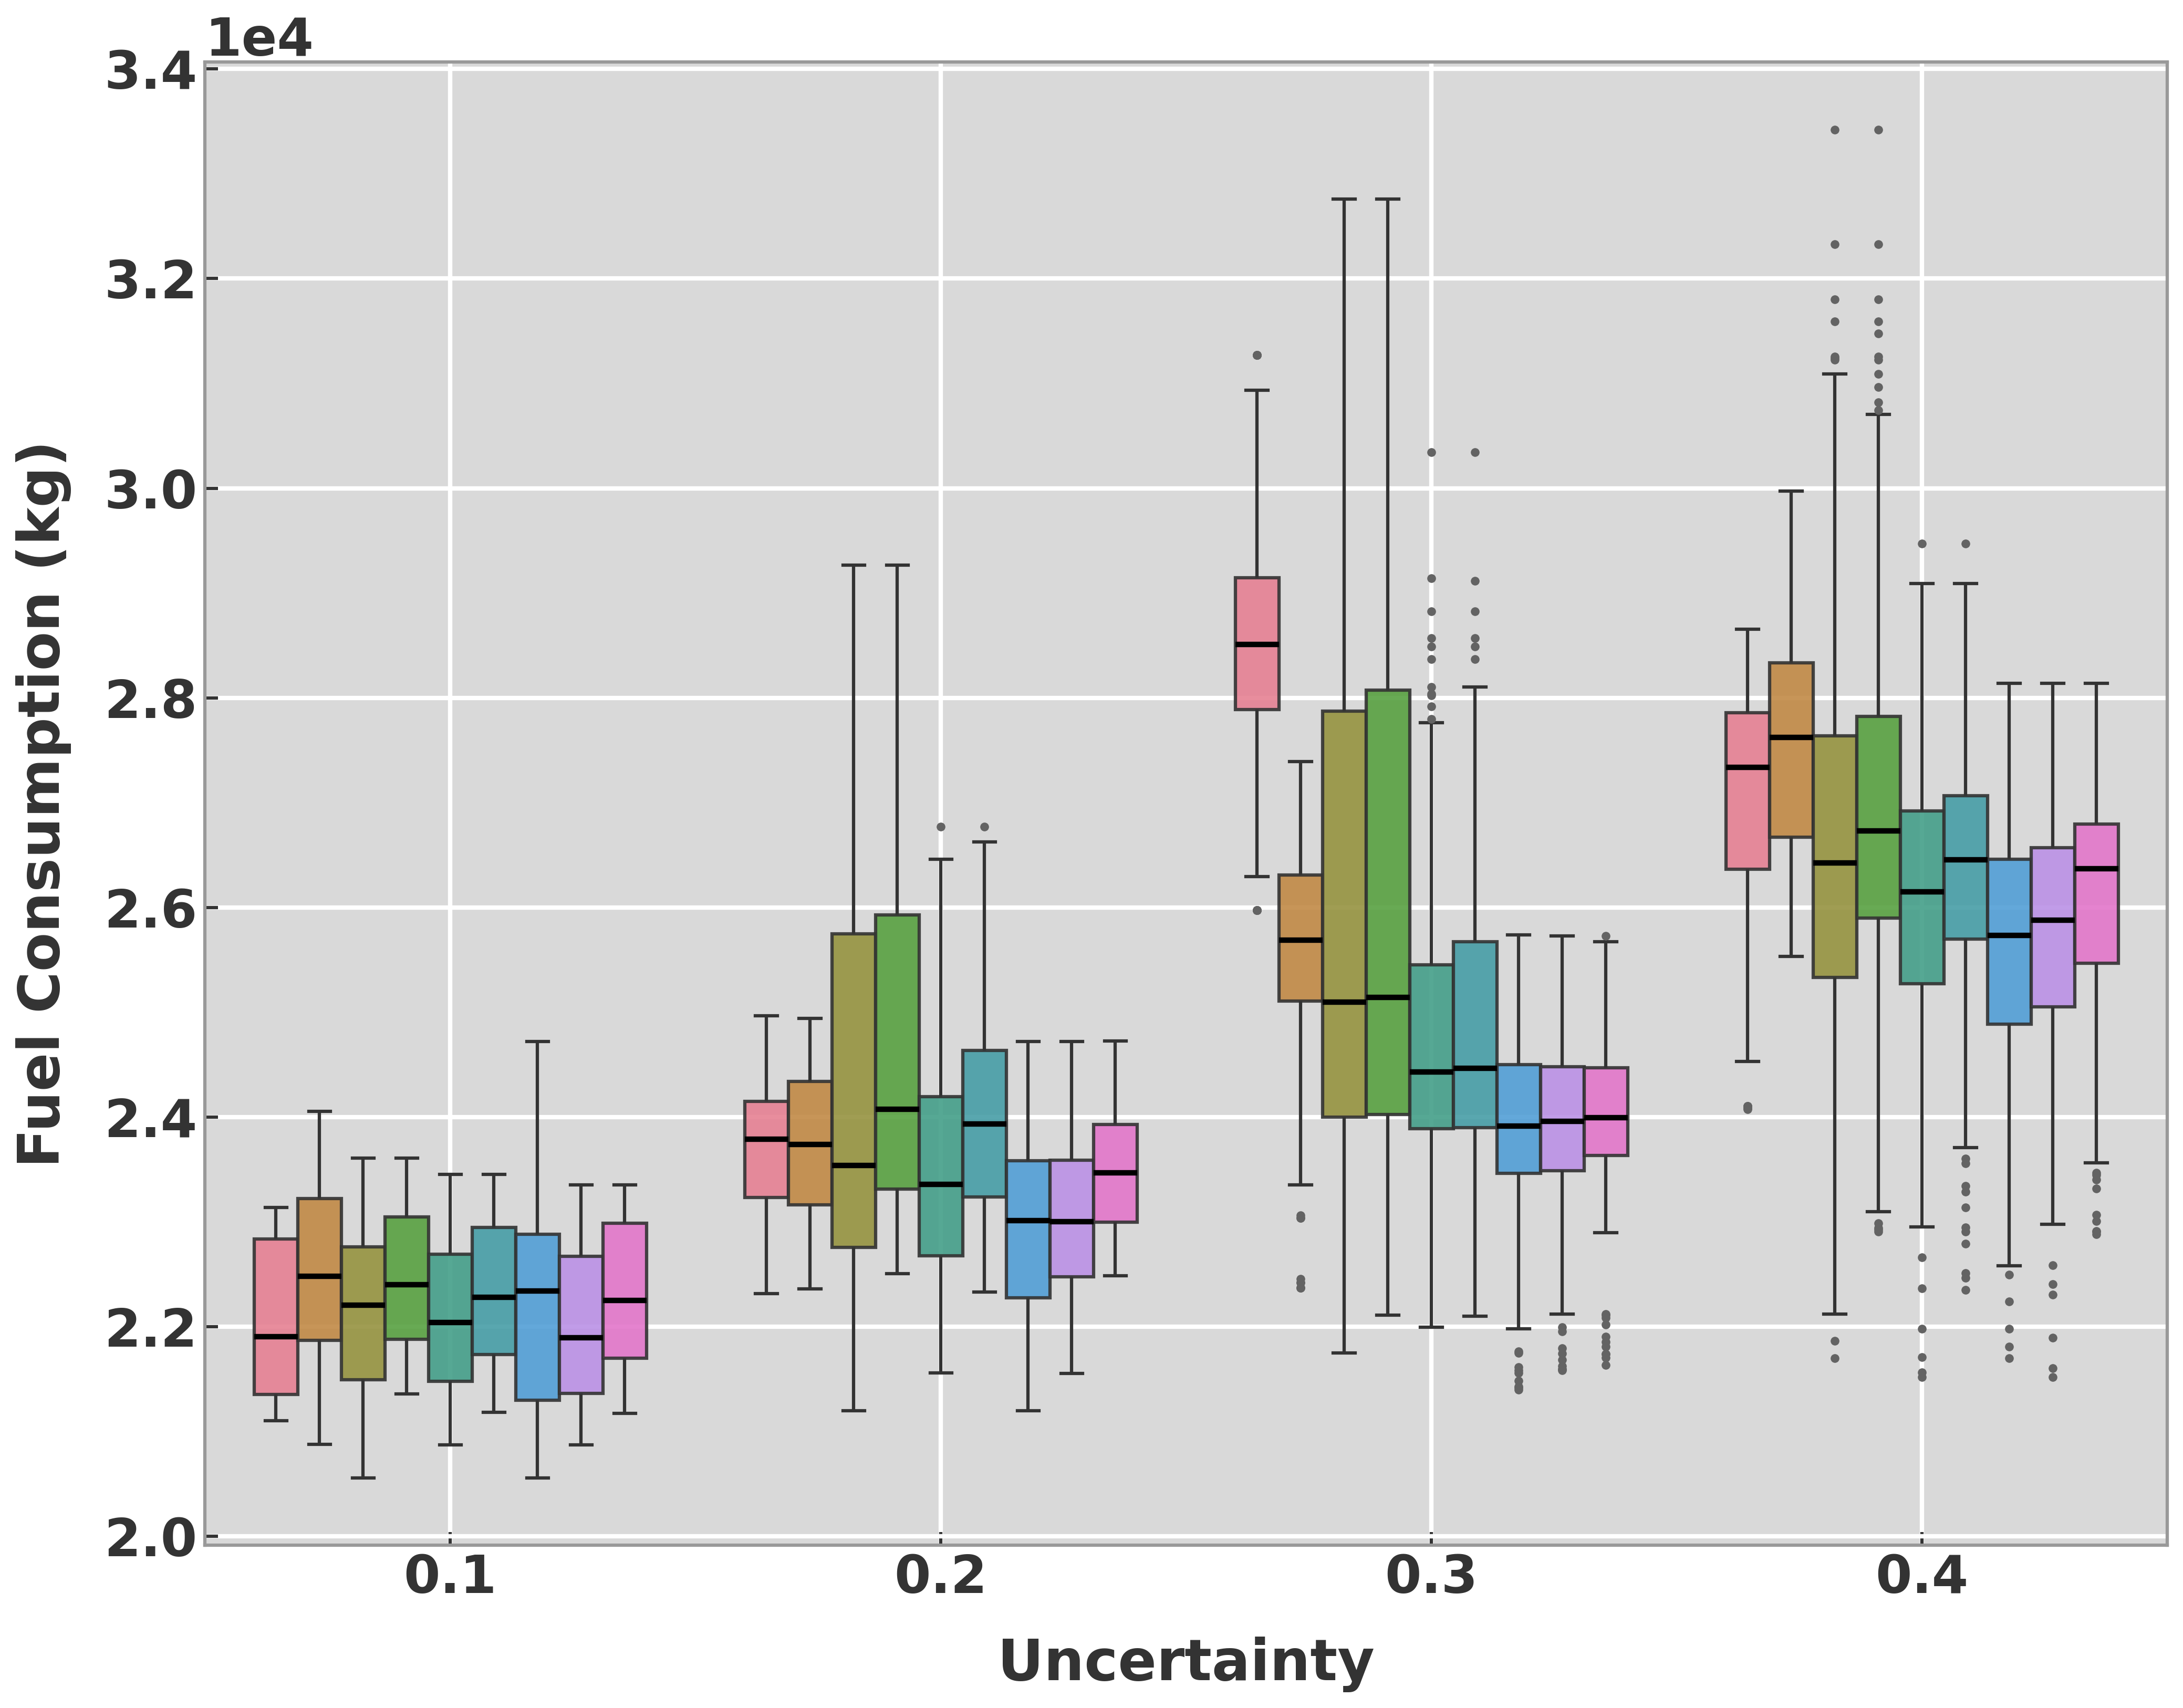
\includegraphics[width=0.45\textwidth]{figures/Traffic_1.1/traffic_1.1_fuel_consumption.png}
    }
    
    \centering
    \subfloat[Traffic density = 1.2\label{fig:fc_e}]{
        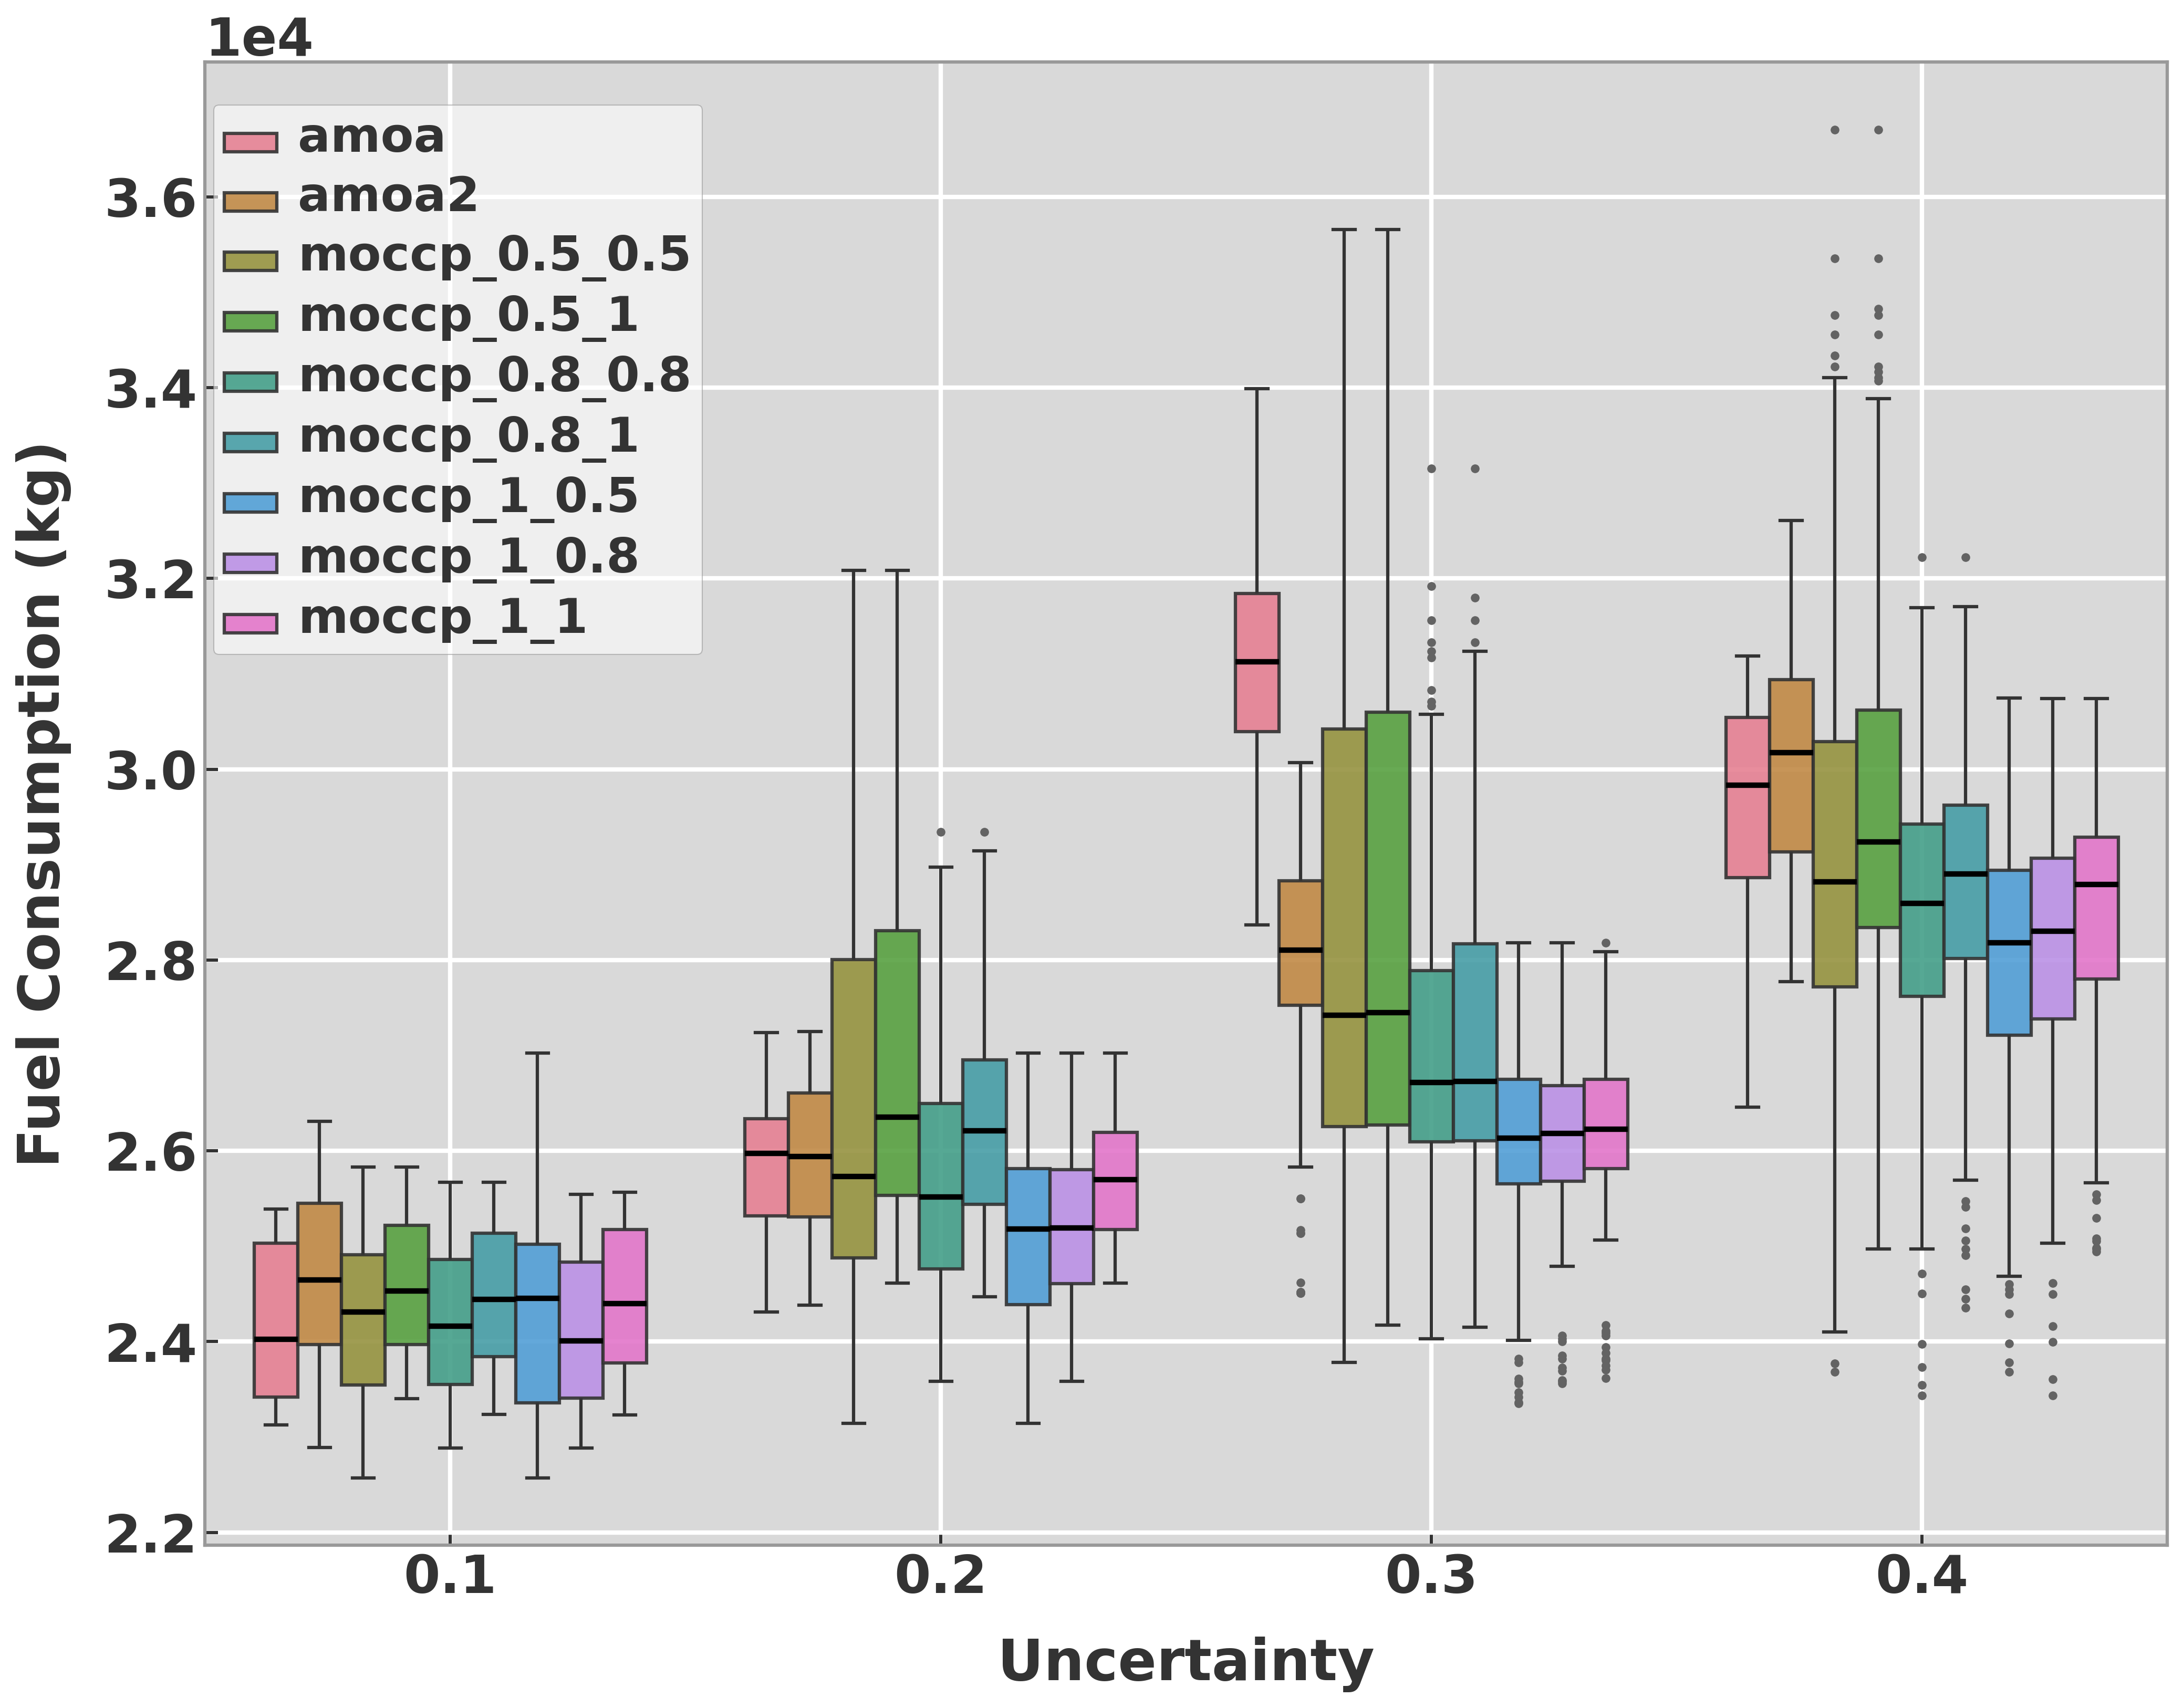
\includegraphics[width=0.45\textwidth]{figures/Traffic_1.2/traffic_1.2_fuel_consumption.png}
    }
    
    \caption{Fuel consumption under different traffic densities. In each sub figure, each group of nine bars has the same level of uncertainties.}
    \label{fig:fc}
\end{figure}



% \begin{figure}[htp]
%     \centering
%     \subfigure(a){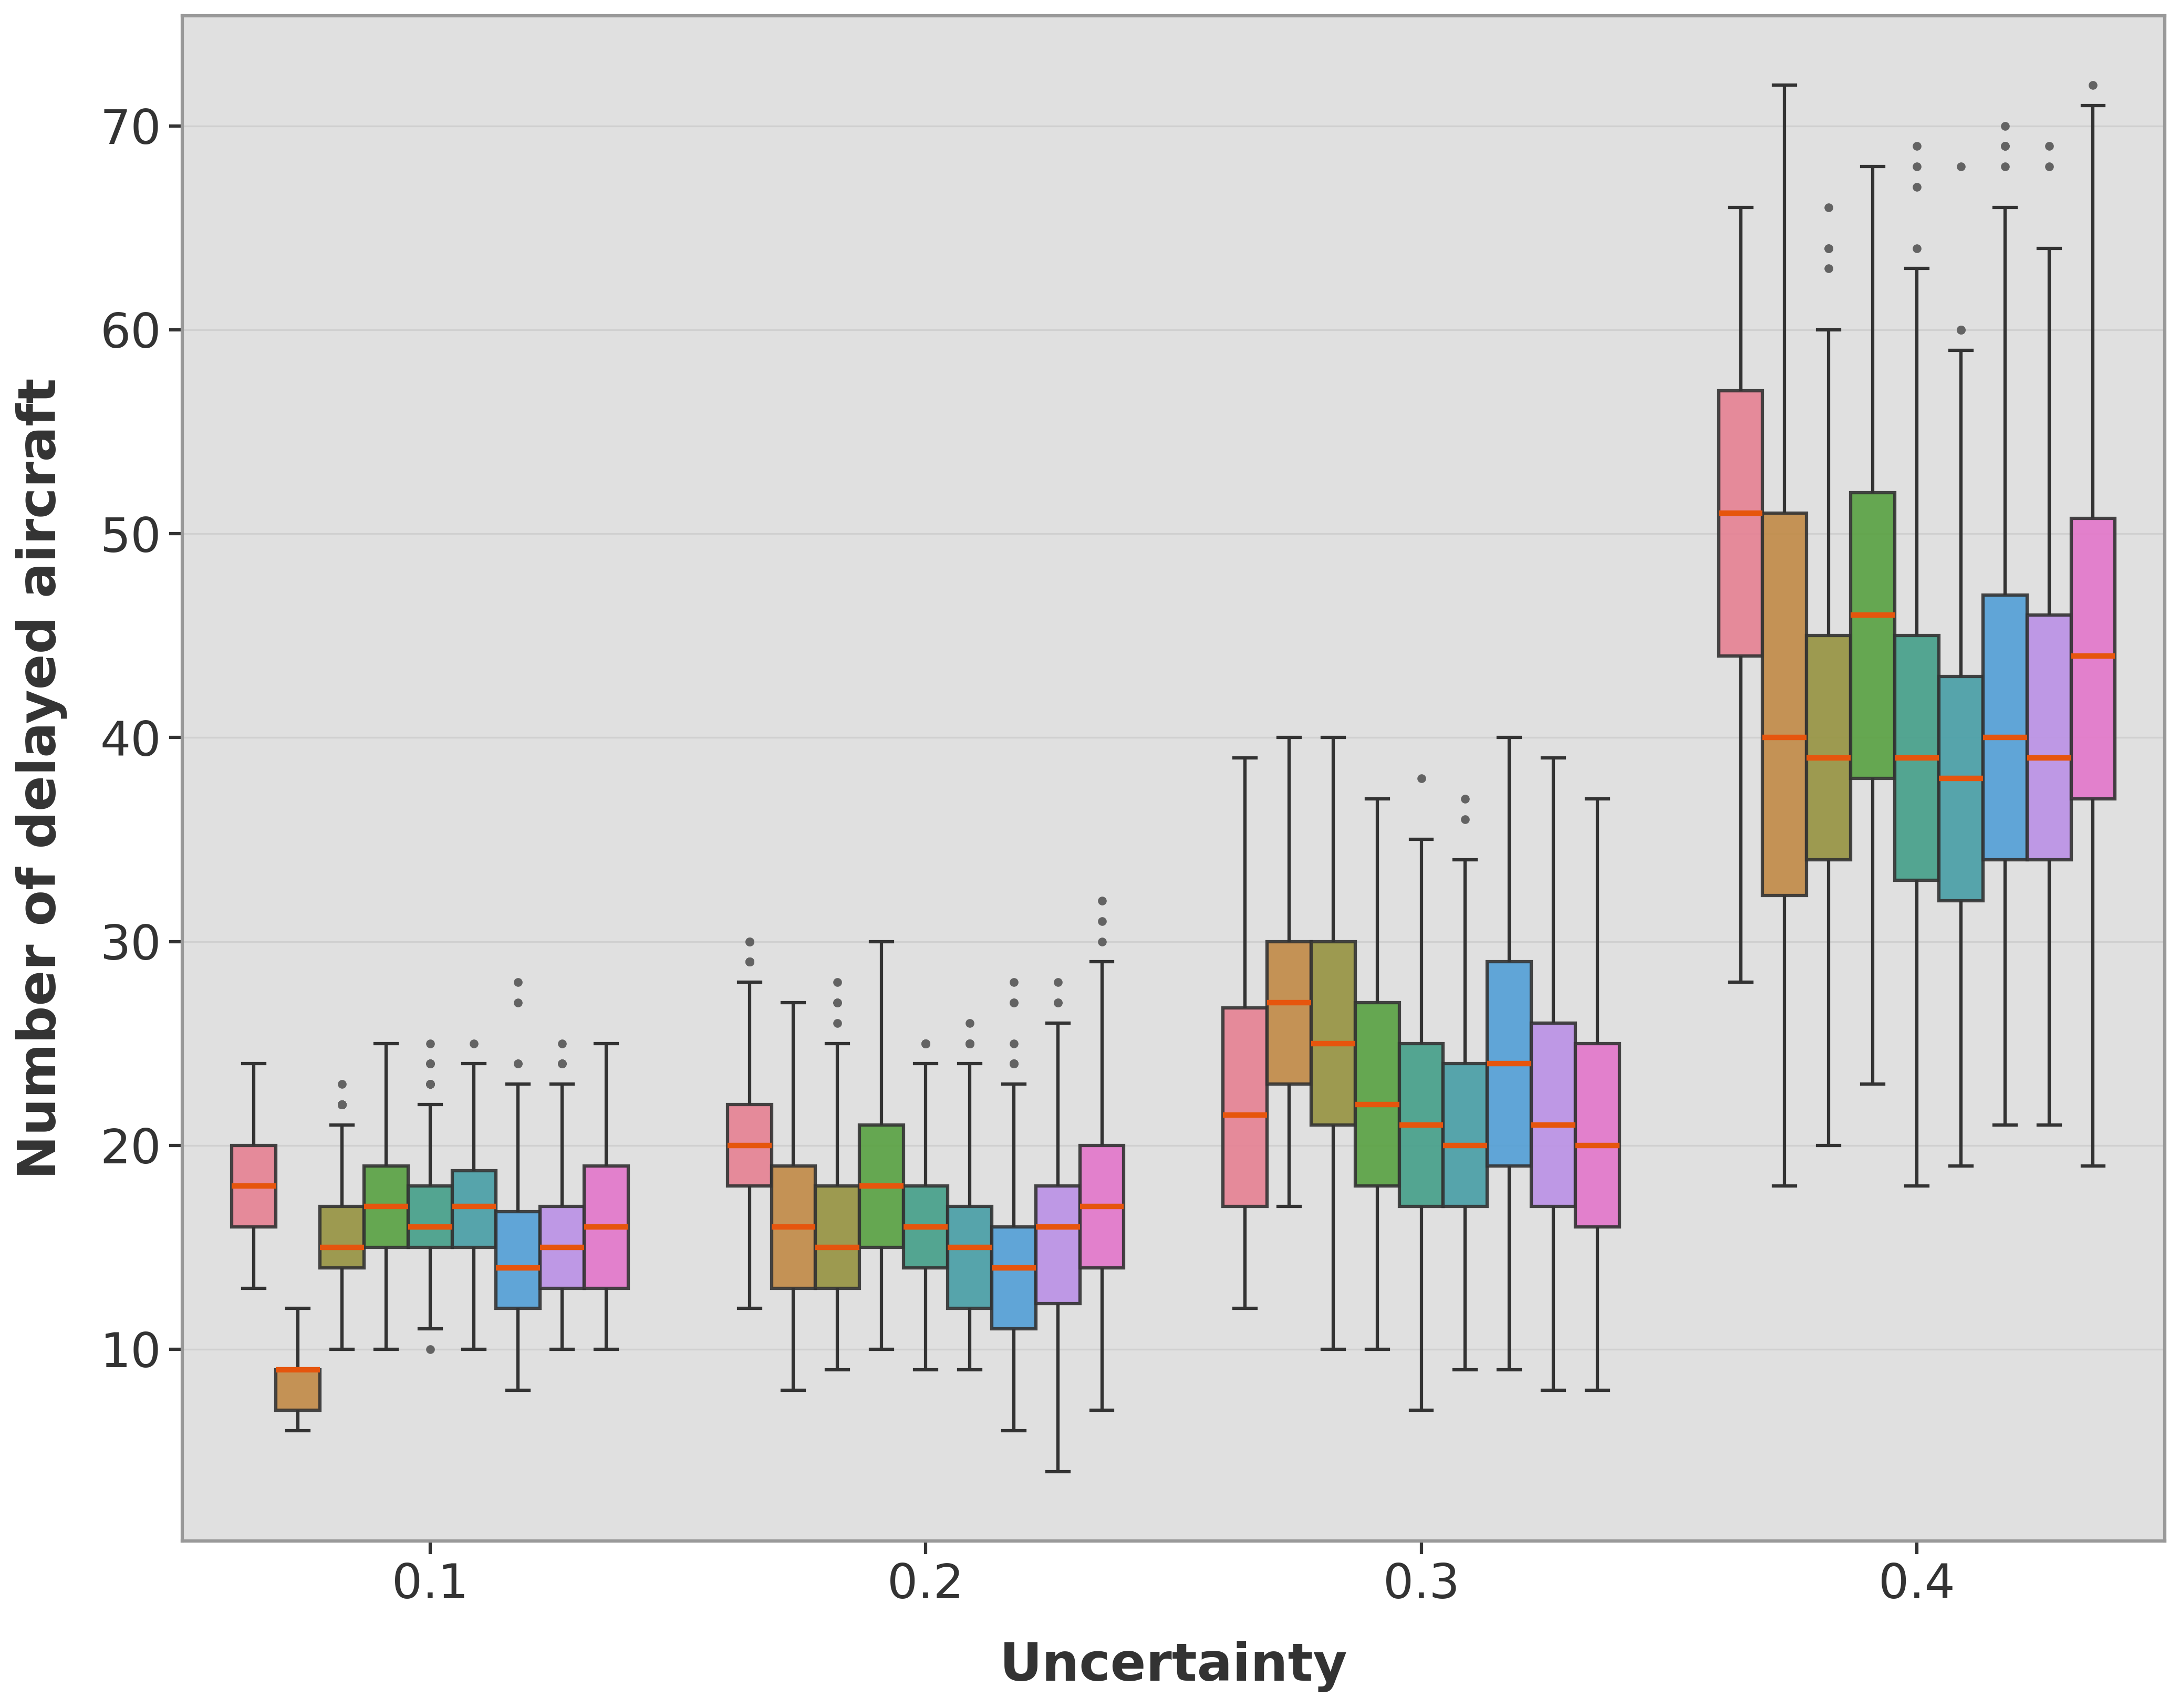
\includegraphics[width=0.45\textwidth]{figures/Traffic_0.8/traffic_0.8_delayed_30s_count.png}} 
%     \subfigure(b){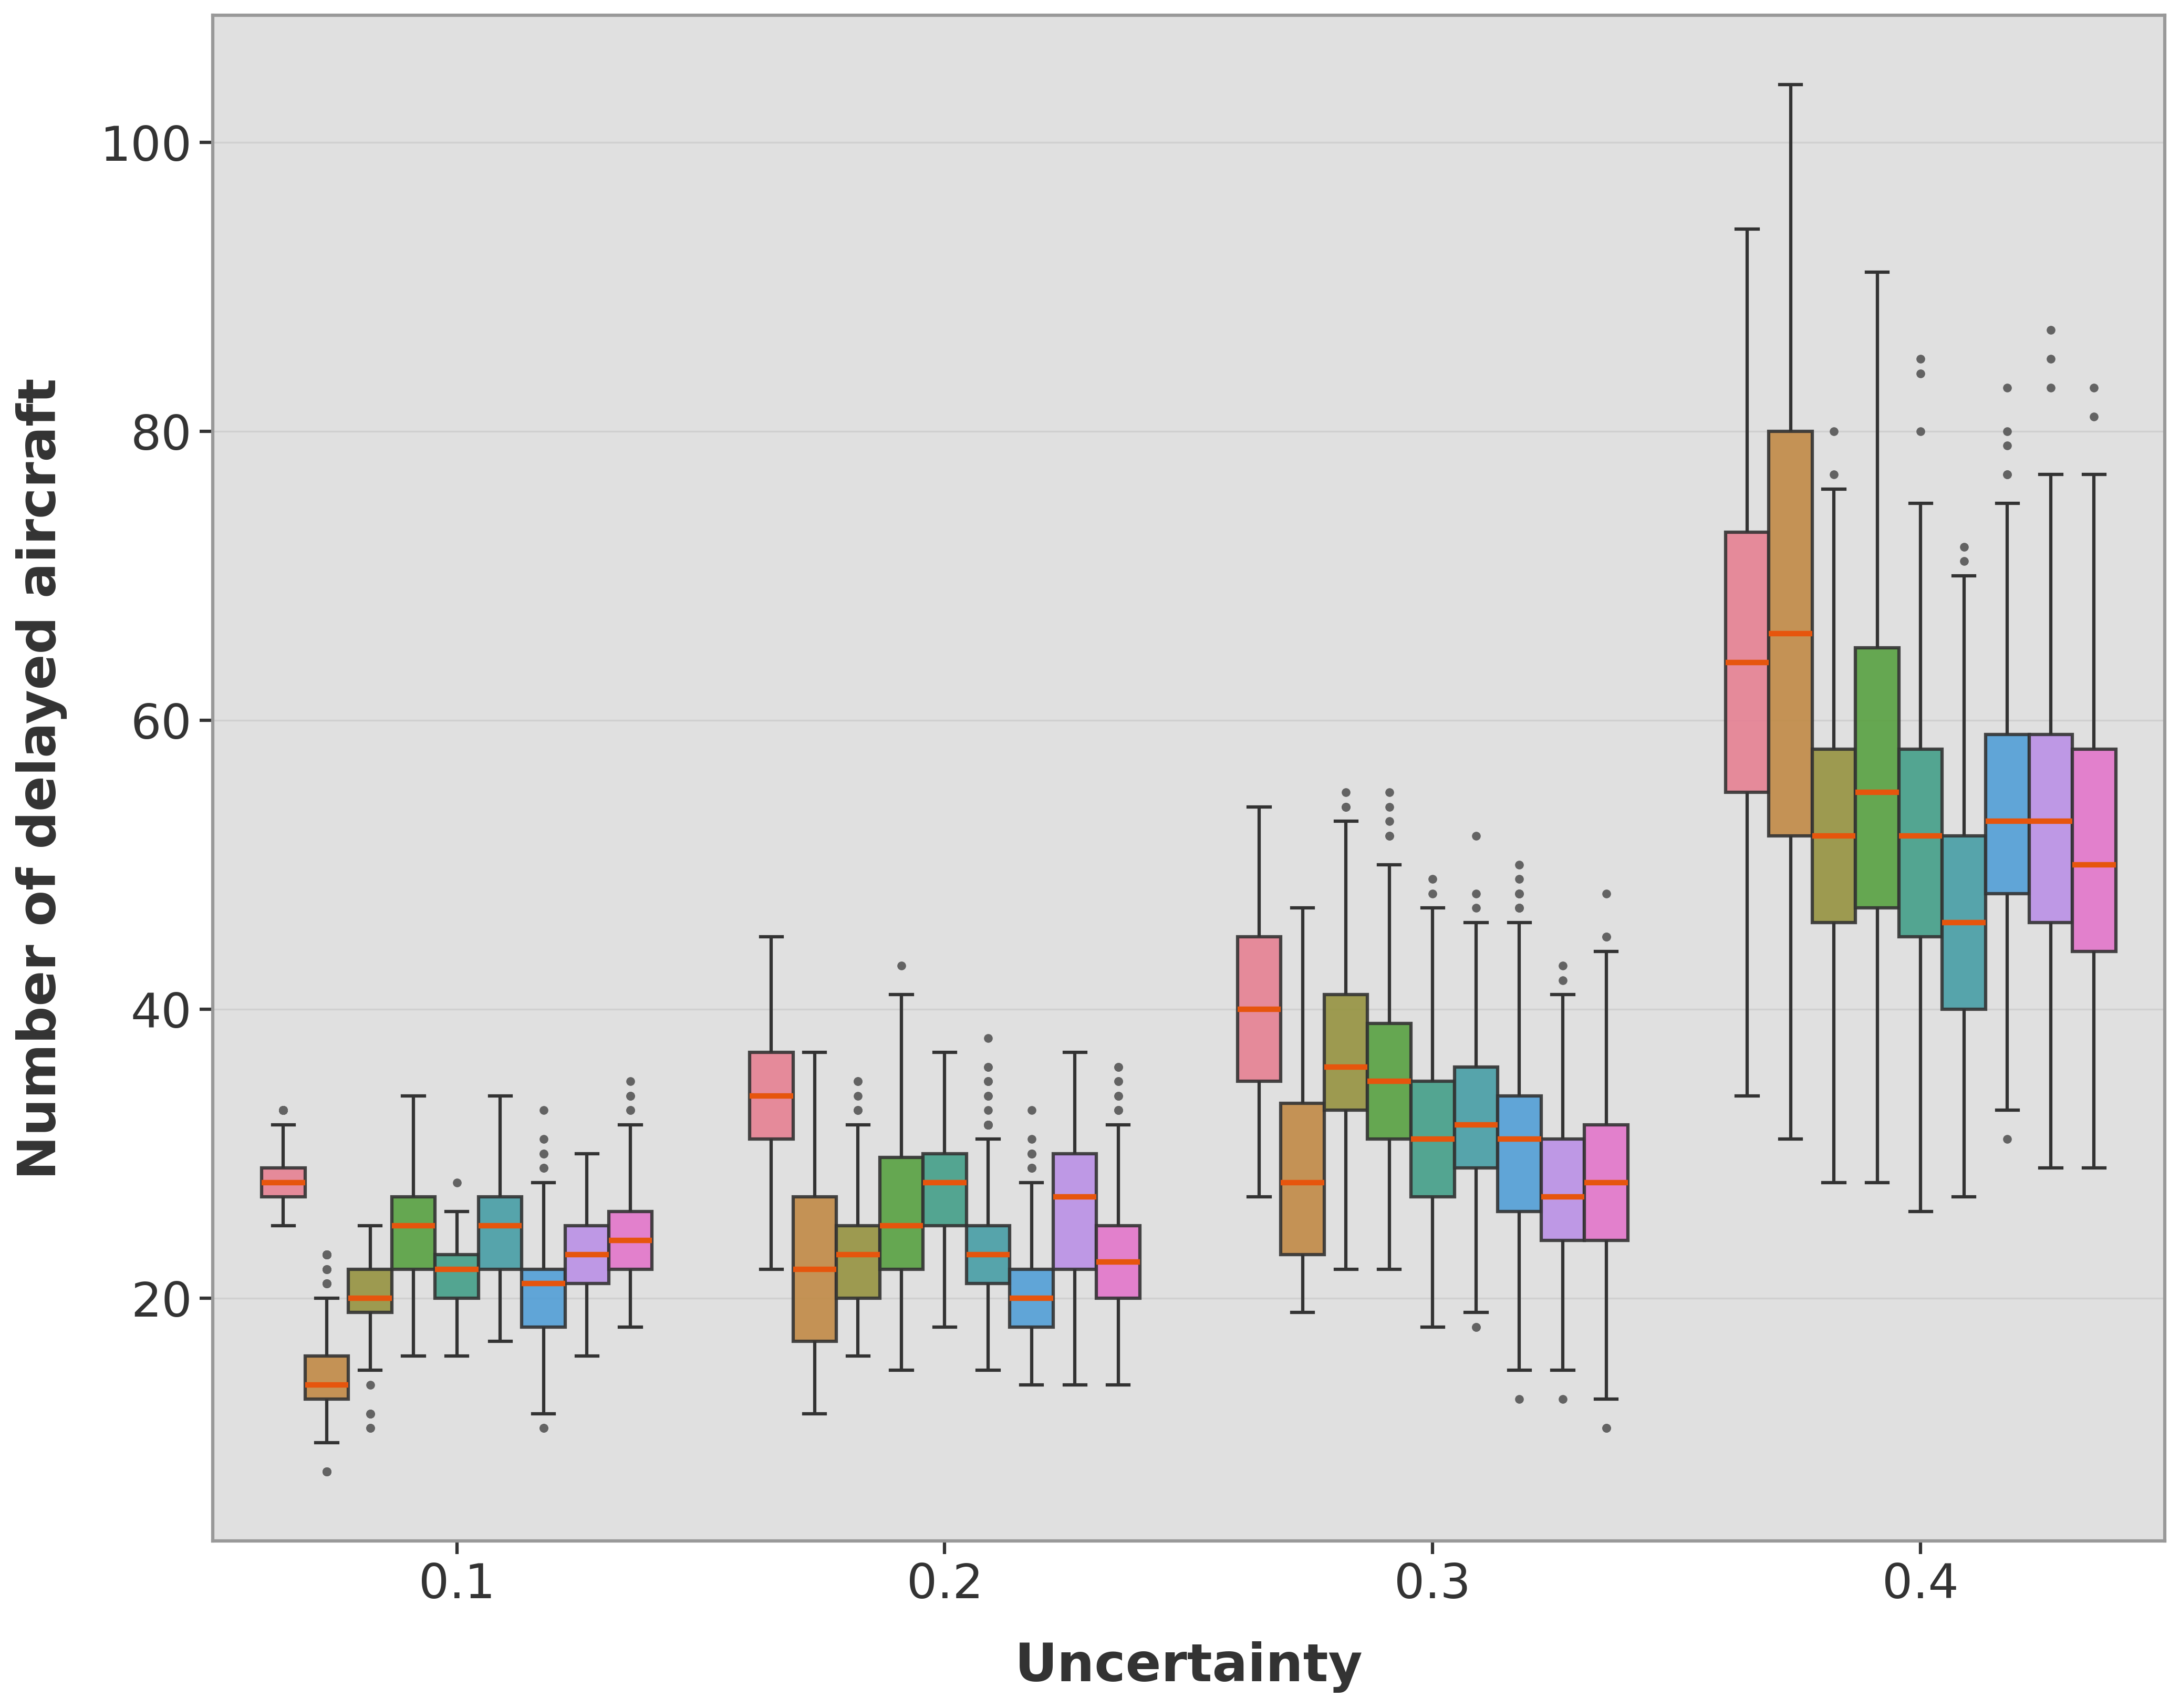
\includegraphics[width=0.45\textwidth]{figures/Traffic_0.9/traffic_0.9_delayed_30s_count.png}} 
%     \subfigure(c){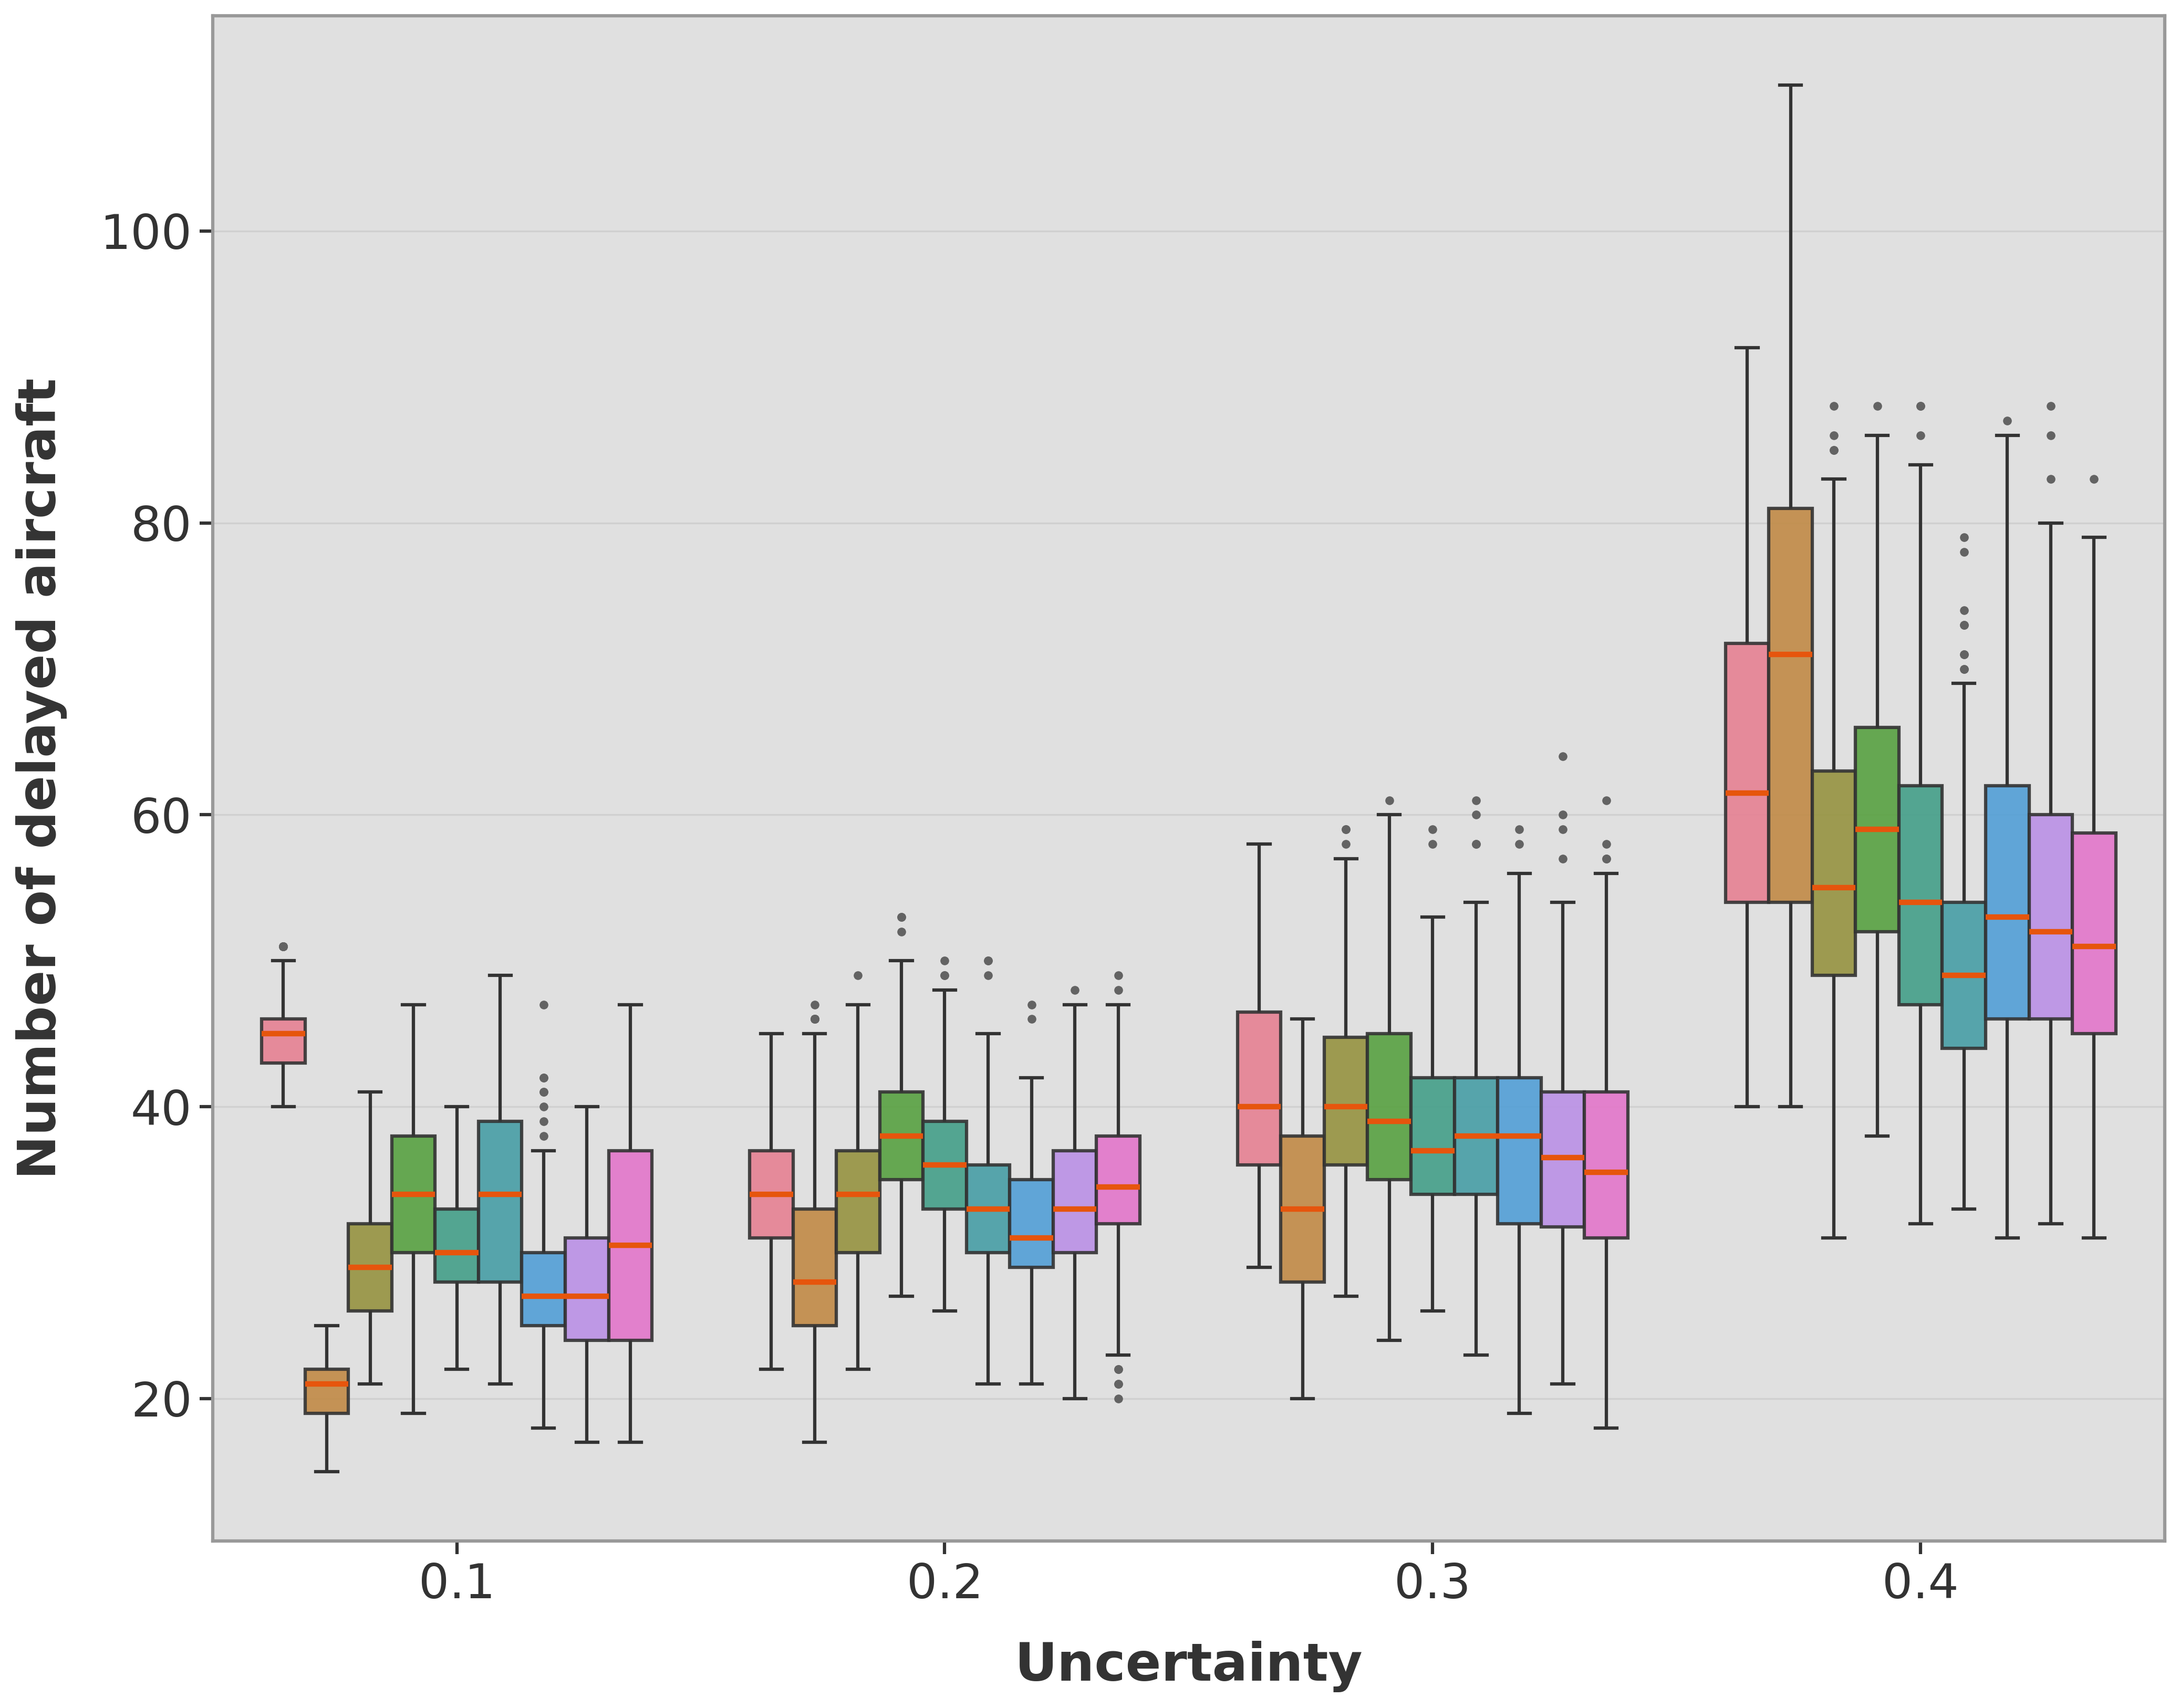
\includegraphics[width=0.45\textwidth]{figures/Traffic_1.0/traffic_1.0_delayed_30s_count.png}} 
%       \subfigure(d){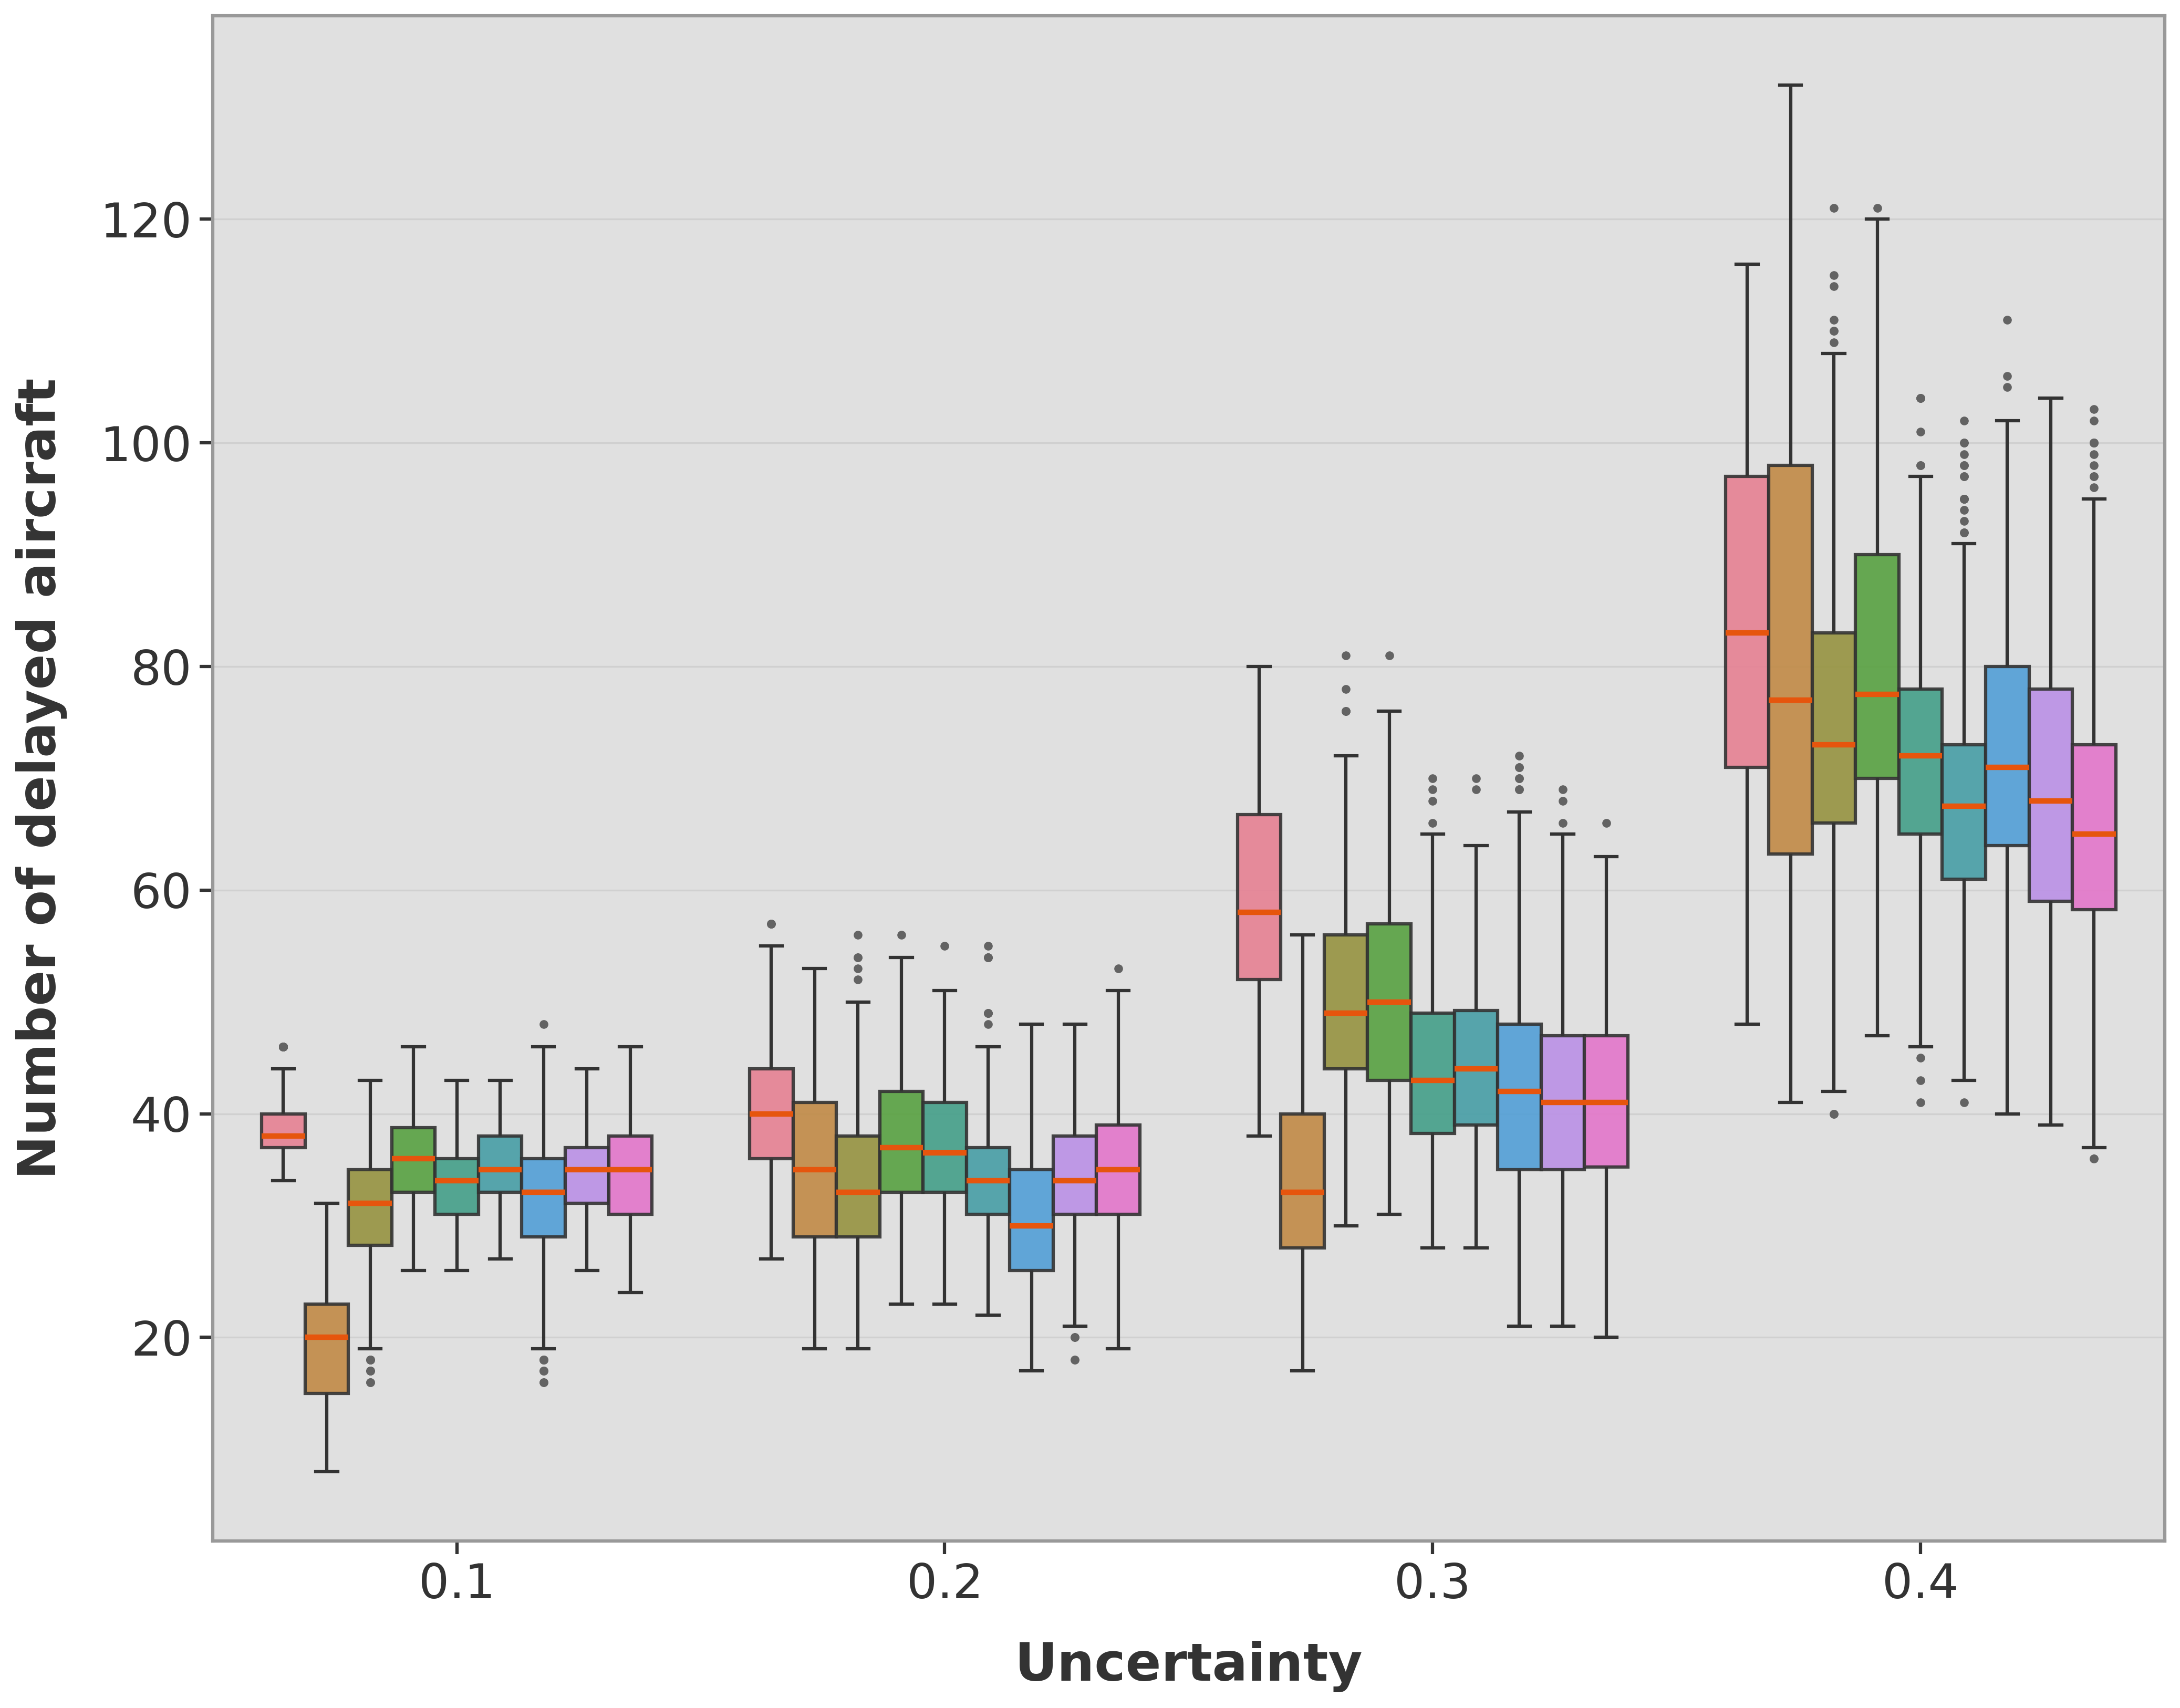
\includegraphics[width=0.45\textwidth]{figures/Traffic_1.1/traffic_1.1_delayed_30s_count.png}} 
%     \subfigure(e){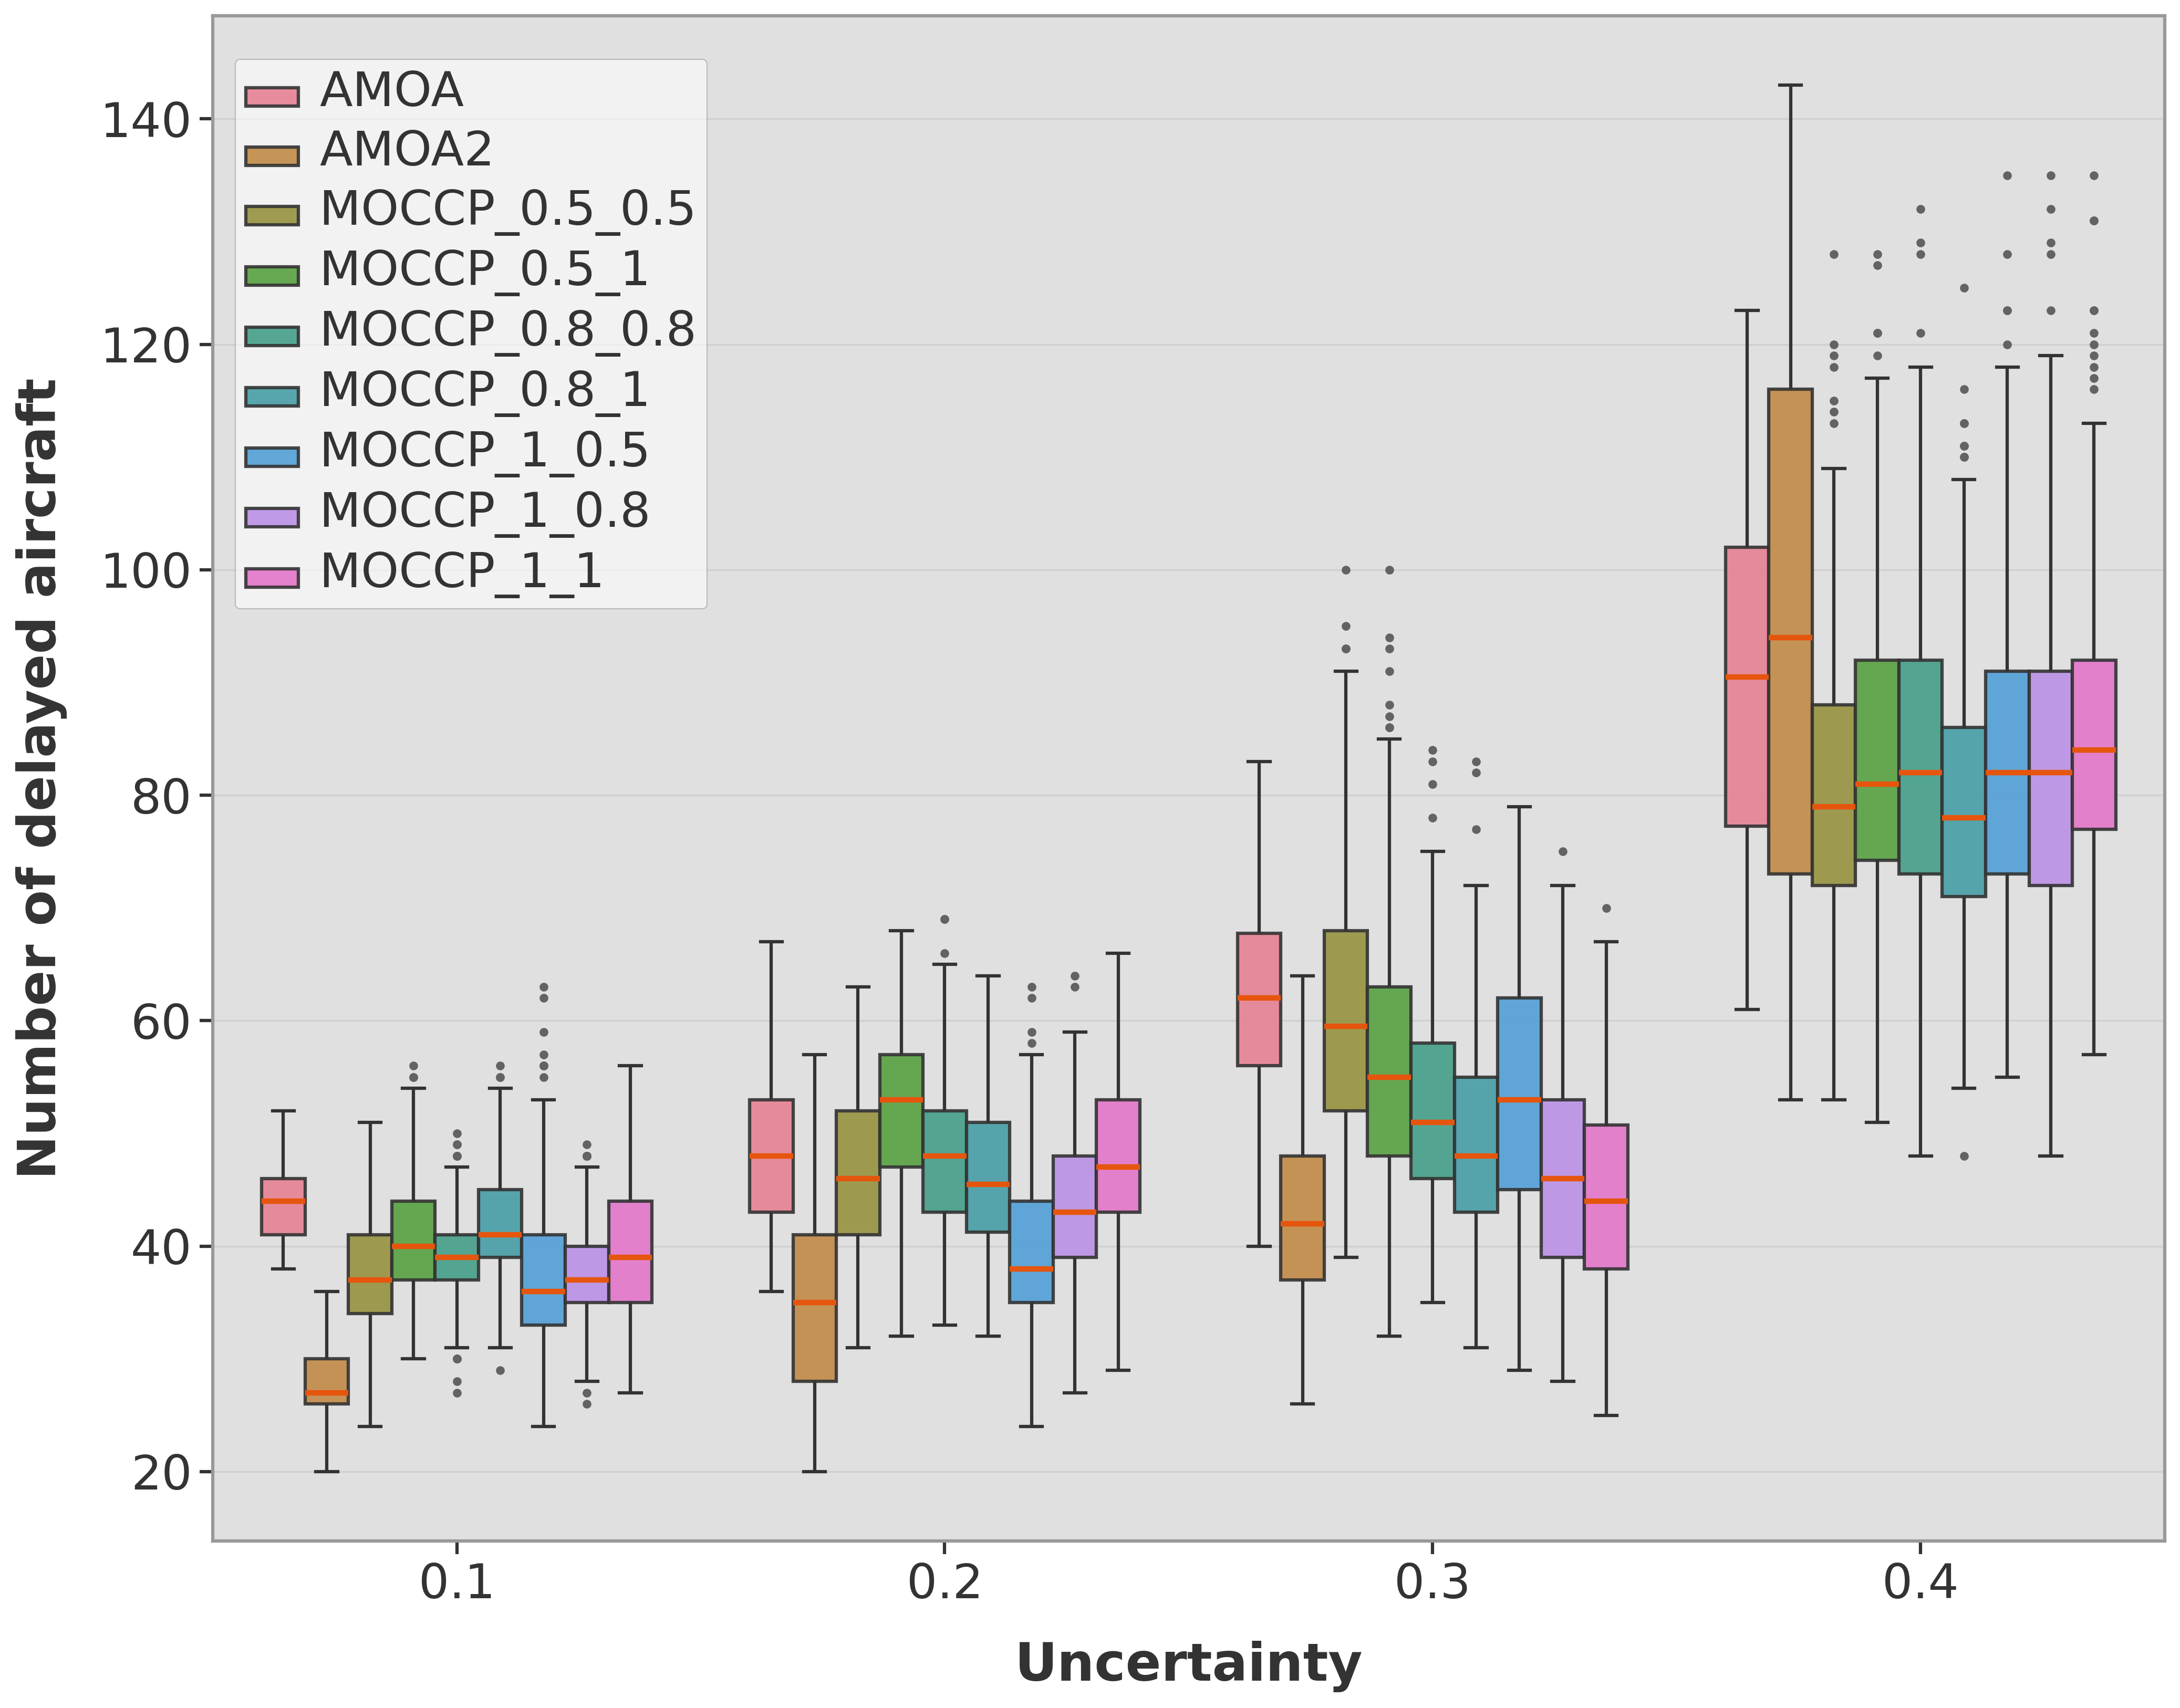
\includegraphics[width=0.45\textwidth]{figures/Traffic_1.2/traffic_1.2_delayed_30s_count.png}} 
%     \caption{Number of delayed aircraft under different traffic densities. Sub figures (a)–(e) correspond to traffic densities of 0.8, 0.9, 1.0, 1.1, and 1.2, respectively. And in each sub figure, each group of nine bars has the same level of uncertainties.}
%     \label{fig:nda}
% \end{figure}

% \begin{figure}[htp]
%     \centering
%     \subfigure(a){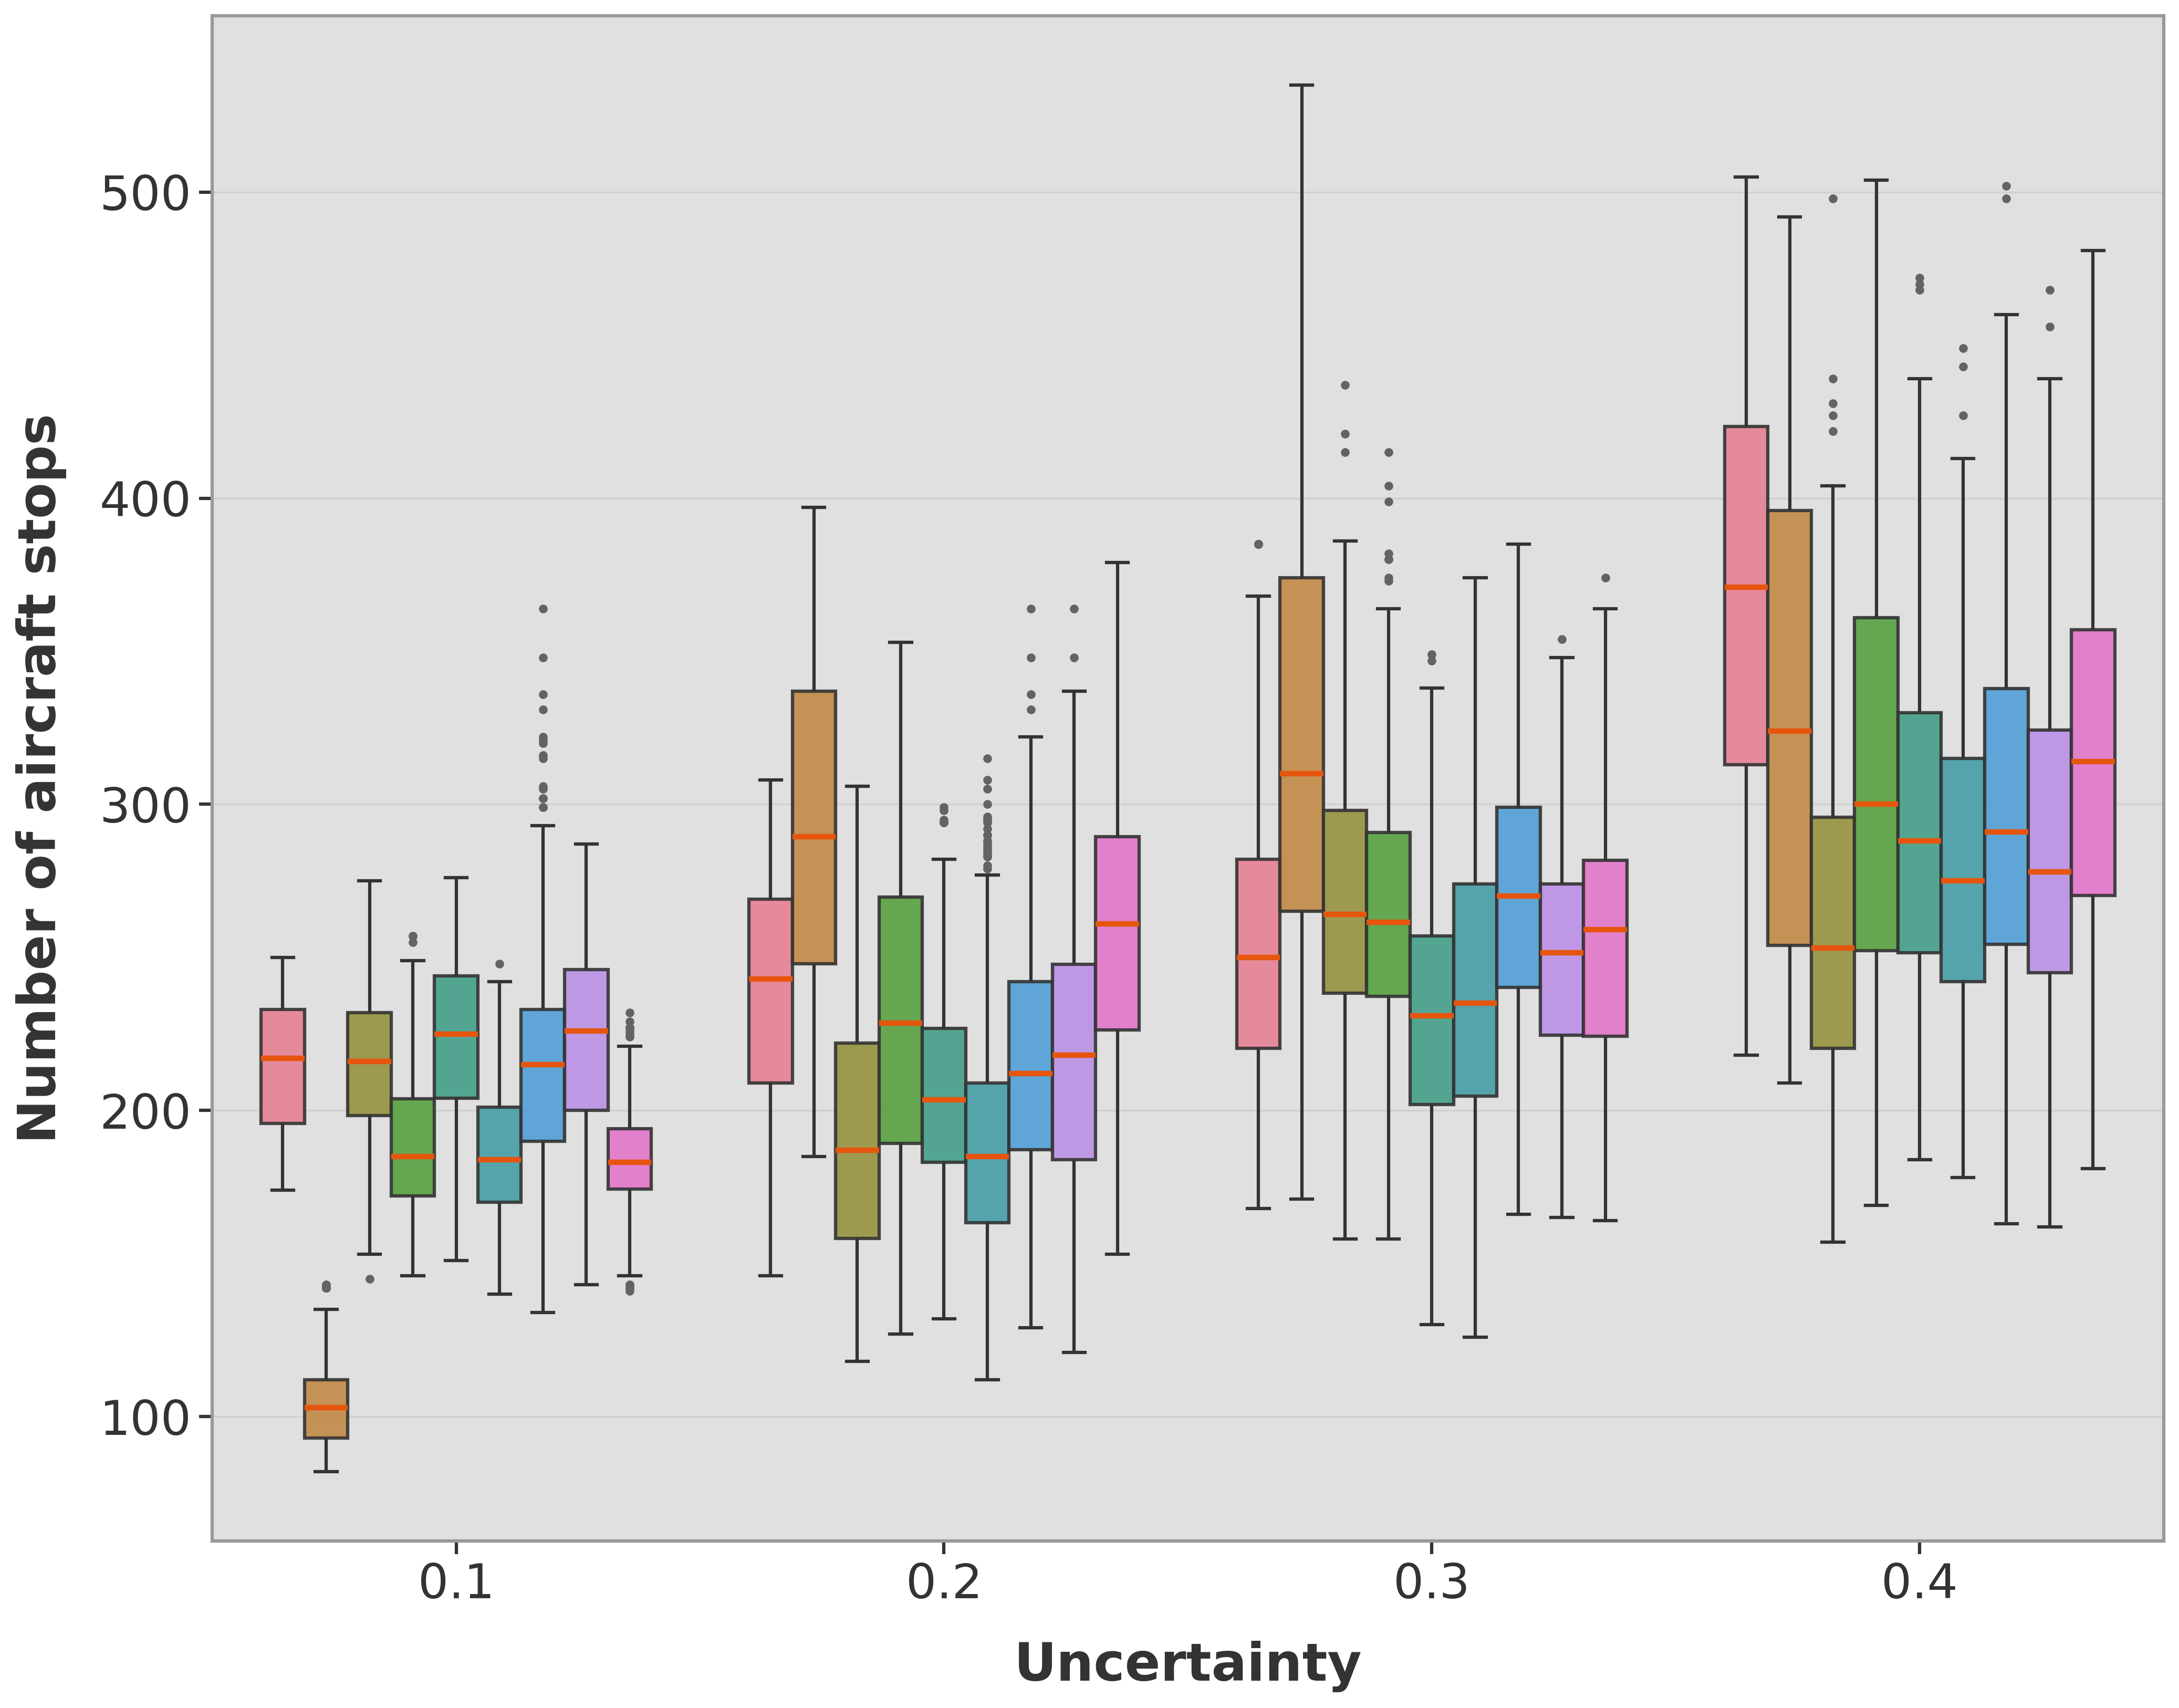
\includegraphics[width=0.45\textwidth]{figures/Traffic_0.8/traffic_0.8_num_waits.png}} 
%     \subfigure(b){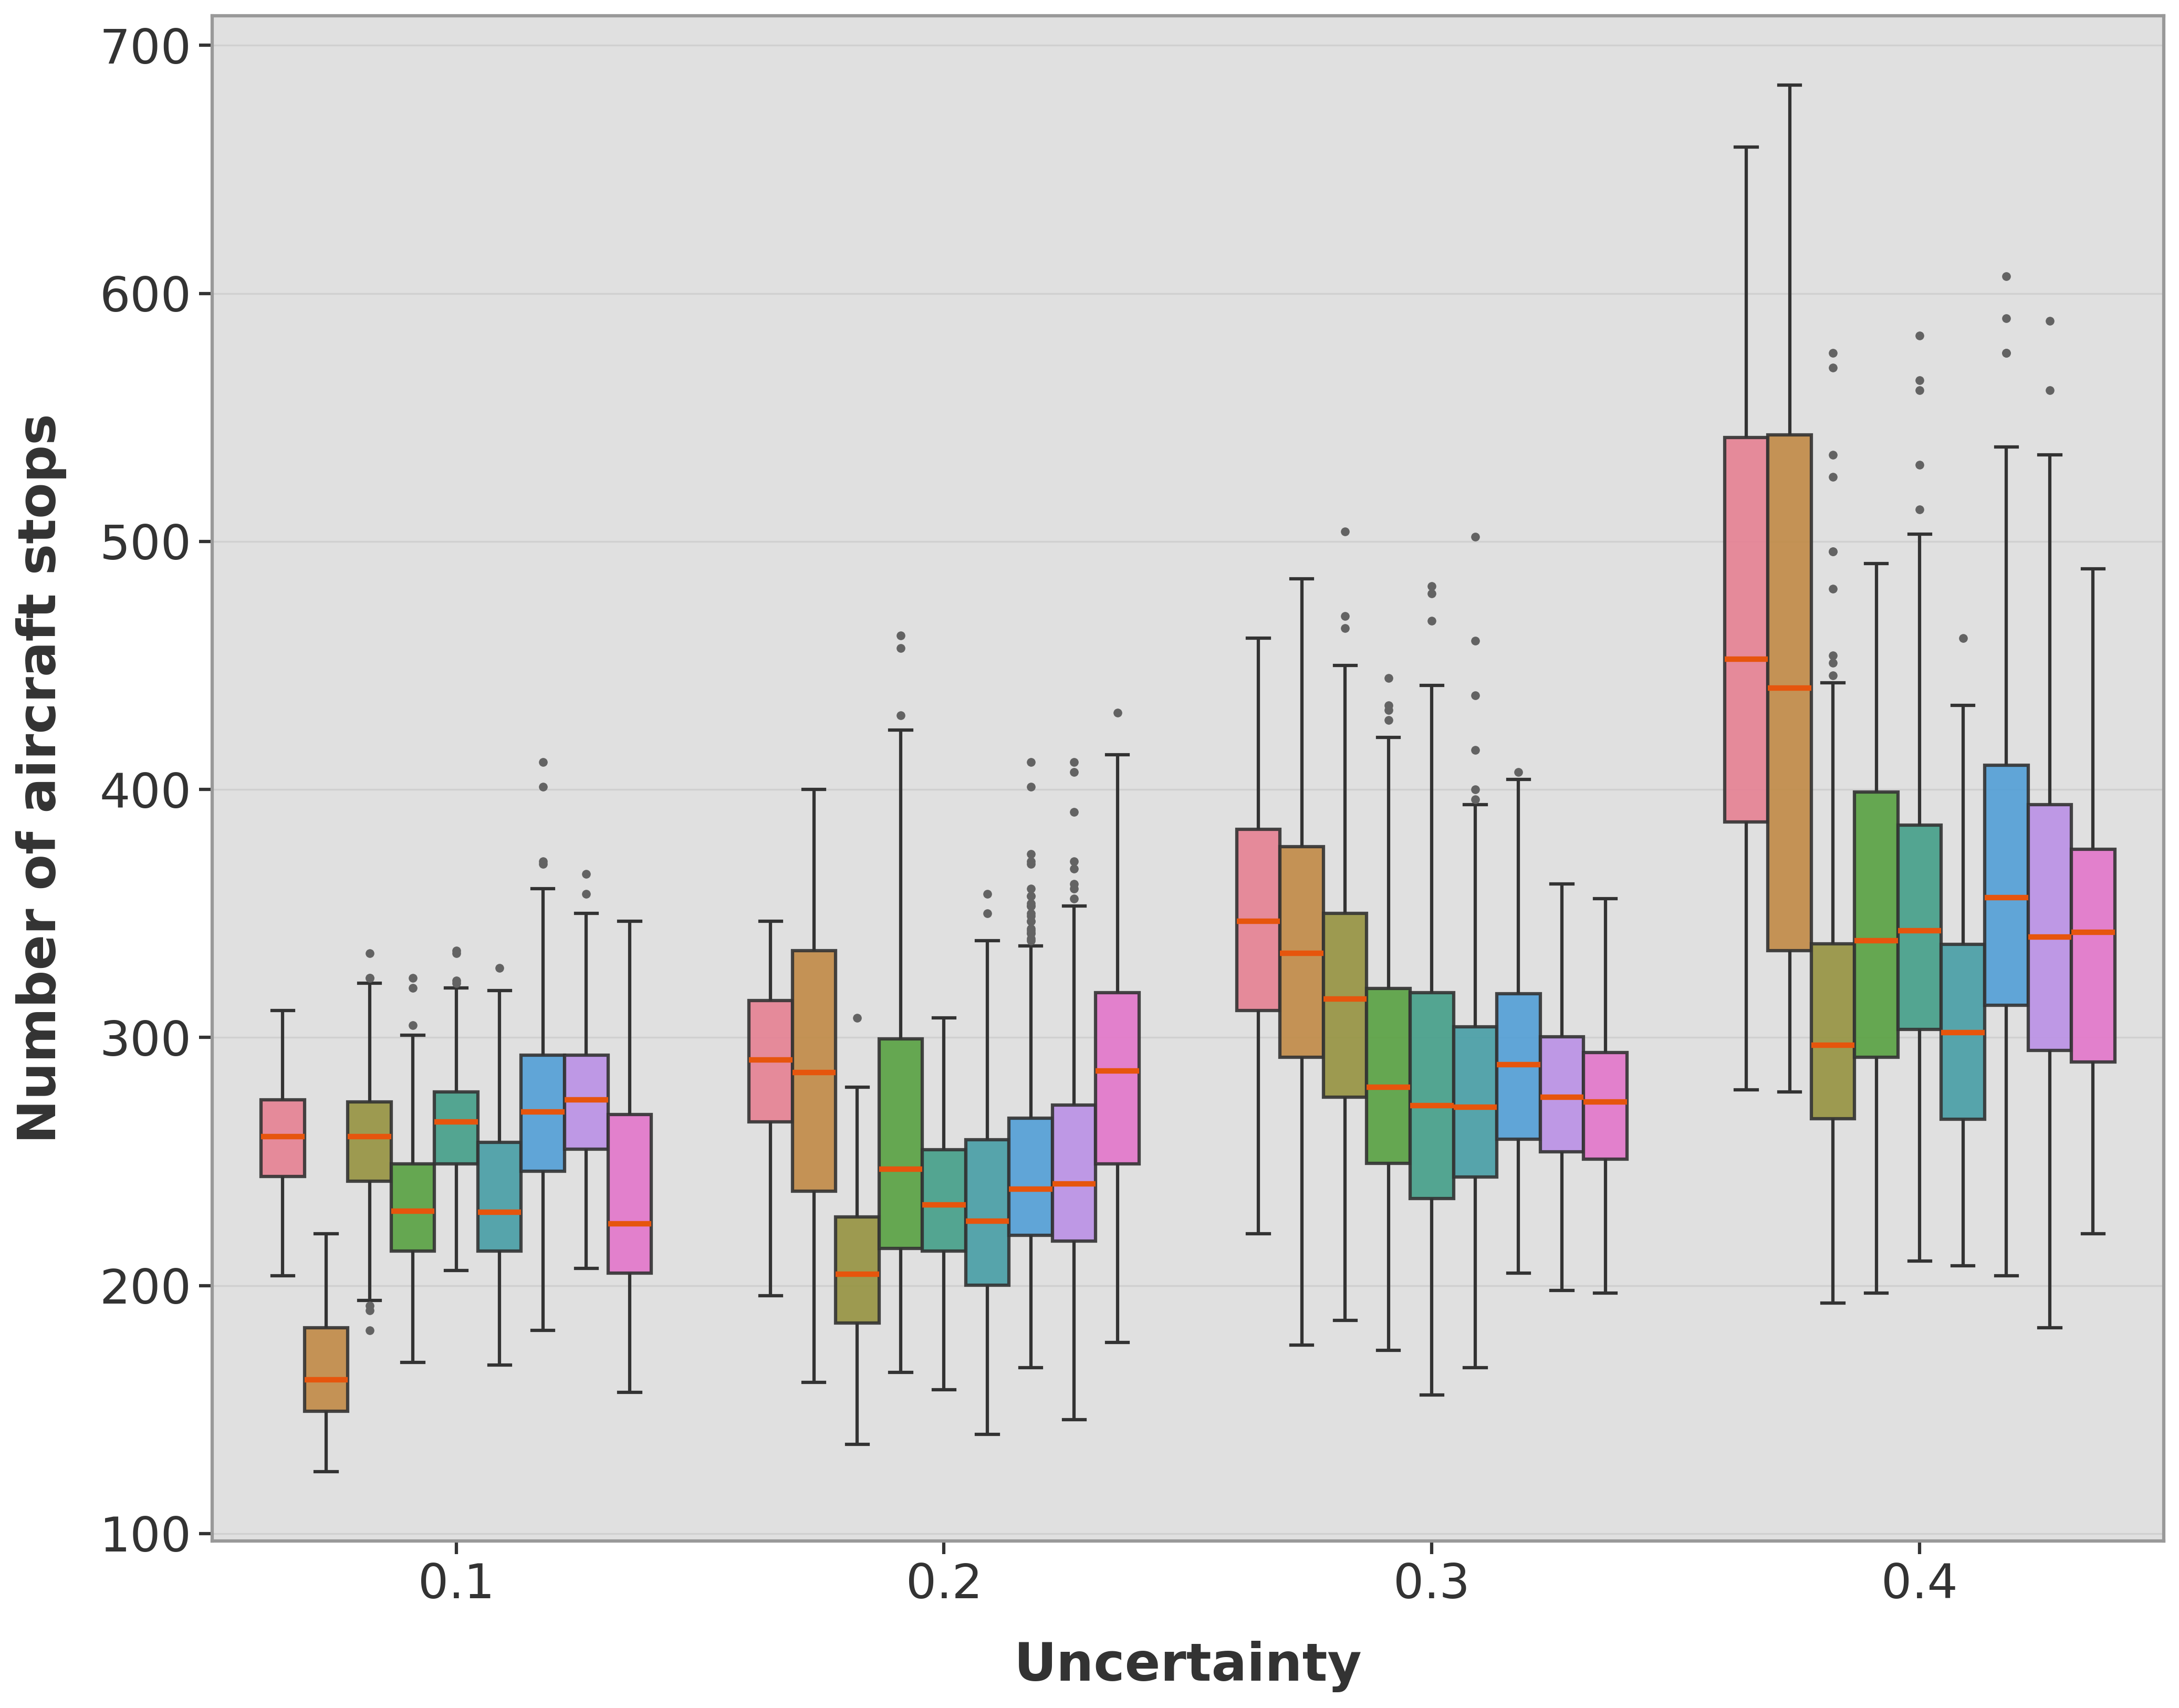
\includegraphics[width=0.45\textwidth]{figures/Traffic_0.9/traffic_0.9_num_waits.png}} 
%     \subfigure(c){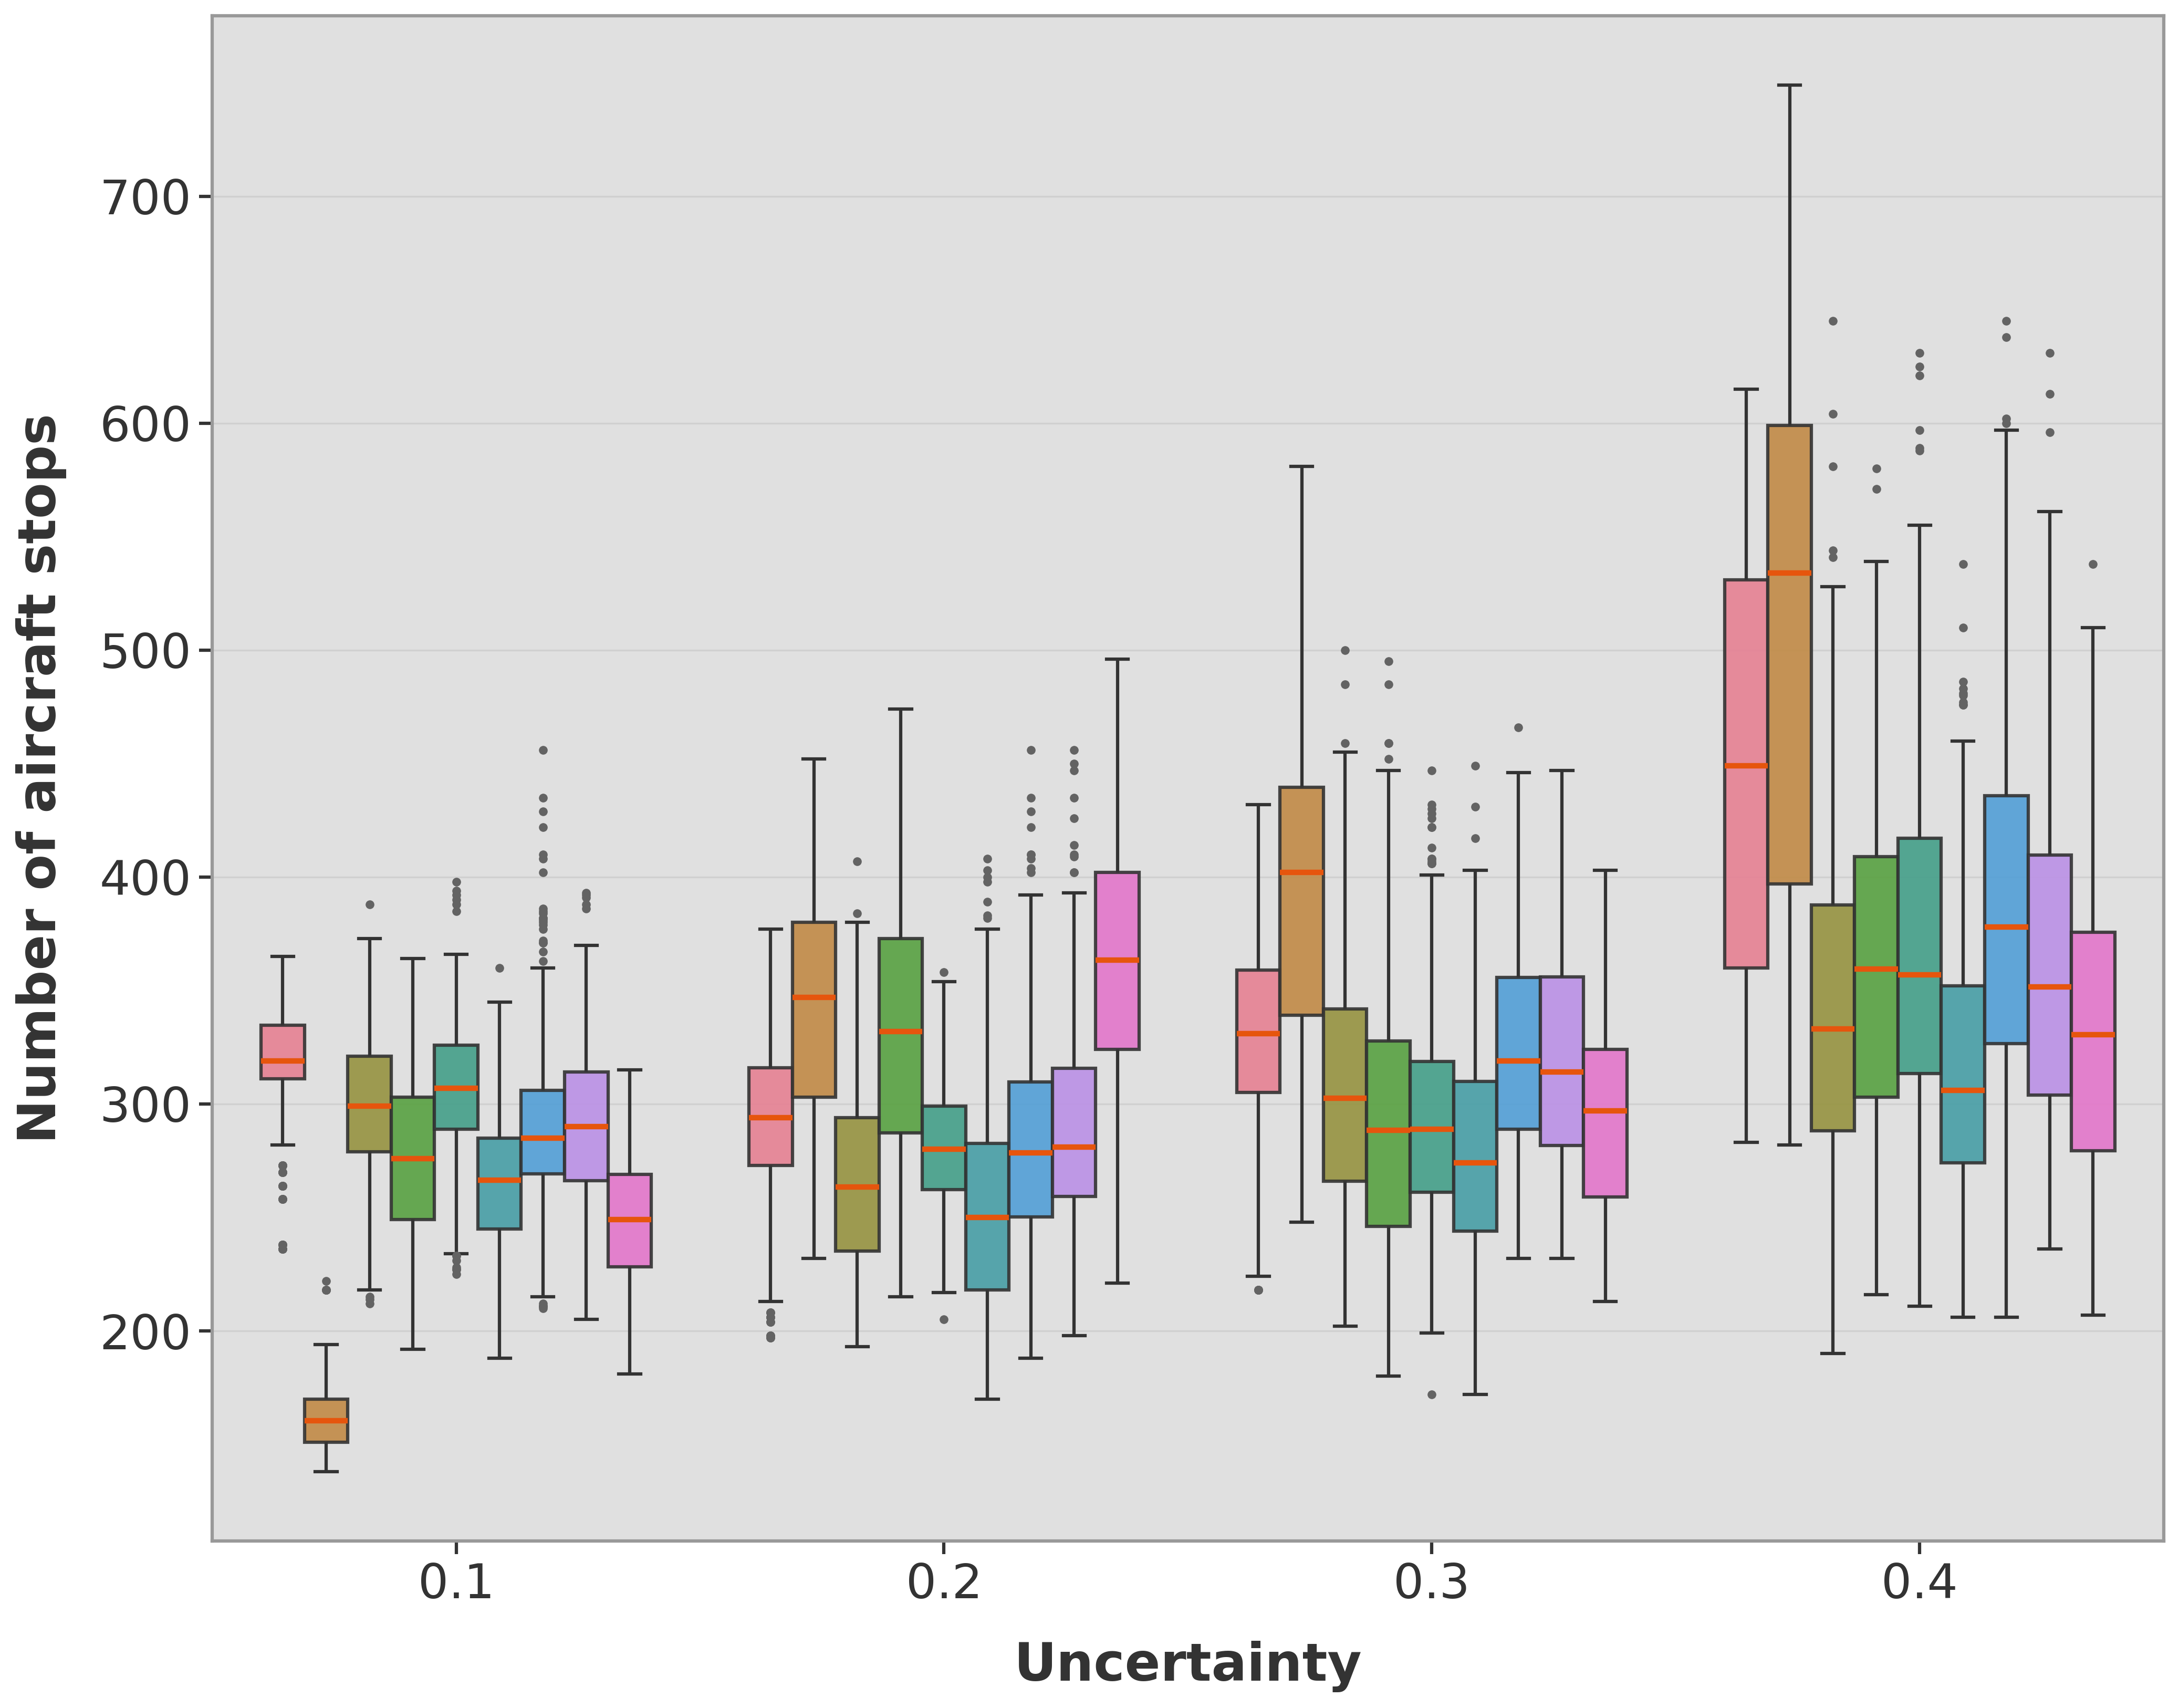
\includegraphics[width=0.45\textwidth]{figures/Traffic_1.0/traffic_1.0_num_waits.png}} 
%       \subfigure(d){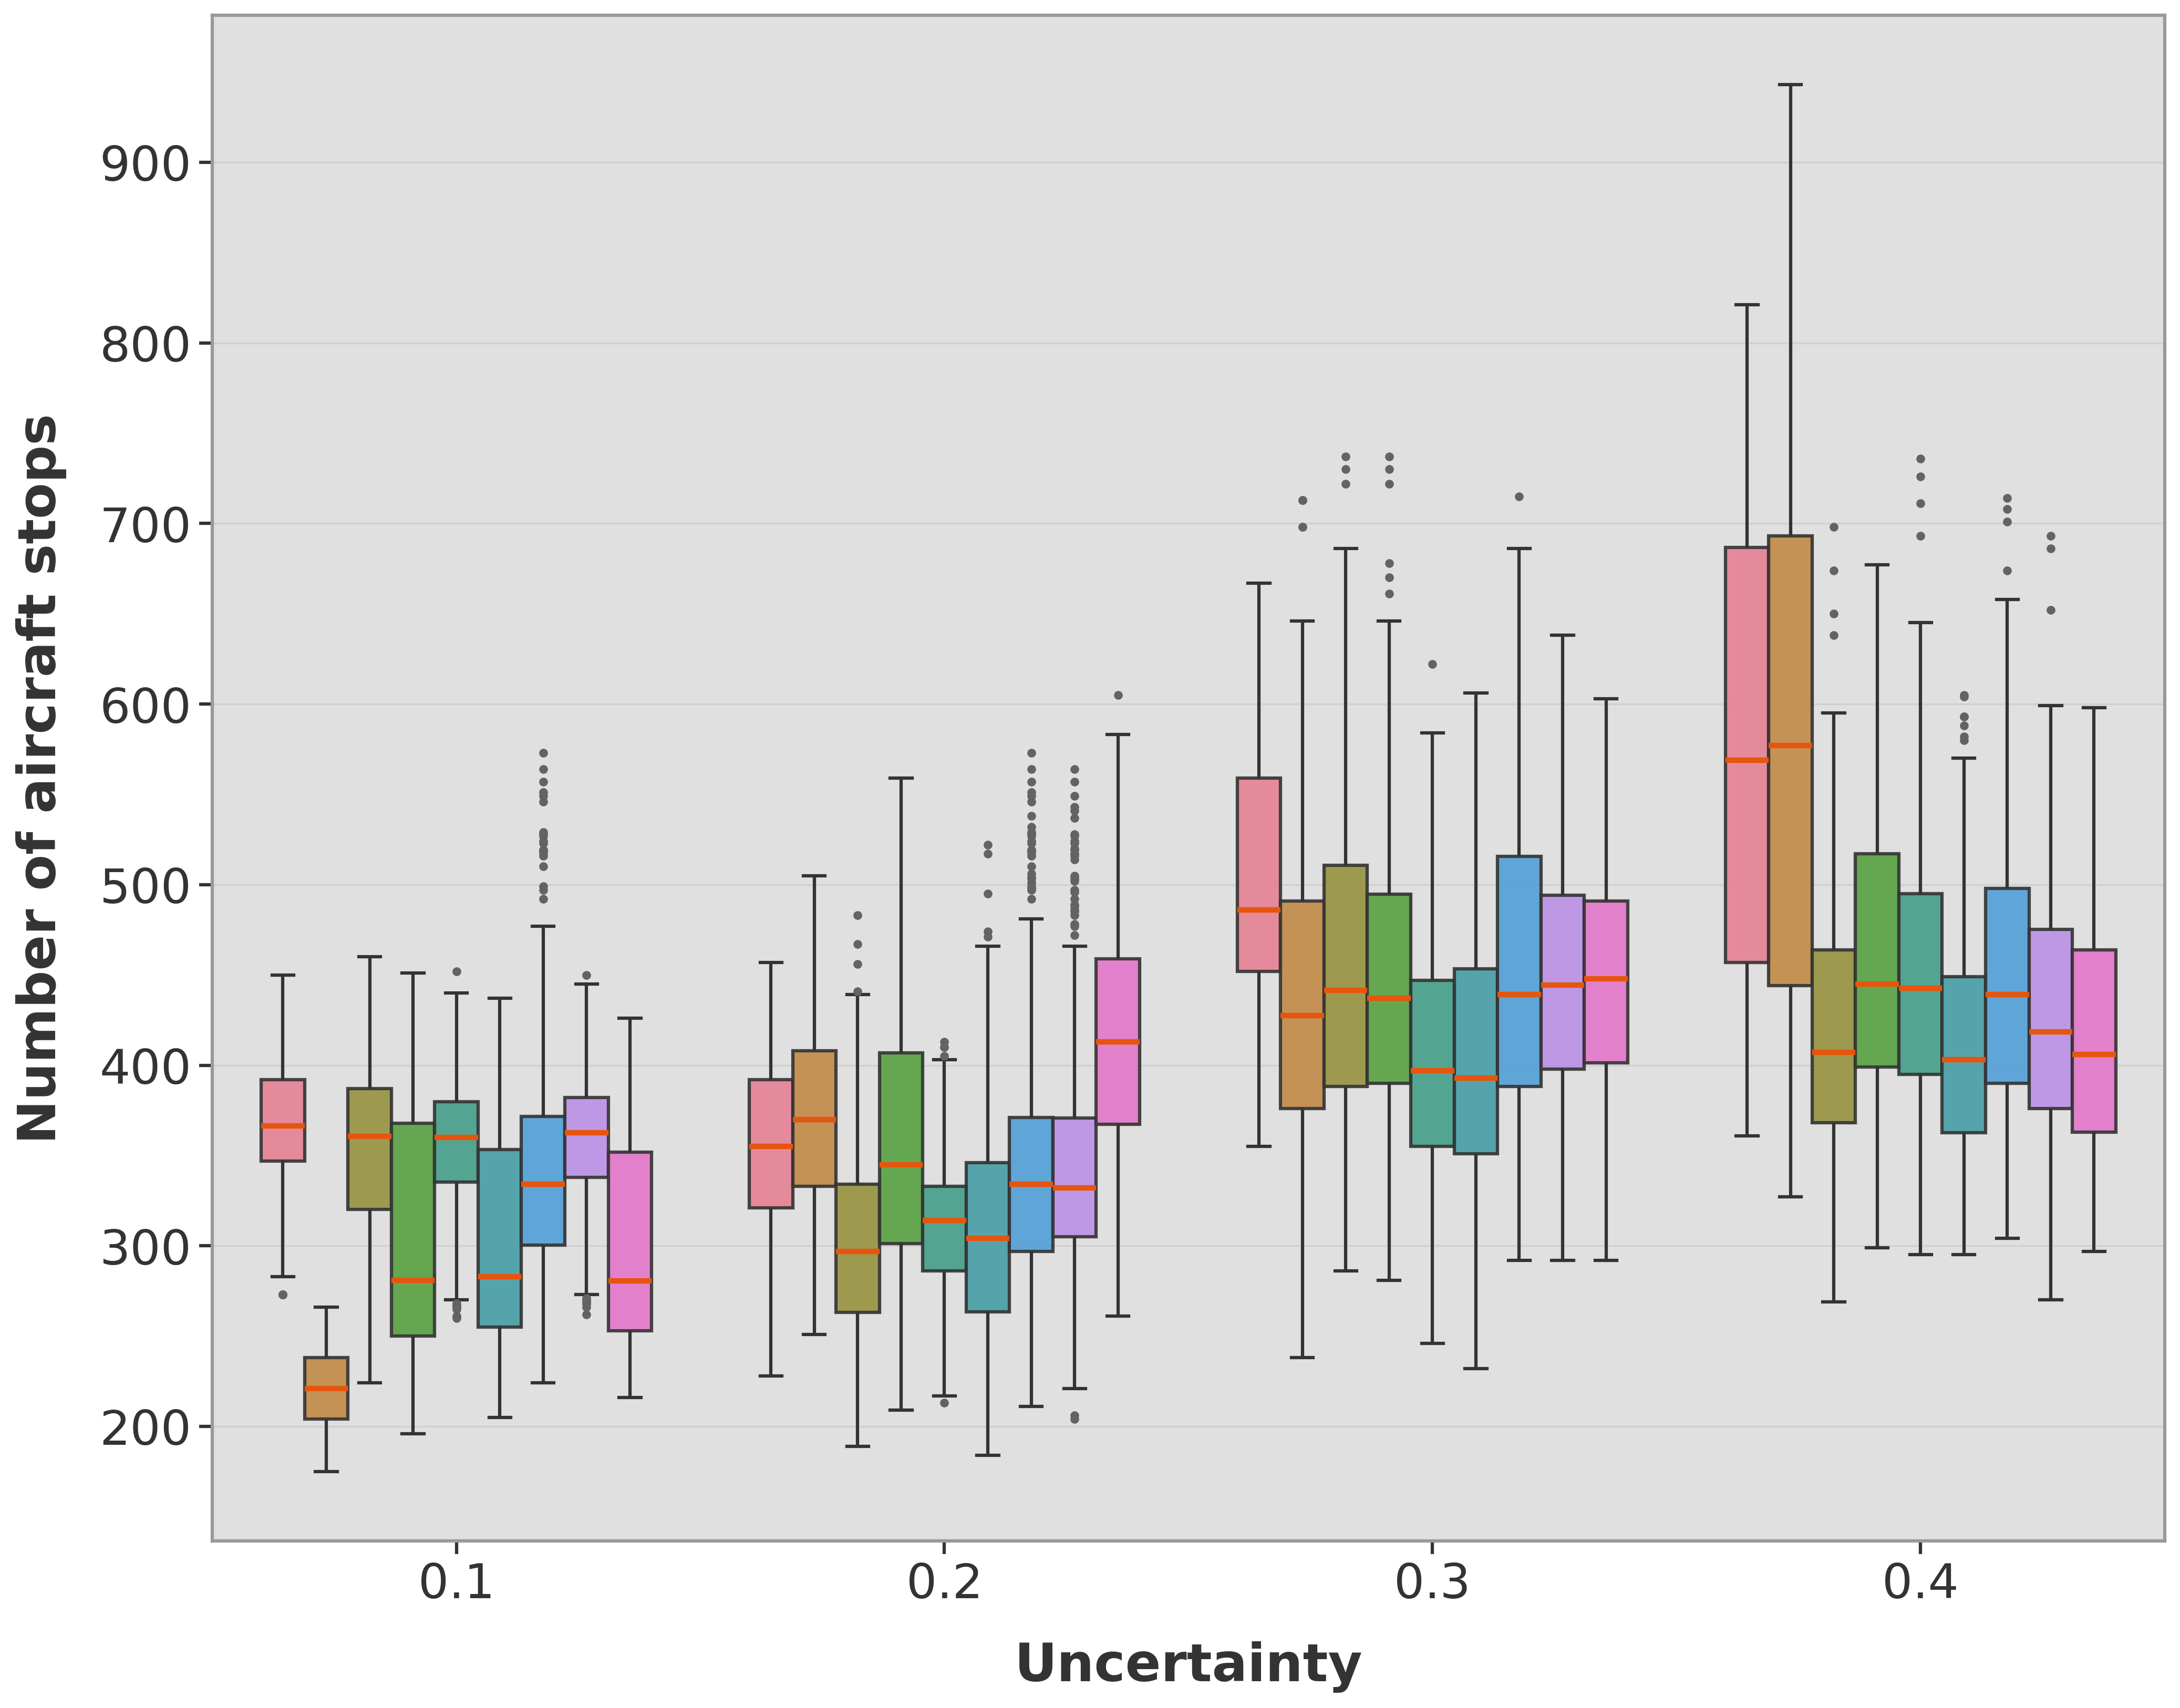
\includegraphics[width=0.45\textwidth]{figures/Traffic_1.1/traffic_1.1_num_waits.png}} 
%     \subfigure(e){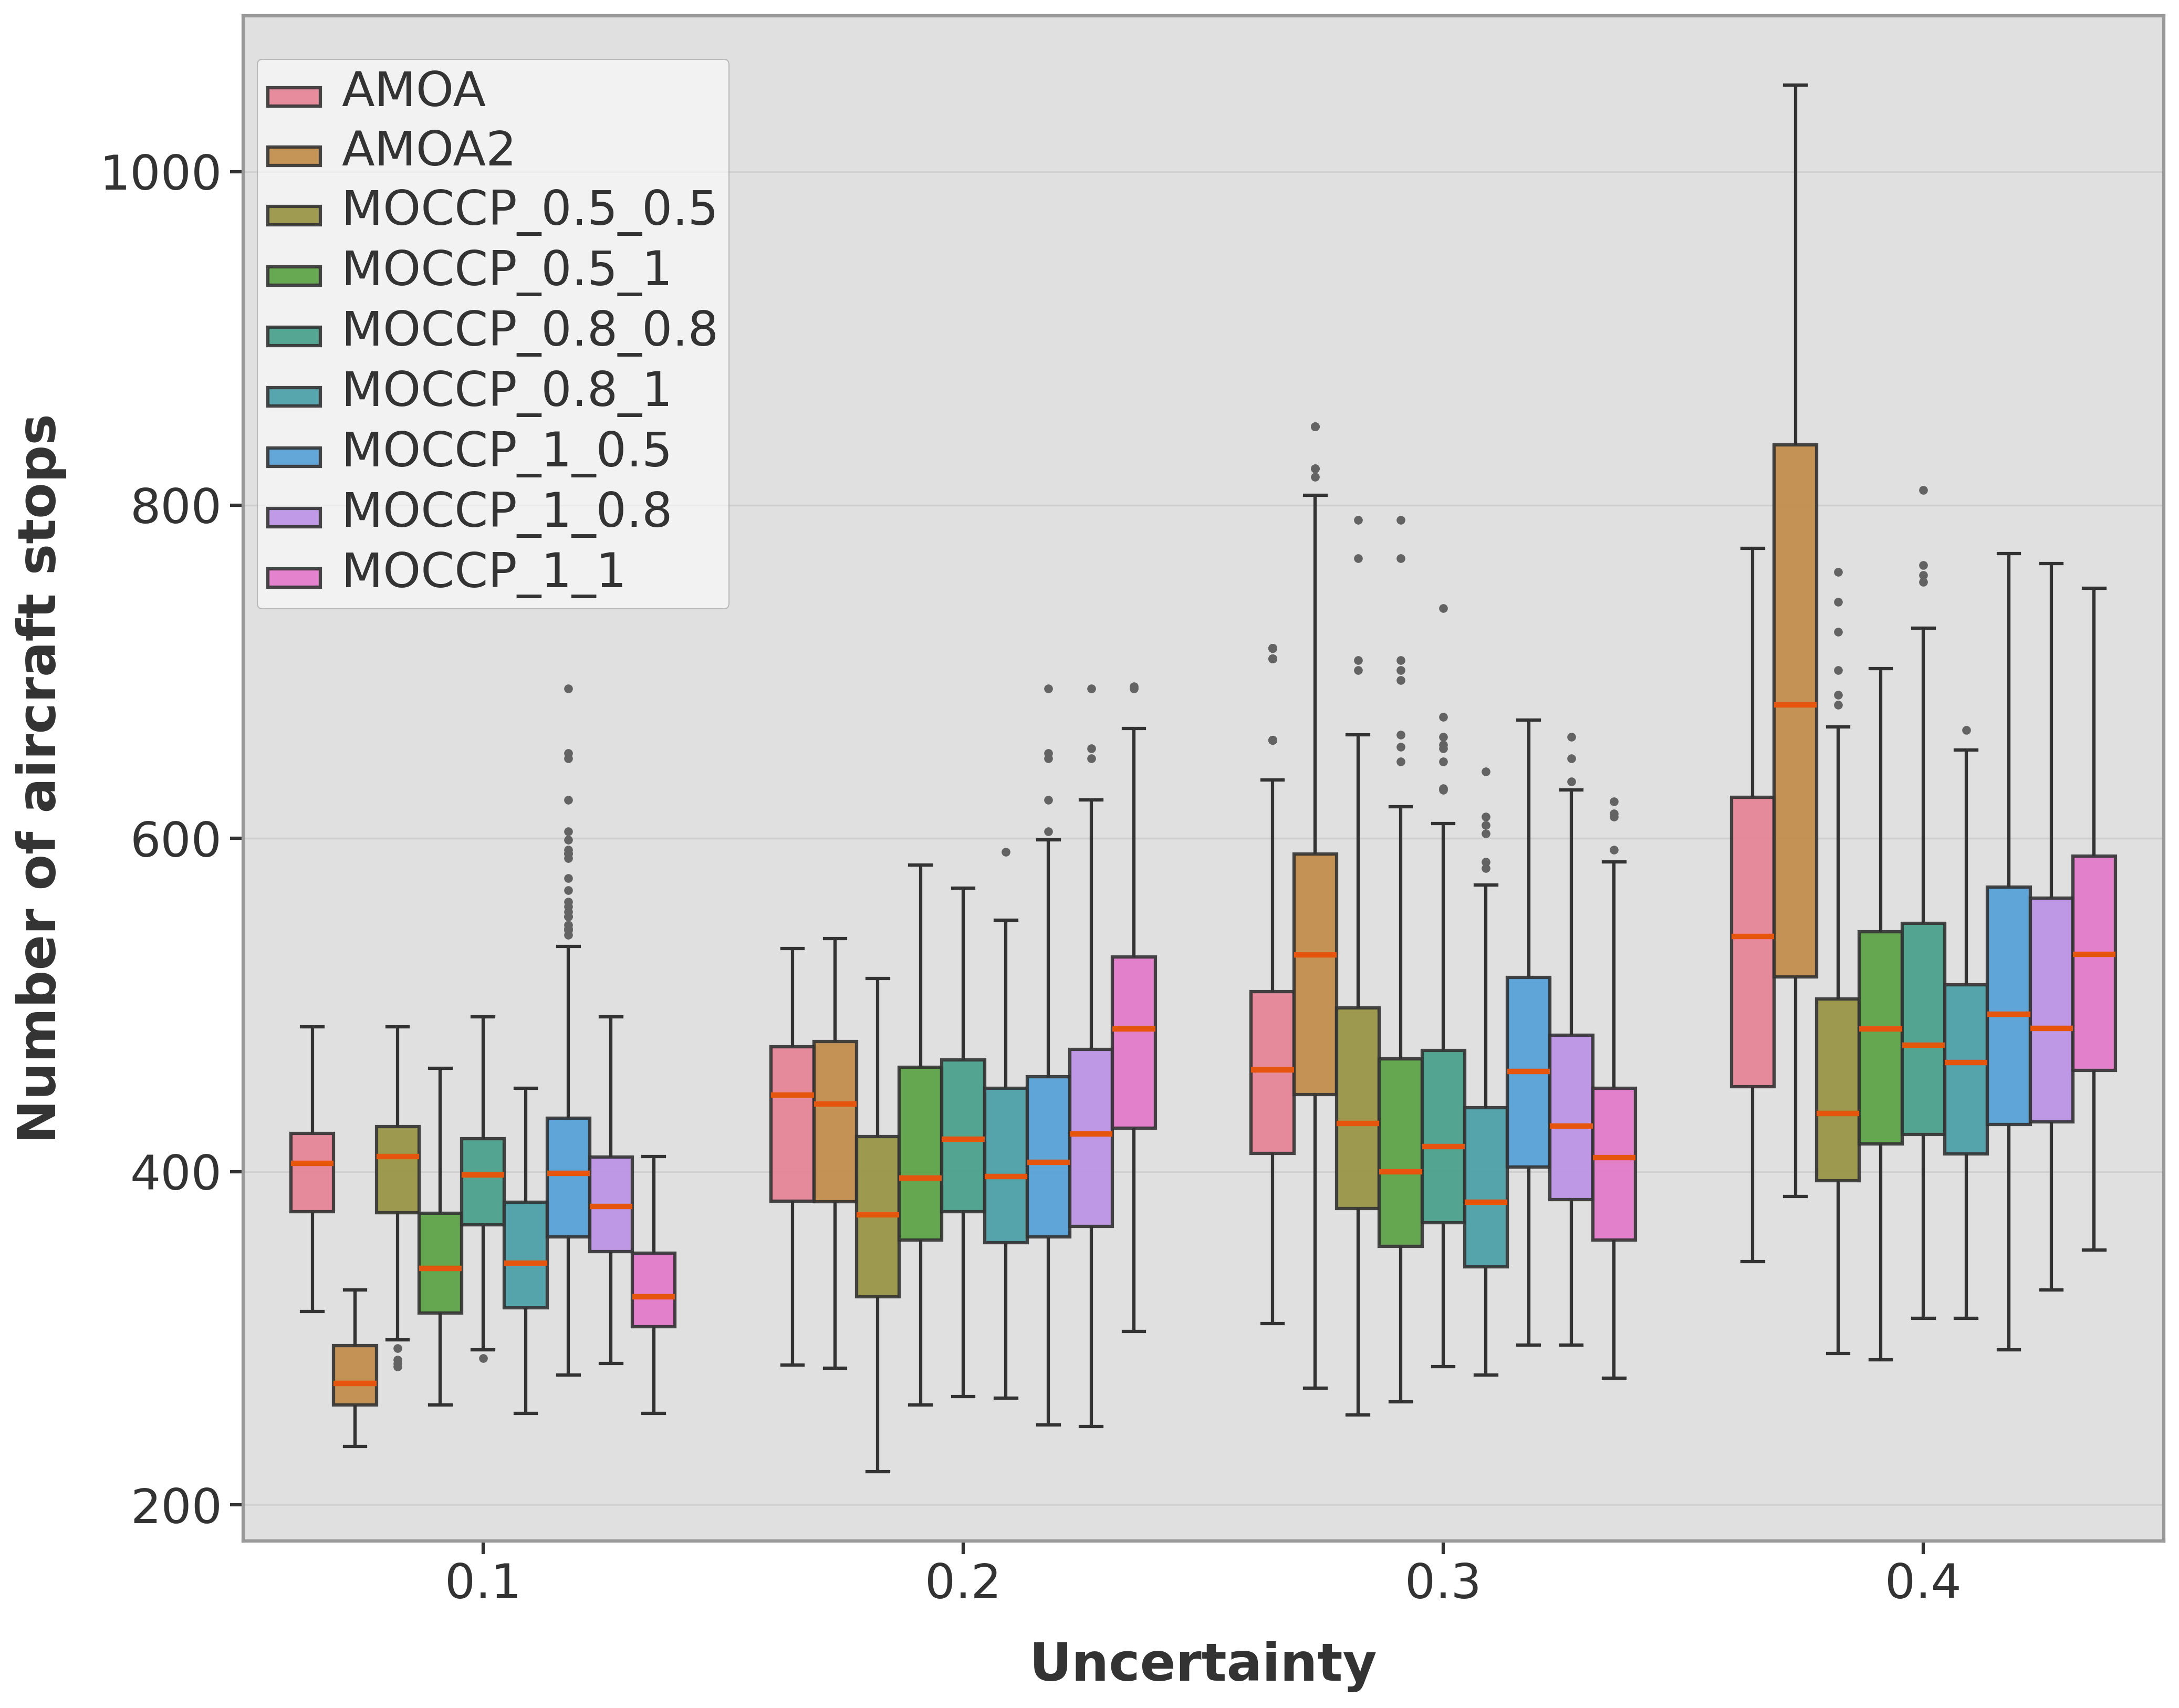
\includegraphics[width=0.45\textwidth]{figures/Traffic_1.2/traffic_1.2_num_waits.png}} 
%     \caption{Number of aircraft stops under different traffic densities. Sub figures (a)–(e) correspond to traffic densities of 0.8, 0.9, 1.0, 1.1, and 1.2, respectively. And in each sub figure, each group of nine bars has the same level of uncertainties.}
%     \label{fig:nas}
% \end{figure}

Fig.~\ref{fig:delay} presents the distributions of total delay across varying uncertainty levels from 0.1 to 0.4, and five traffic densities  from 0.8 to 1.2. As expected, total delay increases with higher uncertainty levels, with this effect becoming more pronounced under denser traffic conditions. Among all evaluated algorithms, \texttt{amoa} yields the highest average delays, whereas \texttt{amoa2} generally performs the best except under an uncertainty level of 0.4. This outcome can be explained by the fact that \texttt{amoa2} employs worst-case estimates for taxiing time, which might help avoid conflicts through strategic detours. In contrast, \texttt{amoa}, which relies on average values, is less effective in mitigating taxiing congestion. Despite its overall strong performance, \texttt{amoa2} exhibits higher delay variability under an uncertainty level of 0.4 and higher average delays at traffic densities of 0.9 and 1.0 (Figs.~\ref{fig:delay_b},~\ref{fig:delay_c}), indicating reduced effectiveness under highly uncertain conditions. In contrast, as both uncertainties and congestion intensify, the CCP-AMOA* algorithms exhibit superior robustness in maintaining solution stability. Specifically, algorithms with higher confidence levels in taxiing time (e.g., \texttt{moccp\_1\_0.5}, \texttt{moccp\_1\_1}) achieve relatively low and more stable delays, suggesting that conservative control over taxiing time helps mitigate delay propagation throughout the airport surface, especially in complex and uncertain operational environments. 

\begin{figure}[htp]
    \centering
    
    % Row 1
    \subfloat[Traffic density = 0.8\label{fig:delay_a}]{
        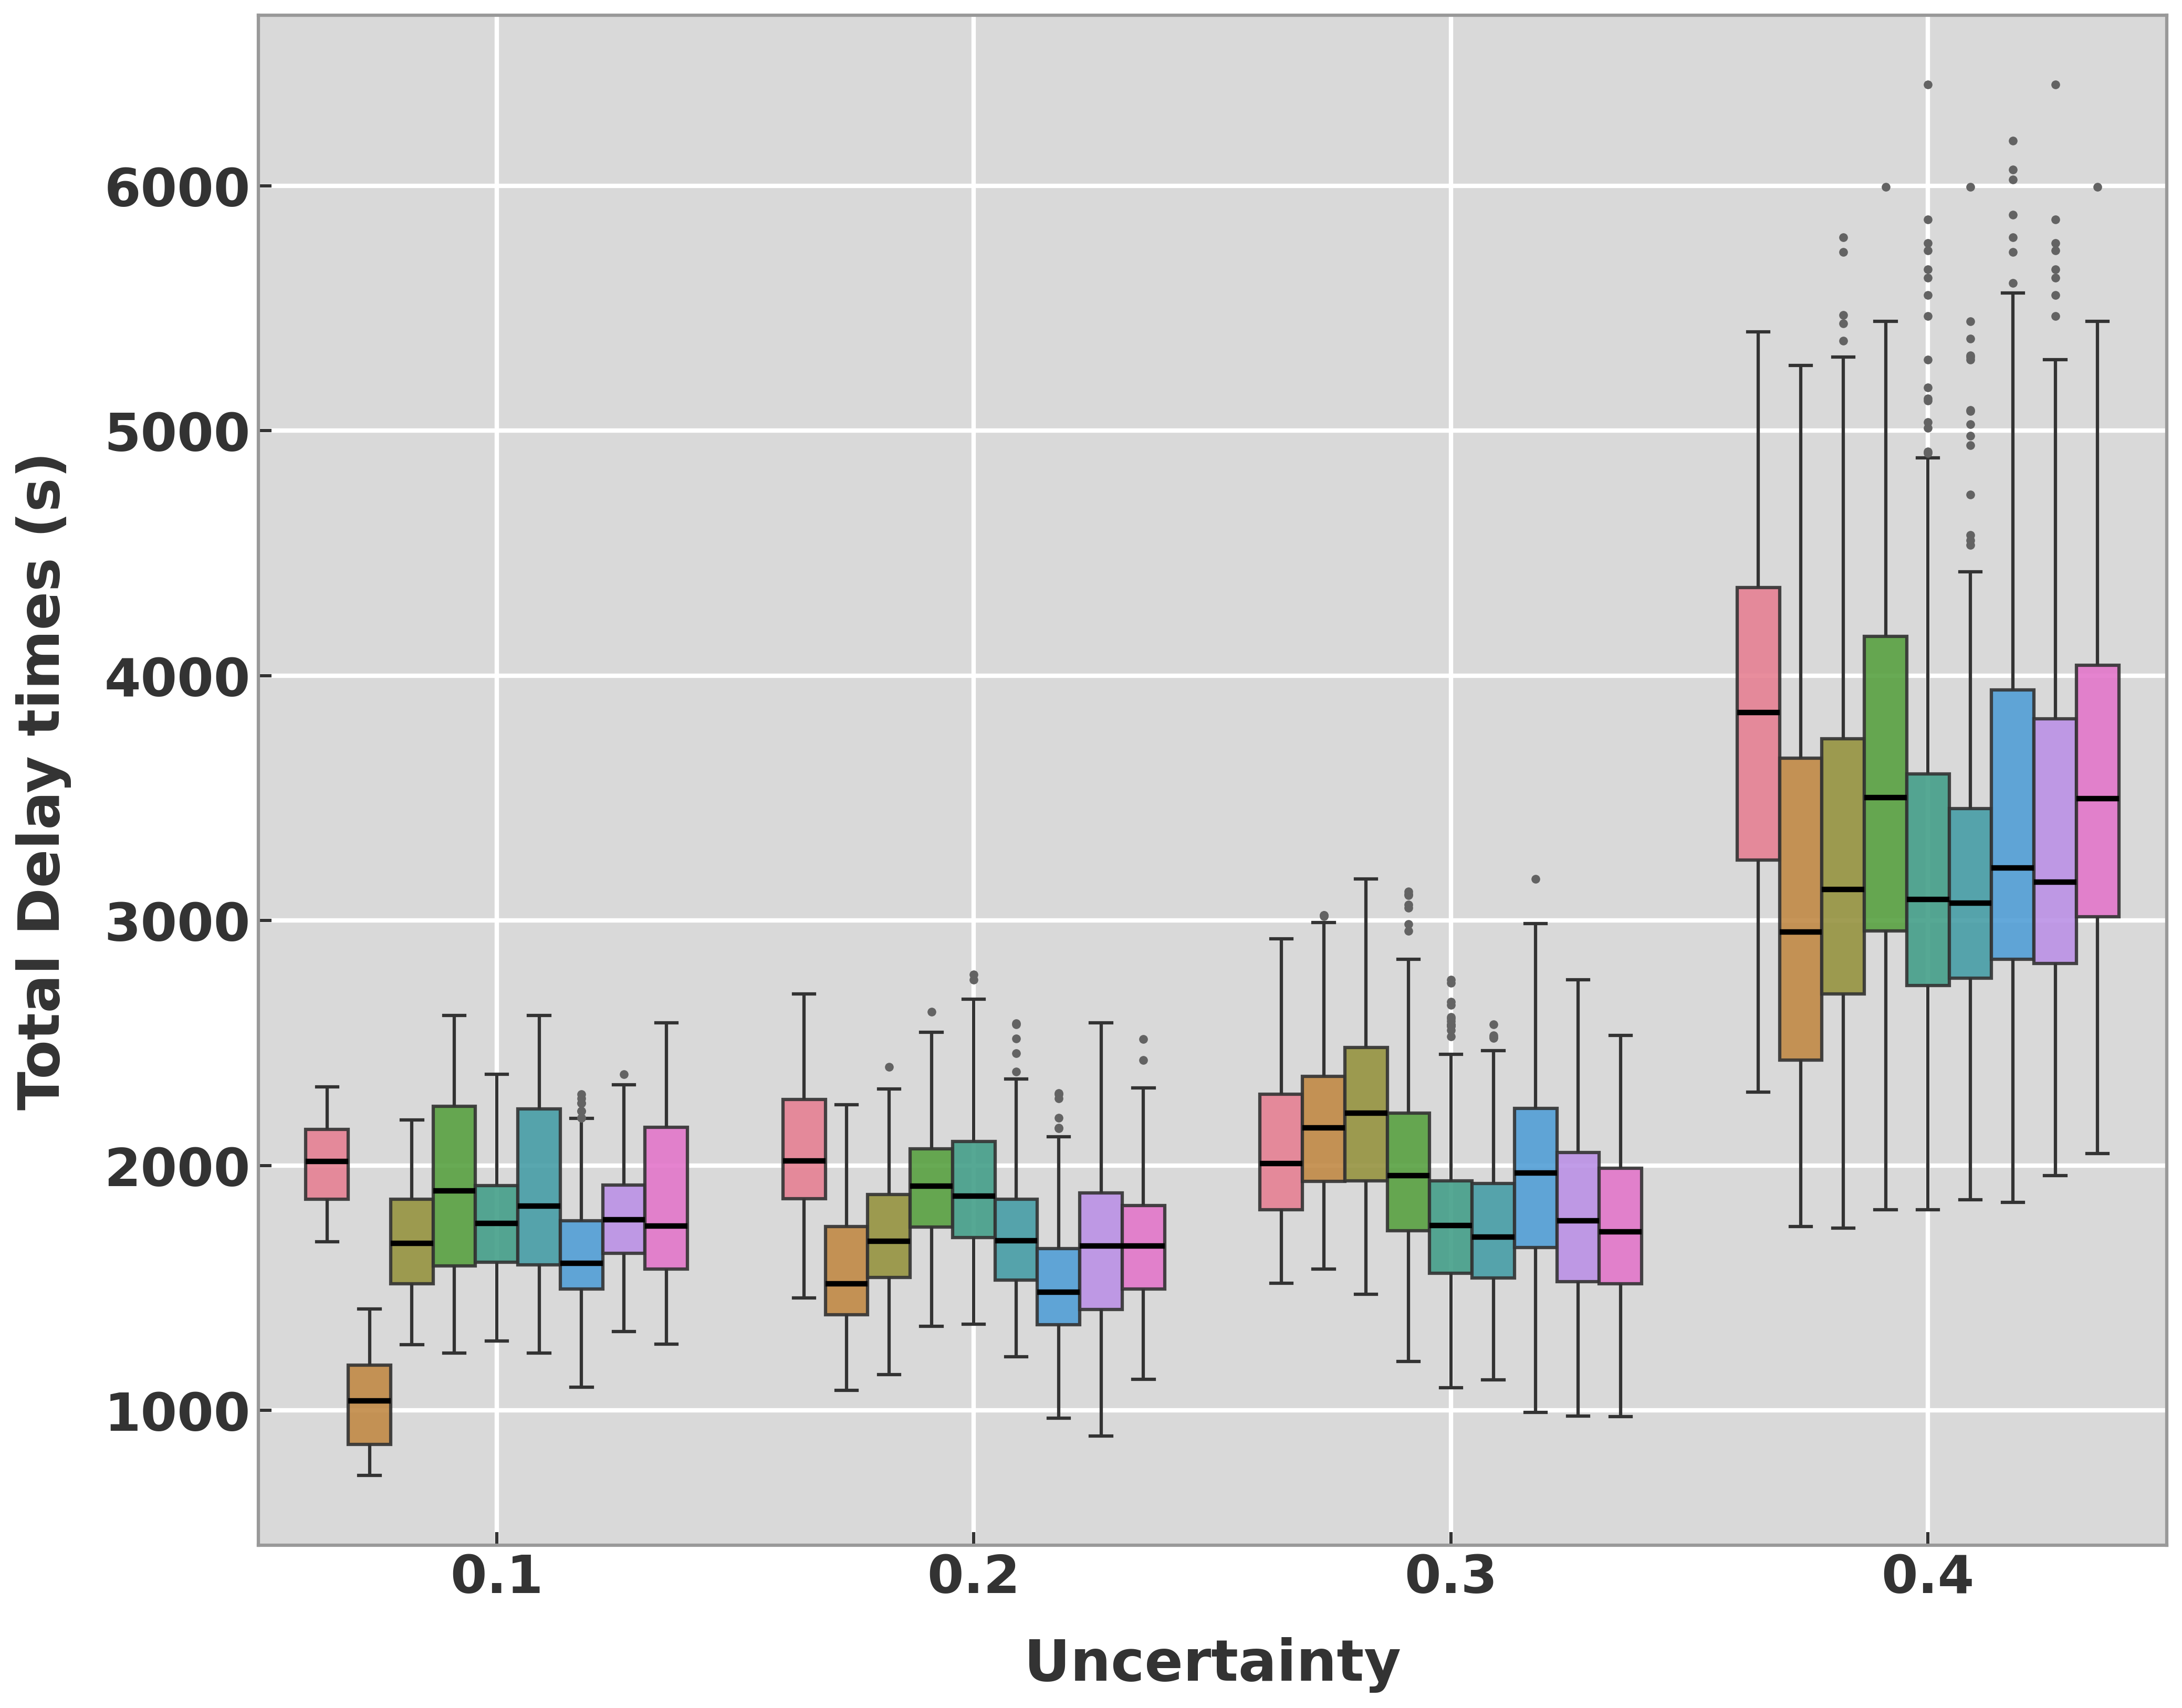
\includegraphics[width=0.45\textwidth]{figures/Traffic_0.8/traffic_0.8_total_delay.png}
    }
    \hfill
    \subfloat[Traffic density = 0.9\label{fig:delay_b}]{
        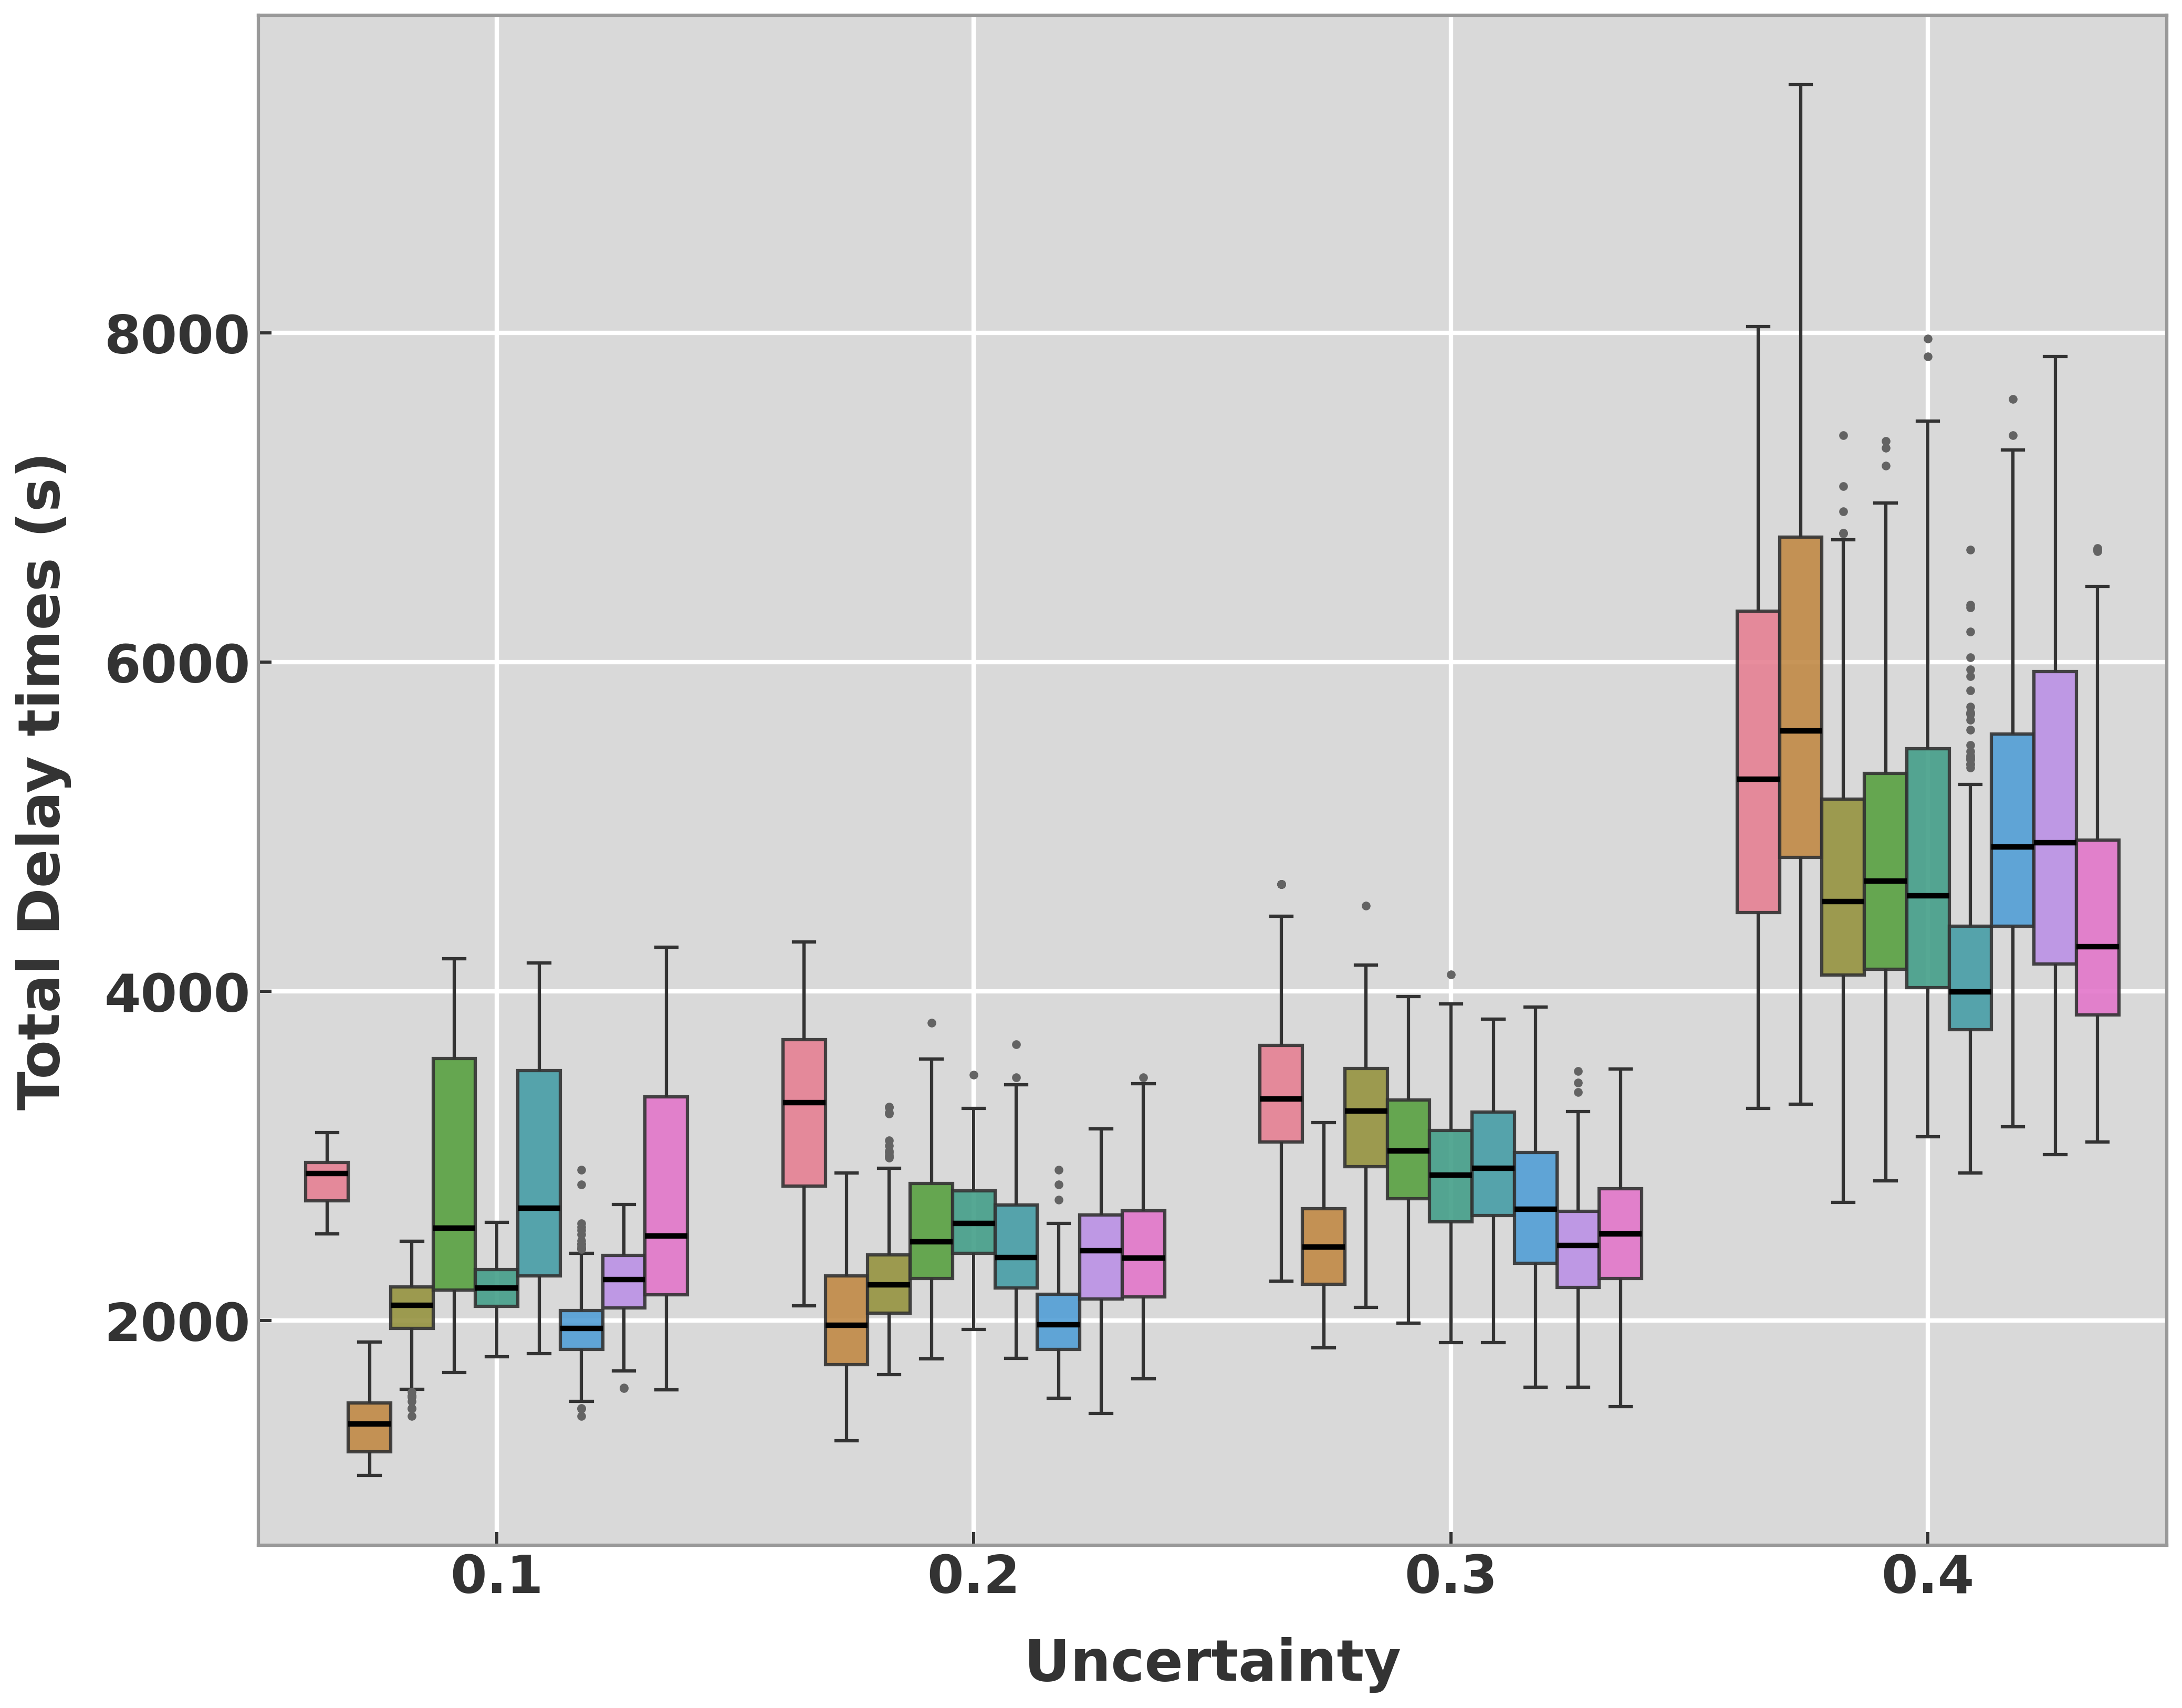
\includegraphics[width=0.45\textwidth]{figures/Traffic_0.9/traffic_0.9_total_delay.png}
    }
    
    % Row 2
    \subfloat[Traffic density = 1.0\label{fig:delay_c}]{
        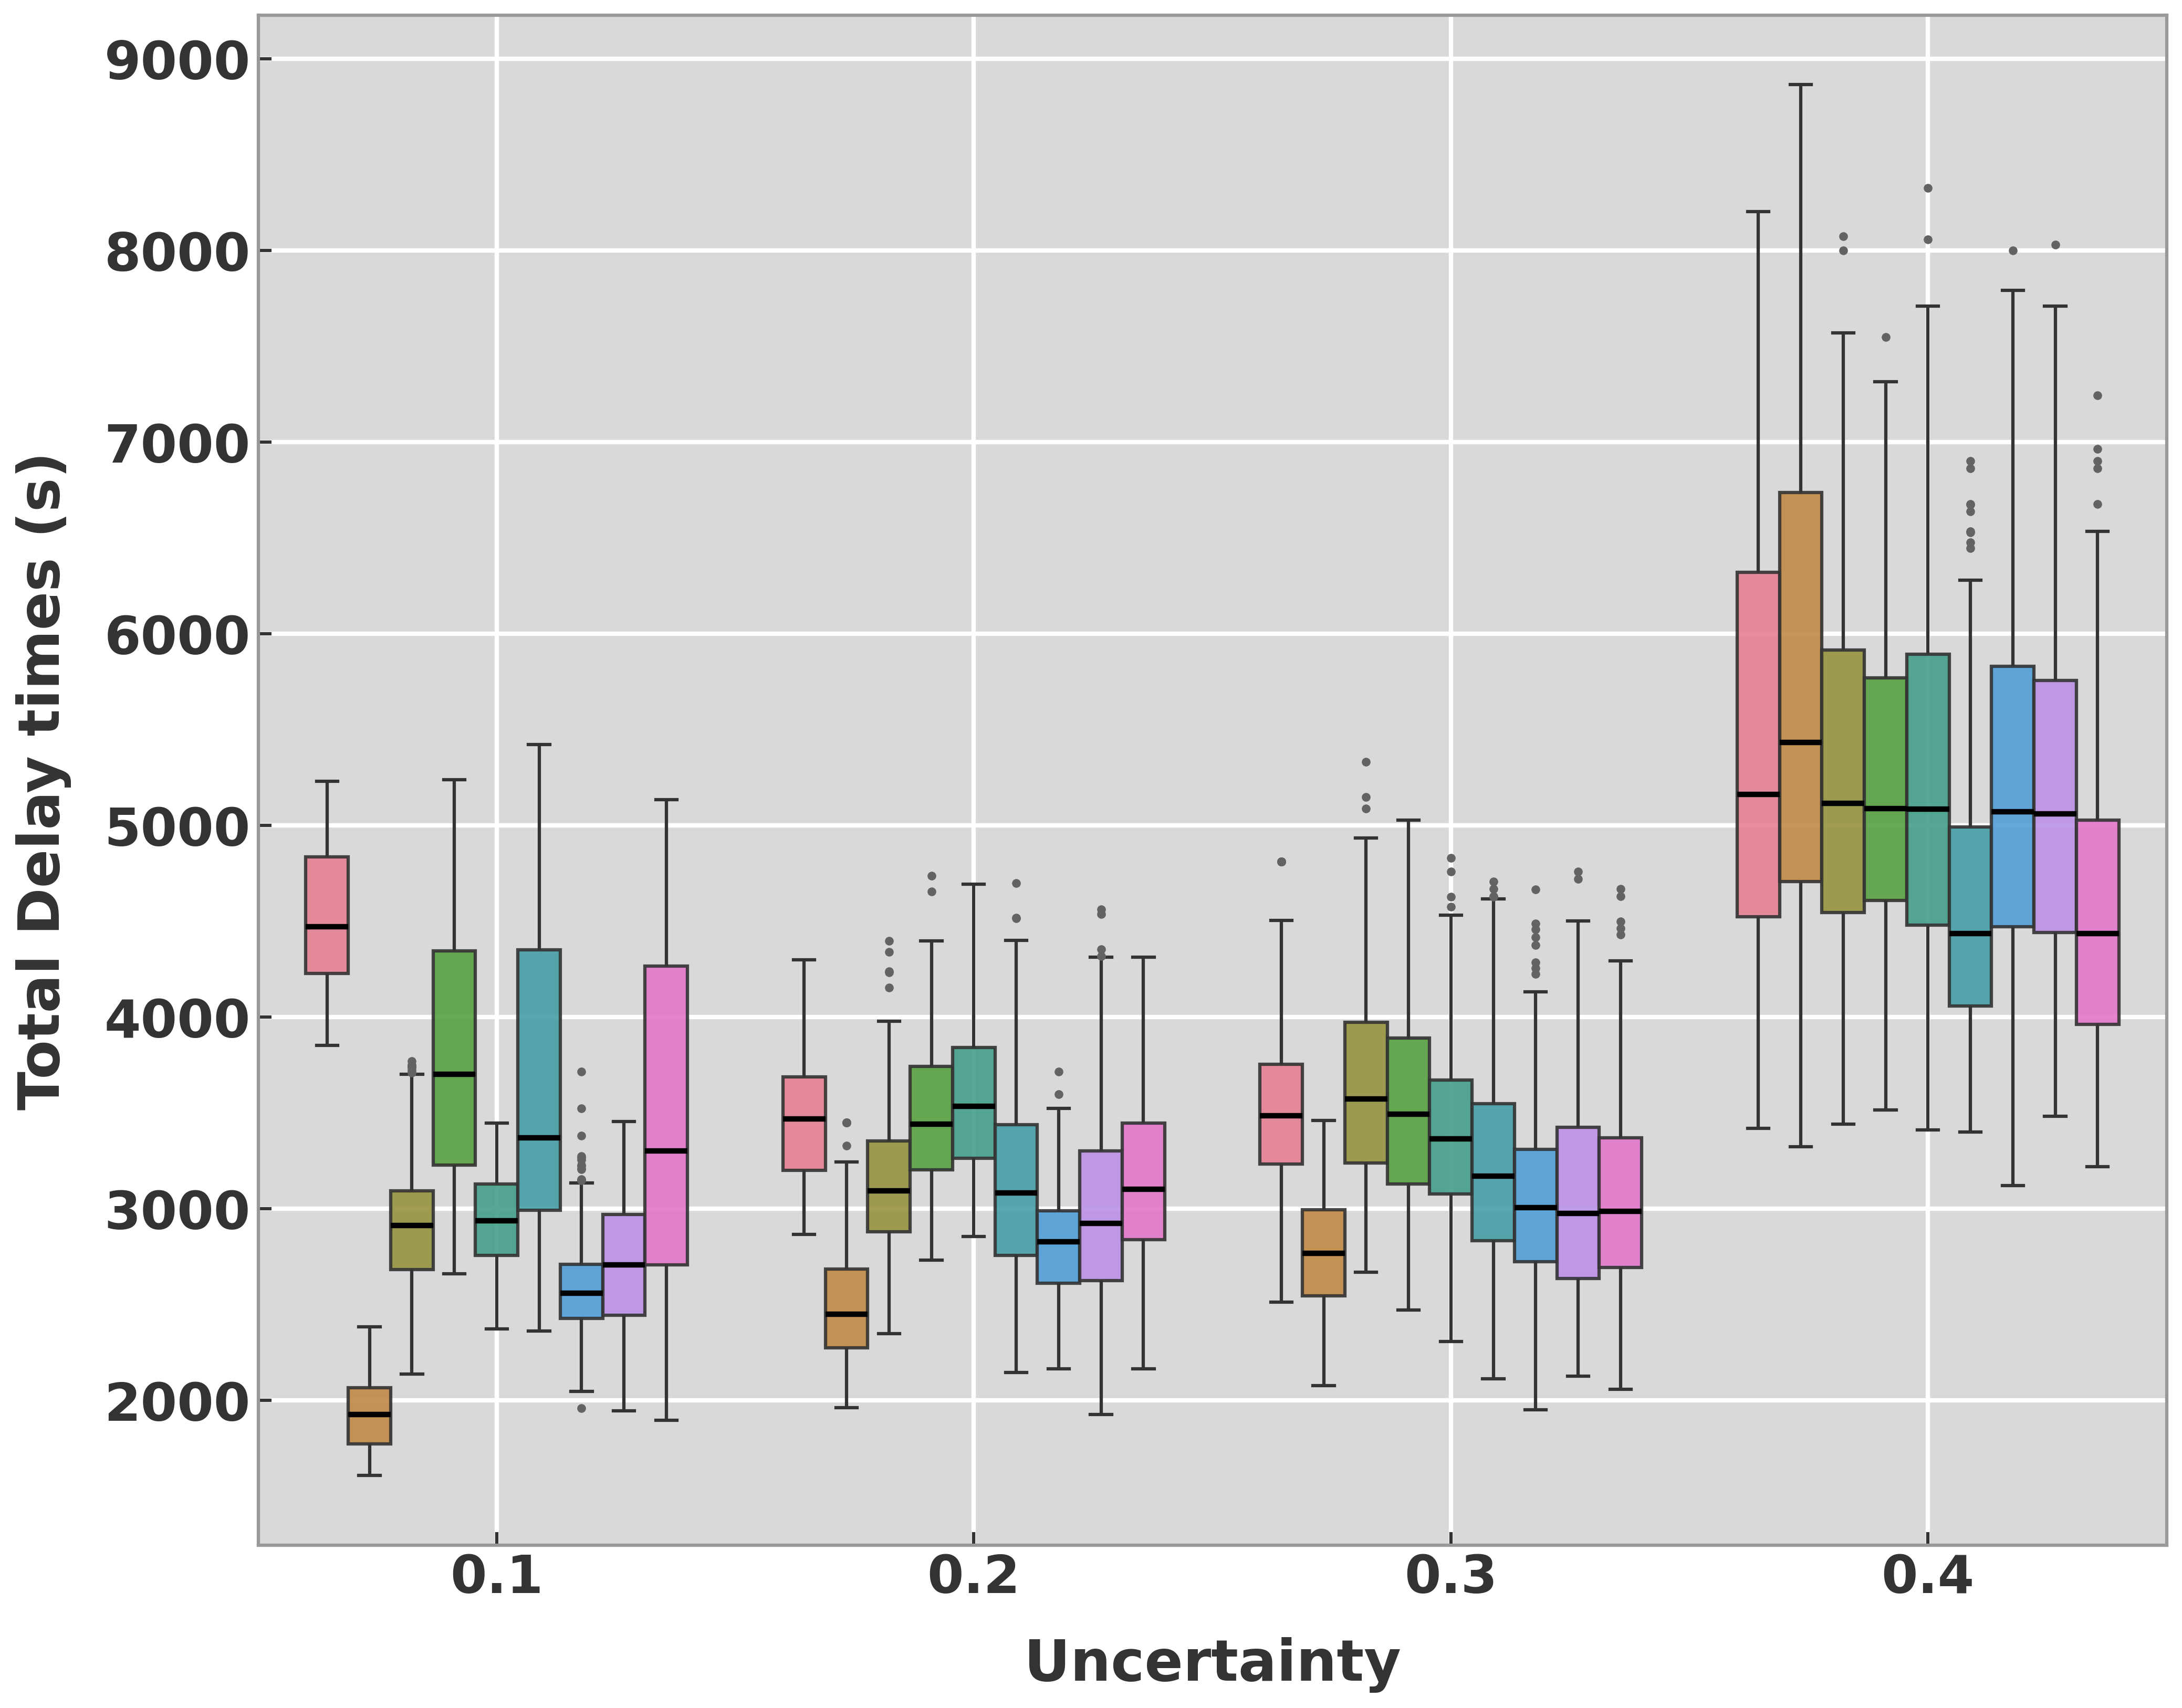
\includegraphics[width=0.45\textwidth]{figures/Traffic_1.0/traffic_1.0_total_delay.png}
    }
    \hfill
    \subfloat[Traffic density = 1.1\label{fig:delay_d}]{
        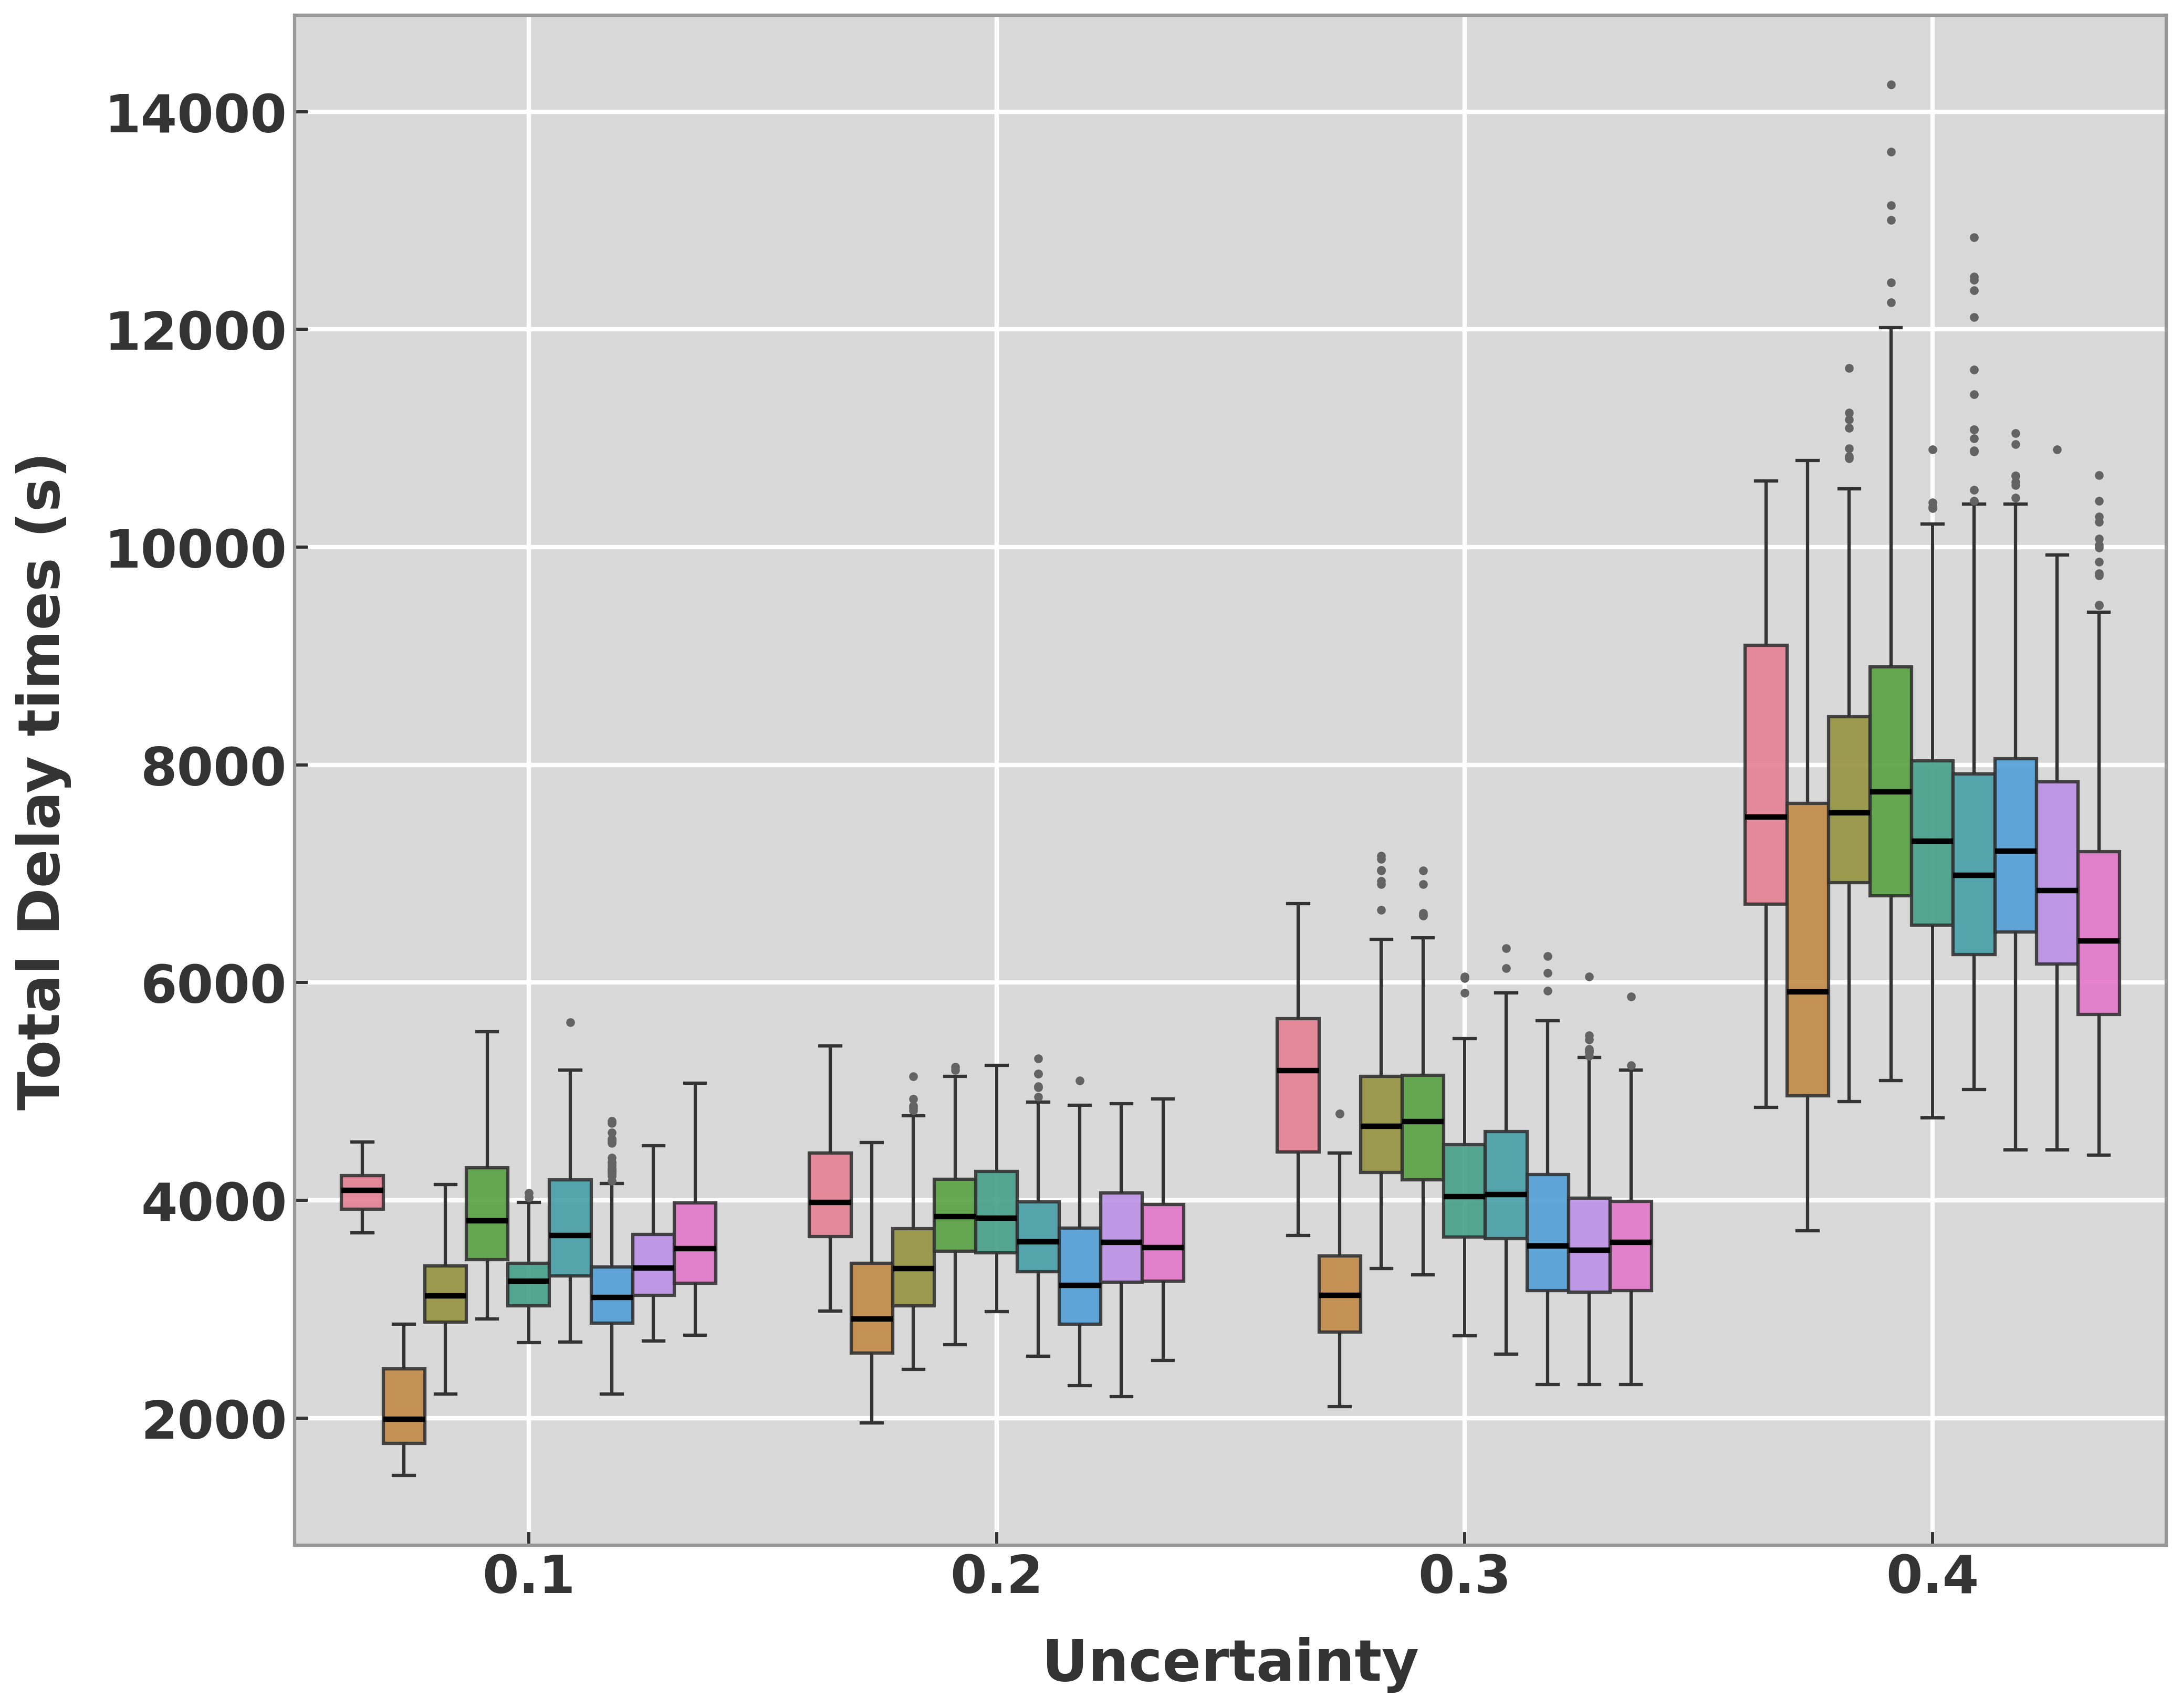
\includegraphics[width=0.45\textwidth]{figures/Traffic_1.1/traffic_1.1_total_delay.png}
    }
    
    % Row 3 (centered single image)
    \centering
    \subfloat[Traffic density = 1.2\label{fig:delay_e}]{
        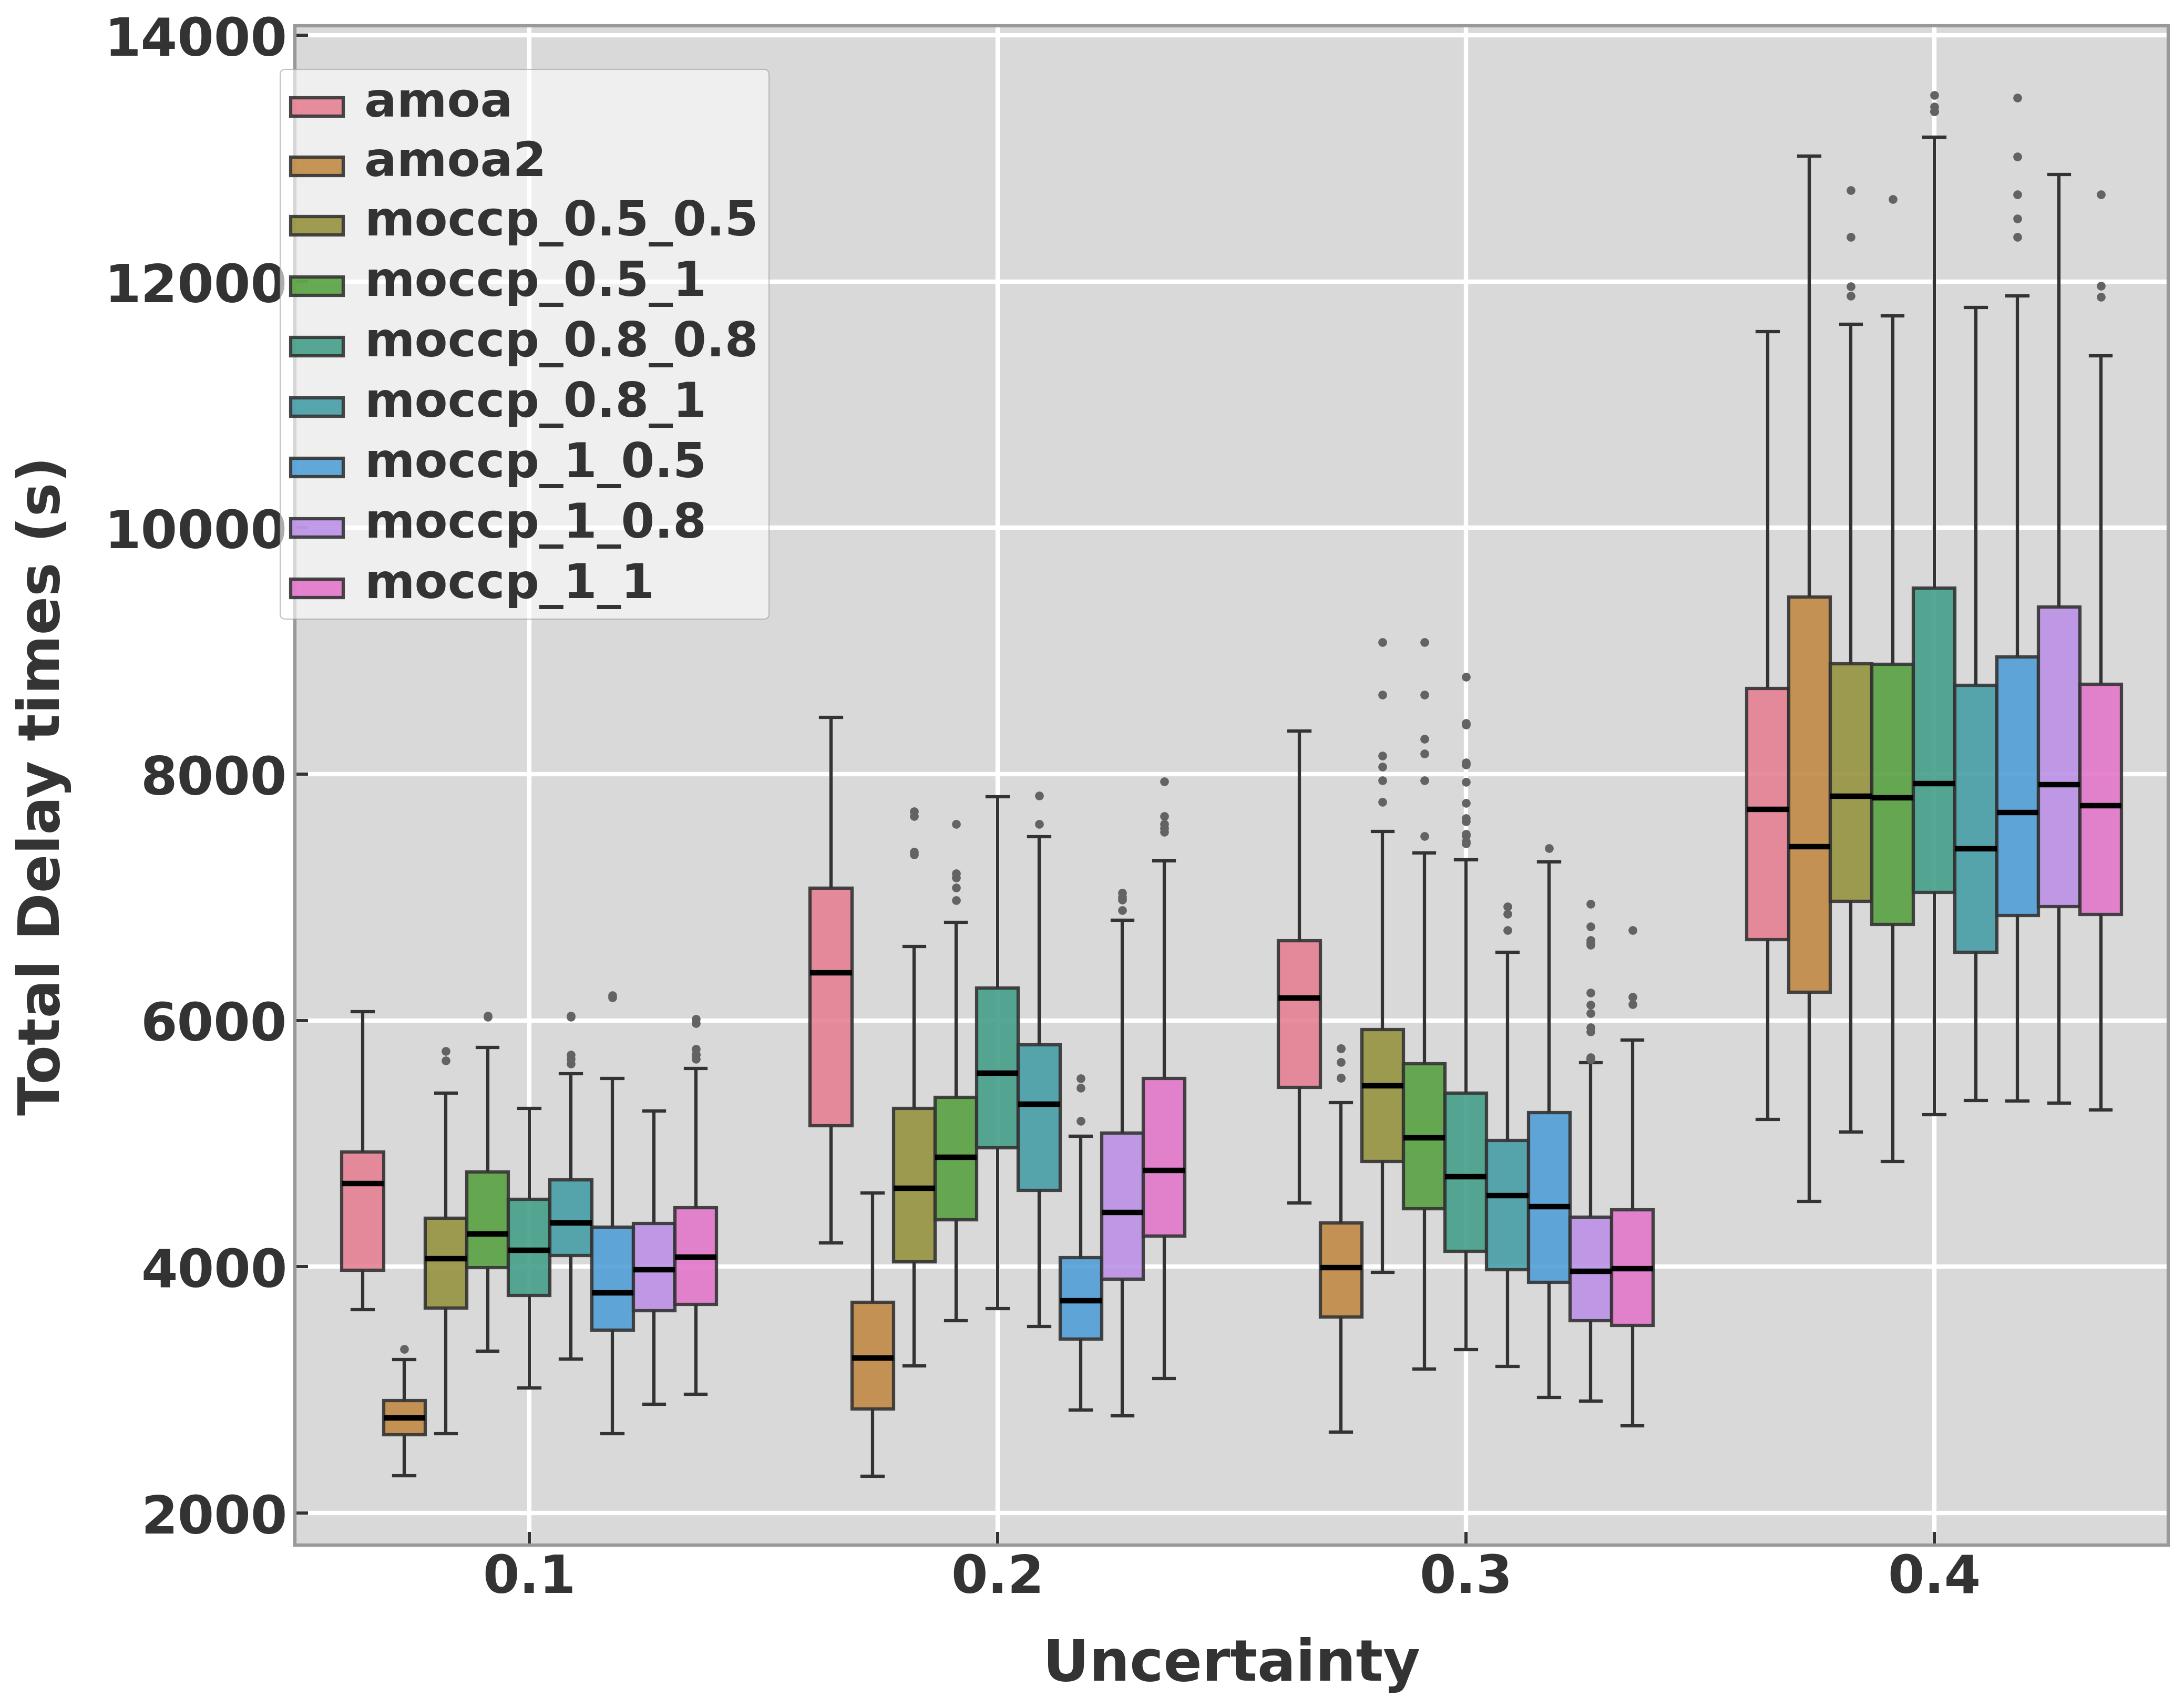
\includegraphics[width=0.45\textwidth]{figures/Traffic_1.2/traffic_1.2_total_delay.png}
    }
    
    \caption{Total delays under different traffic densities. In each sub figure, each group of nine bars has the same level of uncertainties.}
    \label{fig:delay}
\end{figure}

%======================================================
\begin{table*}[htp]
   \caption{Total taxiing distances (km) under different traffic densities (uncertainty level = 0.3). Each entry reports the total distance followed by the percentage difference from the corresponding minimum distance in parentheses. The minimum distances are obtained using Dijkstra's algorithm \cite{dijkstra2022note} and are 1043.7, 1090.8, 1214.4, 1354.4, and 1481.3 km for traffic densities 0.8, 0.9, 1.0, 1.1, and 1.2, respectively. Due to table width limitations, the CCP-AMOA* algorithms are denoted as $\alpha\_\beta$.}
    \label{Table:distance} 
    \scriptsize
    \begin{center}
        \resizebox{\textwidth}{!}{ % Resize the table to fit the text width
        \begin{tabularx}{\textwidth}{@{}>{\centering\arraybackslash}p{1cm}|*{8}{>{\centering\arraybackslash}p{1.45cm}}@{}}
            \toprule
            \textbf{Density} 
            & amoa & amoa2 & 0.5\_0.5 & 0.5\_1 & 1\_0.5 & 1\_1 & 0.8\_0.8 & 1\_0.8 \\
            \midrule
            0.8 
            & 1080.4 (3.5) & 1097.1 (5.1) & 1090.0 (4.4) & 1089.8 (4.4) 
            & 1103.9 (5.8) & 1102.6 (5.6) & 1091.6 (4.6) & 1102.7 (5.6) \\
            0.9 
            & 1130.7 (3.7) & 1153.4 (5.7) & 1140.2 (4.5) & 1140.5 (4.6) 
            & 1154.8 (5.9) & 1153.7 (5.8) & 1141.8 (4.7) & 1153.3 (5.7) \\
            1.0 
            & 1260.1 (3.8) & 1281.5 (5.5) & 1270.4 (4.6) & 1271.7 (4.7) 
            & 1286.0 (5.9) & 1285.8 (5.9) & 1273.1 (4.8) & 1285.2 (5.8)\\
            1.1 
            & 1411.1 (4.2) & 1436.1 (6.0) & 1418.2 (4.7) & 1418.5 (4.7) 
            & 1434.8 (5.9) & 1434.0 (5.8) & 1421.6 (5.0) & 1433.5 (5.8) \\
            1.2 
            & 1550.2 (4.7) & 1571.2 (6.1) & 1550.8 (4.7) & 1552.8 (4.8) 
            & 1568.9 (6.0) & 1569.2 (6.0) & 1553.9 (4.9) & 1567.5 (5.9) \\
            \midrule
            \textbf{Overall} 
            & 1260.1 (3.8) & 1281.5 (5.5) & 1270.4 (4.6) & 1271.7 (4.7) 
            & 1286.0 (5.9) & 1285.8 (5.9) & 1273.1 (4.8) & 1285.2 (5.8)\\
            \bottomrule
        \end{tabularx}
        }
    \end{center}
\end{table*}
%======================================================

\vspace{0.5em}
\textbf{Total taxiing distances comparison.}
\vspace{0.5em}

To further investigate and compare the routing algorithms, the total taxiing distances under different traffic densities are reported in Table~\ref{Table:distance}. Overall, the baseline algorithm \texttt{amoa} consistently yields the shortest taxiing distances, whereas \texttt{amoa2} produces significantly longer routes. This is expected, as \texttt{amoa2} adopts a more conservative strategy by considering worst-case estimates, which likely helps avoid conflicts and contributes to its relatively low total delays observed in simulations. For the CCP-AMOA* algorithms, the confidence level associated with the taxiing time objective appears to have a dominant influence on route length. For example, comparing \texttt{moccp\_0.5\_1} with \texttt{moccp\_1\_1}, or \texttt{moccp\_0.8\_0.8} with \texttt{moccp\_1\_0.8}, shows that a higher confidence level for taxiing time leads to longer distances, consistent with the observed reductions in delay. Furthermore, when confidence levels for both objectives increase (\texttt{moccp\_0.5\_0.5}, \texttt{moccp\_0.8\_0.8}, \texttt{moccp\_1\_1}), the allocated routes become progressively longer. Notably, some of the best-performing algorithms identified earlier, such as \texttt{moccp\_1\_0.5} and \texttt{moccp\_1\_0.8}, tend to allocate longer routes, while \texttt{moccp\_0.8\_0.8} achieves relatively shorter taxiing distances without sacrificing overall performance. An overall comparison of these top three algorithms is summarised in Table~\ref{Table:comparison}. \blue{These phenomena are partially consistent with previous studies that optimise taxiing time alone under uncertainty, where longer taxiing distances are often associated with lower total delay~\cite{wang2021chance}. In such cases, allocating longer routes typically corresponds to proactive detours that help avoid potential conflicts in advance, thereby reducing expected delays under uncertainty. However, a distinct difference arises when fuel consumption is introduced as a second optimisation objective. In the bi-objective setting considered in this work, longer taxiing routes may still involve detour-based strategies, achieving low total delay and low fuel consumption at the cost of moderate taxiing time. In contrast, shorter taxiing routes can also achieve competitive overall performance by prioritising reduced taxiing time, although this generally comes with higher fuel consumption (e.g., \texttt{moccp\_0.8\_0.8}). In these cases, a moderate increase in total delay or fuel consumption is acceptable because the expected taxiing time remains sufficiently low. This behaviour is not reported in prior studies that focus solely on taxiing time uncertainty~\cite{wang2021chance}, and it highlights how the inclusion of fuel consumption fundamentally alters the trade-off structure and routing strategies under uncertainty.}

%======================================================
\begin{table}[htp]
    \centering
    \caption{Qualitative comparison of three CCP-AMOA* algorithms across key performance metrics.}
    \label{Table:comparison}
    \normalsize
    \begin{tabular}{lcccc}
        \toprule
        \textbf{Algorithm} 
        & \textbf{Taxiing Time} 
        & \textbf{Fuel Consumption} 
        & \textbf{Total Delay} 
        & \textbf{Taxiing Distance} \\
        \midrule
        \texttt{moccp\_1\_0.5} 
        & Moderate 
        & Low 
        & Low 
        & Long \\
        
        \texttt{moccp\_1\_0.8} 
        & Moderate 
        & Low 
        & Moderate 
        & Long \\
        
        \texttt{moccp\_0.8\_0.8} 
        & Low 
        & Moderate 
        & High 
        & Short \\
        \bottomrule
    \end{tabular}
\end{table}
%======================================================

Typically, we illustrate the routes allocated to one departure aircraft under traffic density 1 and uncertainty level 0.3 with preference (0.5,0.5) by various algorithms: \texttt{moccp\_0.8\_0.8}, \texttt{moccp\_1\_0.5}, \texttt{moccp\_1\_0.8}, \texttt{amoa2}, and \texttt{amoa}. As shown in Fig.~\ref{Fig:route}, the routing decisions diverge notably as the aircraft approaches the runway exit for takeoff. Specifically, \texttt{amoa} allocates the shortest route, \texttt{moccp\_1\_0.5} and \texttt{moccp\_1\_0.8} allocate the longest routes, while \texttt{amoa2} and \texttt{moccp\_0.8\_0.8} allocate routes of intermediate length. Notably, this region represents a high-traffic hotspot where multiple aircraft converge for takeoff. In such scenarios, allocating slightly longer taxiing routes can offer greater temporal and spatial buffers, helping to absorb operational uncertainties, and potentially reduce fuel consumption through fewer stops. Although only the routes of one aircraft are visualised, it demonstrates how the proposed algorithms generate robust routes for AGM under uncertainties.

%======================================================
\begin{figure}[H]
	\centerline{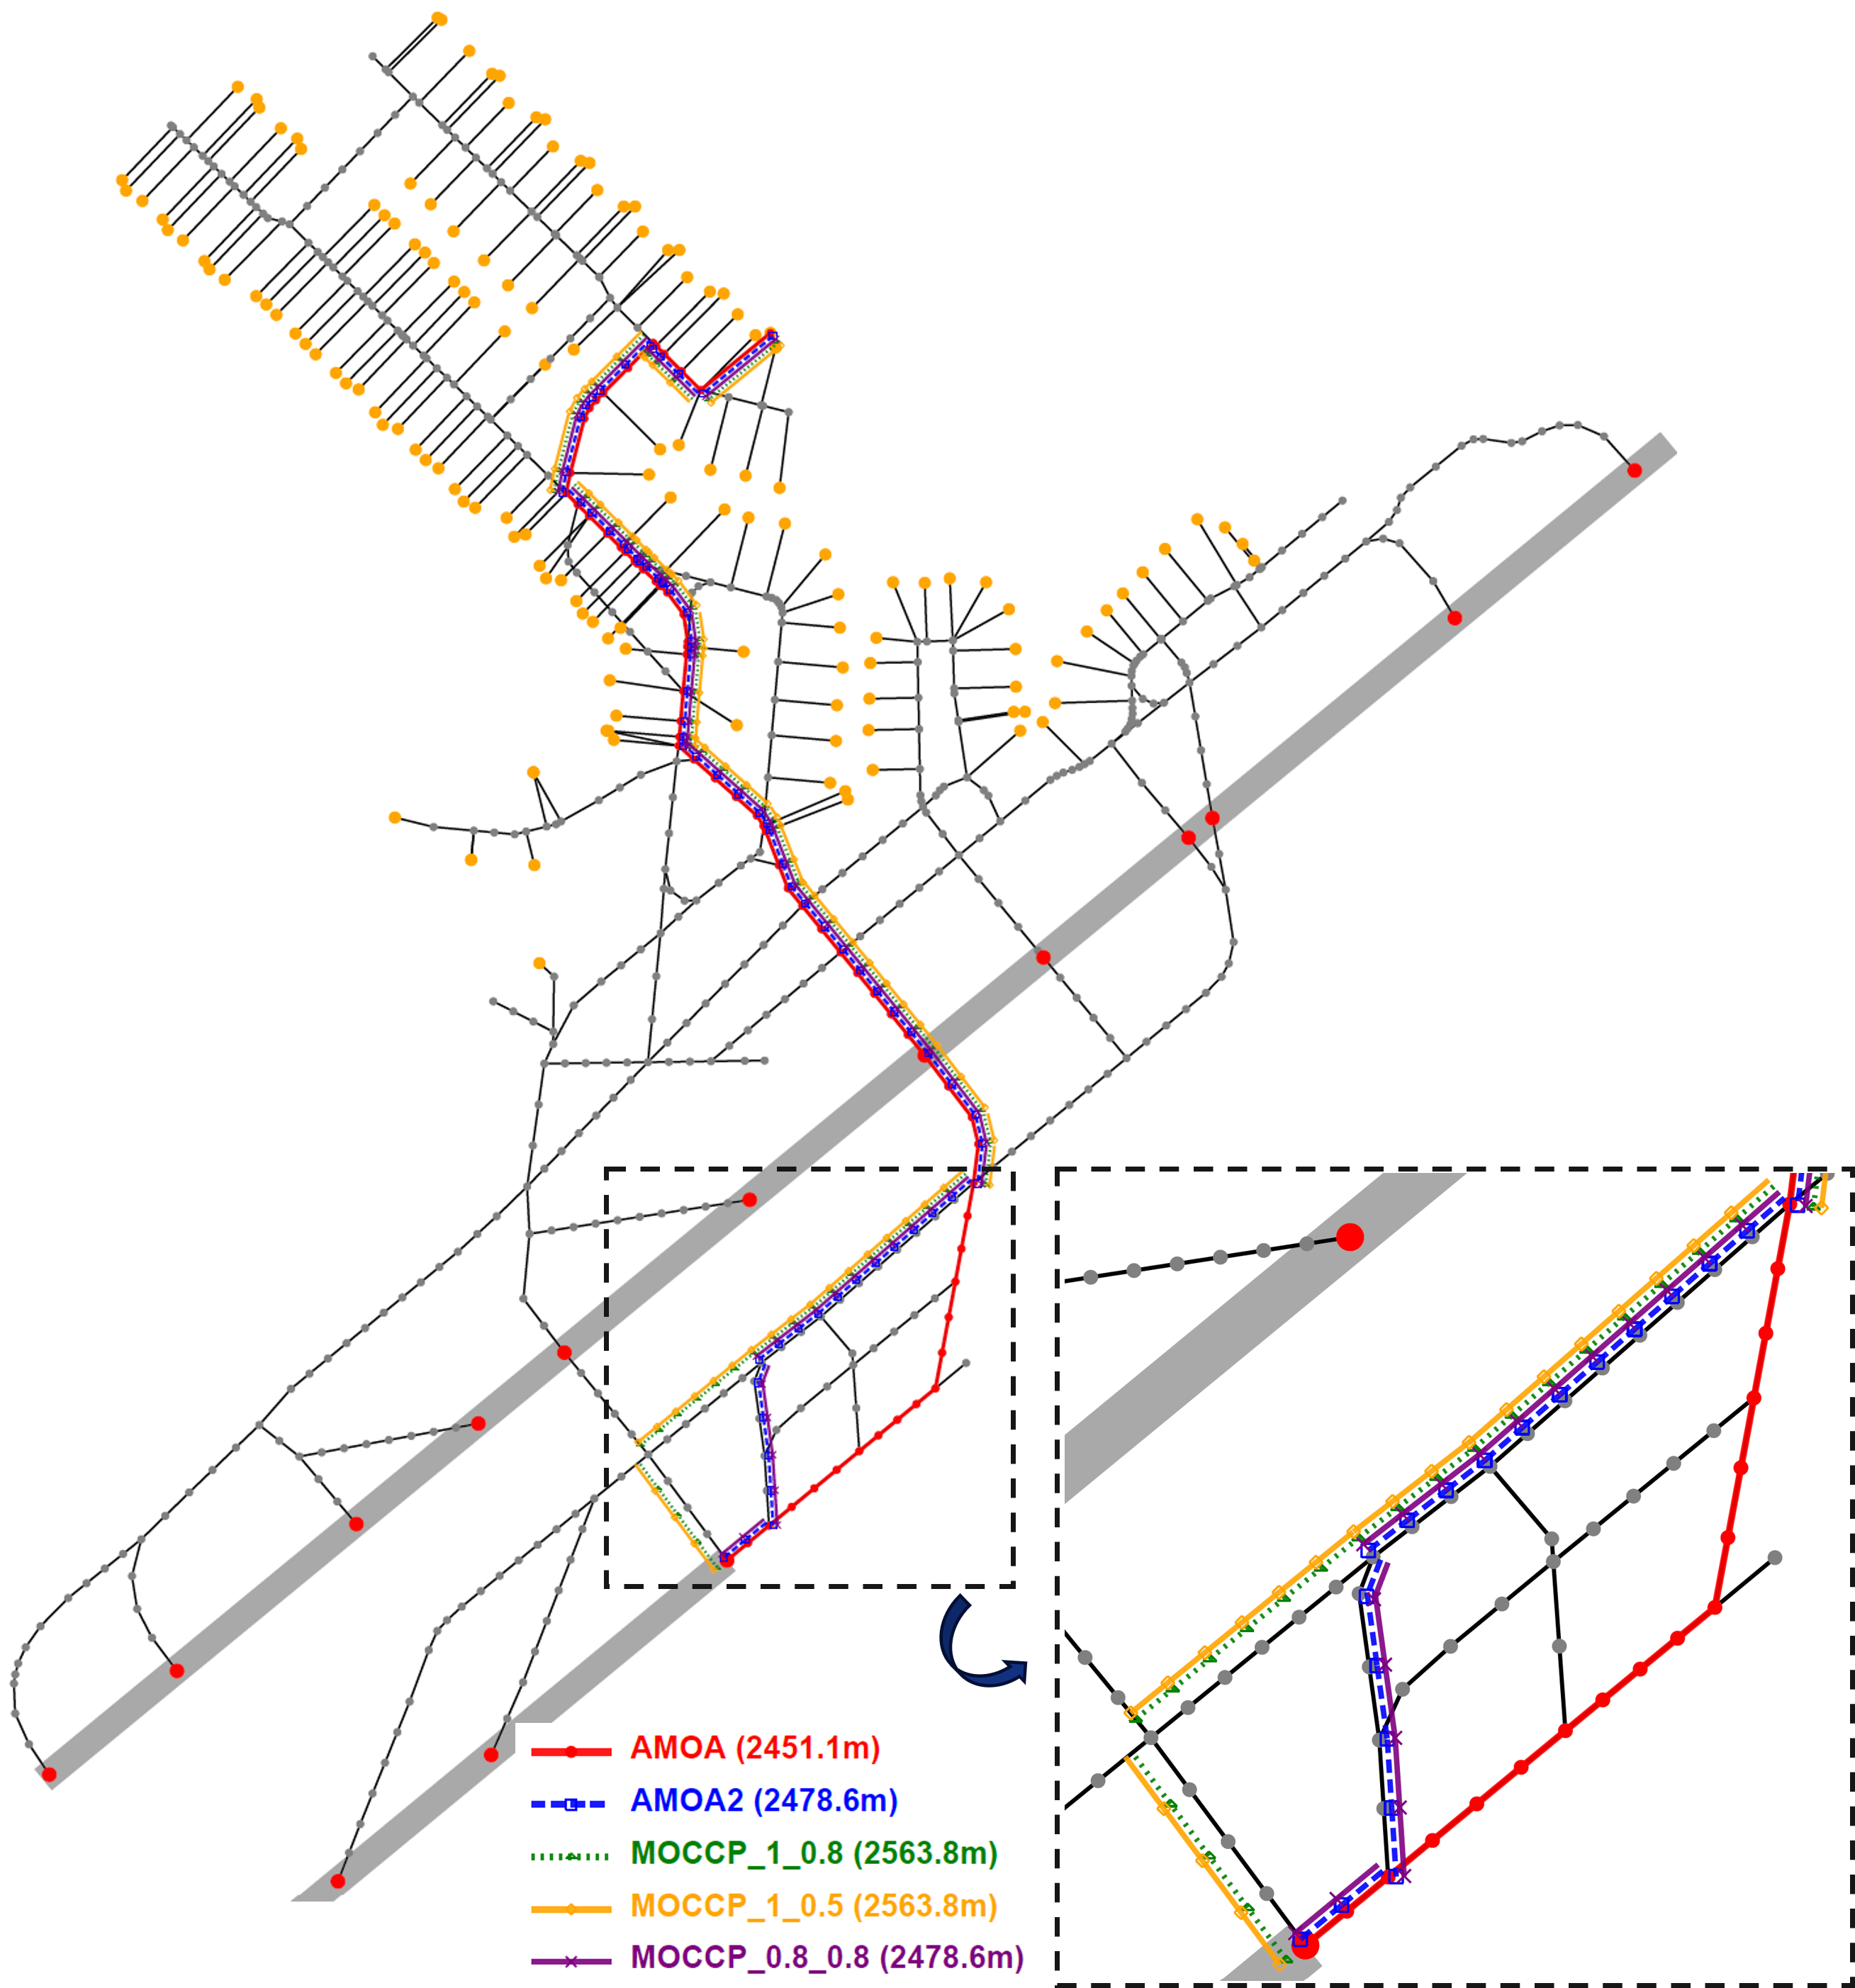
\includegraphics[width=4in]{figures/Route visualization/algorithms4.png}}
	\caption{Routes allocated by different algorithms under traffic density 1 and uncertainty level 0.3 with preference (0.5,0.5), with the relevant segments magnified for clarity. Each label indicates the algorithm used and the corresponding route length. In the magnified area, the blue and purple routes overlap, as do the yellow and green ones. \blue{Offsets between overlapping lines are added for better distinguish.}}
	\label{Fig:route}
	\vspace*{-0.5pc}
\end{figure}
%======================================================

\vspace{0.5em}
\textbf{Runtime comparison.}
\vspace{0.5em}



\begin{table}[htbp]
\centering
\caption{Average runtime (s) per algorithm across different traffic densities.}
\label{tab:avg_runtime_all}
\normalsize
\begin{tabular}{l r r r r r}
\toprule
\textbf{Algorithm} & \textbf{0.8} & \textbf{0.9} & \textbf{1.0} & \textbf{1.1} & \textbf{1.2} \\
\midrule
amoa             & \num{68} & \num{77} & \num{82} & \num{102} & \num{114} \\
amoa2            & \num{70} & \num{82} & \num{86} & \num{105} & \num{117} \\
moccp\_0.5\_0.5  & \num{1916} & \num{1978} & \num{2291} & \num{2693} & \num{3097}  \\
moccp\_0.5\_1  & \num{1902} & \num{1937} & \num{2305} & \num{2642} & \num{3071} \\
moccp\_0.8\_0.8  & \num{1875} & \num{1983} & \num{2375} & \num{2577} & \num{3093} \\
moccp\_0.8\_1    & \num{1859} & \num{1935} & \num{2370} & \num{2643} & \num{3026}  \\
moccp\_1\_0.5    & \num{1900} & \num{1977} & \num{2391} & \num{2658} & \num{3097} \\
moccp\_1\_0.8    & \num{1834} & \num{1974} & \num{2312} & \num{2668} & \num{3027} \\
moccp\_1\_1    & \num{1847} & \num{1977} & \num{2403} & \num{2630} & \num{3031} \\

% Add more algorithms here if needed
\bottomrule
\end{tabular}
\end{table}

Finally, we report the average runtime for each traffic density across all algorithms to assess their computational efficiency. As shown in Table~\ref{tab:avg_runtime_all}, the runtime for all algorithms increases with traffic density. Notably, the CCP-AMOA* algorithms require nearly 30 times more runtime than the baseline algorithms, which corresponds to the number of MC simulations performed.~\blue{Note that since all flight information is known in advance, the computation can be performed offline, making runtimes on the order of tens of minutes acceptable despite being higher than those of the baselines.} However, since candidate routes generation and time windows update in each simulation are independent tasks, these processes are inherently parallelisable. \blue{To further investigate the practical impact of this computational cost, we additionally implemented a parallelised version of the CCP-AMOA* algorithms and evaluated it under a traffic density of 1.0 using 8 CPU cores on the Apocrita high-performance computing cluster at Queen Mary University of London (\url{http://doi.org/10.5281/zenodo.438045}). In this setting, the average runtime of \texttt{moccp\_0.5\_0.5} at density 1.0 is reduced from 2291\,s to 1124\,s with parallel execution, while \texttt{moccp\_0.5\_1} decreases from 2305\,s to 1141\,s. Similar reductions are observed for the other CCP-AMOA* variants, with runtimes approximately halved (e.g., from 2375\,s to 1125\,s for \texttt{moccp\_0.8\_0.8} and from 2403\,s to 1199\,s for \texttt{moccp\_1\_1}). These results demonstrate that the algorithm benefits effectively from parallel execution and that the practical impact of its computational complexity can be substantially mitigated when moderate multi-core resources are available.}
\section{Conclusion}

In this paper, a multi-objective chance-constrained programming model is proposed for Airport Ground Movement optimisation to address uncertainties in aircraft taxiing time and fuel consumption. Since it is non-trivial to derive analytical expressions under uncertainties, a Monte Carlo simulation approach based on the Follow the Greens guidance system is adopted to model the uncertainties. Building upon the MOCCP model, a CCP-AMOA* algorithm is developed to sequentially allocate robust routes for aircraft. Using benchmark scenarios from Manchester Airport, the MC simulations reveal that the impact of uncertainties on taxiing time and fuel consumption varies considerably across the airport’s taxiway network. Subsequent extensive route allocation simulations compare the proposed CCP-AMOA* algorithms with deterministic baselines. Results demonstrate that \texttt{moccp\_1\_0.5}, \texttt{moccp\_1\_0.8}, and \texttt{moccp\_0.8\_0.8} outperform others in terms of generating flimsily robust efficient points, reducing economic cost, and minimising total delay. Further analysis on each objective (e.g., taxiing time, fuel consumption, separately) and taxiing distance reveals how varying confidence levels affect the trade-off between taxiing time and fuel consumption. For instance, \texttt{moccp\_1\_0.5} and \texttt{moccp\_1\_0.8} tend to allocate longer taxi routes that result in lower fuel consumption with moderate taxiing time, while \texttt{moccp\_0.8\_0.8} allocates routes of moderate length, yielding balanced performance in both objectives. \textcolor{blue}{It should be noted that the specific parameter values (e.g., (1, 0.5), (0.8, 0.8)) are case-specific examples derived from MAN and serve to demonstrate the behavioural tendencies of the method. They should not be interpreted as prescriptive optimal configurations for other airports.} Besides, longer routes provide greater temporal and spatial buffers, helping to absorb uncertainties, leading to fewer delays. Although the runtime of the proposed algorithms is significantly longer than that of the baselines, approximately 30 times due to the number of simulation runs, which can be mitigated with parallel computing. Under ideal computational conditions, runtimes could be brought closer to those of baselines. \textcolor{blue}{When applying the proposed framework to other airports, appropriate parameter tuning based on the specific operational context and objectives would be required. The key generalisable insight lies in the consistent trade-off trends between objectives across varying conditions. Furthermore, the study reveals how different confidence-level combinations shape the algorithm's behaviour within the proposed framework.}

For future work, several directions can be explored. \blue{First, the preliminary experiments suggest that parallel computing is a promising avenue for reducing the computational runtime of the proposed algorithm. A more systematic exploration of parallel implementations and scalability under different resource configurations is worth exploring.} Second, as discussed in the introduction, AGM is interconnected with other airport operations, such as runway scheduling \cite{ikli_aircraft_2021}, and uncertainties from these interdependent processes can propagate to taxiing operations. Although integrated approaches to airport ground operations have been proposed \cite{weiszer2015integrated}, how uncertainties propagate within such systems and how they can be mitigated remain largely unexplored. \blue{Third, the FtG model's pilot driving component can be readily replaced with more realistic formulations leveraging richer empirical or context-specific parameter distributions as comprehensive datasets become available, thus enhancing the model’s generality and applicability. Similarly, the fuel consumption model can be substituted with more advanced alternatives (e.g., machine learning–based models) once additional empirical data become available. Furthermore, benchmark fuel consumption data would enable data-driven methods to learn uncertainty distributions directly from historical data, similar to taxiing time prediction \cite{wang2021aircraft}, further improving decision-making realism and accuracy. Finally, global optimisation, such as multi-objective evolutionary algorithms, offers a promising approach for addressing the AGM problem under uncertainties. However, the algorithm complexity and how to evaluate objective values with low computational overhead should be investigated before implementation.}
\section{Acknowledgements}
The authors acknowledge the financial support provided by the joint scholarship program of the China Scholarship Council and Queen Mary University of London (Grant No. 202306370044).
\bibliographystyle{IEEEtran}
\clearpage
\bibliography{references}

\end{document}
